\documentclass[12pt,a4paper, usenames, dvipsnames]{article}
\usepackage{graphicx}
\usepackage{xcolor}


\usepackage[ngerman]{babel}
\usepackage[utf8]{inputenc}
\usepackage{mathtools}
\usepackage{amsmath}
\allowdisplaybreaks
\usepackage{amssymb}
\usepackage{geometry}
\usepackage{tikz}
\usepackage{float}
\usepackage{verbatim}

\usepackage{autobreak}

%\usepackage{algorithm} 
%\usepackage{algpseudocode} 
\usepackage[german, ruled, vlined]{algorithm2e}

\usepackage{amsthm}


\newtheoremstyle{mystyle}% name
{15pt}% Space above
{5pt}% Space below
{\itshape}% Body font
{}% Indent amount: 
{\bf}% Theorem head font
{}% Punctuation after theorem head
{\newline}% Space after theorem head
{}% Theorem head 

\theoremstyle{mystyle}
\newtheorem{definition}{Definition}


\newtheoremstyle{definition}% name
{15pt}% Space above
{5pt}% Space below 
{}% Body font
{}% Indent amount: Indent amount: empty = no indent, \parindent = normal paragraph indent
{\bf}% Theorem head font
{}% Punctuation after theorem head
{\newline }% Space after theorem head: Space after theorem head: { } = normal interword space; \newline = linebreak
{}% Theorem head spec (can be left empty, meaning `normal')

\theoremstyle{definition}

\newtheorem{bsp}{Beispiel}[definition]

\usepackage[nottoc]{tocbibind}

\usepackage[onehalfspacing]{setspace}

\usepackage{stmaryrd}

\usepackage{microtype}

\usepackage{booktabs}

\usepackage{array}

\usepackage{hyperref}
\hypersetup{
    colorlinks=true,
    linkcolor=black,
    filecolor=black,      
    urlcolor=blue,
    citecolor=black
}

\usepackage{subfigure}

\usepackage[compact]{titlesec}     


\usepackage[center]{caption}


\pagestyle{plain}

\usepackage[backend=biber]{biblatex}

\addbibresource{references.bib}

\usepackage{adjustbox}

\newcommand{\Gtwo}{\ensuremath{G_{2\times 2\times 2}}}

\newcommand{\Gthree}{\ensuremath{G_{3\times 3\times 3}}}

\newcommand{\Ttwo}{2$\times$2$\times$2-}

\newcommand{\Tthree}{3$\times$3$\times$3-}

\clubpenalty = 10000
\widowpenalty = 10000
\displaywidowpenalty = 10000


\geometry{
  paper=a4paper, % Change to letterpaper for US letter
  top=3cm, % Top margin
  left=2cm, % Left margin
  right=3cm, % Right margin
  %showframe, % Uncomment to show how the type block is set on the page
}

\setlength{\parindent}{0em}

\setlength{\parskip}{1.3ex}

\pagenumbering {arabic} 

\titlespacing*{\section}{0pt}{10ex plus 1ex minus .2ex}{4.3ex plus .2ex}









\begin{document}

\pagenumbering{roman}


\begin{titlepage}
	\centering
	{\scshape\LARGE Technische Universität Dortmund \par}
	Fakultät für Informatik \par
	Lehrstuhl 14 für Software Engineering \par
	\vspace{1cm}
	{\scshape\Large Bachelorarbeit \par }
	\vspace{1.5cm}
	{\huge\bfseries  Gruppentheorie des \\ 2$\times$2$\times$2 Zauberwürfels und dessen Lösungsalgorithmen \par}
	\vspace{2cm}
	{\Large\itshape Pina Kolling\par}
	\vspace{0.5cm}
	{Abgabe: Mai 2021 \par }
	\vfill
	betreut von\par
	Dr. \L ukasz \textsc{Czajka} \par 
	und \par 
	M. Sc. Christoph \textsc{Stahl} 

	\vfill

% Bottom of the page
	{\large \today\par}
\end{titlepage}

\setcounter{page}{1}

%\setstretch{0.6}

\newgeometry{
  top=2.5cm, % Top margin
    left=2cm, % Left margin
  right=3cm % Right margin
}

\begin{spacing}{0.45}



\tableofcontents

\end{spacing}

\newgeometry{
  top=3cm, % Top margin
  left=2cm, % Left margin
  right=3cm % Right margin
}


%\setstretch{1.5}





\newpage

\pagenumbering{arabic}

\setcounter{page}{1} 
%

%
%
%
%
%=======================================================================================================
%
%
%
%
%
\section{Einleitung}

\label{Kapitel_Einleitung}

Der \Tthree Zauberwürfel ist ein mathematisches Drehpuzzle, das 1974 von dem ungarischen Professor Ern\H{o} Rubik erfunden wurde. Er wollte damit seinen Studierenden helfen, dreidimensionale Probleme zu verstehen. Ern\H{o} Rubik selbst brauchte über einen Monat, um den \Tthree Würfel zum ersten Mal zu lösen.
Der sogenannte \textit{Rubik's Cube} wurde ab 1980 weltweit verkauft. Die Begeisterung für den Würfel war so groß, dass bereits 1982 die erste Weltmeisterschaft in Budapest stattfand. Der Gewinner war Minh Thai aus den USA, der den Würfel in $22,95$ Sekunden löste. \cite{RC} Die Zeiten zum Lösen des \Tthree Würfels wurden immer wieder unterboten.
Im Jahr 2018 löste der Chinese Yusheng Du den Würfel bei einem Wettbewerb in $3,47$ Sekunden und stellte damit einen neuen Weltrekord auf, der bis heute nicht gebrochen wurde \cite{rekord}.
Das Patent für den kleineren \Ttwo Würfel hat \textit{Rubik} im Jahr 1981 angemeldet \cite{patent}. Dieser Würfel ist Gegenstand dieser Arbeit.

Bis heute sind Kinder und Erwachsene gleichermaßen von den Zauberwürfeln begeistert.
Doch die Zauberwürfel sind nicht nur interessante Puzzle zur manuellen Lösung -- sie bieten beispielsweise auch die Möglichkeit, sie maschinell mit Bild- und Farberkennung zu lösen. Außerdem können die Würfel als algebraische Strukturen dargestellt werden.

%
%
%
%
%=======================================================================================================
%
%
%
%
\subsection{Motivation} 




Der \Tthree Würfel ist Gegenstand zahlreicher Arbeiten \cite{JC, TD, DJ, TR, RMG, DDJT} und
%Die \textit{God's Number} -- das ist die maximal erforderliche Anzahl der nötigen Drehungen des optimalen Lösungswegs -- ist Gegenstand vieler Arbeiten und wurde oft berechnet und durch neue Algorithmen verbessert. 
%Die Berechnung der \textit{God's Number} des \Tthree Würfels ist wesentlich anspruchsvoller und dadurch auch interessanter als die des \Ttwo Würfels. 
wurde zudem schon mehrfach als Gruppe dargestellt und untersucht \cite{JC, TD, DJ}. Ziel dieser Arbeit ist es, das Wissen des \Tthree Würfels auf den \Ttwo Würfel zu übertragen. Der \Ttwo Würfel hat im Gegensatz zum \Tthree Würfel weniger Steine und keine Kantsteine -- dadurch ist der kleinere Würfel weniger komplex. Dafür kann der \Ttwo Würfel aber aufgrund der fehlenden Mittelsteine rotiert werden und so kann die Oberseite beliebig geändert werden. In dieser Arbeit wird das Wissen der Gruppe des \Tthree Würfels übertragen und angepasst und somit der \Ttwo Würfel mithilfe der Gruppentheorie dargestellt. Anhand dieser Gruppe können dann Erkenntnisse über den Würfel gewonnen werden. Dazu zählen unter anderem die Berechnung der Anzahl der möglichen Würfelkonfigurationen und die Erstellung eines Konzeptes zum Finden des optimalen Lösungswegs.

Wer die Lösungsalgorithmen des \Ttwo Zauberwürfels selber herleiten möchte, sollte dies vor dem Lesen dieser Arbeit tun, da diese hier teilweise erklärt und genutzt werden.

%
%
%
%
%=======================================================================================================
%
%
%
%
\subsection{Struktur} 

Diese Arbeit setzt sich aus 10 Kapiteln zusammen. Im Folgenden werden die Inhalte und Themen dieser Kapitel aufgelistet.

\begin{itemize}
\item[\textbf{\ref{Kapitel_Einleitung}}] In der Einleitung wird eine kurze Übersicht der Geschichte des Würfels gegeben. Außerdem befinden sich hier die Motivation und die Struktur.

\item[\textbf{\ref{Kapitel_Würfel}}] In diesem Kapitel wird der Aufbau des \Ttwo Würfels und die dazugehörige Terminologie erklärt. Außerdem werden die Grundzüge des Würfels definiert.

\item[\textbf{\ref{Kapitel_MathematischeGrundlagen}}] Hier werden die mathematischen Grundlagen erklärt. Dafür werden unter anderem Gruppen und andere algebraische Strukturen definiert und anhand von Beispielen erklärt.

\item[\textbf{\ref{Kapitel_KonfigurationDesWürfels}}] In dem Kapitel \textit{Konfiguration des Würfels} werden die Positionen der Steine und die Ausrichtung der Steine im Würfel erklärt und auf das mathematische Modell übertragen. Dabei wird die Konfiguration definiert. 

\item[\textbf{\ref{Kapitel_WürfelAlsGruppe}}] In diesem Kapitel wird die Gruppe des \Ttwo Würfels beschrieben und die Gleichheit von Zügen definiert. Außerdem werden Äquivalenzrelationen eingeführt, um die Rotationen des Würfels zu realisieren und es wird die Ordnung von Zügen definiert.

\item[\textbf{\ref{Kapitel_Untergruppen}}] Das Kapitel \textit{Untergruppen} befasst sich mit Beispieluntergruppen, Erzeugern und Cayleygraphen der Gruppe des \Ttwo Würfels.

\item[\textbf{\ref{Kapitel_ValideKonfigurationen}}] Hier wird die Anzahl der möglichen Würfelkonfigurationen und die Mächtigkeit der Trägermenge der Gruppe des \Ttwo Würfels berechnet und verglichen.

\item[\textbf{\ref{Kapitel_Lösung}}] In diesem Kapitel werden verschiedene Lösungsansätze und Algorithmen erklärt. Die Lösung des Wüfels durch einen Menschen wird anhand eines Beispiels schrittweise erklärt und es findet sich eine allgemeine Anleitung, mit der der \Ttwo Würfel immer gelöst werden kann.

\item[\textbf{\ref{Kapitel_MinUntergruppe}}] Hier wird die Untergruppe mit minimalen Grundzügen beschrieben, die den Würfel vollständig abbildet. Außerdem wird ein Konzept eingeführt, um den optimalen Lösungsweg des Würfels zu berechnen.  

\item[\textbf{\ref{Kapitel_Fazit}}] Am Schluss der Arbeit befindet sich die Zusammenfassung, das Ergebnis und der Ausblick.

\end{itemize}


%
%
%
%
%
%
%=======================================================================================================
%
%
%
%
%
%
\newpage
\section{Der \Ttwo Würfel}

\label{Kapitel_Würfel}

In diesem Kapitel werden die Grundlagen des \Ttwo \textit{Cubes} erklärt. Zuerst wird der Aufbau und die Terminologie des Würfels erläutert. Anschließend wird kurz auf die Unterschiede zwischen dem \Ttwo und dem \Tthree Würfel eingegangen. 
Außerdem werden die sechs Grundzüge des Würfels definiert und erklärt. Darauf basieren alle späteren Algorithmen und die Definition der Gruppe des Würfels.


%
%
%
%
%
%
%=======================================================================================================
%
%
%
%
\subsection{Terminologie}

Die Terminologie und der Aufbau des Würfels sind Grundlagen für die weiteren Kapitel.
Im Folgenden wird die Terminologie und der Aufbau des Würfels erklärt.



\begin{description}


\item[\Ttwo Würfel] (auch Zauberwürfel oder \textit{Cube}) 

Der Würfel setzt sich aus acht kleineren Würfeln zusammen.
In Abbildung \ref{Abbildung_WürfelUngelöstGelöst} ist er links verdreht und rechts im gelösten Zustand zu sehen. Der gelöste Zustand wird als Startkonfiguration bezeichnet.
Bei der Startkonfiguration (auch Grundposition, Grundstellung) des \Ttwo Würfels hat jede Seite 4 Farbflächen derselben Farbe. 
Bei dem verdrehten Würfel können sich die Steine des Würfels an anderen Positionen befinden und anders ausgerichtet sein.
\begin{figure}[h]
\centering
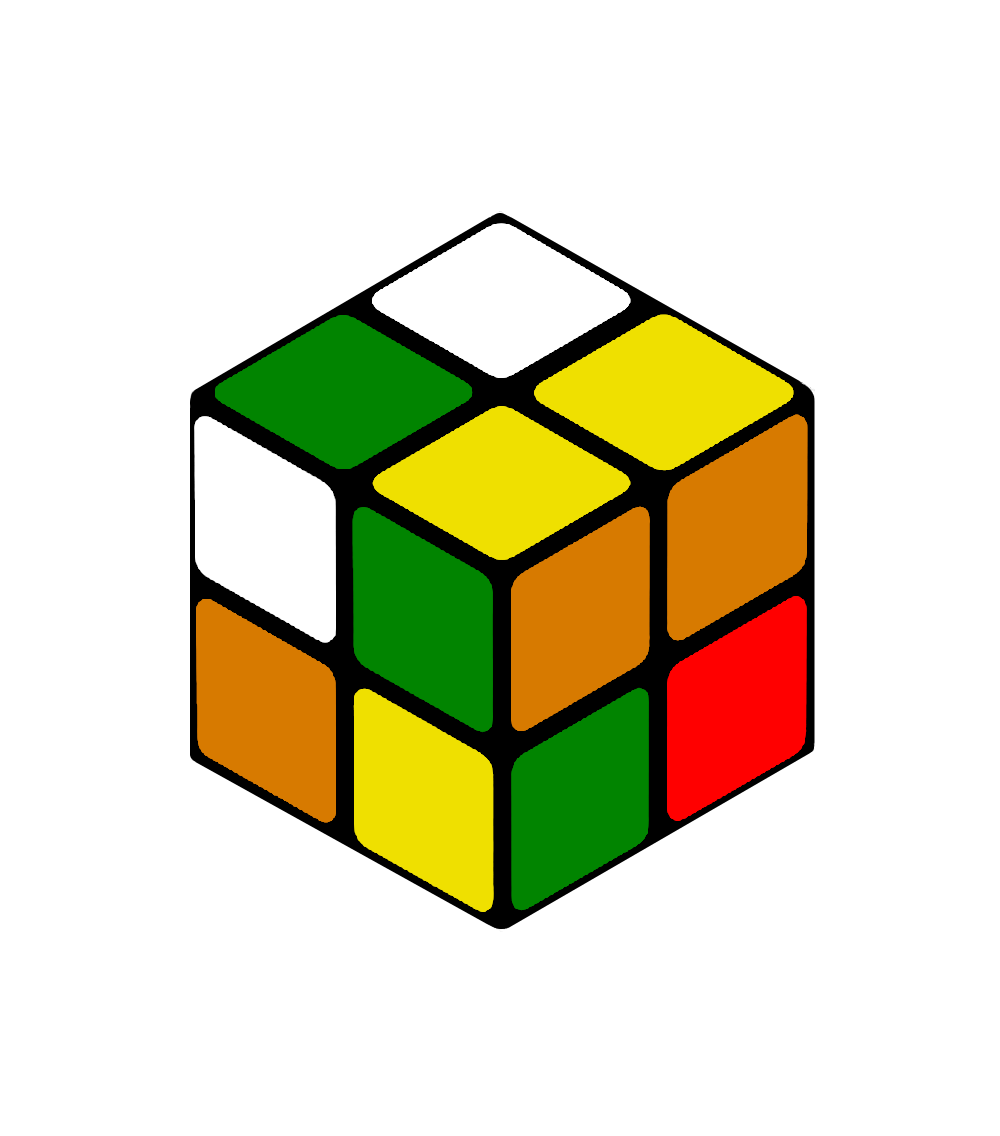
\includegraphics[scale=0.1]{2x2scrambled.png}
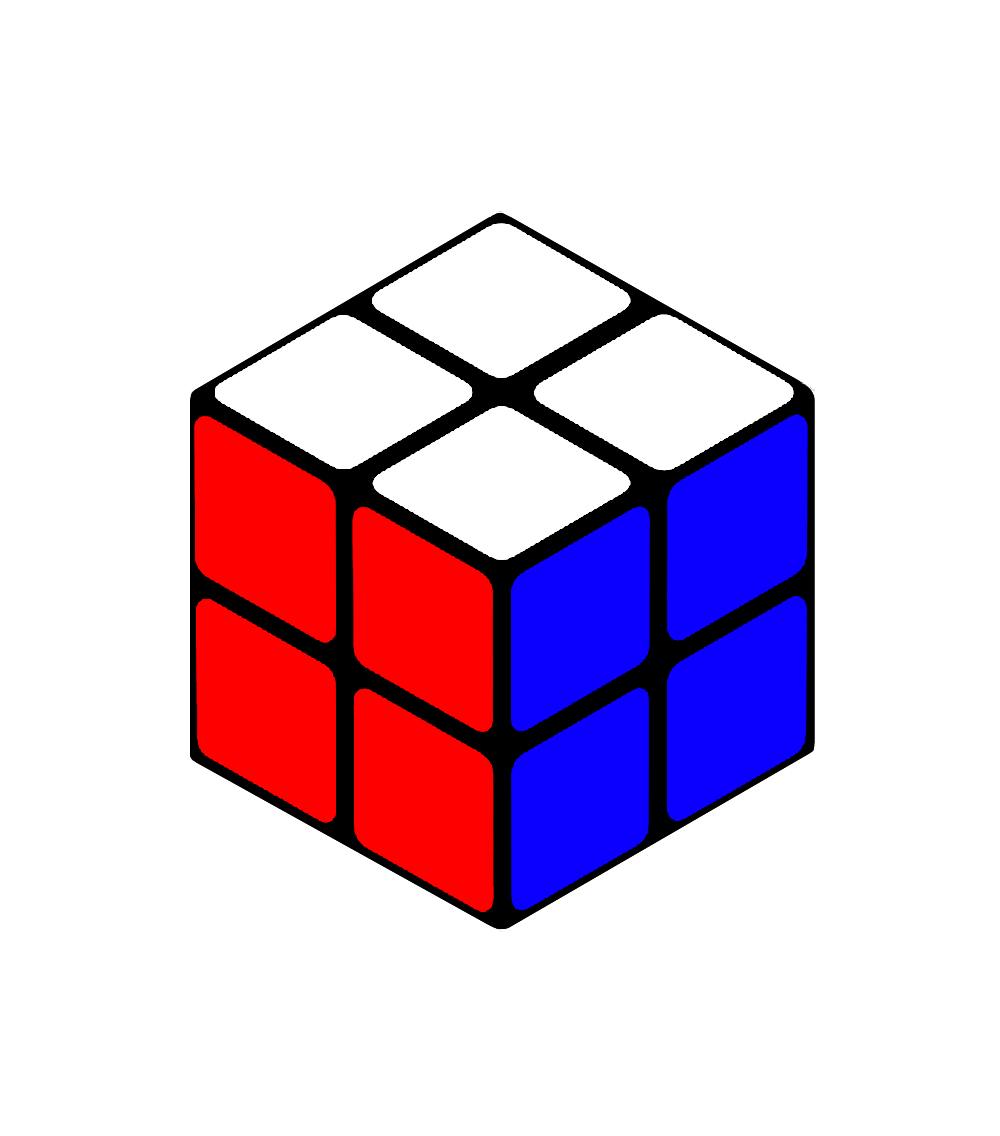
\includegraphics[scale=0.1]{2x2solved.png}
\caption[Ungelöster und gelöster \Ttwo Würfel]{Ungelöster und gelöster \Ttwo Würfel}
\label{Abbildung_WürfelUngelöstGelöst}
\end{figure}


\item[Eckstein und Farbfläche] \ \\
Ein \Ttwo Würfel besteht aus acht Ecksteinen (links in Abbildung \ref{Abbildung_Eckstein}), die jeweils drei Farbflächen (rechts in Abbildung \ref{Abbildung_Eckstein}) haben. Ein \Ttwo Zauberwürfel weist somit 24 Farbflächen auf. Die verschiedenen Farbpaare, die sich im gelösten Zustand jeweils gegenüberliegen, sind weiß und gelb; rot und orange; grün und blau.
\begin{figure}[h]
\centering
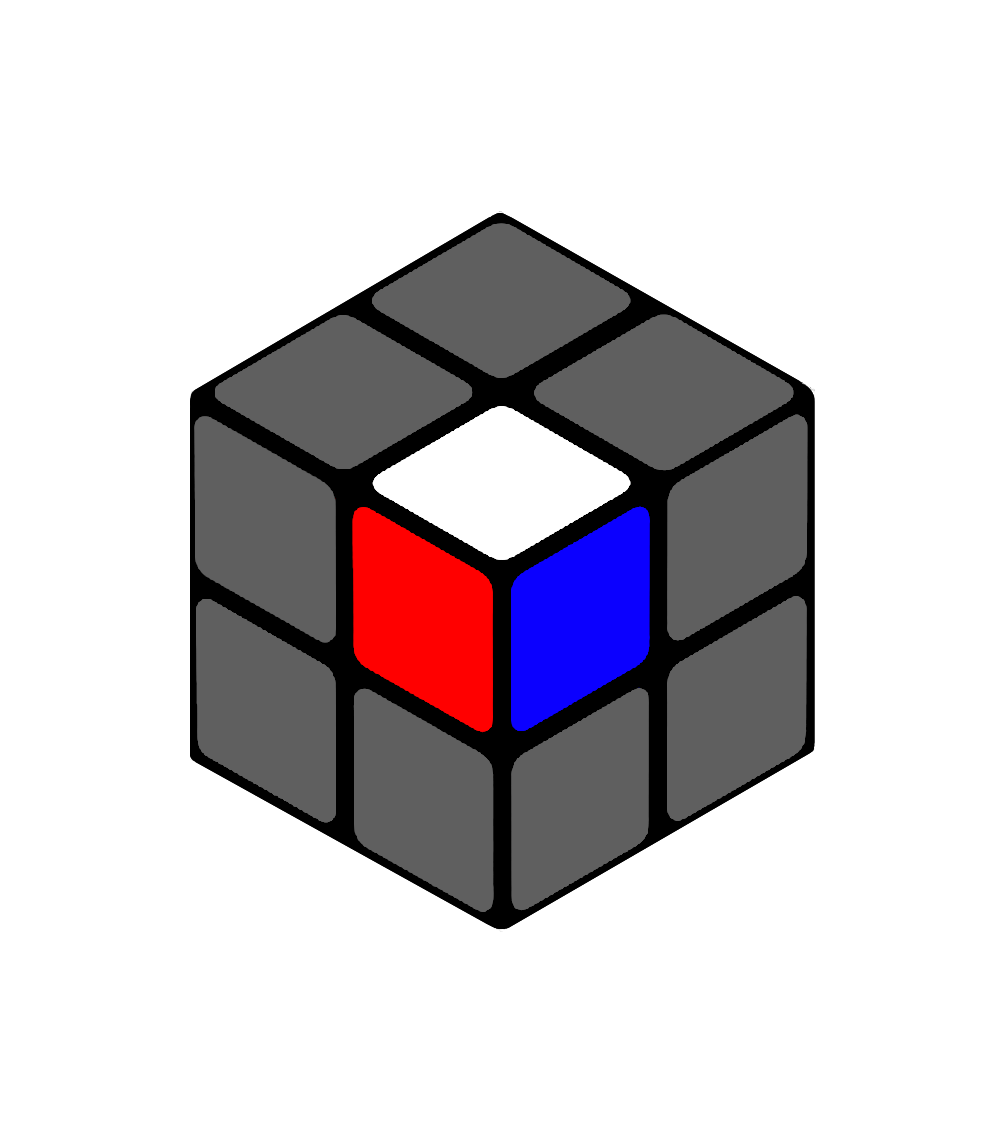
\includegraphics[scale=0.1]{2x2stein.png}
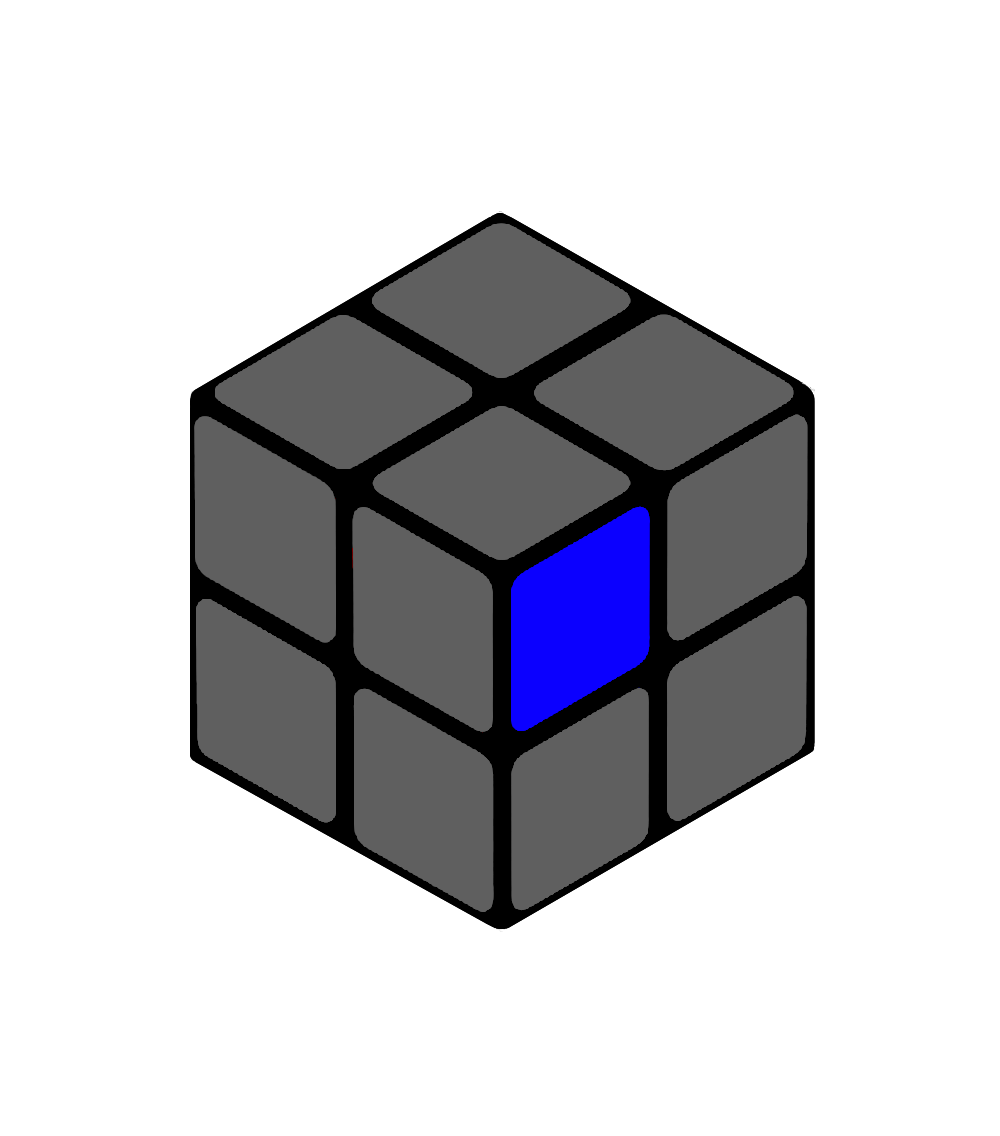
\includegraphics[scale=0.1]{2x2farbflaeche.png}
\caption[Eckstein und Farbfläche des Würfels]{Eckstein und Farbfläche des Würfels}
\label{Abbildung_Eckstein}
\end{figure} 


\newpage

\item[Seite] \ \\
Der \Ttwo und der \Tthree \ Würfel haben sechs Seiten (bestehend aus jeweils vier Farbflächen) und somit sechs Farben. Die weiße Seite wird üblicherweise als obere Seite bezeichnet. Für den Mechanismus ist die Ausrichtung des Würfels aber nicht relevant.

\begin{figure}[h]
\centering
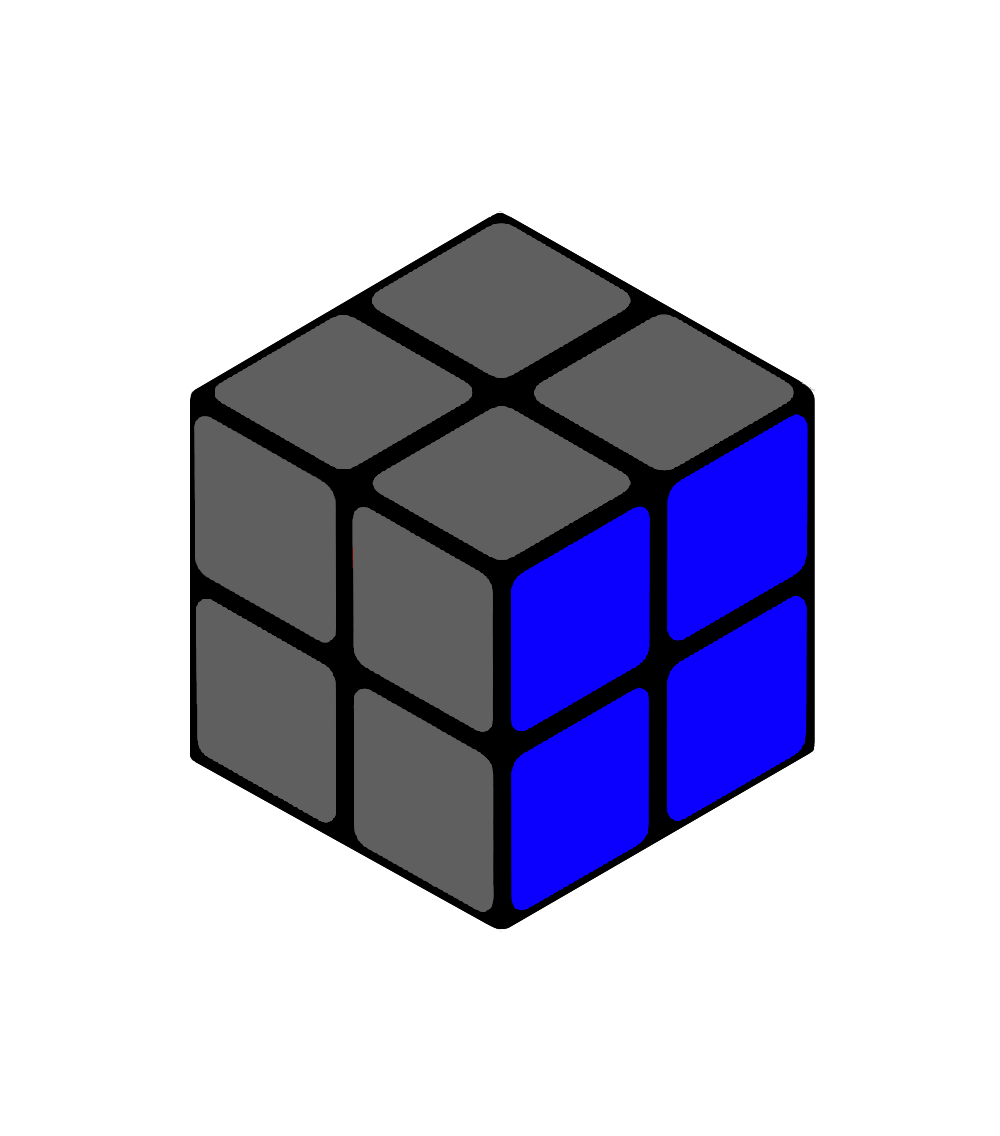
\includegraphics[scale=0.1]{2x2seite.png}
\caption[Seite des Würfels]{Seite des Würfels}
\end{figure}


\item[\Tthree Würfel] \ \\
Wesentlich bekannter als der \Ttwo \ ist der \Tthree Würfel. Er besteht aus 26 Steinen. In Abbildung \ref{Abbildung_3erWürfel} ist er links ungelöst und rechts in der Startkonfiguration zu sehen.

\begin{figure}[h]
\centering
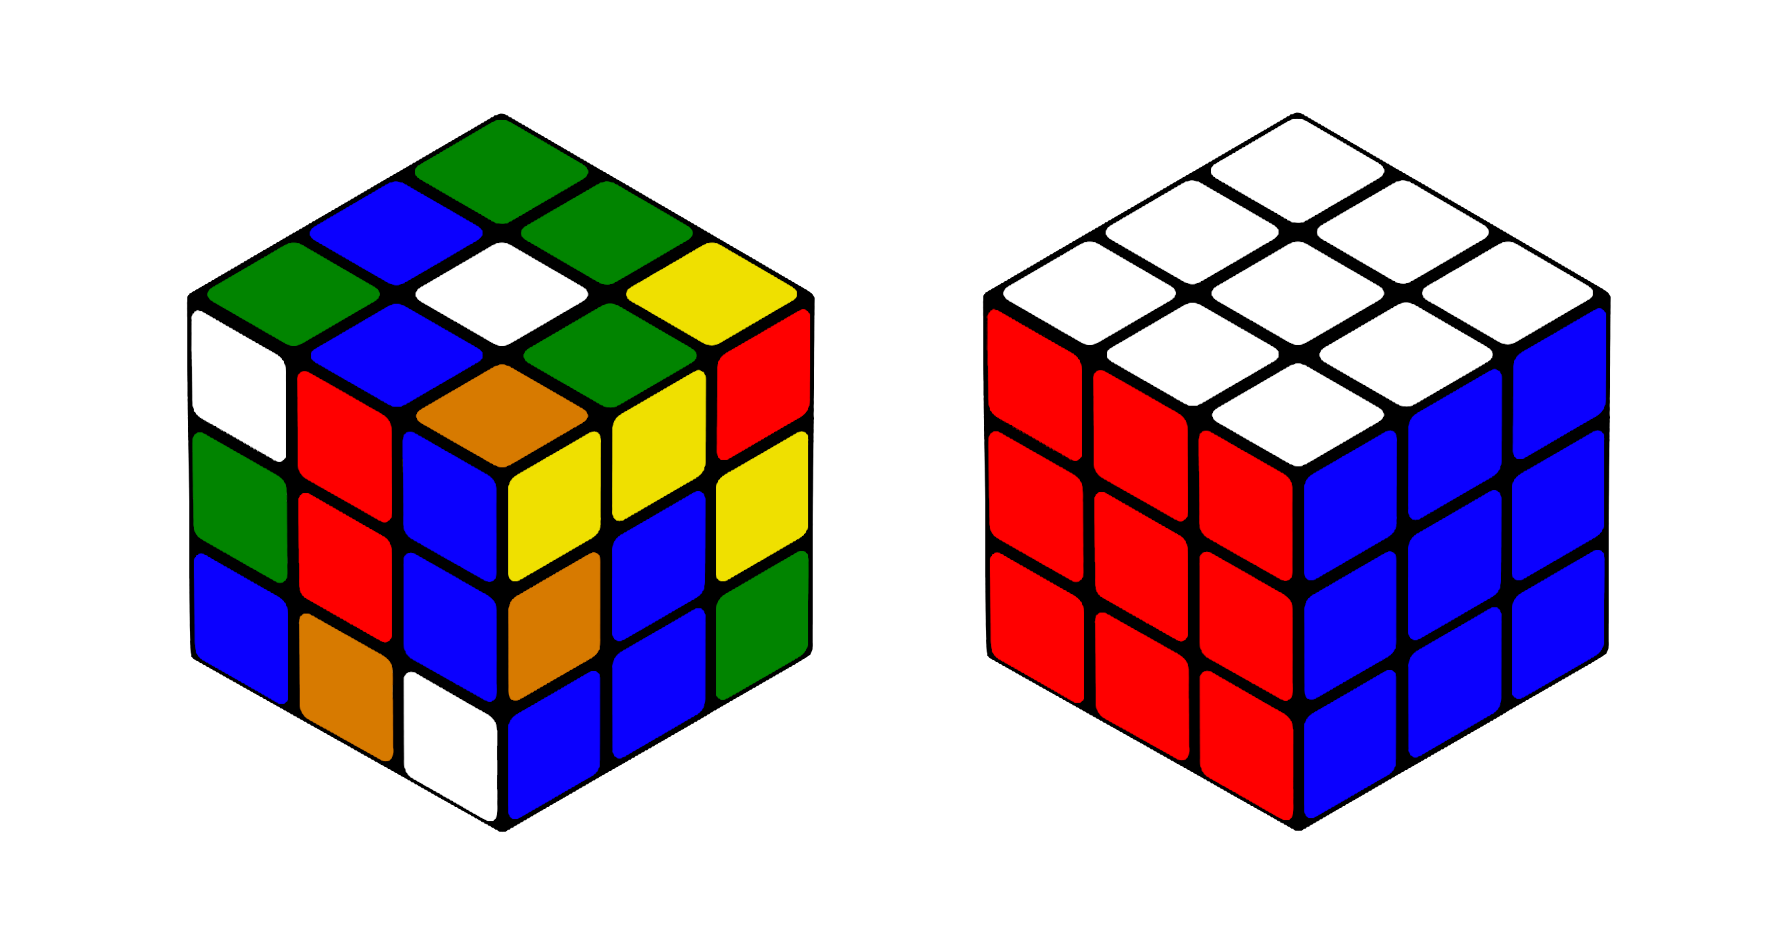
\includegraphics[scale=0.11]{3x3_sc_so.png}
\caption[Ungelöster und gelöster \Tthree Würfel]{Ungelöster und gelöster \Tthree Würfel}
\label{Abbildung_3erWürfel}
\end{figure}

\newpage
\item[Mittel- und Kantsteine] \ \\
Im Gegensatz zum \Ttwo \ hat der \Tthree Würfel Kantsteine und Mittelsteine (s. Abbildung \ref{Abbildung_MittelKantSteine}).
Das Besondere an den Mittelsteinen des \Tthree Würfels ist, dass sie bei Ebenendrehungen (also bei den Zügen des Würfels) nicht verändert werden. Somit ist beim \Tthree Würfel die obere Seite immer identifizierbar: Die obere Seite hat immer den weißen Mittelstein in der Mitte. 
\begin{figure}[H]
\centering
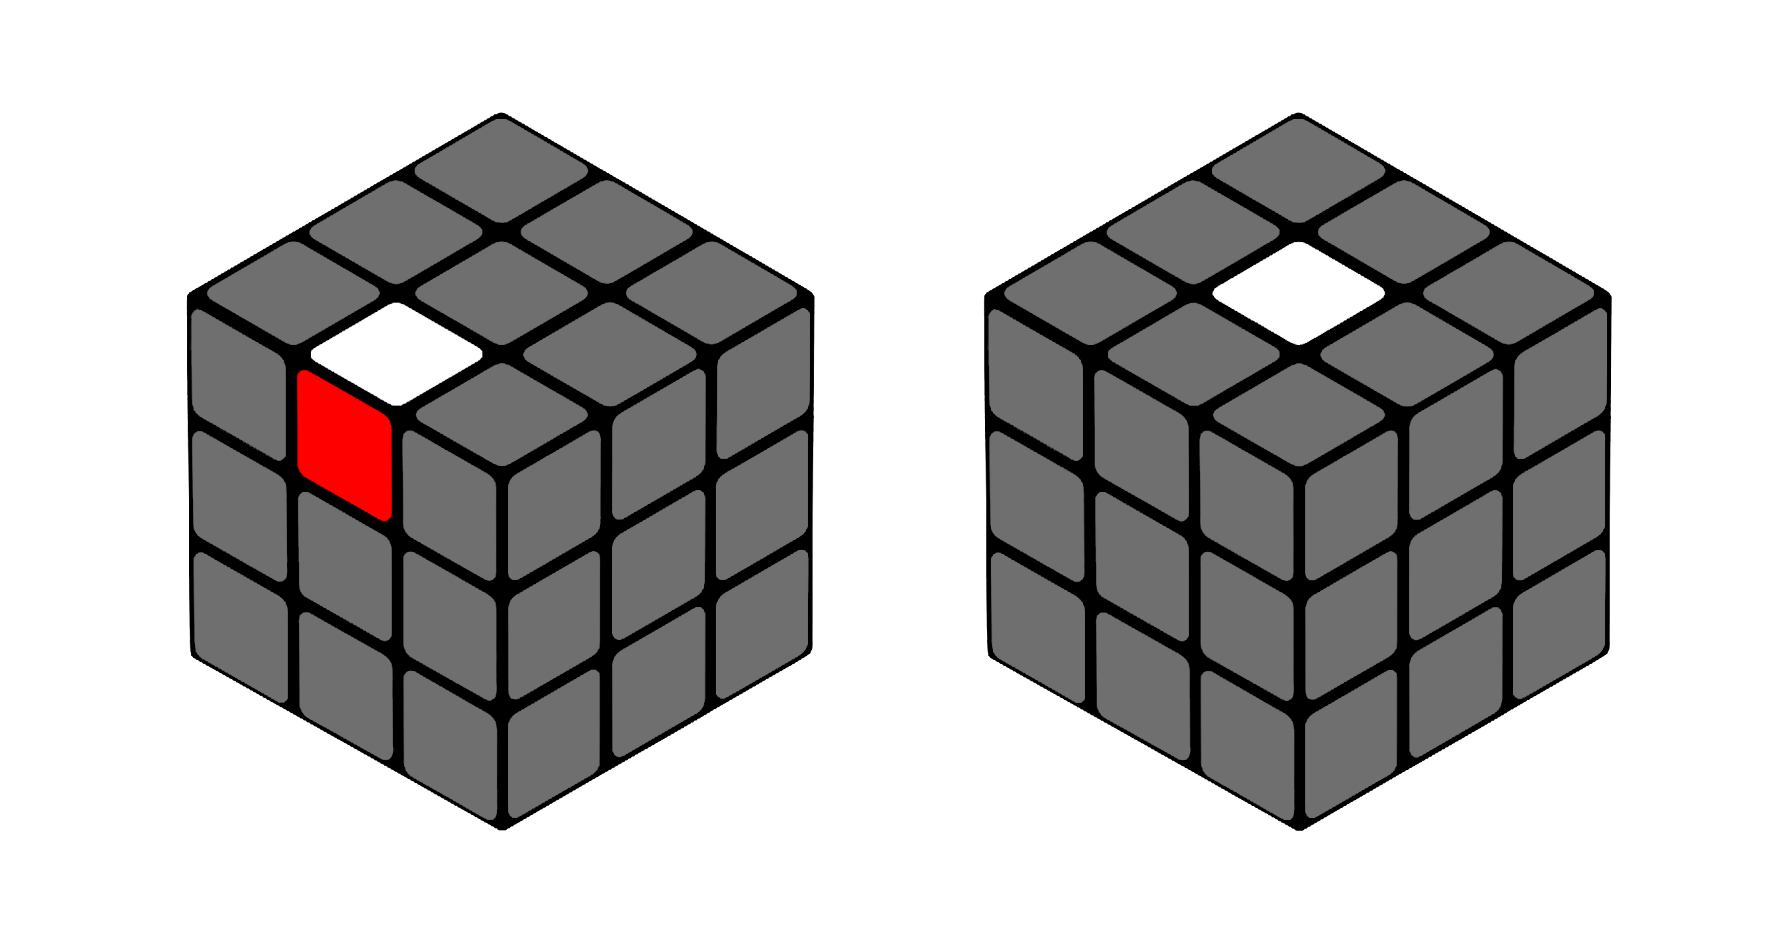
\includegraphics[scale=0.11]{mittelkant.png}
\caption[Kant- und Mittelsteine]{Kant- und Mittelsteine}
\label{Abbildung_MittelKantSteine}
\end{figure}



\end{description}

Beim \Ttwo \textit{Cube} gibt es keine eindeutige Oberseite. Es ist dementsprechend möglich, dass die aktuelle Würfelkonfiguration einer vermeintlich anderen Konfiguration entspricht, bei der jedoch eine andere Seite nach oben gehalten wird.
Die Ausrichtung des gesamten Würfels ist bei dem \Tthree Würfel also eindeutig vorgegeben, während sie beim \Ttwo Würfel gedreht werden kann.  
Dieser Sachverhalt ist entscheident bei der Übertragung der Gruppentheorie des \Tthree \textit{Cubes} auf den \Ttwo Würfel. Es wird sich dabei vorallem an \textit{Group Theory an the Rubik's Cube} von Janet Chen \cite{JC} und \textit{Group Theory via Rubik's Cube} von Tom Davis \cite{TD} orientiert.

%
%
%
%
%
%
%
%=======================================================================================================
%
%
%
%
%
%


\subsection{Grundzüge des Würfels} 

\label{Abschnitt_GrundzügeWürfel}
Am \Ttwo Zauberwürfel gibt es sechs verschiedene Drehseiten (auch Ebenen): oben, unten, links, rechts, vorne und hinten. 
In Abbildung \ref{Abbildung_Ebene} ist die obere Ebene markiert.

\begin{figure}[H]
\centering
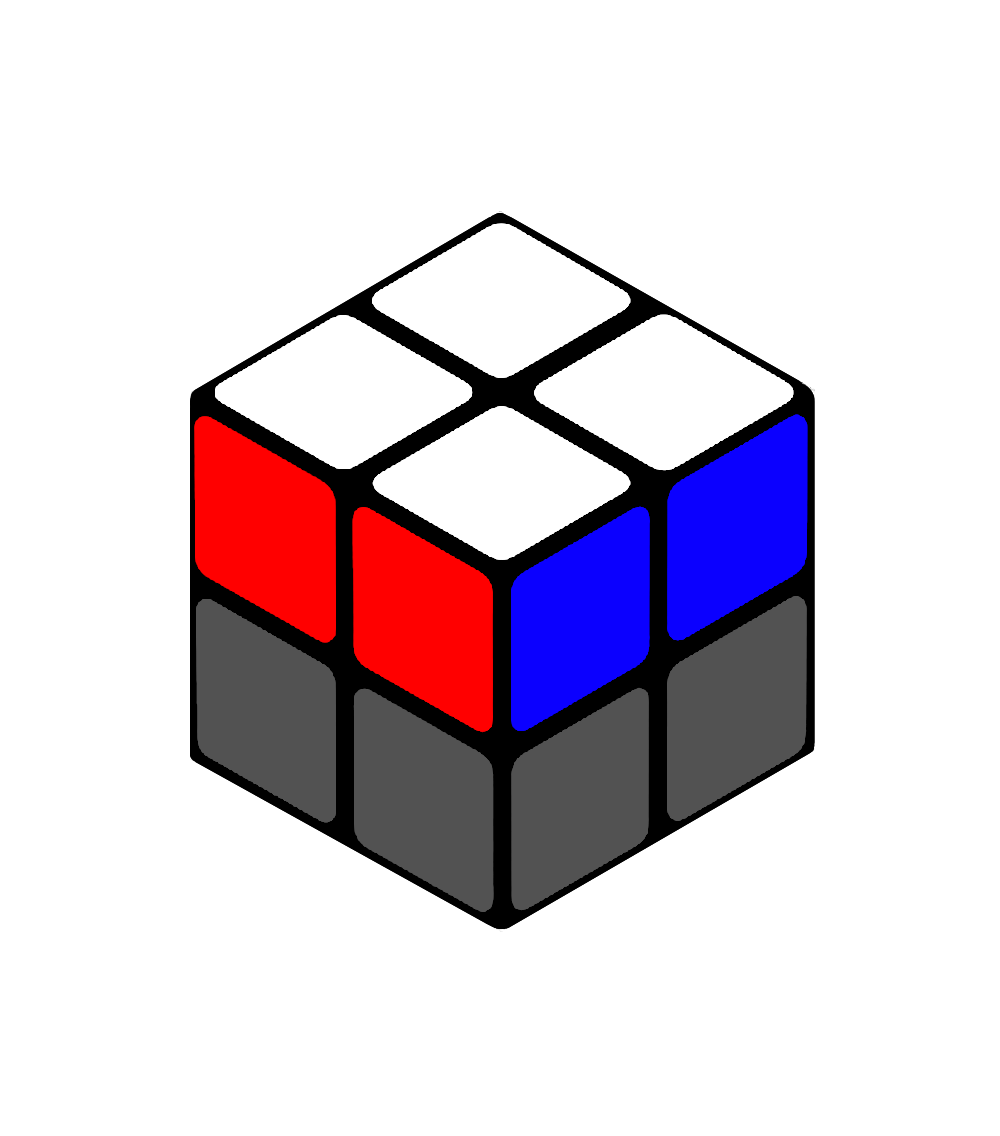
\includegraphics[scale=0.1]{ebene.png}
\caption[Ebene des Würfels]{Ebene des Würfels}
\label{Abbildung_Ebene}
\end{figure}

\begin{center}
\begin{tabular}{cl}
\toprule
\textbf{Abkürzung} & \textbf{Beschreibung des Zuges} \\
\midrule
$U$ & Drehung der \textbf{oberen} Ebene im Uhrzeigersinn \\
$D$ & Drehung der \textbf{unteren} Ebene im Uhrzeigersinn \\
$R$ & Drehung der \textbf{rechten} Ebene im Uhrzeigersinn \\
$L$ & Drehung der \textbf{linken} Ebene im Uhrzeigersinn \\
$F$ & Drehung der \textbf{vorderen} Ebene im Uhrzeigersinn \\
$B$ & Drehung der \textbf{hinteren} Ebene im Uhrzeigersinn \\
\bottomrule
\end{tabular} 
\end{center}

Die Kürzel stehen für \textit{Up, Down, Right, Left, Front, Back}. 
Die entsprechende Ebene wird um $90^\circ$ im Uhrzeigersinn gedreht, wenn auf diese Ebene geschaut wird. Dementsprechend wirkt es so, als würde die untere Ebene gegen den Uhrzeigersinn gedreht werden, wenn von oben auf den Würfel geschaut wird. So ergibt sich die Menge der Grundzüge: $\{U, D, R, L, F, B\}$.


Da der \Ttwo Würfel im Gegensatz zum \Tthree Würfel aber immer lediglich zwei statt drei nebeneinanderliegende Ebenen hat, entspricht eine Drehung der oberen Ebene nach rechts, einer Drehung der unteren Ebene nach links. 
Auf die Rotationsmöglichkeiten des kompletten Würfels wird in Abschnitt \ref{Abschnitt_RotationDesWürfels} genauer eingegangen. Trotzdem werden die Drehungen für jede Ebene definiert. Das ist zwar nicht minimal, dient aber der besseren Anschaulichkeit und Übertragbarkeit der Algorithmen.
Eine Drehung der oberen Ebene im Uhrzeigersinn ($U$) beispielsweise entspricht einer Drehung der unteren Ebene im Uhrziegersinn ($D$) mit anschließender Rotation des kompletten Würfels. Es ist aber übersichtlicher, jede Ebenendrehung als einzelnen Zug darzustellen. 

Eine minimale Menge der Grundzüge, die nicht voneinander ableitbar sind, ist $\{U, R, F\}$. Die minimale Abbildung des Würfels wird in Kapitel \ref{Kapitel_MinUntergruppe} behandelt.



%
%
%
%
%
%
%
%
%=======================================================================================================
%
%
%
%
%
%
%
%
%


\newpage
\section{Mathematische Grundlagen}

\label{Kapitel_MathematischeGrundlagen}

In diesem Kapitel werden die mathematischen Grundlagen erklärt, die für den weiteren Inhalt dieser Arbeit relevant sind. Es werden Definitionen und Beispiele von Gruppen, Untergruppen, zyklischen Gruppen, Erzeugern, Gruppenoperationen, Kommutatoren, Äquivalenzrelationen, Permutationen und der Zykelschreibweise angegeben.
Die genannten Definitionen basieren auf denen von Tobias Glosauer aus dem Buch \textit{Elementar(st)e Gruppentheorie} \cite{Buch}. Dort finden sich außerdem detailliertere Informationen und weitere Beispiele.
Des Weiteren wird der Cayleygraph erklärt. 
%
%
%
%=======================================================================================================
%
%
%
\subsection{Gruppe}
\label{Abschnitt_Gruppe}

\subsubsection*{Definition einer Gruppe}

Die Definition einer Gruppe $(G, \circ)$ ist Grundlage für die folgenden Kapitel. 

\begin{definition}[Gruppe]
Eine Menge $G$ (auch Trägermenge) mit einer Verknüpfung $\circ$ wird Gruppe genannt, wenn folgende Bedingungen gelten: 
\vspace*{-0.5em}
\begin{itemize}
\item Abgeschlossenheit: $\forall a,b \in G.(a \circ b) \in G $
\item Assoziativität: $\forall a,b,c \in G.(a \circ b) \circ c = a \circ (b \circ c)$
\item Existenz eines neutralen Elements $n$: $\exists n \in G. \forall a \in G.n \circ a = a \circ n = a$ 
\item Existenz eines inversen Elements $a^{-1}$: $\forall a \in G. \exists a^{-1} \in G. a \circ a^{-1} = a^{-1} \circ a = n$ 
\end{itemize}
\end{definition}

Wenn es sich bei der Gruppe um eine kommutative Gruppe (auch abelsche Gruppe\footnote{\glqq Zu Ehren von Niels Henrik \textsc{Abel} (1802-1829); norwegischer Mathematiker und einer der Begründer der Gruppentheorie. Starb leider verarmt und deprimiert im Alter von 26 Jahren an Tuberkulose, kurz bevor er als Anerkennung für seine genialen Arbeiten  eine Dozentenstelle in Berlin angeboten bekam.\grqq \  \cite[S.21, Z.23]{Buch}}) handelt, muss zusätzlich noch die Eigenschaft der Kommutativität gelten: 

\begin{definition}[Kommutative Gruppe]
Eine Gruppe $(G, \circ)$ ist eine kommutative Gruppe, wenn gilt:
\vspace*{-0.5em}
\begin{itemize}
\item Kommutativität: $\forall a,b \in G.(a \circ b) = (b \circ a) $
\end{itemize}
\end{definition}
\vspace*{0.1cm}


\begin{bsp}[Gruppe]

Zur Veranschaulichung der Gruppendefinition werden hier die natürlichen Zahlen $\mathbb{N}$ und die ganzen Zahlen $\mathbb{Z}$ mit dem Operator $+$ auf die Gruppenaxiome untersucht.
\begin{itemize}
\item Die Abgeschlossenheit gilt sowohl für $(\mathbb{N},+)$ als auch für $(\mathbb{Z},+)$, da zwei natürliche Zahlen addiert immer eine natürliche Zahl ergeben. Zwei ganze Zahlen addiert ergeben immer eine ganze Zahl. \\
Beispielsweise sind $1+2=3$ und es gilt $1,2,3 \in \mathbb{N}$.
\item Die Verknüpfung ist assoziativ, aufgrund der Definition des Pluszeichens.
\item Das neutrale Element von $(\mathbb{N},+)$ und $(\mathbb{Z},+)$ ist $0$. Es gilt also $\forall n \in N. \ n + 0 = 0 + n = n$ (und mit $\mathbb{Z}$ analog). \\
Ein Beispiel zur Veranschaulichung: $3+0=0+3=3$
\item Die letzte erforderliche Eigenschaft einer Gruppe ist die Existenz eines inversen Elements. Für die Gruppe $(\mathbb{Z},+)$ ist $-z$ das inverse Element für jedes $z \in \mathbb{Z}$. Für $(\mathbb{N},+)$ gibt es kein inverses Element.
\end{itemize}
Anhand der oberen Axiome kann nun festgestellt werden, dass $(\mathbb{Z},+)$ die Gruppeneigenschaften erfüllt, $(\mathbb{N},+)$ aber nicht. 
$(\mathbb{Z},+)$ ist folglich eine Gruppe und $(\mathbb{N},+)$ nicht, da kein inverses Element existiert. 
Es ist aber zu beachten, dass es sich hierbei nicht um formelle Beweise, sondern um anschauliche Beschreibungen handelt.
Nun kann $(\mathbb{Z},+)$ noch auf die Kommutativität untersucht werden, um zu prüfen, ob es sich um eine abelsche Gruppe handelt. \\
Da der Plus-Operator als kommutativ definiert ist, ist $(\mathbb{Z},+)$ eine abelsche Gruppe.

\end{bsp}

\begin{bsp}[Gruppe]

Beispiele für endliche Gruppen sind die zyklischen Gruppen der Form $\mathbb{Z}_{\hspace*{-0.3em}\mod n}$. Hier wird die Menge für $n=6$ mit dem Additionsoperator auf die Gruppeneigenschaften untersucht. Die Elemente der Menge sind dann alle ganzen Zahlen modulo 6, also $\mathbb{Z}_{\hspace*{-0.3em}\mod 6}=\{0,1,2,3,4,5\}$
\begin{itemize}
\item Die Abgeschlossenheit gilt für $(\mathbb{Z}_{\hspace*{-0.3em}\mod 6}, +)$, da alle Elemente aus $\mathbb{Z}$ nach der Anwendung von$\mod 6$ in der Menge $\{0,1,2,3,4,5\}$ liegen.
\item Die Verknüpfung ist assoziativ, da das Pluszeichen so definiert ist.
\item Das neutrale Element von $(\mathbb{Z}_{\hspace*{-0.3em}\mod 6}, +)$ ist $0$.
\item Das Inverse Element für alle $z \in \mathbb{Z}_{\hspace*{-0.3em}\mod 6}$ ist definiert als $(6-z)$. Für 1 ist es demnach 5, für 2 ist es 4 und für 3 ist das inverse Element die 3.
\end{itemize}

$(\mathbb{Z}_{\hspace*{-0.3em}\mod 6}, +)$ ist eine endliche Gruppe, da die vier Gruppeneigenschaften erfüllt sind und die Trägermenge $\mathbb{Z}_{\hspace*{-0.3em}\mod 6}$ endlich ist.

\end{bsp}

\subsubsection*{Mächtigkeit einer Gruppe}

\label{Abschnitt_MächtigkeitGruppe}

Die Mächtigkeit einer Gruppe $(G, \circ)$ wird auch Gruppenordnung genannt und sagt aus, wie viele Elemente die Menge $G$ der Gruppe enthält.

\begin{definition}[Mächtigkeit einer Gruppe]
Die Mächtigkeit einer Gruppe $(G, \circ)$ ist der Betrag der Menge $G$, also $|G|$. 
\end{definition}

Wenn $|G| < \infty$, wird von einer endlichen Gruppe gesprochen.

\begin{bsp}[Mächtigkeit einer endlichen Gruppe]

Die Mächtigkeit der Gruppe $(\mathbb{Z}_{\hspace*{-0.3em}\mod 6}, +)$ ist $6$. Die Menge $\mathbb{Z}_{\hspace*{-0.3em}\mod 6}$ enthält die Elemente $\{0,1,2,3,4,5 \}$ und somit ist $| \mathbb{Z}_{\hspace*{-0.3em}\mod 6} | = 6$.

\end{bsp}

\begin{bsp}[Mächtigkeit einer unendlichen Gruppe]

Die Mächtigkeit der Gruppe $(\mathbb{Z}, +)$ ist $\infty$, da $|\mathbb{Z}|$ (abzählbar) unendlich ist.

\end{bsp}

%
%
%
%
%
%=======================================================================================================
%
%
%
%
%
\subsection{Untergruppe} 
\label{Abschnitt_Untergruppe}

Im Folgenden werden Untergruppen definiert.


\begin{definition}[Untergruppe]
Eine Gruppe $(H, \circ)$ ist eine Untergruppe einer Gruppe $(G, \circ)$, wenn $H \subseteq G$ gilt. Dann wird auch $(H, \circ) \leqslant (G, \circ)$ geschrieben. 
\end{definition}

Das Symbol $\leqslant$ ist zu lesen als \textit{ist Untergruppe von}. Nicht jede Teilmenge $H \subseteq G$ muss Trägermenge einer Gruppe sein.

Wenn $(H, \circ)$ eine Untergruppe der Gruppe $(G, \circ)$ ist, wird $(G, \circ)$ auch Obergruppe von $(H, \circ)$ genannt.
Jede Gruppe $(G, \circ)$ mit neutralem Element $N$ hat die beiden trivialen Untergruppen $(H_N, \circ)$ mit ${H_N = \{N\}}$ und $(H_G, \circ)$ mit $H_G=G$.


\begin{bsp}[keine Untergruppe]

Bei dem oben genannten Beispiel mit $(\mathbb{N},+)$ und $(\mathbb{Z},+)$ stellt sich heraus, dass $(\mathbb{Z},+)$ eine Gruppe ist und $(\mathbb{N},+)$ nicht. Obwohl $\mathbb{N \subseteq \mathbb{Z}}$, ist $(\mathbb{N},+)$ \textit{keine} Untergruppe von $(\mathbb{Z},+)$, da die Gruppeneigenschaft \textit{Existenz eines inversen Elements} nicht erfüllt sind.

\end{bsp}
\begin{bsp}[Untergruppe]

Es gilt $\mathbb{Z}_{\hspace*{-0.3em}\mod 6} \subseteq \mathbb{Z}$. Da sowohl $(\mathbb{Z},+)$, als auch $(\mathbb{Z}_{\hspace*{-0.3em}\mod 6}, +)$ Gruppen sind, ist $(\mathbb{Z}_{\hspace*{-0.3em}\mod 6}, +)$ eine Untergruppe von $(\mathbb{Z},+)$. $(\mathbb{Z}_{\hspace*{-0.3em}\mod 6}, +)$ und $(\mathbb{Z},+)$ wurden im Abschnitt über Gruppen auf die Gruppeneigenschaften untersucht.

\end{bsp}

%
%
%
%
%
%=======================================================================================================
%
%
%
%
%

\subsection{Erzeuger und zyklische Gruppe} 
\label{Abschnitt_Erzeuger}


\begin{definition}[Erzeuger]
Sei die Menge $M \subseteq G$ eine nicht leere Teilmenge der Trägermenge einer Gruppe $(G, \circ)$. 
Dann wird die Untergruppe $(M, \circ)$ von $M$ erzeugt und ist die kleinste Untergruppe von $(G, \circ)$, für die $M \subseteq G$ gilt.
$(M, \circ)$ wird dann Erzeugnis von $M$ genannt und die Elemente aus $M$ sind die Erzeuger der Untergruppe $(M, \circ)$.
\end{definition}

Eine zyklische Gruppe ist eine Gruppe, die von nur einem Element erzeugt wird. Sie besteht ausschließlich aus Potenzen dieses Elementes

\begin{definition}[Zyklische Gruppe]
Sei $(G, \circ)$ eine Gruppe. $(G, \circ)$ wird zyklische Gruppe genannt, wenn es ein Element $a \in G$ gibt, das jedes Element in $G$ erzeugt. Dann schreibt man auch:
\begin{align*}
\langle a \rangle := \{ a^n \mid n \in \mathbb{Z} \}
\end{align*}

\end{definition}


\begin{bsp}[Erzeuger und zyklische Gruppe]

Ein Beispiel für Erzeuger findet sich anhand der Gruppe der ganzen Zahlen $(\mathbb{Z},+)$ und der Addition als Verknüpfung, die bereits als Beispiel der Gruppe beschrieben wurde.

Die Operationen sind hier die Addition und der Übergang von einer Zahl $z$ zu der negativen Zahl $-z$.

Ein Erzeuger dieser Gruppe ist die einelementige Menge $M = \{ 1 \}$. Jede positive Zahl $n$ lässt sich durch die $n$-fache Addition von $1$ erzeugen und jede negative Zahl durch  die Addition von $((-1)+(-1)...)$. 

\end{bsp}
%
%
%
%
%=======================================================================================================
%
%
%
%
%
\subsection{Cayleygraph} 
\label{Abschnitt_Cayleygraph}
Ein Cayleygraph ist ein Graph, der die Struktur einer Gruppe beschreibt. Er hängt von der Menge der Erzeuger ab und dient dazu, Gruppen bildlich darzustellen.
Es handelt sich dabei um einen Graphen mit Knoten, die die verschiedenen Gruppenelemente darstellen. Pfeile zeigen von einem Element zum nächsten, wenn dies durch einen der Erzeuger erreicht werden kann. \cite{AT}

\textbf{Beispiel} (Cayleygraph) \\
In Abbildung \ref{Abbildung_Cayleygraph} ist der Cayleygraph der Gruppe $(\mathbb{Z}_{\hspace*{-0.3em}\mod 6}, +)$ mit dem Erzeuger $1$ dargestellt.

\begin{figure}[H]
\centering
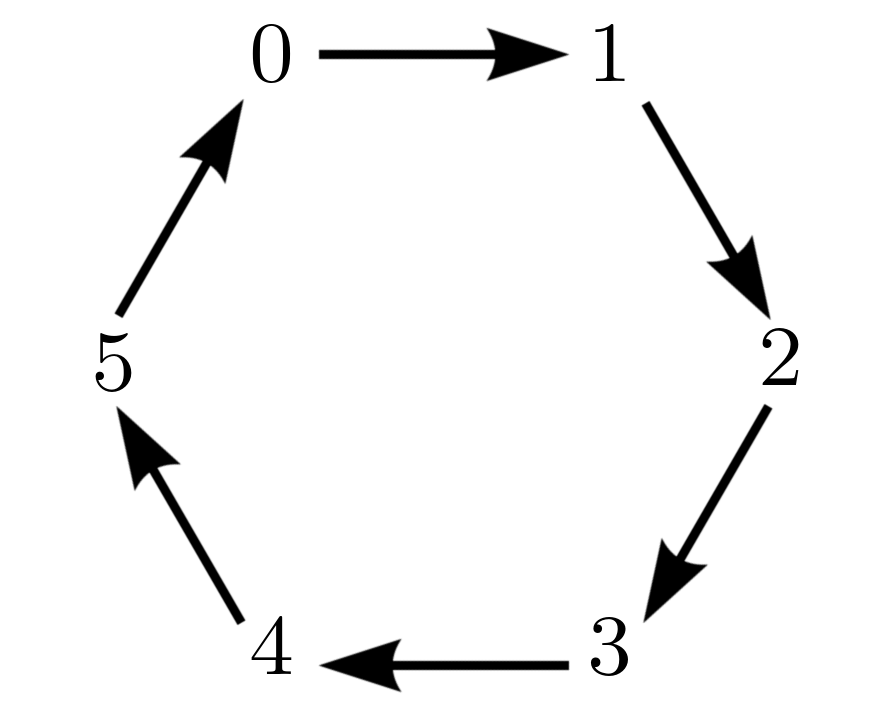
\includegraphics[scale=0.7]{Cayleygraph3.png}
\caption{Cayleygraph von $(\mathbb{Z}/6\mathbb{Z}, +)$ mit Erzeuger $1$}
\label{Abbildung_Cayleygraph}
\end{figure}


%
%
%
%
%=======================================================================================================
%
%
%
%
%
%

\subsection{Gruppenoperation}
 \label{Abschnitt_Gruppenoperation}



Es gibt Links- und Rechtsoperationen auf Gruppen. Da in dieser Arbeit ausschließlich Rechtsoperationen genutzt werden, beschränkt sich die Definition darauf.


\begin{definition}[Rechtsoperation]

Eine Rechtsoperation einer Gruppe $(G, \circ)$ auf einer Menge $M$ ist eine Verknüpfung mit $m \in M$, $e$ als neutralem Element von $(G,\circ)$ und $g,h \in G$:
\begin{align*}
\cdot: M \times G \rightarrow M \ \ \ \ \ \ \ \ \ \ \ \ \ \ \
(m, g) \mapsto m \cdot g 
\end{align*}
Die folgenden beiden Eigenschaften gelten:
\begin{align*}
m \cdot e & = m \\
m \cdot (g \circ h) & = (m \cdot g) \cdot h
\end{align*}
Dann operiert $G$ von rechts auf $M$.

\end{definition}


\begin{bsp}[Rechtsoperation]

Als Beispiel werden die Gruppe $(\mathbb{Z}_{\hspace*{-0.3em}\mod 6}, +)$ und die Menge $\mathbb{Z}$ mit der Verknüpfung $-$ betrachtet. Die folgenden Eigenschaften gelten, da $(\mathbb{Z}_{\hspace*{-0.3em}\mod 6}, +)$ eine Rechtsoperation auf $\mathbb{Z}$ ist, mit $z \in  \mathbb{Z}$ und $g,h \in \mathbb{Z}_{\hspace*{-0.3em}\mod 6}$.
\begin{itemize}
\item Die Eigenschaft $z - 0 = z$ ist erfüllt. $0$ ist das neutrale Element von $(\mathbb{Z}_{\hspace*{-0.3em}\mod 6}, +)$.
\item Da sich $z-(g+h)$ zu $z-g-h$ umformen lässt, gilt $z-(g+h) = (z-g)-h$
\end{itemize}
Demnach operiert $(\mathbb{Z}_{\hspace*{-0.3em}\mod 6}, +)$ mit $-$ von rechts auf $\mathbb{Z}$.

\end{bsp}

%
%
%
%
%
%=======================================================================================================
%
%
%
%
%
%
%

\subsection{Kommutator} 
 \label{Abschnitt_Kommutator}
Die Komplexität eines Kommutators sagt etwas darüber aus, wie stark zwei Elemente einer Gruppe das Kommutativgesetz verletzen. Bei kommutativen Gruppen ist der Kommutator zweier Elemente das neutrale Element der Gruppe \cite{TD}. Man sagt dann, dass die beiden Elemente kommutieren. 


\begin{definition}[Kommutator]
Als Kommutator von zwei Elementen $a, b$ einer Gruppe $(G, \circ)$  bezeichnet man $[a,b] = aba^{-1}b^{-1}$.
\end{definition}


\begin{bsp}[Kommutator]

$[5,7]$ ist ein Kommutator der Gruppe $(\mathbb{Z}, +)$. $[5,7]$ entspricht $5+7-5-7 = 0$ und $0$ ist das neutrale Element der Gruppe. Die Gruppe $(\mathbb{Z}, +)$ ist kommutativ, deshalb ist der Kommutator von allen Elementen der Gruppe $0$.

\end{bsp}
%
%
%
%
%
%
%=======================================================================================================
%
%
%
%
%
%
%

\subsection{Äquivalenzrelation und -klasse}

 
\subsubsection*{Äquivalenzrelation}

 \label{Abschnitt_Äquivalenrelationen}

Mit Relationen lassen sich Beziehungen von Elementen einer Menge zueinander beschreiben.

\begin{definition}[Äquivalenzrelation]
Eine Relation $\sim \ \subseteq A \times A$ heißt Äquivalenzrelation auf $A$, wenn für alle $x, y, z \in A$ die drei folgenden Eigenschaften gelten: Reflexivität, Symmetrie, Transitivität.
\end{definition}


Hier wird $x \sim y$ als \textit{x ist äquivalent zu y} gelesen. Im Folgenden werden noch die Bedeutungen von Reflexivität, Symmetrie und Transitivität aufgelistet:

\begin{center}
\begin{tabular}{ll}
$x \sim x$ & (Reflexivität) \\
Aus $(x \sim y)$ folgt $(y \sim x)$. & (Symmetrie) \\
Aus $(x \sim y)$ und $(y \sim z)$ folgt $(x \sim z)$. & (Transitivität) \\
\end{tabular}
\end{center}


\begin{bsp}[Relation]


Für die Menge $A=\{ 1, 2, 3, 4, 5 \}$ wird die Relation $ x < y$ betrachtet:

Bei der Relation $< $ handelt es sich nicht um eine Äquivalenrelation, da die Eigenschaft der Reflexivität nicht gilt: $1 \nless 1$. Auch die Symmetrie gilt nicht.


\end{bsp}
\begin{bsp}[Äquivalenzrelation]
Für die Menge $A=\{ 1, 2, 3, 4, 5 \}$ wird die Relation $ x = y$ betrachtet:

Bei der Relation $=$ gilt die Reflexivität für alle Elemente, da ein Element immer mit sich selbst identisch ist. Auch die Symmetrie und die Transitivität gelten für die Gleichheit. Somit ist es eine Äquivalenzrelation. 


\end{bsp}

\begin{bsp}[Äquivalenzrelation]
Für die Menge $A=\{ -3, -2, -1, 0, 1, 2, 3 \}$ wird die Relation $x \sim_+ y$ betrachtet, die als $|x| =|y|$ definiert ist:

Bei der Relation $\sim_+$ gilt die Reflexivität für alle Elemente, da die Gleichheit reflexiv ist. Auch die Symmetrie und die Transitivität gelten für die Gleichheit mit Betrag. Somit ist es eine Äquivalenzrelation. 


\end{bsp}

\subsubsection*{Äquivalenzklasse und Faktormenge} 
\label{Abschnitt_FaktormengenUndÄquivalenzklasse}

Äquivalenzklassen sind Mengen, die äquivalente Elemente enthalten.

\begin{definition}[Äquivalenzklassen]

Sei $ \sim $ eine Äquivalenzrelation auf der Menge $M$ und $x \in M$. Die Äquivalenzklasse von $x$ wird dann als $[x]$ geschrieben und ist definiert als $\{y \in M \mid y \sim x\} \subseteq M$.  

\end{definition}

Jedes Element der Äquivalenzklasse $[x]$ heißt \textit{Repräsentant von $[x]$}. Alle Repräsentanten von $[x]$ sind äquivalent zu $x$.

\begin{bsp}[Äquivalenzklassen]
Es wird die Äquivalenzrelation $x \sim_+ y$, die als $|x| =|y|$ definiert ist, auf der Menge $A=\{ -3, -2, -1, 0, 1, 2, 3 \}$ betrachtet. Die Äquivalenzklasse von $[1]$ beispielsweise ist dann $[1] = \{x \in A \mid x \sim_+ 1\}$. $[1]$ enthält dann die Elemente $1$ und $-1$.

\end{bsp}

\begin{definition}[Faktormenge]

Die Faktormenge $M / \sim $ der Menge $M$ bezüglich der Äquivalentionrelation $\sim$ besteht aus allen Äquivalentzklassen und ist definiert als $\{ [x] \mid x \in M \}$.

\end{definition}

$M / \sim $ wird als \textit{$M$ modulo $\sim$} gelesen. Die Elemente von $M / \sim $ sind Äquivalenzklassen.

\begin{bsp}[Faktormenge]

Es wird wieder die Äquivalenzrelation $x \sim_+ y$, die als $|x| =|y|$ definiert ist, auf der Menge $A=\{ -3, -2, -1, 0, 1, 2, 3 \}$ betrachtet.  \\
Die Faktormenge $A / \sim_+$ enthält dann die Äquivalenzklassen $[1]$, $[2]$, $[3]$ und $[0]$. $A / \sim_+$ also vier Elemente, während $A$ sieben Elemente hat.

\end{bsp}



%
%
%
%
%
%
%=======================================================================================================
%
%
%
%
%
%
%
\subsection{Permutationen und Zykelschreibweise} 
 \label{Abschnitt_PermutationZykel}

Unter einer Permutation versteht man die Vertauschung der Reihenfolge von Objekten.

\begin{definition}[Permutation]
Bei einer $n$-elementigen Menge $M$ ist eine ($n$-stellige) Permutation eine bijektive Abbildung $\pi  : M \rightarrow M$.
\end{definition}
Die Zykelschreibweise ist eine kurze Schreibweise für eine Permutation.
Die Zykelschreibweise wird nun anhand eines Beispiels erklärt. Die Definition geht über den Rahmen dieser Arbeit hinaus, sie kann aber in dem Buch \textit{Elementar(st)e Gruppentheorie} von Tobias Glosauer \cite{Buch} nachgelesen werden.

\begin{bsp}[Permutationen und Zykelschreibweise]
Sei $M$ eine Menge mit fünf Objekten: $1, 2, 3, 4$ und $5$. Nun können diese Objekte in fünf Plätzen arrangiert werden. Die Plätze werden mit $1$ bis $5$ nummeriert. Dann kann eine Funktion $\pi :\{1,2,3,4,5\} \rightarrow \{1,2,3,4,5\}$ definiert werden, bei der $\pi (i)$ die Zahl ist, die in Slot $i$ liegt.
Wenn die Zahlen in der Reihenfolge $5 \ 1\ 4\ 3 \ 2$ amgeordnet werden, ist $5$ auf Platz $1$, $1$ auf Platz $2$, usw. Das ist auch in der folgenden Tabelle zu sehen: 

\begin{center}
\begin{tabular}{l ccccc}

Platz & 1 & 2 & 3 & 4 & 5 \\
\midrule
Zahl & 5 & 1 & 4 & 3 & 2 \\

\end{tabular}
\end{center}

Die Funktion $\pi$ sieht für diese Permutation (s. Tabelle) so aus:
\begin{align*}
\pi(1) = 5 \ \ \ \ \ \  \pi(2) = 1 \ \ \ \ \ \ \pi(3) = 4 \ \ \ \ \ \ \pi(4) = 3 \ \ \ \ \ \ \pi(5) = 2 
\end{align*}
$\pi$ kann auch als eindeutige Zuordnung der Form $i \mapsto j$ (für $\pi(i)=j$) geschrieben werden, da jede Permutationsfunktion in dieser Form angegeben werden kann \cite{JC}:
\begin{align*}
1 \mapsto 5 \ \ \ \ \ \ \ \ \ \  2\mapsto 1 \ \ \ \ \ \ \ \ \ \ 3\mapsto 4 \ \ \ \ \ \ \ \ \ \ 4\mapsto 3 \ \ \ \ \ \ \ \ \ \ 5\mapsto 2 
\end{align*}
Das kann folgendermaßen in der Zykelschreibweise geschrieben werden:
\begin{align*}
\pi = (1 \ 5 \ 2)\ (3 \ 4)
\end{align*}
Das wird so gelesen: Die 1 geht auf die 5, die 5 geht auf die 2, die 2 geht wieder auf die 1. Damit ist der erste Zykel geschlossen. Beim zweiten Zykel geht die 3 auf die 4 und die 4 auf die 3. $\pi$ besteht somit aus zwei Zykeln: ein Zykel hat die Länge drei und der andere die Länge zwei. Die Zykel sind in Abbildung \ref{Abbildung_ZykelVonf} dargestellt.
\begin{figure}[H]
\centering
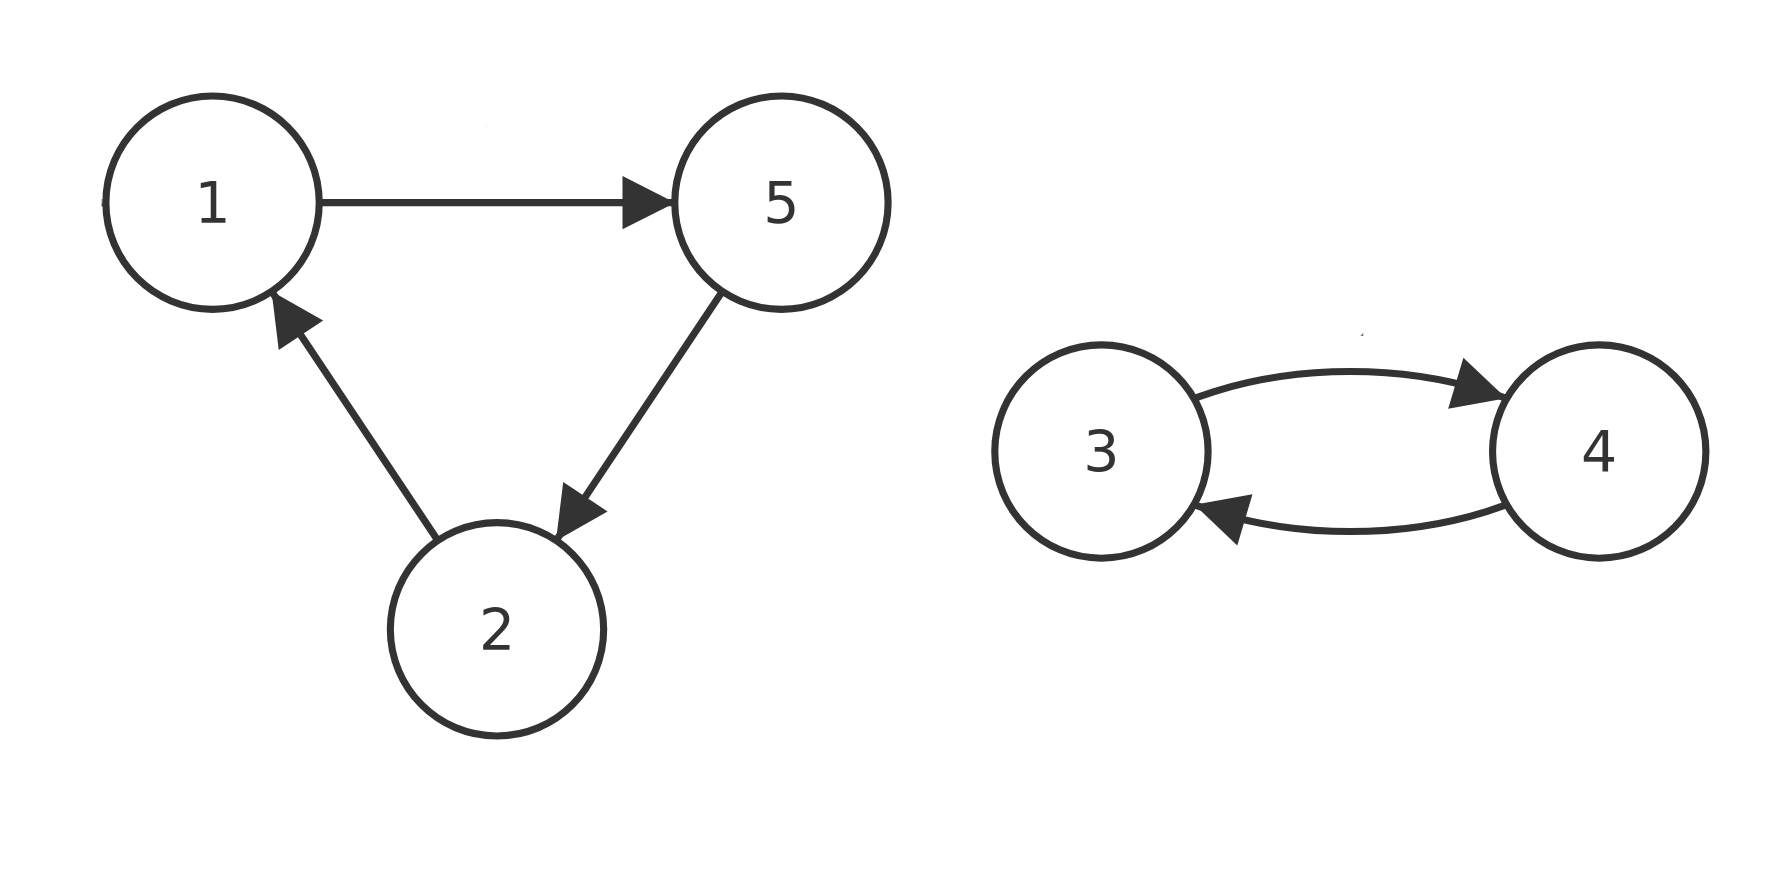
\includegraphics[scale=0.13]{Zykel_152.png}
\caption{Zykel $\pi = (1 \ 5 \ 2)\ (3 \ 4)$}
\label{Abbildung_ZykelVonf}
\end{figure}
Bei der Zykelschreibweise ist die Reihenfolge der Elemente ausschlaggebend. Beispielsweise ist $(1 \ 2 \ 3)$ nicht das gleiche wie $(1 \ 3 \ 2)$. 

Die Identitätspermutation wird als $\pi = 1$ geschrieben. Dabei werden alle Elemente auf sich selbst abgebildet und die Zykel bleiben somit unverändert.
\end{bsp}

\begin{definition}[Anzahl der Permutationen]
Für $n$ verschiedene Objekte ist die Anzahl der Permutationen $n!$.
\end{definition}

\begin{bsp}[Anzahl der Permutationen]
Sei $M = \{ 1 \ 2 \ 3 \}$ eine Menge mit drei Elementen. Für das erste Objekt der Permutation gibt es $3$ Möglichkeiten der Platzeinname: $1$, $2$ oder $3$. Für das zweite Objekt bleiben dann noch $2$ Möglichkeiten (da eine ja bereits im ersten Schritt eliminiert wurde) und danach gibt es nur noch eine Option. Es gibt dann also $3 \cdot 2 \cdot 1 = 3! = 6$ Permutationsmöglichkeiten.

\end{bsp}

\begin{definition}[Ordnung von Permutationen]

Die Ordnung einer Permutation ist das kleinste gemeinsame Vielfache der Zykellängen (kurz: kgV).

\end{definition}

Die Ordnung einer Permutation ist die kleinste Zahl $n \in \mathbb{N}$, so dass sich nach $n$-facher Ausführung der Permutation die identische Permutation ergibt. Man kann die Ordnung einer Permutation $\pi$ als \textit{ord}$(\pi)$ schreiben.

\begin{bsp}[Ordnung von Permutationen]

Sei die Permutation $\pi = (1 \ 2 \ 3)$. Die Ordnung von $\pi$ ist 3, da $\pi$ aus nur einem dreielementigen Zykel besteht. $\pi \cdot \pi \cdot \pi = (1 \ 2 \ 3) \cdot (1 \ 2 \ 3) \cdot (1 \ 2 \ 3) =  (1 \ 2 \ 3) $

\end{bsp}

\begin{bsp}[Ordnung von Permutationen]

Sei die Permutation $\pi = (1 \ 5 \ 2)\ (3 \ 4)$. Das \textit{kleinste gemeinsame Vielfache} von $3$ und $2$ ist 6. Somit hat $\pi$ die Ordnung 6.

\end{bsp}

\begin{definition}[Komposition von Permutationen]
Seien $\pi$ und $\tau$ zwei $n$-stellige Permutationen mit $n \in \mathbb{N}$. Die Hintereinanderausführung dieser Permutationen wird als $\tau \diamond \pi$ geschrieben. Dabei wird zuerst $\pi$ ausgeführt und das Ergebnis auf $\tau$ angewendet.
\end{definition}
Üblicherweise wird die Komposition von Permutationen mit dem $\circ$-Operator geschrieben. Dieser dient in dieser Arbeit bereits als Verknüpfungsoperator der Gruppe des \Ttwo Würfels. Deshalb wird die Komposition von Permutationan im Verlauf dieser Arbeit mit dem $\diamond$-Operator geschrieben.

\begin{bsp}[Komposition von Permutationen]
Seien $\pi$ und $\tau$ Permutationen mit $\pi = (1 \ 2) \ (3 \ 5) \ (4)$ und $\tau = (1 \ 4\ 3) \ (2 \ 5)$. Die Komposition der Zykel $\tau \diamond \pi$ ergibt Folgendes:
\begin{align*}
(1 \ 4\ 3) \ (2 \ 5) \diamond  (1 \ 2) \ (3 \ 5) \ (4) = (1 \ 5) \ (2 \ 4 \ 3)
\end{align*}
Die Komposition der Permutationen wird im Folgenden schrittweise erklärt.
Der Zykel $(1 \ 5)$ ergibt sich folgendermaßen: In der Permutation $\pi$ geht die 1 auf die 2, in der Permutation $\tau$ geht die 2 dann auf die 5. Daraus ergibt sich dann der Zykelbeginn $(1 \ 5 \ ...)$. In der Permutation $\pi$ geht die 5 auf die 3 und die 3 in $\tau$ auf die 1. Somit ergibt sich dann der Zykel $(1 \ 5)$ für die Komposition der beiden Permutationen. 
Für den Zykel $(2 \ 4 \ 3)$ wird die 2 in $\pi$ betrachtet. Da sie sich in dem Zykel $(1 \ 2)$ befindet, geht die 2 auf die 1. In $\tau$ geht die 1 in dem Zykel $(1 \ 4 \ 3)$ auf die 4. Somit ergibt sich $(2 \ 4 \ ...)$. Die 4 geht in der Permutation $\pi$ auf sich selbst, da es sich um einen einelementigen Zykel handelt. Die 4 in $\tau$ geht auf die 3 und es ergibt sich der Zykel $(2 \ 4 \ 3 \ ...)$. Die 3 bildet in der Permutation $\pi$ auf die 5 ab und die 5 in $\tau$ auf die 2. Somit ergibt sich der Zykel $(2 \ 4 \ 3)$.
Die Komposition von $\pi$ und $\tau$ wird im Folgenden durch Pfeile verdeutlicht:

\begin{align*}
\pi \begin{cases}
\ \  1 \ \ \ \  2 \ \ \ \  3 \ \ \ \  4 \ \ \ \  5 \\
\ \  \textcolor{gray}{\downarrow \ \ \ \ \downarrow \ \ \ \  \downarrow \ \ \ \ \downarrow \ \ \ \  \downarrow} \\
\ \  \textcolor{gray}{2 \ \ \ \  1 \ \ \ \  5 \ \ \ \  4 \ \ \ \  3}
\end{cases}
\\
\tau \begin{cases}
\ \  \textcolor{gray}{ 2 \ \ \ \  1 \ \ \ \  5 \ \ \ \  4 \ \ \ \  3} \\
\ \ \textcolor{gray}{\downarrow \ \ \ \ \downarrow \ \ \ \  \downarrow \ \ \ \ \downarrow \ \ \ \  \downarrow} \\
\ \ 5 \ \ \ \  4 \ \ \ \  2 \ \ \ \  3 \ \ \ \  1
\end{cases}
\end{align*}
 
\end{bsp}
%
%
%
%
%
%
%=======================================================================================================
%
%
%
%
%
%
%

%\subsection{Parität} 
%\label{Abschnitt_GrundlagenParität}

%\begin{definition}[Parität]
%Eine Zahl $n \in \mathbb{Z}$ ist gerade, wenn sie ganzzahlig ohne Rest durch zwei teilbar ist. Ansonsten ist sie ungerade. Die Menge der ganzen Zahlen wir dadurch in zwei Teilmengen zerlegt. Das nennt man Parität.
%\end{definition}

%Ungerade Zahlen ergeben bei der Division durch $2$ immer einen Rest von $1$. Gerade Zahlen haben dabei den Rest $0$.

%\begin{bsp}[Parität]

%Sei $M=\{-2, -1, 0, 1, 2\}$. Die Teilmenge $\{-2, 0, 2\}$ enthält nur gerade Elemente und die Teilmenge $\{ -1, 1\}$ nur ungerade Elemente.

%\end{bsp}

%
%
%
%
%=======================================================================================================
%
%
%
%
%

%\subsection*{Gruppenhomomorphie und -isomorphie} \addcontentsline{toc}{subsection}{\protect\numberline{}Gruppenhomomorphie und -isomorphie}
%\label{Abschnitt_GrundlagenHomoIso}

%Homomorphismen sind Abbildungen, die eine mathematische Struktur auf eine andere abbilden.

%\begin{definition}[Gruppenhomomorphismus]

%Seien $(G, \circ)$ und $(H, \ast)$ Gruppen. Eine Abbildung $f: G \rightarrow H$ heißt Gruppenhomomorphismus, wenn für alle $g_1, g_2 \in G$ gilt: $f(g_1 \circ g_2) = f(g_1) \ast f(g_2)$.

%\end{definition}

%\begin{definition}[Gruppenisomorphismus]

%Eine Abbildung $f$ ist ein Gruppenisomorphismus, wenn $f$ ein Homomorphismus ist und bijektiv ist.

%\end{definition}

%\begin{bsp}[Gruppenisomorphismus]

%Sei $(G, \circ)$ eine Gruppe und $id: G \rightarrow G$ die Identitätsfunktion $id(x)=x$. 
%Seien $g_1, g_2 \in G$:
%\begin{align*}
%id(g_1 \circ g_2) & = id(g_1) \circ id(g_2) \\
%\Leftrightarrow g_1 \circ g_2 & = g_1 \circ g_2
%\end{align*}

%Die Abbildung $id$ ist somit ein Gruppenhomomorphismus und die Identitätsfunktion ist bijektiv. Deshalb ist $id$ ein Gruppenisomorphismus. Somit ist $(G,\circ)$ ist zu sich selbst isomorph. 


%\end{bsp}

%
%
%
%
%=======================================================================================================
%
%
%
%
%
%\subsection*{Symmetrische Gruppe} \addcontentsline{toc}{subsection}{\protect\numberline{}Symmetrische Gruppe}\label{Abschnitt_SymmetrischeGruppe}

%\begin{definition}[Symmetrische Gruppe]
%Eine Gruppe $(S, \circ)$ ist symmetrisch, wenn $S$ aus allen Permutationen (s. Kapitel \ref{Abschnitt_PermutationZykel}) einer Menge besteht. 
%\end{definition}

%\begin{bsp}
%Die Gruppe $(S, \circ)$ mit $S = \{(a \ b),(b \ a),(a \ c),(c \ a),(b \ c),(c \ b)\}$ ist eine symmetrische Gruppe, die aus allen Permutationen der Elemente $a, b$ und $c$ besteht. Der $\circ$-Operator verknüpft zwei Permutationen. Werden beispielsweise $(a \ b)$ und $(b \ c)$ verknüpft, so gilt dann $(a \ b)\circ (b \ c) = (a \ c)$, was auch in $S$ enthalten ist. (Das inverse Element ist der jeweilige Zykel \textit{rückwärts}, das neutrale Element sind die einelementigen Zykel $(a)(b)(c)$, die durch Verknüpfung eines Zykels mit seinem Inversen entstehen.)
%\end{bsp}

%\begin{definition}[Mächtigkeit einer symmetrischen Gruppe]
%Eine symmetrische Gruppe $(S, \circ)$, die aus allen Permutationen einer $n$-elementigen Menge $M$ besteht, hat die Mächtigkeit $n!$.
%\end{definition}

%\begin{bsp}[Mächtigkeit einer symmetrischen Gruppe]
%Bei der symmetrischen Gruppe $(S, \circ)$ mit $S = \{(a \ b),(b \ a),(a \ c),(c \ a),(b \ c),(c \ b)\}$ enthält $S$ die Permutationen aller Elemente der $3$-elementigen Menge $\{a, b, c\}$. Somit ist die Mächtigkeit der Gruppe $3! = 1 \cdot 2 \cdot 3 = 6 \ ( \ = |S|\ )$. 
%\end{bsp}
%
%
%
%
%=======================================================================================================
%
%
%
%
%
%
\newpage

\section{Konfiguration des Würfels}

\label{Kapitel_KonfigurationDesWürfels}

Um mit dem Würfel zu arbeiten, muss festgestellt werden können, in welcher Position er sich befindet.
Deshalb wird in diesem Kapitel die Konfiguration des Würfels definiert, bevor der Würfel in Kapitel \ref{Kapitel_WürfelAlsGruppe} als Gruppe dargestellt wird. Eine Würfelkonfiguration setzt sich aus zwei Parametern zusammen: 
\begin{itemize}
\item Position der Ecksteine (angegeben als $\sigma$)
\item Ausrichtung der Ecksteine (angegeben als $x$)
\end{itemize}
Die Konfiguration des Würfels kann als 2-Tupel geschrieben werden: $(\sigma, x)$.
In diesem Kapitel wird die Position der Ecksteine als Menge bijektiver Funktionen $\sigma$ und die Ausrichtung der Ecktsteine als Vektor $x$ definiert. Außerdem wird die Veränderung der Würfelkonfiguration an einem Beispielzug schrittweise erklärt.

%
%
%
%
%
%
%
%
%
%
%=======================================================================================================
%
%
%
%
%
%
%
%
%
%

\subsection{Positionen der Steine im Würfel} 

\label{Abschnitt_PositionenDerSteineImWürfel}

Die Menge der bijektiven Funktionen $\sigma$ (für jede Ebenenrotation) enthält Funktionen, die die Übergänge der Würfelsteine darstellen. Die Übergänge beschreiben die Positionsänderung der Steine bei einem Zug. Die Funktion $\sigma$ bildet jede der Würfelpositionen auf die neue Position ab. Es handelt sich dabei um eine Permutation. Permutationen wurden in Abschitt \ref{Abschnitt_PermutationZykel} erklärt. 

Die Einteilung der Würfelpositionen ist in den Abbildungen \ref{Abbildung_SteinpositionNamen} und \ref{Abbildung_SteinpositionNamenFoldetOut} abgebildet. Die einzelnen Steinpositionen werden mit den Kürzeln benannt, die ihre Position mit \textit{up, down, right, left, front und back} beschreiben.
\begin{figure}[H]
\centering
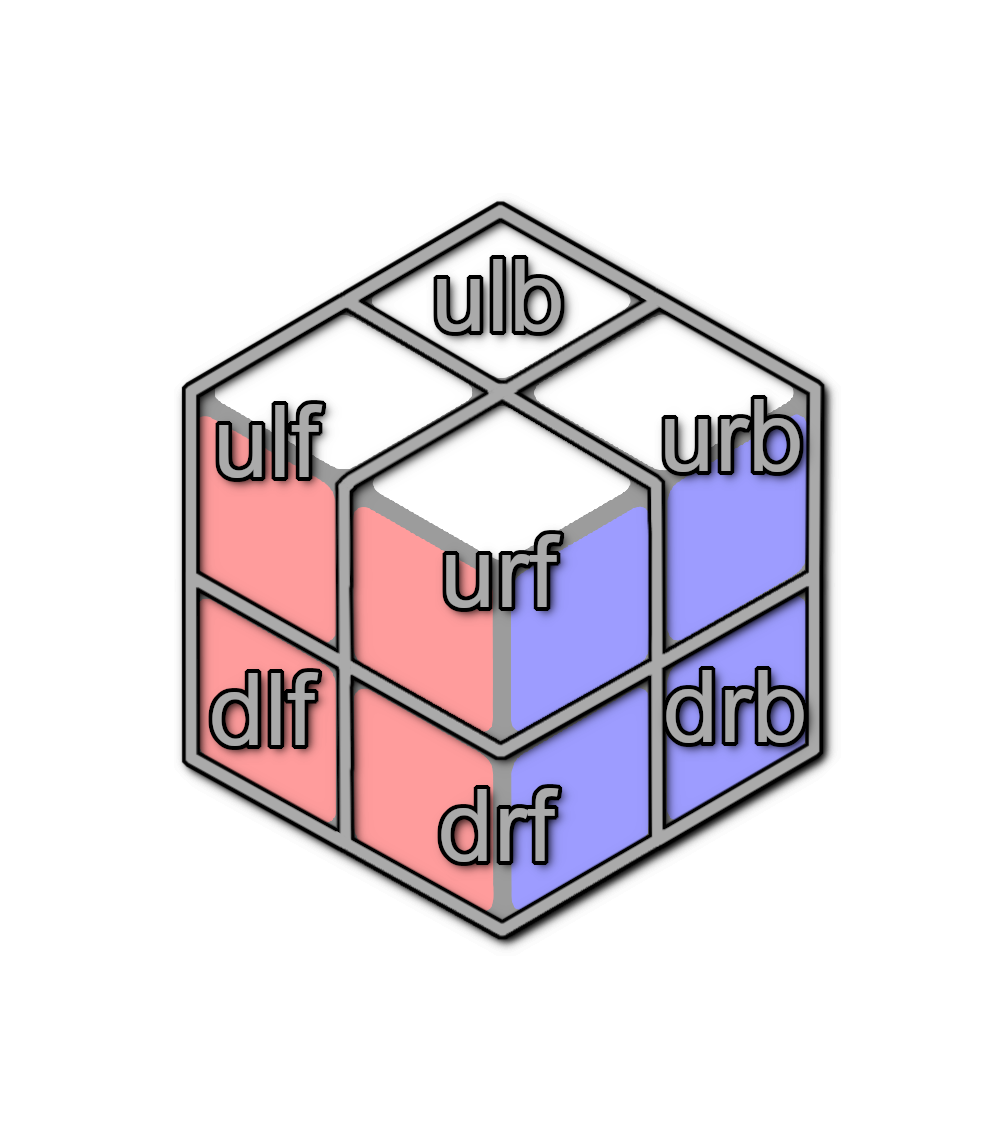
\includegraphics[scale=0.14]{caged_positions.png} \\
\caption[Namen der Steinpositionen im Würfel]{Namen der Steinpositionen im Würfel}
\label{Abbildung_SteinpositionNamen}
\end{figure}

\begin{figure}[h]
\centering
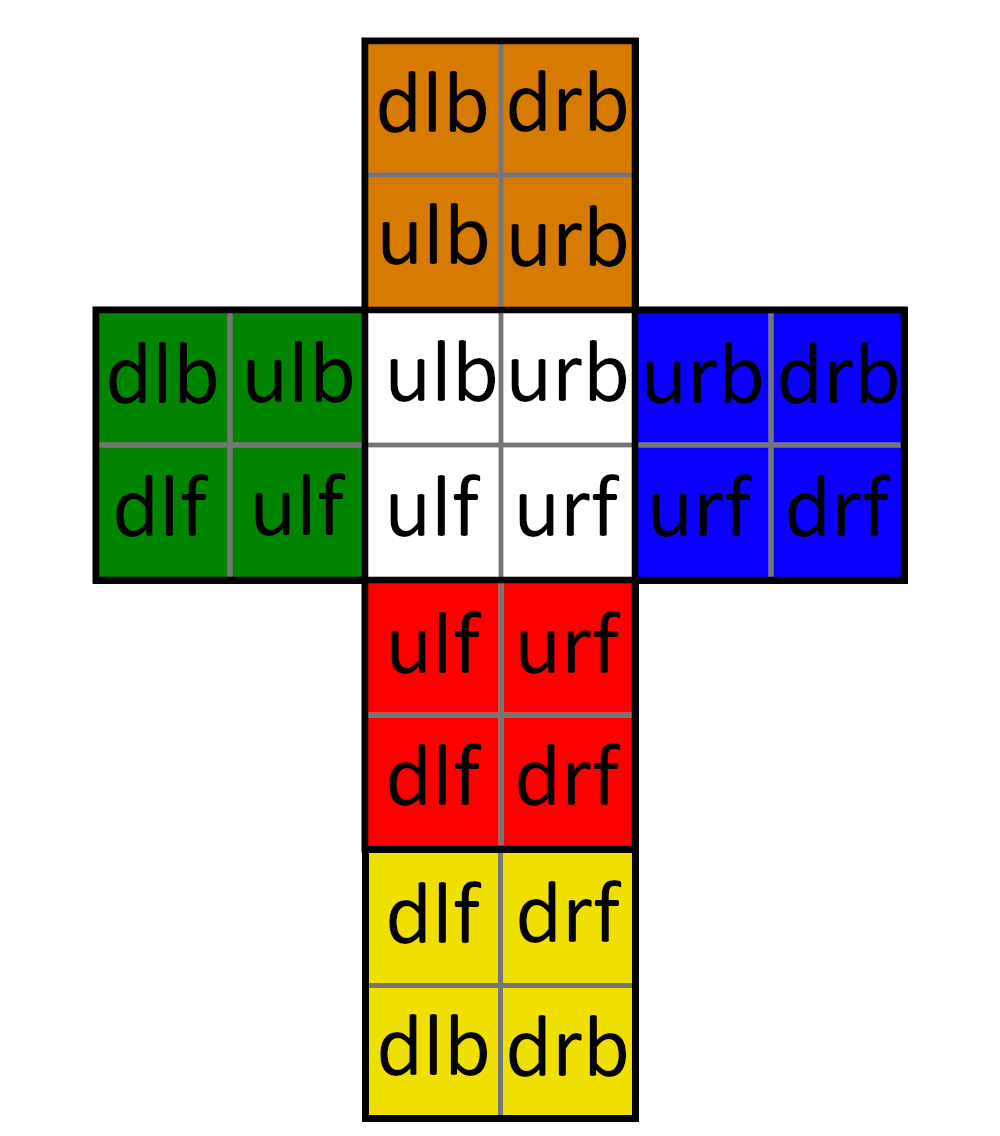
\includegraphics[scale=0.15]{foldedout_cage.png}
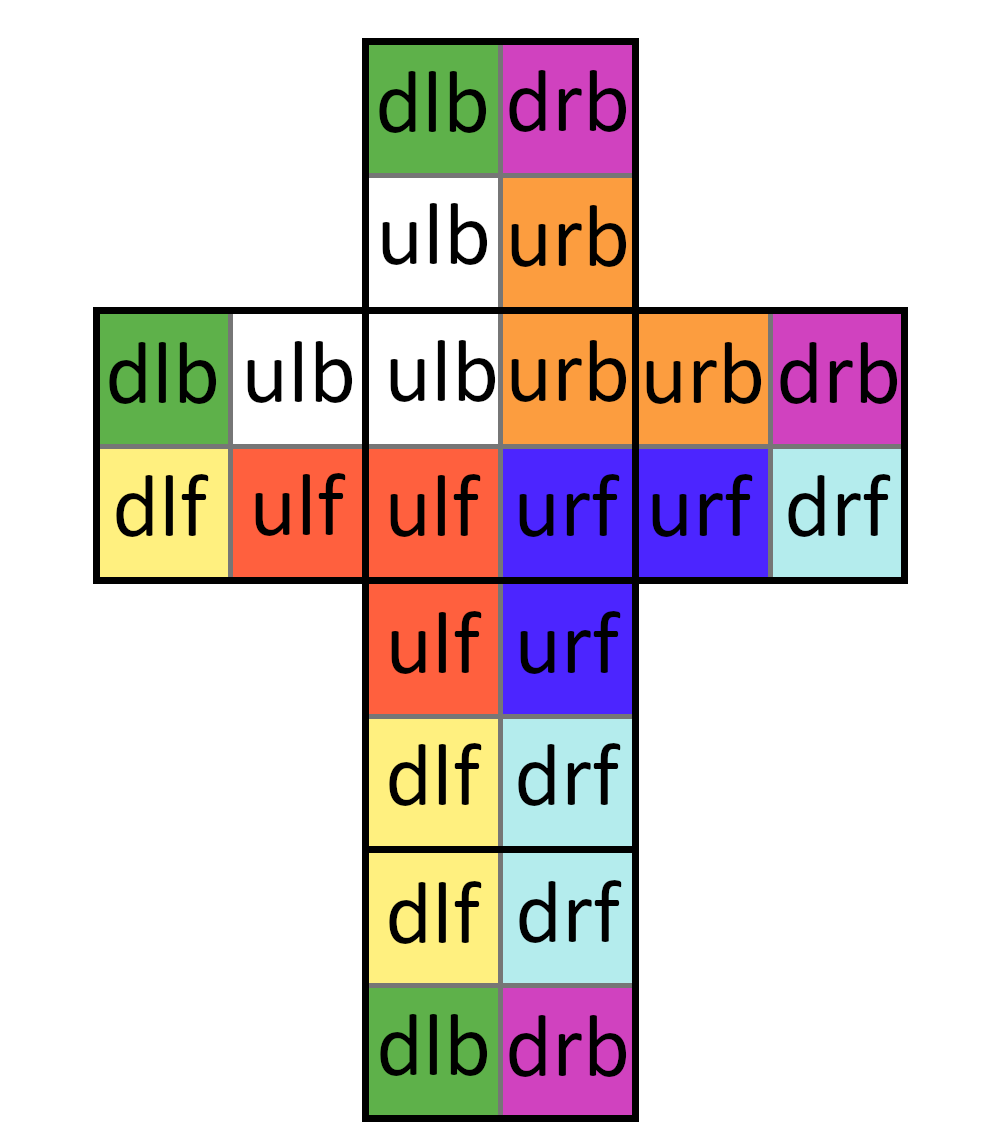
\includegraphics[scale=0.15]{foldedout_cage_color.png}
\caption[Aufgeklappter Würfel mit Namen der Steinpositionen]{Aufgeklappter Würfel mit Namen der Steinpositionen}
\label{Abbildung_SteinpositionNamenFoldetOut}
\end{figure}
Jeder Steinposition wird ein einzigartiger Name zugeordnet, um sich darauf zu beziehen. Dabei wird davon ausgegangen, dass die weiße Seite in der Startkonfiguration oben ist und die rote Seite vorne. Die Steinpositionen werden mit 3 Buchstaben beschrieben, die aus den Kürzeln \textit{u, d, r, l, f, b} bestehen. Diese Kürzel stehen für \textit{up, down, right, left, front, back}. \\
Somit heißt die Steinposition oben links beispielsweise \textit{ulf} (für \textit{up}, \textit{left} und \textit{front}). 
Jeder Stein bekommt zu dem einen eindeutigen Namen, der seiner Steinposition im gelösten Zustand entspricht. Beispielsweise liegt der Stein \textit{ulf} im gelösten Zustand an der Steinposition \textit{ulf}.

Nun wird zur Veranschaulichung die Permutation $\sigma_U$ für eine Drehung der oberen Ebene um 90$^\circ$ im Uhrzeigersinn definiert. Grundlagen zu Permutationen und der Zykelschreibeweise wurden in Abschnitt \ref{Abschnitt_PermutationZykel} erklärt.
Hier wird $\sigma_U$ hergeleitet, ausführlich beschrieben und verschiedene Schreibweisen angegeben. Die Herleitung der weiteren Drehungen funktioniert analog. 
Die Drehung der oberen Ebene ist in Abbildung \ref{Abbildung_SteinpositionnamenNachU} grafisch dargestellt.
\begin{figure}[h]
\centering
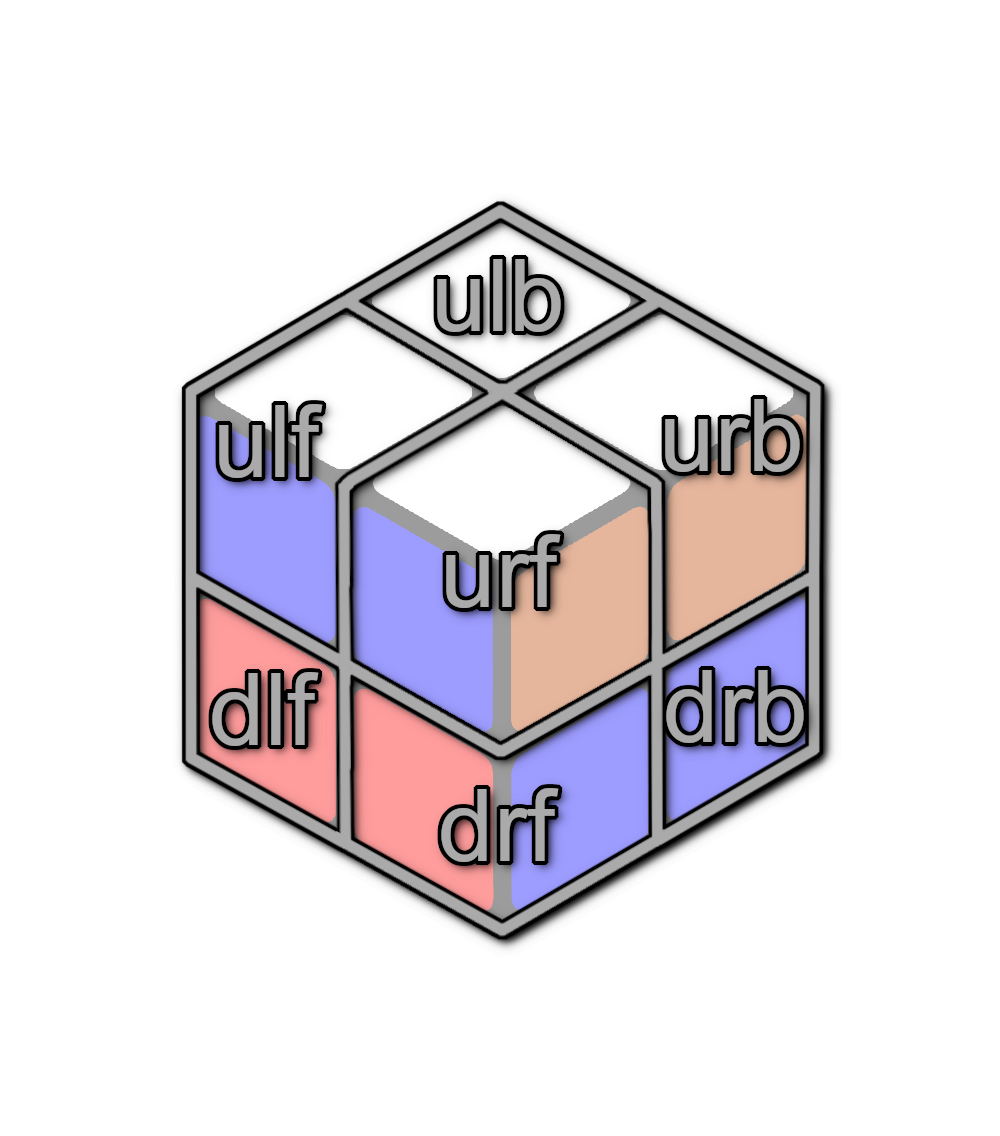
\includegraphics[scale=0.13]{caged_spin.png}
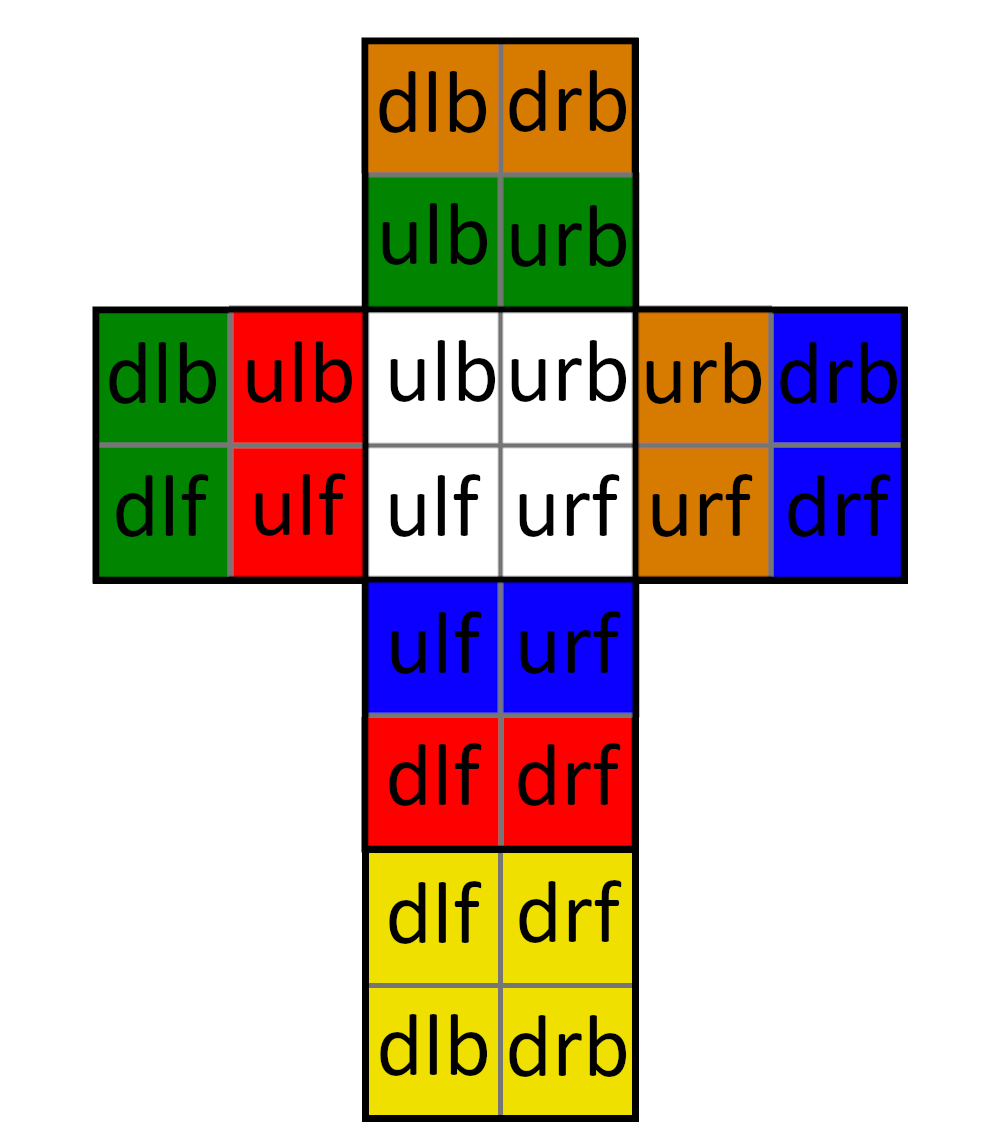
\includegraphics[scale=0.13]{foldedout_spin.png}
\caption[Steinpositionen nach Zug $U$]{Steinpositionen nach Zug $U$}
\label{Abbildung_SteinpositionnamenNachU}
\end{figure}

In Abbildung \ref{Abbildung_SteinpositionnamenNachU} ist zu sehen, dass die Steine der unteren Ebene nicht bewegt wurden. Die Positionen der oberen Ebene haben sich um einen Stein im Uhrzeigersinn verschoben. Daraus ergeben sich folgende Funktionen $\sigma_U$:
\begin{alignat*}{4}
& \sigma_U(\textit{ulf})=\textit{ulb} \ \ \ \ \ \ \ & \sigma_U(\textit{ulb})=\textit{urb} \ \ \ \ \ \ \ & \sigma_U(\textit{urb})=\textit{urf} \ \ \ \ \ \ \ & \sigma_U(\textit{urf})=\textit{ulf} \\
& \sigma_U(\textit{dlf})=\textit{dlf} \ \ \ \ \ \ \ & \sigma_U(\textit{dlb})=\textit{dlb} \ \ \ \ \ \ \ & \sigma_U(\textit{drb})=\textit{drb} \ \ \ \ \ \ \ & \sigma_U(\textit{drf})=\textit{drf} 
\end{alignat*}

Üblich ist auch die Notation der Form $i \mapsto j$: 
\begin{alignat*}{4}
& \textit{ulf} \mapsto \textit{ulb} \ \ \ \ \ \ \ \ & \textit{ulb} \mapsto \textit{urb} \ \ \ \ \ \ \ \ & \textit{urb} \mapsto \textit{urf} \ \ \ \ \ \ \ \ & \textit{urf} \mapsto \textit{ulf} \\
& \textit{dlf} \mapsto \textit{dlf} \ \ \ \ \ \ \ \ & \textit{dlb} \mapsto \textit{dlb} \ \ \ \ \ \ \ \ \ & \textit{drb} \mapsto \textit{drb} \ \ \ \ \ \ \ \ & \textit{drf} \mapsto \textit{drf} 
\end{alignat*}

Daraus entstehen folgende Zykel: $\sigma_U = \ ( \textit{ulf} \ \textit{ulb} \ \textit{urb} \ \textit{urf} )\ ( \textit{dlf} )\ ( \textit{dlb} )\ ( \textit{drb} )\ ( \textit{drf} )$

Einelementige Zykel müssen nicht aufgeschrieben werden. Dann ergibt sich $\sigma_U = \ ( \textit{ulf} \ \textit{ulb} \ \textit{urb} \ \textit{urf} )$, was den Zykel beschreibt, in dem die Steine rotiert werden, wenn die obere Ebene gedreht wird. 


Die Drehungen aller Ebenen können durch folgende Zykel beschrieben werden: 
\begin{align*}
\sigma_U & =\ ( \textit{ulf} \ \textit{ulb} \ \textit{urb} \ \textit{urf} ) \\
\sigma_D & =\ ( \textit{dlf} \ \textit{drf} \ \textit{drb} \ \textit{dlb} ) \\
\sigma_F & =\ ( \textit{ulf} \ \textit{urf} \ \textit{drf} \ \textit{dlf} ) \\
\sigma_B & =\ ( \textit{ulb} \ \textit{dlb} \ \textit{drb} \ \textit{urb} ) \\
\sigma_L & =\ ( \textit{ulb} \ \textit{ulf} \ \textit{dlf} \ \textit{dlb} ) \\
\sigma_R & =\ ( \textit{urb} \ \textit{drb} \ \textit{drf} \ \textit{urf} ) 
\end{align*}

Die Indizes an den Funktionen $\sigma$ stehen für die verschiedenen Grundzüge des Würfels. Diese wurden in Abschnitt \ref{Abschnitt_GrundzügeWürfel} erklärt.

Die Identitätspermutation wird als $\sigma=1$ geschrieben. Somit wird der leere Zug folgendermaßen definiert:
\begin{align*}
\sigma_N = 1
\end{align*}

%
%
%
%
%
%
%
%
%
%
%=======================================================================================================
%
%
%
%
%
%
%
%
%
%
\subsection{Ausrichtung der Steine} 
 \label{Abschnitt_AusrichtungDerSteine}
Der \Ttwo Würfel besteht aus 8 Ecksteinen, die jeweils 3 Farbflächen haben. Somit hat jeder Stein 3 mögliche Ausrichtungen. 
Um die Ausrichtung der Steine zu erkennen, bekommen die Würfelpositionen an einer Farbfläche eine Nummer zugeordnet. Dafür werden die weißen und die gelben Seiten markiert und nummeriert. Auf diese Nummern wird sich als $x_i$ mit $i \in \lbrace 1, 2, 3, 4, 5, 6, 7, 8 \rbrace$ bezogen - mit $x_1$ als Position 1, $x_2$ als Position 2, usw.

Außerdem bekommt jeder Stein an jeder Farbfläche eine Zahlenzuordnung. Da jeder Stein 3 Ausrichtungen haben kann, werden die Farbflächen mit 0, 1 und 2 nummeriert. Die Nummerierung beginnt mit der weißen bzw. gelben Fläche bei 0 und zählt dann im Uhrzeigersinn die Flächen. 
In der Startkonfiguration sind alle $x_i = 0$, der Vektor $x$ ist dann $(0, 0, 0, 0, 0, 0, 0, 0)$. Das wird kurz als $x=0$ geschrieben.

\begin{figure}[H]
\centering
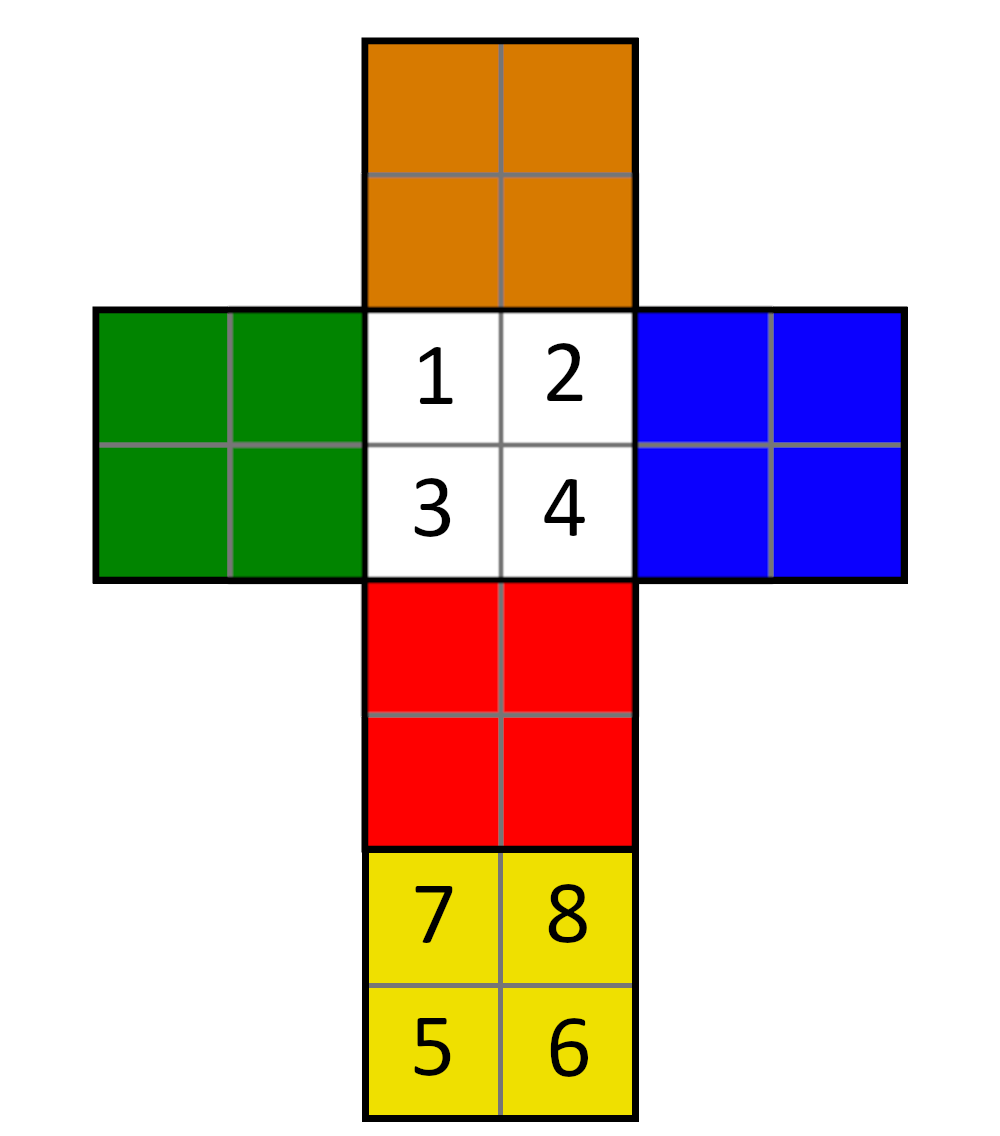
\includegraphics[scale=0.13]{foldedout_numbers.png}
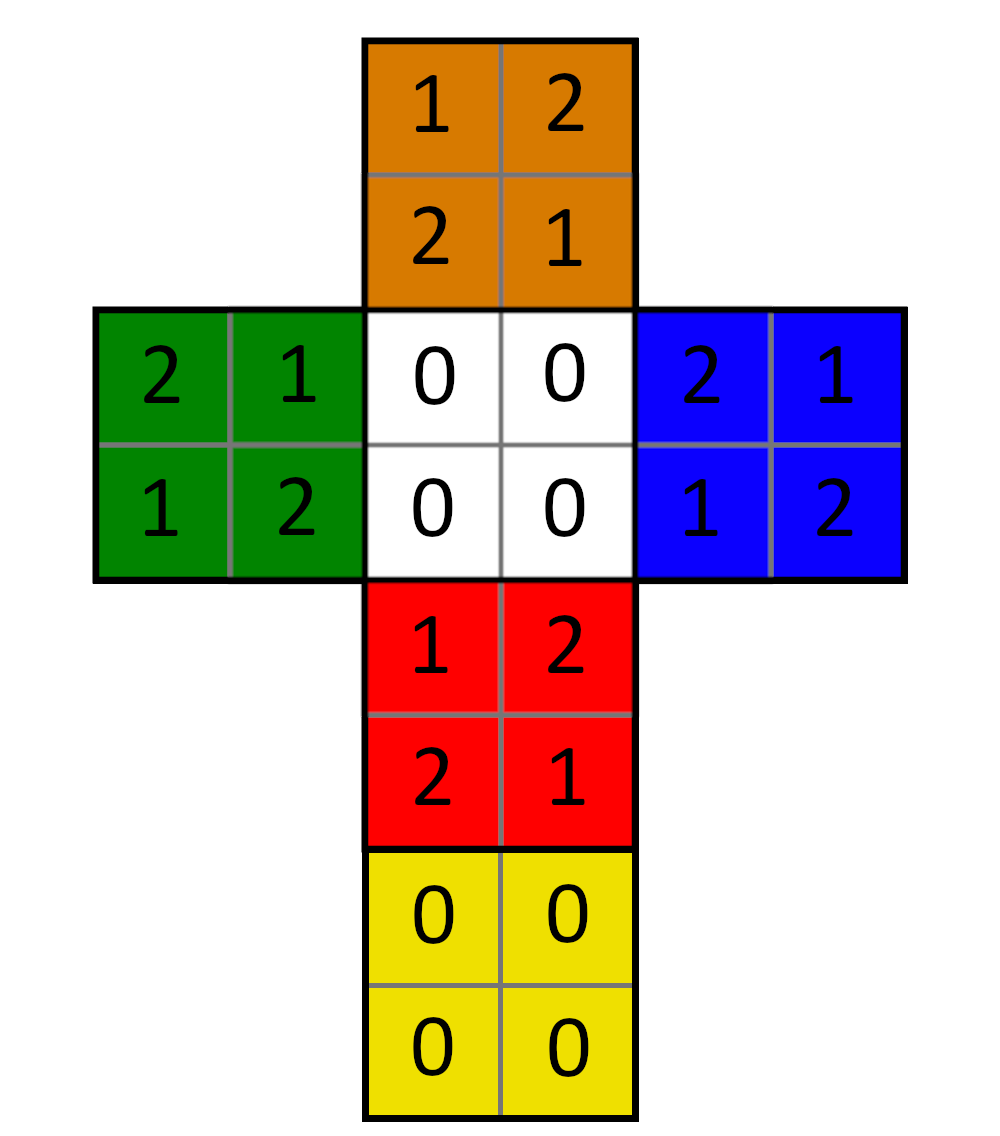
\includegraphics[scale=0.13]{foldedout_012.png}
\caption[Markierungen $x_i$ (links), Farbflächennummern (rechts)]{Ausgeklappter Würfel mit Markierungen für $x_i$ (links) und Farbflächennummerierungen (rechts) }
\end{figure}


Im Folgenden wird der Zug $R$ ausgeführt (s. Abbildung \ref{Abbildung_XnachZugR}) und die Veränderung der Farbflächennummerierung zur Veranschaulichung dargestellt. $R$ ist eine Drehung der rechten Ebene um 90$^\circ$ im Uhrzeigersinn. 
Die Kennzeichnungen $x_{1-8}$ bleiben an der gleichen Position. Die Nummerierungen  der Farbflächen ändern sich mit Drehung der Ebene und ermöglichen so eine Zuordnung der Ecksteinausrichtung. 
Die linke Seite des Würfels wird dabei nicht beeinflusst. Deshalb sind die Flächen an den Positionen $x_1, x_3, x_5, x_7$ alle 0, da sie der der linken Hälfte des Würfels zugeordnet sind.
Die anderen Positionen von $x$ zeigen nun aber andere Farbflächen: 
\begin{align*}
x_2 = 2 \ \ \ \ \ \ x_4 = 1 \ \ \ \ \ \ x_6 = 1 \ \ \ \ \ \ x_8 = 2  
\end{align*}
Daher gilt $x = (0, 2, 0, 1, 0, 1, 0, 2)$ nach dem Zug $R$. Das ist auch anhand von Abbildung \ref{Abbildung_XnachZugR} zu erkennen. Links sind dort die Positionen der Vektoreinträge von $x$ abgebildet und rechts sieht man den Würfel mit den Farbflächennummerierungen, nachdem der Zug $R$ ausgeführt wurde.
\begin{figure}[H]
\centering
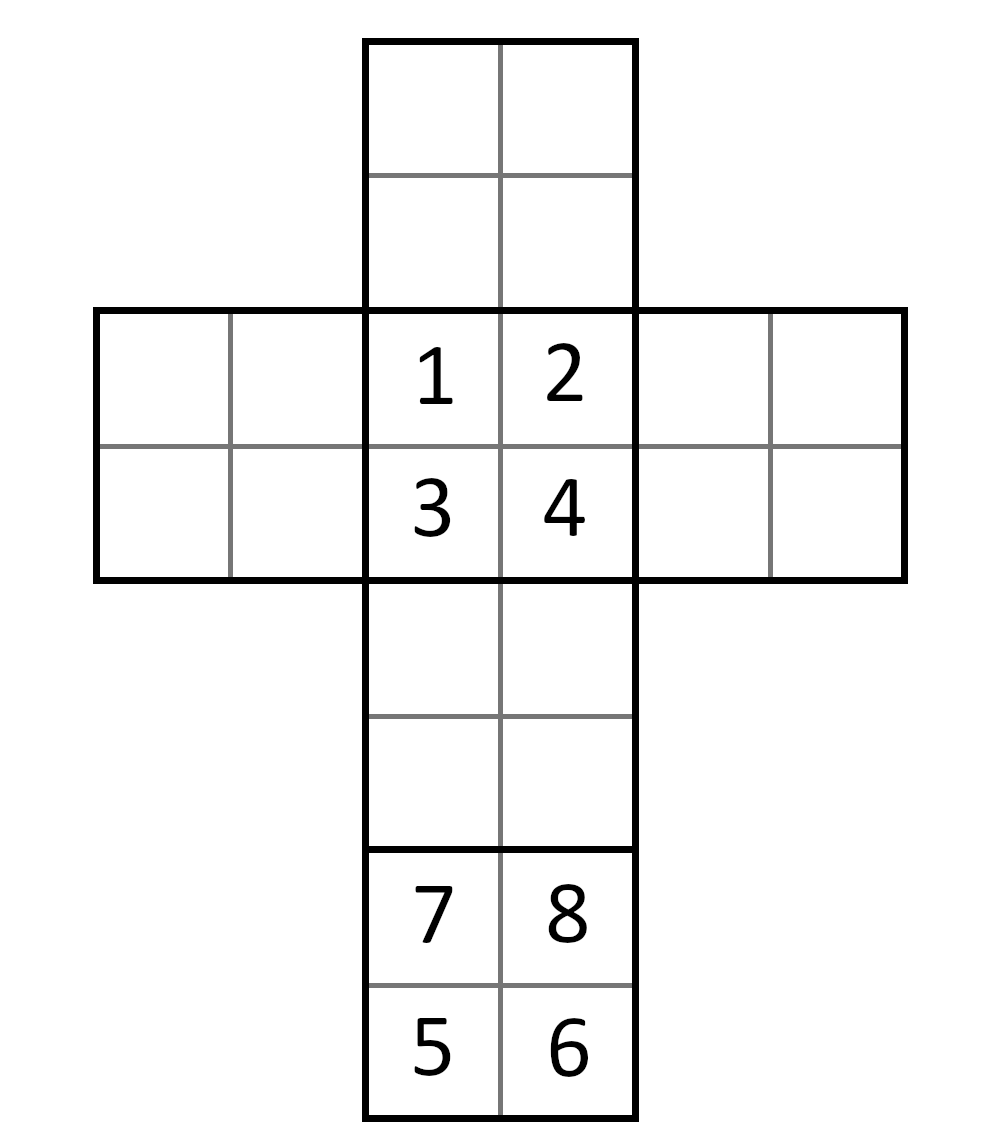
\includegraphics[scale=0.13]{foldedout_012_white.png}
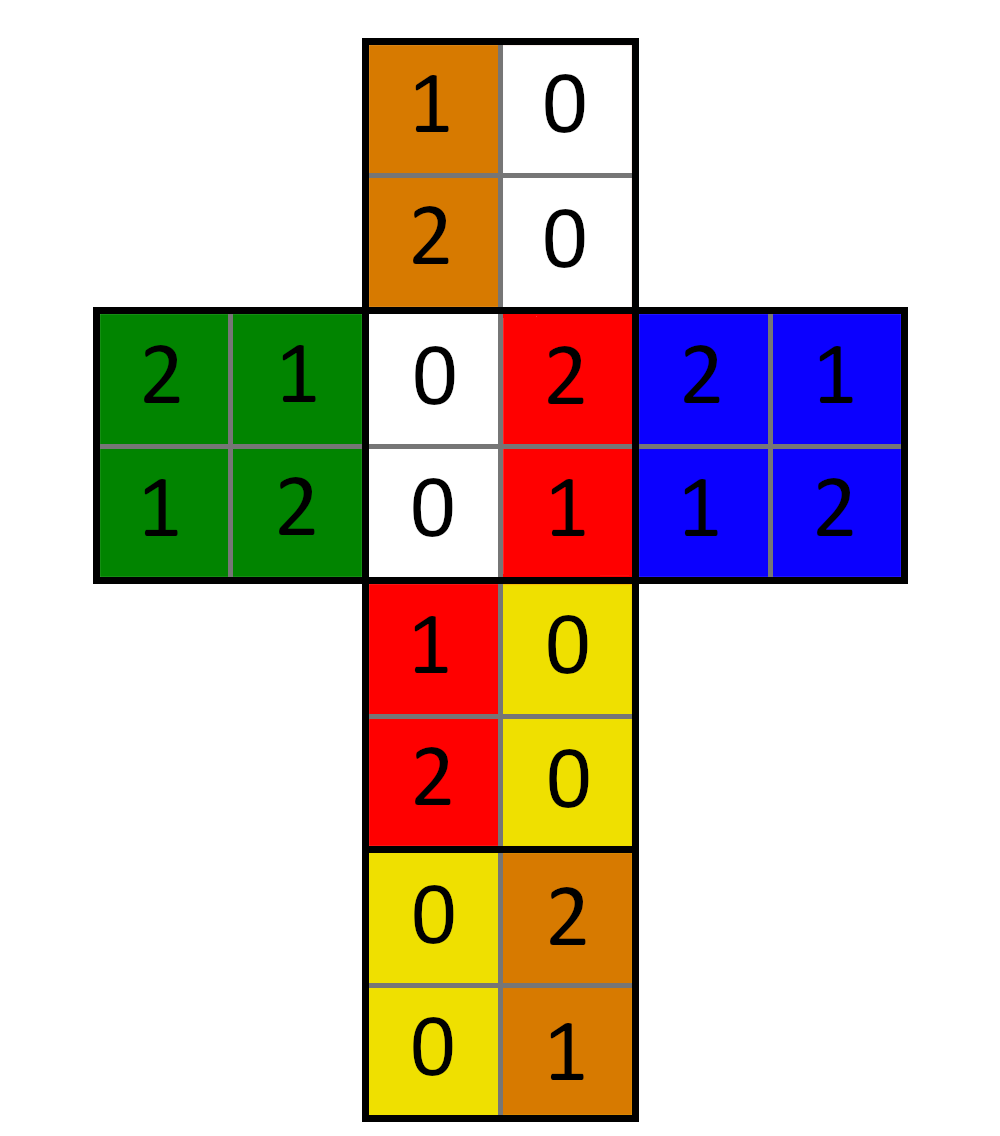
\includegraphics[scale=0.13]{foldedout_012_spin.png}
\caption[Links: $x_1$ bis $x_8$, rechts: Veränderung nach dem Zug $R$]{Links: Positionen $x_1$ bis $x_8$, rechts: Veränderung der nummerierten Ecksteine nach dem Zug $R$}
\label{Abbildung_XnachZugR}
\end{figure}

Anhand des Beispielzuges $R$ kann für jeden Vektoreintrag eine Funktion $\Gamma_R$ aufgestellt werden, die die Veränderung des Vektors $x$ nach Ausführen des Zuges $R$ bei jeder beliebigen Ausgangskonfiguration beschreibt. Da $x_1, x_3, x_5$ und $x_7$ nicht beeinflusst werden, bleiben diese unverändert. Der Vektoreintrag, der durch $\Gamma_R$ in den Folgewert verändert wird, ist im Folgenden schwarz hervorgehoben. Alle anderen Einträge sind ausgegraut.
\begin{align*}
& \Gamma_{R_1}(\textcolor{gray}{(\textcolor{black}{x_1}, x_2, x_3, x_4, x_5, x_6, x_7, x_8  )})=\textcolor{gray}{(\textcolor{black}{x_1}, x_2, x_3, x_4, x_5, x_6, x_7, x_8  )} \\
& \Gamma_{R_3}(\textcolor{gray}{(x_1, x_2, \textcolor{black}{x_3}, x_4, x_5, x_6, x_7, x_8  )})=\textcolor{gray}{(x_1, x_2, \textcolor{black}{x_3}, x_4, x_5, x_6, x_7, x_8  )} \\
& \Gamma_{R_5}(\textcolor{gray}{(x_1, x_2, x_3, x_4, \textcolor{black}{x_5}, x_6, x_7, x_8  )})=\textcolor{gray}{(x_1, x_2, x_3, x_4, \textcolor{black}{x_5}, x_6, x_7, x_8  )}\\
& \Gamma_{R_7}(\textcolor{gray}{(x_1, x_2, x_3, x_4, x_5, x_6,\textcolor{black}{x_7}, x_8  )})=\textcolor{gray}{(x_1, x_2, x_3, x_4, x_5, x_6, \textcolor{black}{x_7}, x_8  )} 
\end{align*}
Die Flächen an den Positionen $x_2, x_4, x_6$ und $x_8$ werden in Abhängigkeit der vorherigen Steinausrichtungen verändert. Es ergeben sich folgende Funktionen für die Positionen $x_2, x_4, x_6$ und $x_8$ nach dem Zug $R$: 


\begin{align*}
\Gamma_{R_2}(\textcolor{gray}{(x_1, \textcolor{black}{x_2}, x_3, x_4, x_5, x_6, x_7, x_8  )})= \begin{cases}
\textcolor{gray}{(x_1, \textcolor{black}{2}, x_3, x_4, x_5, x_6, x_7, x_8  )} & \ \text{falls } x_4 = 0 \\ 
\textcolor{gray}{(x_1, \textcolor{black}{0}, x_3, x_4, x_5, x_6, x_7, x_8  )} & \ \text{falls } x_4 = 1 \\
\textcolor{gray}{(x_1, \textcolor{black}{1}, x_3, x_4, x_5, x_6, x_7, x_8  )} & \ \text{falls } x_4 = 2 
\end{cases}
\end{align*}

Die Funktion $\Gamma_{R_2}$ verändert den Vektoreintrag $x_2$ nach Ausführen des Zuges $R$ in Abhängigkeit des Vektoreintrages $x_4$. Die Farbfläche, die durch das Ausführen des Zuges auf die Position $x_2$ gelangt, steht in direkter Abhängigkeit der Farbfläche an Position $x_4$, da es sich dabei um denselben Stein handelt. Wenn sich an der Position $x_4$ zu Beginn eine Farbfläche mit dem Wert 0 befindet, so wird die Farbfläche mit dem Wert 2 desselben Steines durch Ausführen von $R$ an die Position $x_2$ gebracht. Das ist auch in Abbildung \ref{Abbildung_UebergangsfunktionR} zu sehen. Analog funktioniert das mit $x_4 = 1$ (dann wird $x_2 = 0$) und $x_4=2$ (dann wird $x_2 = 1$). 

\begin{figure}[H]
\centering
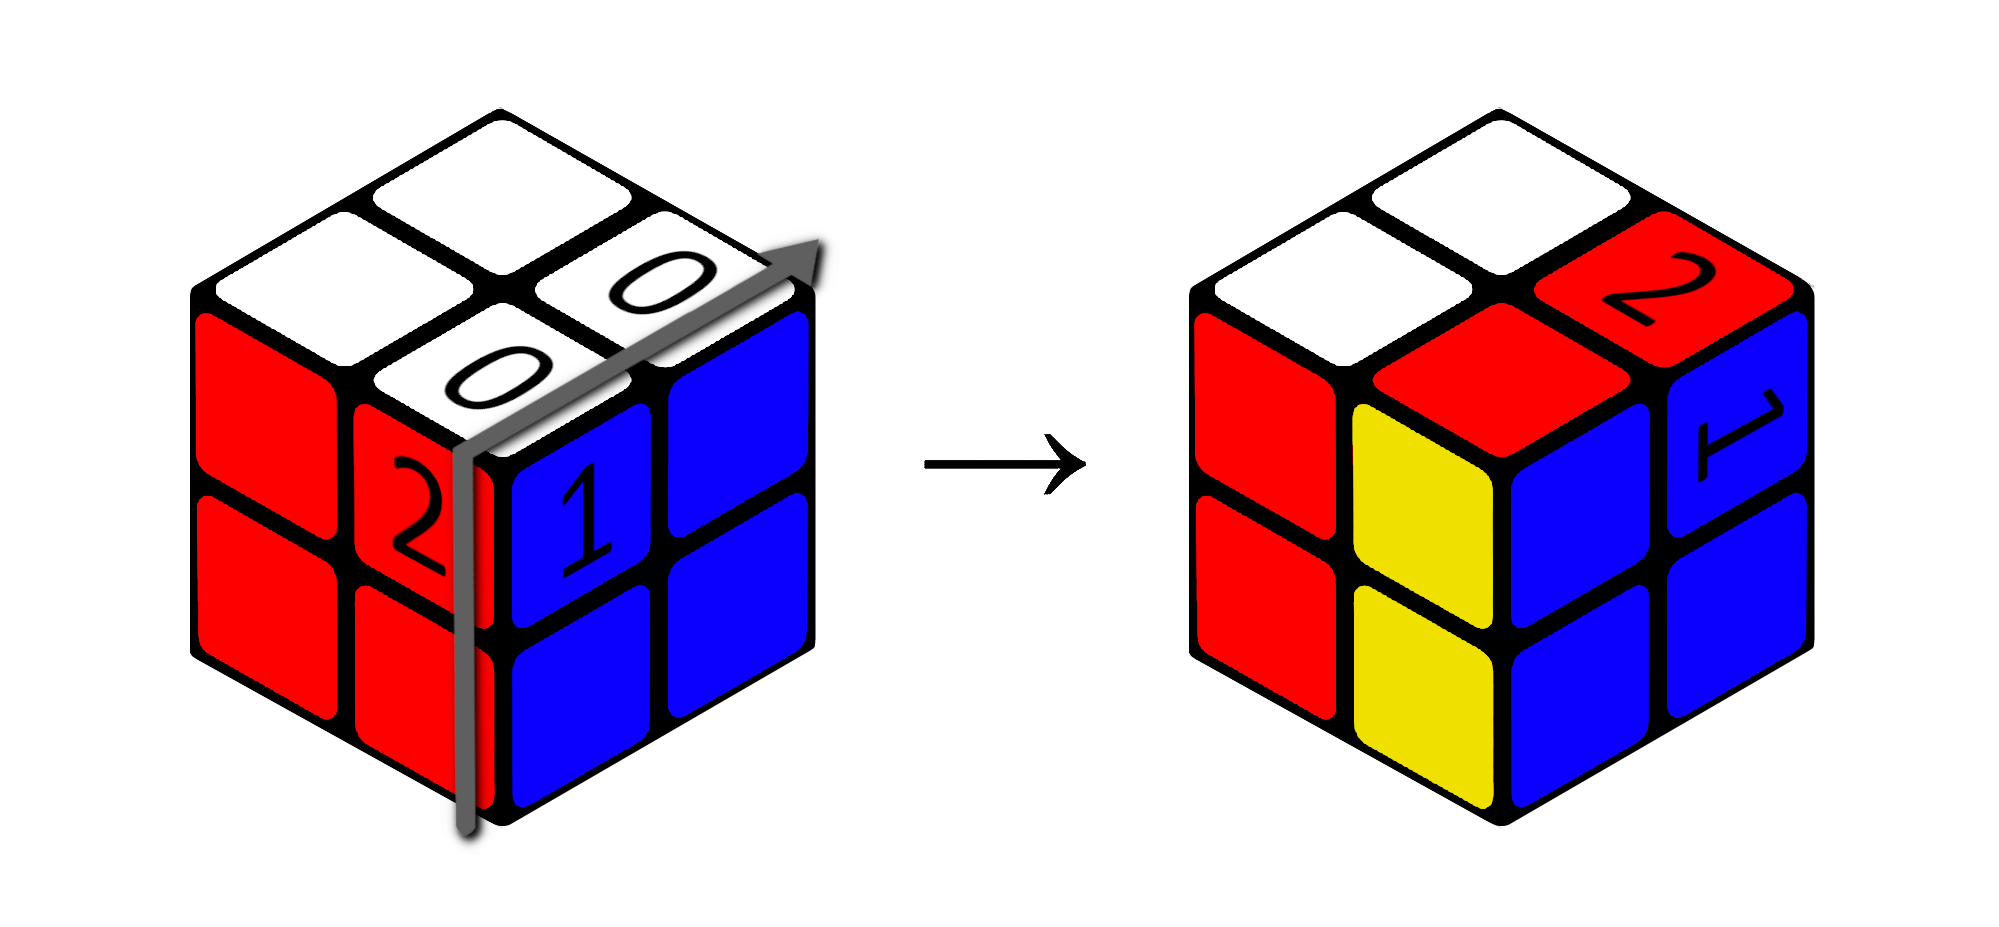
\includegraphics[scale=0.13]{UebergangsfunktionR.png}
\caption{Veränderung von Vektoreintrag $x_2$ bei Zug $R$}
\label{Abbildung_UebergangsfunktionR}
\end{figure}

Die anderen Funktionen für die Veränderung des Vektors $x$ werden ebenfalls durch die Abhängigkeit der Steinflächen zueinander definiert.

\begin{align*}
\Gamma_{R_4}(\textcolor{gray}{(x_1, x_2, x_3, \textcolor{black}{x_4}, x_5, x_6, x_7, x_8  )})= \begin{cases}
\textcolor{gray}{(x_1, x_2, x_3, \textcolor{black}{1}, x_5, x_6, x_7, x_8  )} & \ \text{falls } x_8 = 0 \\ 
\textcolor{gray}{(x_1, x_2, x_3, \textcolor{black}{2}, x_5, x_6, x_7, x_8  )} & \ \text{falls } x_8 = 1 \\
\textcolor{gray}{(x_1, x_2, x_3, \textcolor{black}{0}, x_5, x_6, x_7, x_8  )} & \ \text{falls } x_8 = 2 
\end{cases} \\
\\
\Gamma_{R_6}(\textcolor{gray}{(x_1, x_2, x_3, x_4, x_5, \textcolor{black}{x_6}, x_7, x_8  )})= \begin{cases}
\textcolor{gray}{(x_1, x_2, x_3, x_4, x_5, \textcolor{black}{1}, x_7, x_8  )} & \ \text{falls } x_2 = 0 \\ 
\textcolor{gray}{(x_1, x_2, x_3, x_4, x_5, \textcolor{black}{2}, x_7, x_8  )} & \ \text{falls } x_2 = 1 \\
\textcolor{gray}{(x_1, x_2, x_3, x_4, x_5, \textcolor{black}{0}, x_7, x_8  )} & \ \text{falls } x_2 = 2 
\end{cases} \\
\\
\Gamma_{R_8}(\textcolor{gray}{(x_1, x_2, x_3, x_4, x_5, x_6, x_7, \textcolor{black}{x_8})})= \begin{cases}
\textcolor{gray}{(x_1, x_2, x_3, x_4, x_5, x_6, x_7, \textcolor{black}{2})} & \ \text{falls } x_6 = 0 \\ 
\textcolor{gray}{(x_1, x_2, x_3, x_4, x_5, x_6, x_7, \textcolor{black}{0})} & \ \text{falls } x_6 = 1 \\
\textcolor{gray}{(x_1, x_2, x_3, x_4, x_5, x_6, x_7, \textcolor{black}{1})} & \ \text{falls } x_6 = 2 
\end{cases}
\end{align*}







Es gibt für den Zug $R$ acht Funktionen $\Gamma_R$ -- eine für jeden Vektoreintrag. Die Funktionen $\Gamma_{R_2}$ und $\Gamma_{R_8}$ verändern verschiedene Vektoreinträge auf die gleiche Weise, die Funktionen $\Gamma_{R_4}$ und $\Gamma_{R_6}$ ebenfalls. Auch die Funktionen $\Gamma_{R_1}, \Gamma_{R_3}, \Gamma_{R_5}$ und $\Gamma_{R_7}$ arbeiten analog. Da diese Funktionen in Hinblick auf Ein- und Aufgabe gleich aufgebaut sind, reichen drei verschiedene Funktionen für die Veränderung jedes Vektoreintrags aus $x$ nach dem Zug $R$ aus.
\\

\begin{minipage}{0.35\textwidth}
\centering
$g(x)= \begin{cases}
2 & \ \text{falls } x = 0 \\ 
0 & \ \text{falls } x = 1 \\
1 & \ \text{falls } x = 2 
\end{cases}$
\end{minipage}
\begin{minipage}{0.35\textwidth}
\centering
$h(x)= \begin{cases}
1 & \ \text{falls } x = 0 \\ 
2 & \ \text{falls } x = 1 \\
0 & \ \text{falls } x = 2 
\end{cases}$
\end{minipage}
\begin{minipage}{0.3\textwidth}
\centering
$i(x) = x$
\end{minipage}
\vspace*{1em}

Die Funktionen $g$ und $h$ können auch ohne Fallunterscheidung mit modulo 3 geschrieben werden:
\begin{align*}
g(x)=(x+2) \hspace*{-0.5em} \mod 3 \ \ \ \ \ \ \ \ h(x) = (x+1) \hspace*{-0.5em} \mod 3
\end{align*}

Da \textit{i} die Identitätsfunktion ist, kann diese weggelassen werden.
Mit den Funktionen \textit{g} und \textit{h} lassen sich die Ausrichtungen der Steine nach dem Zug $R$ bestimmen. So wird der Vektor $x$ nach dem Zug $R$ durch die Funktion $\gamma_R$ verändert, die sich aus den Funktionen $\Gamma_{R_{1-8}}$ zusammensetzt:
\begin{align*}
& \gamma_R \left( (x_1, x_2, x_3, x_4, x_5, x_6, x_7, x_8  ) \right) \\ 
& =  \left( x_1, g(x_4), x_3, h(x_8), x_5, h(x_2), x_7, g(x_6) \right)
\end{align*}

Analog dazu gibt es für jeden der sechs Grundzüge eine Funktion $\gamma$, die die Veränderung der Steinausrichtung realisiert. Diese Funktionen lassen sich ebenfalls mit den Funktionen $g$, $h$ und $i$ bilden.
\begin{align*}
& \gamma_U \left( (x_1, x_2, x_3, x_4, x_5, x_6, x_7, x_8  ) \right) \\ 
& =  \left( x_3, x_1, x_4, x_2, x_5, x_6, x_7, x_8 \right) \\
\\ 
& \gamma_D \left( (x_1, x_2, x_3, x_4, x_5, x_6, x_7, x_8  ) \right) \\ 
& =  \left( x_1, x_2, x_3, x_4, x_6, x_8, x_5, x_7 \right) \\
\\
& \gamma_R \left( (x_1, x_2, x_3, x_4, x_5, x_6, x_7, x_8  ) \right) \\ 
& =  \left( x_1, g(x_4), x_3, h(x_8), x_5, h(x_2), x_7, g(x_6) \right) \\ 
\\
& \gamma_L \left( (x_1, x_2, x_3, x_4, x_5, x_6, x_7, x_8  ) \right) \\ 
& =   (h(x_5), x_2, g(x_1), x_4, g(x_7), x_6, h(x_3), x_8) \\ 
\\
& \gamma_F \left( (x_1, x_2, x_3, x_4, x_5, x_6, x_7, x_8  ) \right) \\ 
& =  \left( x_1, x_2, h(x_7), g(x_3), x_5, x_6, g(x_8), h(x_4) \right) \\
\\
& \gamma_B \left( (x_1, x_2, x_3, x_4, x_5, x_6, x_7, x_8  ) \right) \\ 
& =  \left( g(x_2), h(x_6), x_3, x_4, h(x_1), g(x_5), x_7, x_8 \right)
\end{align*}
Bei dem leeren Zug bleibt der Vektor undverändert. Die folgende Funktion ergibt sich:
\begin{align*}
& \gamma_N \left( (x_1, x_2, x_3, x_4, x_5, x_6, x_7, x_8  ) \right) \ \ \ \ \ \ \ \ \ \ \ \ \ \ \ \\ 
& =  \left( x_1, x_2, x_3, x_4, x_5, x_6, x_7, x_8 \right)
\end{align*}

Das oben genannte Beispiel des Zuges $R$ (s. Abbildung \ref{Abbildung_XnachZugR}) wird nun schrittweise mithilfe von $\gamma_R$ berechnet. Dafür befindet sich der Würfel zu Beginn in der Startkonfiguration ($x = (0, 0, 0, 0, 0, 0, 0, 0)$). Die Steinposition wird hier nicht berücksichtigt. Wenn der Zug $R$ ausgeführt wird, wird $\gamma_R( (0, 0, 0, 0, 0, 0, 0, 0) )$ berechnet:
\begin{align*}
& \gamma_R( (0, 0, 0, 0, 0, 0, 0, 0) ) \\
& = (0, g(0), 0, h(0), 0, h(0), 0, g(0)) \\
& = (0, 2, 0, 1, 0, 1, 0, 2)
\end{align*}

Der Vektor $x$ lautet nach dem Zug $R$ von der Startkonfiguration ausgehend: $(0, 2, 0, 1, 0, 1, 0, 2)$. 

%
%
%
%
%=======================================================================================================
%
%
%
%
%
%
\subsection{Züge ausführen}

\label{Abschnitt_ZuegeAusfuehren}

Eine Würfelkonfiguration $C=(\sigma, x)$ wird durch das Ausführen eines Zuges verändert.
Die Permutation $\sigma$ repräsentiert dann die neue Position der Steine im Würfel und der Vektor $x$ die Ausrichtung der Steine. Ein Zug $Z$ kann dabei einer der Grundzüge ($U,D,R,L,F,B$) oder eine Aneinanderreihung von Grundzügen sein. Die Grundzüge wurden in Kapitel \ref{Abschnitt_GrundzügeWürfel} beschrieben.

Wird ein Zug $Z$ auf einer Würfelkonfiguration $C$ ausgeführt, wird das als $C \cdot Z$ geschrieben. Das Ergebnis von $C \cdot Z$ ist dann eine neue Folgekonfiguration $C'$.

Im Folgenden wird der Zug $(LLFF)^3$ beispielhaft auf die Startkonfiguration angewandt. Die Startkonfiguration ist $C=(1,0)$. Sie wird durch das dreifache Ausführen des Zuges $LLFF$ ($LLFF^3 = LLFFLLFFLLFF$) schrittweise verändert.
Die Position der Steine -- dargestellt durch $\sigma$ -- verändert sich nach dem ersten Ausführen von $LLFF$ folgendermaßen:

\begin{center}
\begin{tabular}{ccccccccc}
\toprule
\textbf{Zug} & \textbf{ulb} & \textbf{urb} & \textbf{ulf} & \textbf{urf} & \textbf{dlb} & \textbf{drb} & \textbf{dlf} & \textbf{drf} \\
\midrule

L & ulf & \textcolor{gray}{urb} & dlf & \textcolor{gray}{urf} & ulb & \textcolor{gray}{drb} & dlb & \textcolor{gray}{drf} \\

L & dlf & \textcolor{gray}{urb} & dlb & \textcolor{gray}{urf} & ulf & \textcolor{gray}{drb} & ulb & \textcolor{gray}{drf} \\

F & ulf & \textcolor{gray}{urb} & \textcolor{gray}{dlb} & drf & urf & \textcolor{gray}{drb} & \textcolor{gray}{ulb} & dlf \\

F & urf & \textcolor{gray}{urb} & \textcolor{gray}{dlb} & dlf & drf & \textcolor{gray}{drb} & \textcolor{gray}{ulb} & ulf \\
\bottomrule
\end{tabular}
\end{center}

Der neue Vektor $x$ wird nach dem Teilzug $LLFF$ durch $\gamma_F(\gamma_F(\gamma_L(\gamma_L(x))))$ berechnet. 
\begin{align*}
 \gamma_F(\gamma_F(\gamma_L(\gamma_L(x)))) \Rightarrow \ & \gamma_F(\gamma_F(\gamma_L(\gamma_L((0,0,0,0,0,0,0,0))))) \\
= \ & \gamma_F(\gamma_F(\gamma_L((h(0),0,g(0),0,g(0),0,h(0),0)))) \\
= \ & \gamma_F(\gamma_F(\gamma_L((1,0,2,0,2,0,1,0)))) \\
= \ & \gamma_F(\gamma_F((h(1),0,g(2),0,g(2),0,h(1),0))) \\
= \ & \gamma_F(\gamma_F((0,0,0,0,0,0,0,0))) \\
= \ & \gamma_F((0,0,h(0),g(0),0,0,g(0),h(0))) \\
= \ & \gamma_F((0,0,1,2,0,0,2,1)) \\
= \ & (0,0,h(1),g(2),0,0,g(2),h(1)) \\
= \ & (0,0,0,0,0,0,0,0)
\end{align*}

Aus dieser Rechnung geht hervor, dass der Vektor nach Ausführen der Drehung $L$ zu $(1,0,2,0,2,0,1,0)$ wird. Wird $L$ dann nochmal ausgeführt, so ist der Vektor wieder $(0,0,0,0,0,0,0,0)$. Der Würfel ist dann aber nicht gelöst, da die Position der Steine ($\sigma$) verändert ist.
Wird nun die Drehung $F$ zweimal ausgeführt, geht der Vektor über $(0,0,1,2,0,0,2,1)$ wieder in  $(0,0,0,0,0,0,0,0)$ über. 

Die Konfiguration $C'$ nach dem ersten Ausführen des Teilzuges $LLFF$ ist somit 
\begin{align*}
C' = ((\textit{ulb} \ \textit{urf} \ \textit{dlf} )\ ( \textit{dlb} \ \textit{drf} \ \textit{ulf} ),(0,0,0,0,0,0,0,0))
\end{align*} 
oder kurz $C' = ((\textit{ulb} \ \textit{urf} \ \textit{dlf} ) \ (\textit{dlb} \ \textit{drf} \ \textit{ulf} ),0)$.

Wenn der Zug $LLFF$ nun erneut ausgeführt wird, verändert der Vektor $x$ sich wieder auf die gleiche Weise und wird wieder $(0,0,0,0,0,0,0,0)$. Die Permutation $\sigma$ der Position ergibt nach dem zweiten Ausführen von $LLFF$: $( \textit{urf} \ \textit{dlf} \ \textit{ulb} ) \ ( \textit{drf} \ \textit{ulf} \ \textit{dlb} )$. Die Folgekonfiguration nach dem zweiten Ausführen von $LLFF$ ist somit Folgende:
\begin{align*}
C'' = (( \textit{dlf} \ \textit{urf} \ \textit{ulb} \ )  \ ( \textit{ulf} \ \textit{drf} \ \textit{dlb} ),(0,0,0,0,0,0,0,0))
\end{align*} 

Das dritte Ausführen von $LLFF$ bringt den Würfel wieder in die Ausgangskonfiguration. Die Permutationsfunktion ist dann $1$ (die Identität) und der Vektor $x$ ist wieder $(0,0,0,0,0,0,0,0)$. Die Konfiguration ist dann
\begin{align*}
C''' = (1,0).
\end{align*}
Daraus folgt, dass der Zug $LLFF$ den Würfel nach dreifacher Ausführung wieder in den Ausgangszustand bringt. Das wird als \textit{Ordnung von Zügen} in Abschnitt \ref{Abschnitt_OrdnungPermutationen} beschrieben.

%
%
%
%
%
%
%=======================================================================================================
%
%
%
%
%
%
%
%

\newpage
\section{Würfel als Gruppe}

\label{Kapitel_WürfelAlsGruppe}

In diesem Kapitel wird die Gruppe des \Ttwo Würfels definiert. Zuerst wird dazu die Rotation des Würfels und die Gleichheit zweier Züge durch Äquivalenz\-relationen und Äquivalenzklassen realisiert. Das ist notwendig, damit gleiche Züge in der Trägermenge der Gruppe nicht doppelt vorkommen. Gleiche Züge werden dann durch eine Äquivalenzklasse repräsentiert. 

Dann wird die Gruppe des \Tthree \textit{Cubes} \cite{JC} auf den \Ttwo \textit{Cube} übertragen. 
Dafür wird die Gruppe des \Ttwo Würfels auf die vier Gruppenaxiome (Abgeschlossenheit, Assoziativität, Existenz eines neutralen Elements und Existenz eines inversen Elements) untersucht. Außerdem wird geprüft, ob es sich um eine Abelsche Gruppe handelt und dafür die Kommutativität untersucht. Auf der Gruppe des \Ttwo Würfels wird dann eine Gruppenoperation für das Ausführen von Zügen definiert. Es werden auch die Ordnung von Permutationen und Zügen und die Äquivalenz von Zügen berechnet.



%
%
%
%
%
%
%
%
%
%=======================================================================================================
%
%
%
%
%
%
%
%
%
%

\subsection{Gleichheit von Zügen} 

\label{Abschnitt_GleichheitVonZügen}

Für den weiteren Verlauf der Arbeit wird $A_Z$ als die unendliche Menge aller Züge des Würfels definiert. Zwei Züge $Z_1$ und $Z_2 \in A_Z$ gelten als gleich, wenn sie mit gleicher Ausgangskonfiguration des Würfels die gleiche Zielkonfiguration hervorrufen. 
Ein Zug besteht aus einem oder mehreren Grundzügen ($U, D, F, B, L, R$).
Das mehrfache Ausführen von Zügen kann mit der Exponentenschreibweise dargestellt werden. So wird beispielsweise $RR$ (zwei Drehungen der rechten Ebene im Uhrzeigersinn) auch als $R^2$ geschrieben. Die Exponentenschreibweise kann für alle Züge angewendet werden, auch wenn sie mehr als eine Ebene rotieren. Der Zug $(LLFF)^2$ beispielsweise entspricht dann $LLFFLLFF$. 

Ein Beispiel für die Gleichheit von Zügen wird nun genauer betrachtet: Wird eine Ebene viermal hintereinander gedreht, ist der Würfel wieder in der vorherigen Position. Wenn der Würfel in einer Konfiguration $C = (\sigma, x)$ ist und ein Zug $Z \in \{ U^4, D^4, R^4, L^4, F^4, B^4\}$ ausgeführt wird, ist die Folgekonfiguration wieder $C$.
\begin{align*}
\forall \ Z \in \{ U, D, R, L, F, B\} \ . \ C \cdot Z^4 = C  
\end{align*}
Das bedeutet, dass jeder Zug $Z = Z_1Z_2Z_3$ mit $Z_2 \in \{ U^4, D^4, R^4, L^4, F^4, B^4\}$ die gleiche Konfiguration wie der Zug $Z_1Z_3$ hervorruft.
Der Exponent kann in diesem Fall modulo 4 gerechnet werden, da vier Drehungen einer Ebene nacheinander wieder zum Startzustand führen. 
Es gilt folglich:
\begin{align*}
\forall \  Z \in \{U, D, F, B, L, R\}, n \in \mathbb{N} \ . \ C \cdot Z^n= C \cdot Z^{n \hspace*{-0.5em} \mod 4}
\end{align*}
Das gilt, da jede Ebenendrehung ($U, D, R, L, F$ oder $B$) durch eine Permutationsfunktion $\sigma$ definiert ist. $\sigma$ besteht für jeden dieser Grundzüge aus nur einem vierelementigen Zykel. Diese Zykel wurden in Abschnitt \ref{Abschnitt_PositionenDerSteineImWürfel} definiert. Nach vier Ausführungen eines vierelementigen Zykel befindet sich dieser wieder im Ausgangszustand. Das wird genauer in Abschnitt \ref{Abschnitt_OrdnungPermutationen} beschrieben. Außerdem muss der Vektor $x$ für die Ausrichtung der Steine brücksichtigt werden. Dieser Vektor wird durch eine Funktion $\gamma$ verändert. $\gamma$ wurde in Abschnitt \ref{Abschnitt_AusrichtungDerSteine} für jeden Grundzug definiert. Der Vektor $x$ befindet sich immer wieder in seinem Ausgangszustand, wenn die gleiche Funktion $\gamma$ viermal hintereinander ausgeführt wird. Das wird in Anhang \ref{Anhang_Ausrichtungsfunktionen} für alle Grundzüge des Würfels gezeigt.


Für alle $n$, die Vielfache von vier sind, gilt dann:
\begin{align*}
\forall \  Z \in \{U, D, F, B, L, R\}, n \in \mathbb{N}, n \hspace*{-0.6em} \mod 4 = 0 \ . \ 
C \cdot Z^n  
= C
\end{align*}
In diesem Fall kann man folgende Umformung durchführen:
\begin{align*}
C \cdot Z^n
= C \cdot Z^{n \hspace*{-0.5em} \mod 4} 
= C \cdot Z^0 
= C
\end{align*}
$Z^0$ repräsentiert einen leeren Zug. Das entspricht keiner Veränderung der Folgekonfiguration des Würfels.



Da die Anzahl der möglichen Züge ($|A_Z|$) im Gegensatz zur Anzahl der validen Würfel\-konfigurationen (s. Kapitel \ref{Kapitel_ValideKonfigurationen}) unendlich ist, gibt es unendlich viele Fälle, in denen zwei Züge die gleiche Folgekonfiguration hervorrufen und somit als gleich gelten. Dies wird im weiteren Verlauf dieser Arbeit durch Äquivalenzklassen realisiert. Die Berechnung aller gleichen Züge überschreitet den Rahmen dieser Arbeit -- eine Realisierungsmöglichkeit dafür wären Termersetzungssysteme (\textit{Rewriting}).


%
%
%
%
%=======================================================================================================
%
%
%
%
%
%

\subsection{Rotation des Würfels}

\label{Abschnitt_RotationDesWürfels}

Der \Ttwo Würfel hat im Gegensatz zum \Tthree Würfel keine Mittelsteine, die fest darüber entscheiden, wie der Würfel ausgerichtet ist. 
Der \Ttwo Würfel kann daher im gelösten Zustand sein, ohne dass die obere Seite weiß ist. Deshalb muss es möglich sein, den Würfel ganz zu rotieren.
Das soll im nächsten Abschnitt als Äquivalenzrelation umgesetzt werden. Dazu werden in diesem Abschnitt die Rotationsmöglichkeiten des Würfels definiert.
Um die Drehungen zu benennen, werden die Achsen des Würfels als $x, y$ und $z$ definiert. Das ist in Abbildung \ref{Abbildung_Rotationsachsen} zu sehen. Die vetikale Achse wird $z$ genannt. Die $x$-Achse verläuft von vorne nach hinten durch den Würfel und die $y$-Achse von rechts nach links.
\begin{figure}[H]
\centering
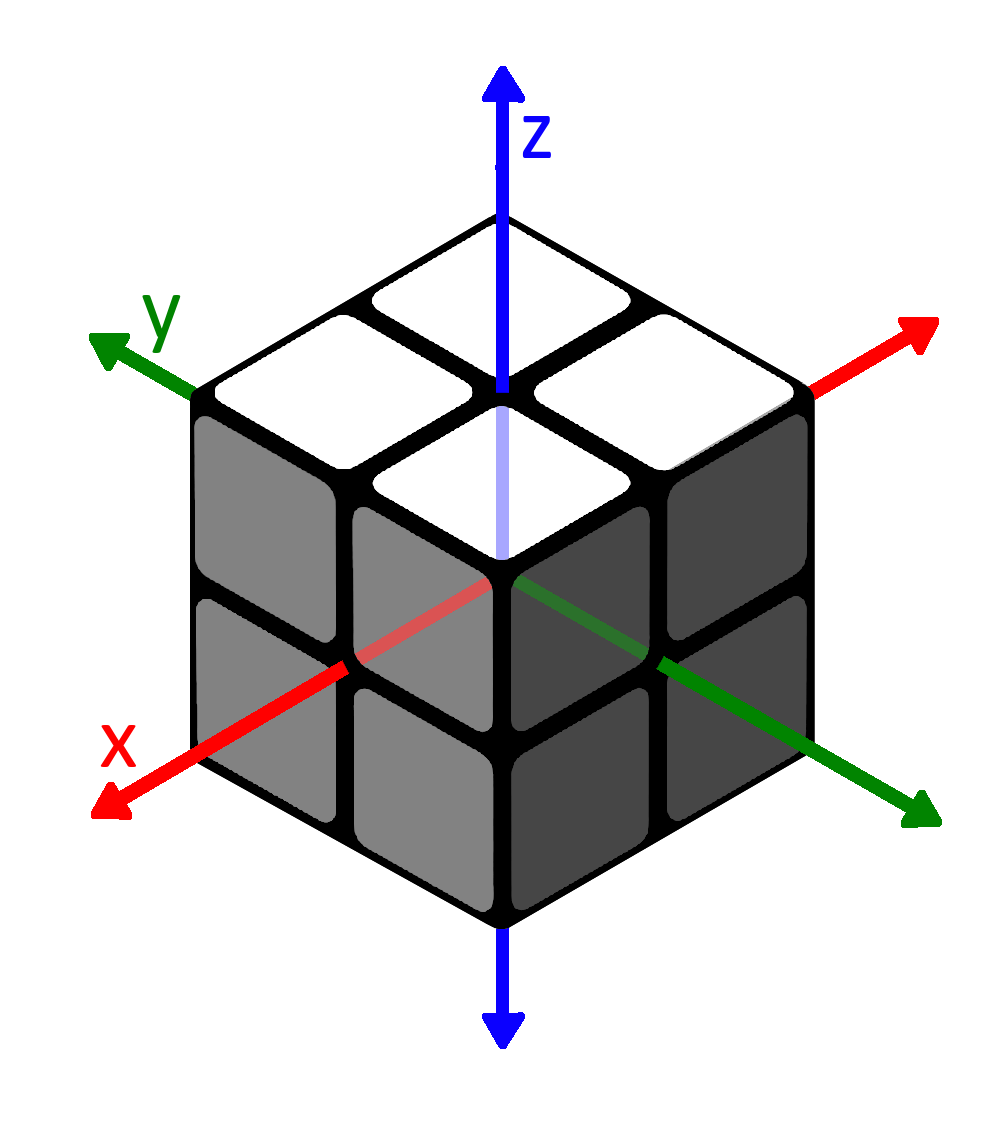
\includegraphics[scale=0.13]{Pfeile.png}
\caption[Würfel mit $x, y$ und $z$-Achsen]{Würfel mit $x, y$ und $z$-Achsen}
\label{Abbildung_Rotationsachsen}
\end{figure} 

Mit den Bezeichnungen der Achsen können für die möglichen Rotationen des Würfels Nachfolgekonfigurationen festgelegt werden. 
Dazu werden zuerst die einzelnen Rotationen des Würfels benannt. Dabei handelt es sich um 90$^\circ$-Drehungen.

\vspace*{1em}
\begin{adjustbox}{width=1\textwidth,center}
\begin{tabular}{cl}
\toprule
\textbf{Abkürzung} & \textbf{Beschreibung der Rotation} \\
\midrule
$Z_l$ & Rotation des Würfels um die $z$-Achse nach links (gegen den Uhrzeigersinn)\\

$Z_r$ & Rotation des Würfels um die $z$-Achse nach rechts (im Uhrzeigersinn)  \\

$Y_l$ & Rotation des Würfels um die $y$-Achse nach links (gegen den Uhrzeigersinn)\\

$Y_r$ & Rotation des Würfels um die $y$-Achse nach rechts (im Uhrzeigersinn)  \\

$X_l$ & Rotation des Würfels um die $x$-Achse nach links (gegen den Uhrzeigersinn)\\

$X_r$ & Rotation des Würfels um die $x$-Achse nach rechts (im Uhrzeigersinn) \\

$N_R$ & keine Rotation des Würfels \\
\bottomrule
\end{tabular} 
\end{adjustbox}
\vspace*{0.5em}


Die Rotationen sind zur besseren Anschaulichkeit nicht minimal definiert. Es gibt für jede Würfelseite nur vier Rotationsmöglichkeiten ($0^\circ, 90^\circ, 180^\circ, 270^\circ$), da immer um $90^\circ$ gedreht wird. Beispielsweise ist $Z_l$ das gleiche wie ${Z_r}^3$. Das bedeutet, das eine Drehung des Würfels um 90$^\circ$ nach links äquivalent zu drei 90$^\circ$ Drehungen des Würfels nach rechts ist.  Die Drehung nach links entspricht $0^\circ-90^\circ = 270^\circ$ während drei Drehungen nach rechts $0^\circ+90^\circ+90^\circ+90^\circ=270^\circ$ entsprechen.

Die Steine werden durch eine Rotation alle an einen neuen Platz gebracht. Anders als bei der Drehung der Ebenen, wo eine Auswahl der Steine die Position ändert, ändern hier alle Steine die Position. Die Folgekonfiguration des Würfels nach einer Rotation ist dann eine andere, äquivalente Konfiguration.

Anhand der Rotation $Z_r$, also einer Rotation des kompletten Würfels um die $z$-Achse um $90^\circ$ im Uhrzeigersinn, wird nun die Veränderung der Würfelpositionen erläutert. Der Würfel ist in Abbildung \ref{Abbildung_WürfelNachRotationUmZAchse} nach der Rotation $Z_r$ abgebildet.
\begin{figure}[H]
\centering
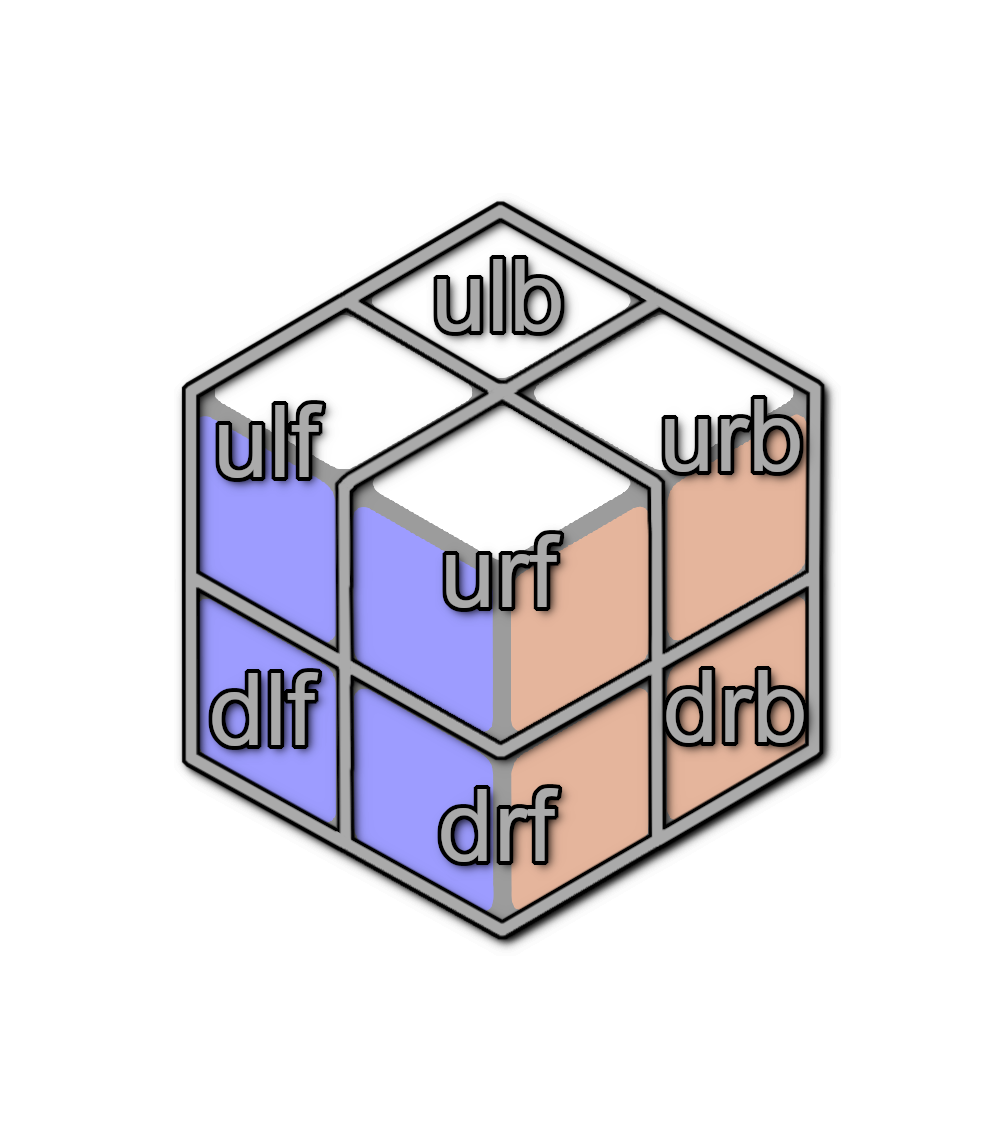
\includegraphics[scale=0.13]{auf_ulf.png}
\caption{Würfel nach Rotation um $z$-Achse}
\label{Abbildung_WürfelNachRotationUmZAchse}
\end{figure}
Die Permutationsfunktion der Rotationen wird im Folgenden $\delta$ genannt. Da bei den Rotationen alle Steine die Position wechseln, muss es für jede Rotation 8 Funktionen $\delta$ geben, für jeden Eckstein eine Funktion:
\begin{alignat*}{4}
& \delta_{Z_r}(\textit{urf}) = \textit{ulf} \ \ \ \ \ \ && \delta_{Z_r}(\textit{ulf}) = \textit{ulb} \ \ \ \ \ \ && \delta_{Z_r}(\textit{ulb}) = \textit{urb} \ \ \ \ \ \ && \delta_{Z_r}(\textit{urb}) = \textit{urf} \\
& \delta_{Z_r}(\textit{drf}) = \textit{dlf} \ \ \ \ \ \ && \delta_{Z_r}(\textit{dlf}) = \textit{dlb} \ \ \ \ \ \ \ && \delta_{Z_r}(\textit{dlb}) = \textit{drb} \ \ \ \ \ \ && \delta_{Z_r}(\textit{drb}) = \textit{drf}
\end{alignat*}

Die äquivalente Schreibweise in der Form $i \mapsto j$ lautet: 
\begin{alignat*}{4}
& \textit{urf} \mapsto \textit{ulf} \ \ \ \ \ \ \ \ && \textit{ulf} \mapsto \textit{ulb} \ \ \ \ \ \ \ \ && \textit{ulb} \mapsto \textit{urb} \ \ \ \ \ \ \ \ && \textit{urb} \mapsto \textit{urf} \\
& \textit{drf} \mapsto \textit{dlf} \ \ \ \ \ \ \ \ && \textit{dlf} \mapsto \textit{dlb} \ \ \ \ \ \ \ \ \ && \textit{dlb} \mapsto \textit{drb} \ \ \ \ \ \ \ \ && \textit{drb} \mapsto \textit{drf}
\end{alignat*}

In der Zykel-Schreibweise entspricht die Funktion $\delta_{Z_r}$ für die Rotation $Z_r$ dem folgenden Ausdruck:
\begin{align*}
\delta_{Z_r}=( \textit{urf} \ \textit{ulf} \ \textit{ulb} \ \textit{urb} )\ ( \textit{drf} \ \textit{dlf} \ \textit{dlb} \ \textit{drb}  )
\end{align*}
 

Die übrigen Rotationen können ebenfalls durch Funktionen $\delta$ in der Zykelschreibweise abgebildet werden. Die leere Rotation ist dabei die Identitätspermutation 1. Im Folgenden sind die Funktionen $\delta$ für alle Rotationen aufgelistet:
\begin{alignat*}{2}
& \delta_{Z_r} & = ( \textit{ulf} \ \textit{ulb} \ \textit{urb} \ \textit{urf})\ (\textit{dlf} \ \textit{dlb} \ \textit{drb} \ \textit{drf} )\\
& \delta_{Z_l} & = ( \textit{ulf} \ \textit{urf} \ \textit{urb} \ \textit{ulb})\ (\textit{dlf} \ \textit{drf} \ \textit{drb} \ \textit{dlb} )\\
& \delta_{Y_r} & = ( \textit{ulf} \ \textit{ulb} \ \textit{dlb} \ \textit{dlf})\ ( \textit{urf} \ \textit{urb} \ \textit{drb} \ \textit{drf} )\\
& \delta_{Y_l} & = ( \textit{ulf} \ \textit{dlf} \ \textit{dlb} \ \textit{ulb})\ ( \textit{urf} \ \textit{drf} \ \textit{drb} \ \textit{urb} )\\
& \delta_{X_r} & = ( \textit{ulf} \ \textit{urf} \ \textit{drf} \ \textit{dlf})\ ( \textit{urb} \ \textit{ulb} \ \textit{dlb} \ \textit{drb} )\\
& \delta_{X_l} & = ( \textit{ulf} \ \textit{dlf} \ \textit{drf} \ \textit{urf})\ (\textit{urb} \ \textit{ulb} \ \textit{dlb} \ \textit{drb} )\\
& \delta_{N_R} & = \ 1 \hspace*{14.1em}
\end{alignat*}

Da die Rotationen die Würfelkonfiguration in eine andere, äquivalente Würfelkonfiguration überführen, muss es neben der Permutationsfunktionen für die Veränderung der Steinposition auch Übergangsfunktionen für den Vektor $x$ geben, der die Ausrichtung der Steine darstellt. Die Funktionen $\gamma$ wurden für jeden Zug des Würfels ($U, D, R, L, F, B$) bereits in Abschnitt \ref{Abschnitt_AusrichtungDerSteine} definiert und beschrieben. Die Vektoreinträge der Steinausrichtungen werden dort mit den Funktionen $g, h$ und $i$ verändert.
\begin{align*}
g(x)=(x + 2) \hspace*{-0.5em} \mod 3 \ \ \ \ \ h(x) = (x+1) \hspace*{-0.5em} \mod 3 \ \ \ \ \ i(x)=x
\end{align*}

Die Überführungsfunktionen des Vektors $x$ werden im Folgenden $\beta$ genannt. Für jede der Rotationen gibt es eine Funktion $\beta$, die den Vektor in seinen Folgezustand überführt. Die Identitätsfunktion $i$ muss nicht mit aufgeführt werden. Die Funktionen $\beta$ für die Rotationen sind im Folgenden definiert:
\begin{align*}
\beta_{Z_r}  & \left( (x_1, x_2, x_3, x_4, x_5,x_6,x_7,x_8) \right)  \\
=  & \ (x_3, x_1, x_4, x_2, x_7, x_5, x_8, x_6) \\
\\
\beta_{Z_l}  &   \left( (x_1, x_2, x_3, x_4, x_5,x_6,x_7,x_8) \right)  \\
=  &  \ (x_2, x_4, x_1, x_3, x_6, x_8, x_5, x_7) \\
\\
\beta_{Y_r}  &  \left( (x_1, x_2, x_3, x_4, x_5,x_6,x_7,x_8)  \right) \\
=  & \ (h(x_3), g(x_4), g(x_7), h(x_8), g(x_1), h(x_2), h(x_5), g(x_6)) \\
\\
\beta_{Y_l}  &   \left( (x_1, x_2, x_3, x_4, x_5,x_6,x_7,x_8) \right)  \\
=  & \ (h(x_5), g(x_6), g(x_1), h(x_2),g(x_7),h(x_8),h(x_3),g(x_4)) \\
\\
\beta_{X_r}  &  \left( (x_1, x_2, x_3, x_4, x_5,x_6,x_7,x_8)  \right) \\
=  & \ (g(x_5), h(x_1), h(x_7), g(x_3), h(x_6), g(x_2), g(x_8),h(x_4)) \\
\\
\beta_{X_l}  &  \left( (x_1, x_2, x_3, x_4, x_5,x_6,x_7,x_8) \right)  \\
=  & \ (g(x_2), h(x_6), h(x_4),g(x_8), h(x_1), g(x_5), g(x_3), h(x_7)) 
\end{align*}

Wenn der Würfel nicht rotiert wird, bleibt der Vektor $x$ unverändert. Die Funktion $\beta$ für die leere Rotation $N_R$ ist im Folgenden definiert:
\begin{align*}
\beta_{N_R}  &  \left( (x_1, x_2, x_3, x_4, x_5,x_6,x_7,x_8) \right) \\
=  & \ (x_1, x_2, x_3, x_4, x_5,x_6,x_7,x_8)
\end{align*}

Es können auch mehrere Rotationen nacheinander ausgeführt werden. Die Funktionen $\delta$ und $\beta$ werden dann jeweils verschachtelt. Das erfolgt analog zu dem mehrfachen Ausführen von Zügen (s. Abschnitt \ref{Abschnitt_ZuegeAusfuehren}).

Beim Betrachten der Rotationen und der dazugehörigen Funktionen fällt auf, dass die Rotationen auch durch eine Kombination von Zügen definiert werden können. Die Rotationen entsprechen den folgenden Zügen:
\begin{alignat*}{3}
& Z_l && \Leftrightarrow \ \ &&  D U^{-1} \\
& Z_r && \Leftrightarrow &&  D^{-1} U \\
& Y_l && \Leftrightarrow && L R^{-1} \\
& Y_r && \Leftrightarrow && L^{-1} R  \\
& X_l && \Leftrightarrow && B F^{-1} \\
& X_r && \Leftrightarrow && B^{-1} F  \\
& N_R && \Leftrightarrow && N 
\end{alignat*}
Jede Rotation kann also durch die Ebenendrehungen von zwei gegenüberliegenden Würfelseiten dargestellt werden.



%
%
%
%
%
%
%
%
%
%=======================================================================================================
%
%
%
%
%
%
%
%
%
%

\subsection{Maximale Anzahl der Rotationen}
\label{Abschnitt_MaxAnzahlRotationen}

Die mehrfache Ausführung einer Rotation wird auch mit der Exponentenschreibweise geschrieben. 
Somit gilt für jede einelementige Rotation $T$ und Konfiguration $C$: 
\begin{align*}
\forall \ T \in \{{Z_r}, {Z_l}, {Y_r}, {Y_l}, {X_r}, {X_l} , N_R \} \ . \  C \cdot TTTT= C \cdot T^4=C \cdot N_R = C 
\end{align*} 
Dabei ist $N_R$ die leere Rotation und $T$ ist eine beliebige Rotation des Würfels. Es gilt somit für jede beliebige Rotation $T$:
\begin{align*}
T^{\hspace*{0.1em}0}=N_R
\end{align*}
Jede einelementige Rotation ist durch die Funktionen $\delta$ und $\beta$ definiert. Jede dieser Funktionen $\delta$ besteht in der Zykelschreibweise aus zwei 4-Zykeln. Diese Zykel befinden sich nach vier Ausführungen wieder in ihrem Ausgangszustand. Darauf wird in Abschnitt \ref{Abschnitt_OrdnungPermutationen} weiter eingegangen. Außerdem wird bei jeder Rotation der Vektor $x$ durch eine Funktion $\beta$ verändert. Der Vektor bleibt nach vierfachem Ausführen von $\beta$ unverändert. Der Beweis dazu findet sich in Anhang \ref{Anhang_Ausrichtungsfunktionen}.
Da alle vierfachen der einelementigen Rotationen (${Z_r}, {Z_l}, {Y_r}, {Y_l}, {X_r}, {X_l} , N_R$) keine Veränderung hervorrufen, kann der Exponent der Rotationen modulo 4 gerechnet werden: 
\begin{align*}
\forall \ T \in \{{Z_r}, {Z_l}, {Y_r}, {Y_l}, {X_r}, {X_l}, N_R \}, n \in \mathbb{N} \ . \ C \cdot T^n=C \cdot T^{n \hspace*{-0.5em} \mod 4}
\end{align*}

Anhand dieser Aussage ist ersichtlich, dass der Würfel sich nach mehreren Rotationen wieder seiner Ausgangsausrichtung nähern kann. Es gibt für die Roationen also eine maximale Tiefe, jede weitere Rotation bringt den Würfel wieder näher zu seiner Ausgangsrotation.
In diesem Abschnitt wird berechnet, wie oft der Würfel maximal um 90$^\circ$ rotiert werden muss, um zurück in die Ausgangsposition zu gelangen.

Da der Würfel 6 Seiten hat, die jeweils 4 verschiedene Ausrichtungen haben können, gibt es $4 \cdot 6 = 24$ verschiedene Rotationsmöglichkeiten für den Würfel. In Abbildung \ref{AbbildungWürfelRotationWeisseSeite} sind die vier verschiedenen Ausrichtungen des Würfels zu sehen, wenn die weiße Seite als obere Seite angenommen wird. In den Abbildungen wird von einem gelösten Würfel ausgegangen. Für die anderen fünf Seiten gibt es ebenfalls vier Möglichkeiten der Ausrichtung. Alle Rotationsmöglichkeiten sind in Anhang \ref{Anhang_RotationenDesWürfels} in Abbildung \ref{AbbildungWürfelRotationAlleSeiten} dargestellt.

\begin{figure}[H]
\centering
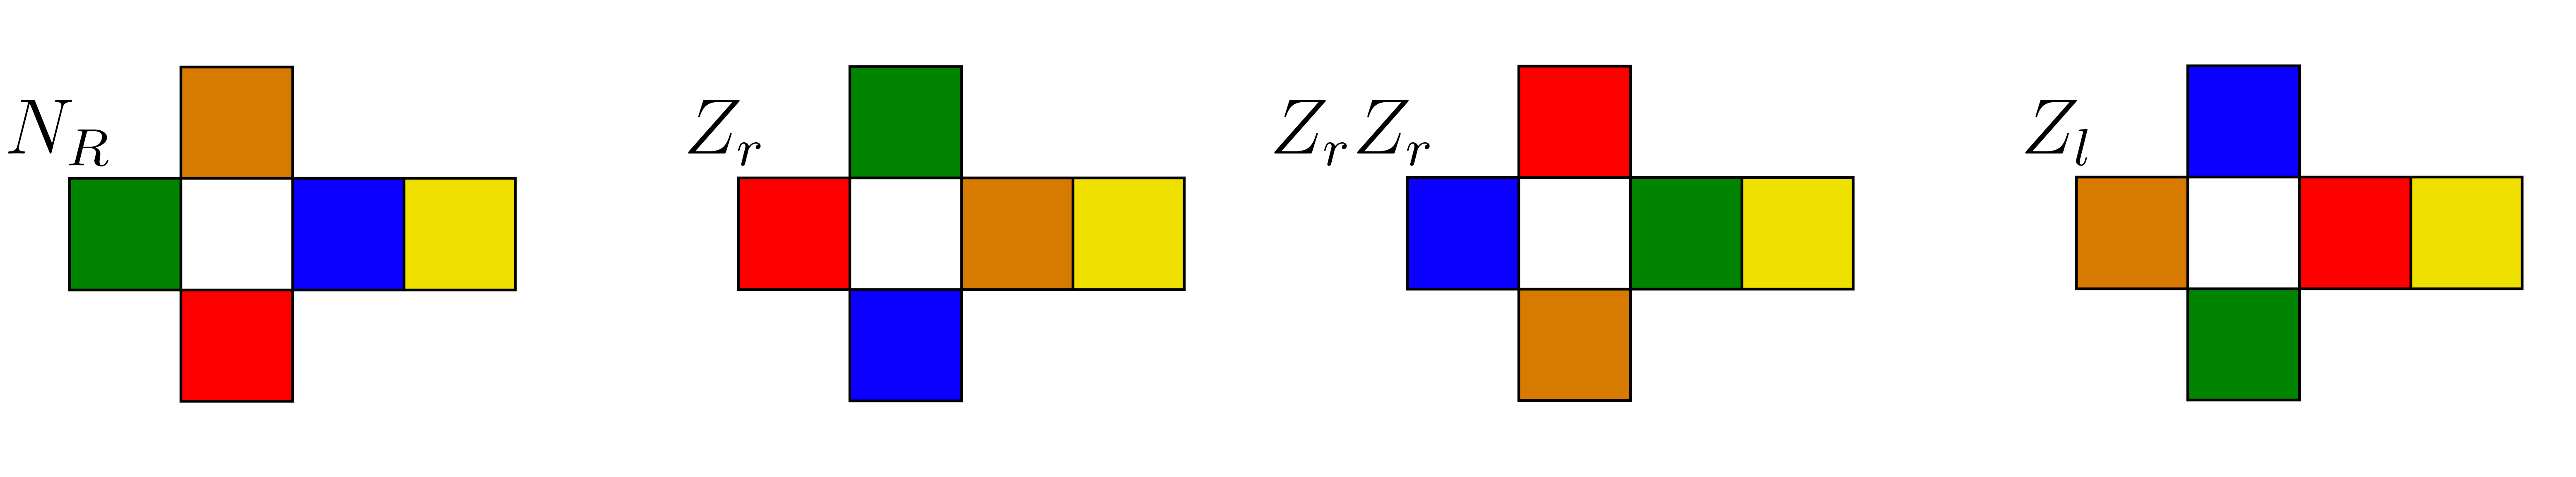
\includegraphics[scale=0.06]{RotationWeiss.png}
\caption{Rotationsmöglichkeiten des Würfels mit der weißen Seite oben}
\label{AbbildungWürfelRotationWeisseSeite}
\end{figure}

Neben den Abbildungen aller Rotationsmöglichkeiten des Würfels, befindet sich in Anhang \ref{Anhang_RotationenDesWürfels} eine Verknüpfungstafel, die alle Rotationen und die Verknüpfung dieser abbildet. Anhand dieser vollständigen Darstellung der Rotationsmöglichkeiten kann festgestellt werden, dass der Würfel maximal drei Rotationen von der Ausgangsausrichtung entfernt sein kann. Mit jeder weiteren Rotation nähert er sich seiner vorherigen Ausrichtung wieder an.





%
%
%
%
%
%
%
%
%
%
%=======================================================================================================
%
%
%
%
%
%
%
%
%
%

\subsection{Äquivalenzrelation der Züge}
\label{Abschnitt_ÄquivalenzrelationDerZüge}

Da der \Ttwo Würfel im Gegensatz zum \Tthree Würfel keine eindeutige Ausrichtung hat, werden in diesem Abschnitt Äquivalenzrelationen eingeführt, um die Rotationen des Würfels umzusetzen.
Damit eine Relation eine Äquivalenzrelationen ist, müssen die drei folgenden Eigenschaften gelten: Reflexivität, Symmetrie, Transitivität. In Abschnitt \ref{Abschnitt_Äquivalenrelationen} finden sich Definition und Erklärung.

In dem Fall des \Ttwo Würfels handelt es sich um eine Relation $\sim$ von zwei Zügen $Z_1, Z_2$ aus der Menge aller Züge $A_Z$ (ohne Rotationen). Dann ist die Relation $\sim$ eine Teilmenge von $A_Z \times A_Z$. 
Die Relation ist im Folgenden definiert: 

\begin{center}
\begin{tabular}{l l}
$Z_1 \sim Z_2 := \ $  & $Z_1$ \textit{und} $Z_2$ \textit{ergeben (mit optionaler Rotation) die gleiche }\\
\  & \textit{Würfelkonfiguration} \\
\end{tabular} 
\end{center}

Die Relation $\sim$ prüft zwei Züge $Z_1$ und $Z_2$ auf Gleichheit und berücksichtigt dabei gleichzeitig die Rotation des Würfels.

Daraus ergibt sich folgende Definition für alle Würfelkonfigurationen $C$ und $W$ als Element (oder Kombination von Elementen) aus $\{{Z_r}, {Z_l}, {Y_r}, {Y_l}, {X_r}, {X_l}, N_R\}$. Dabei stellt $N_R$ die leere Rotation dar -- das entspricht keiner Rotation des Würfels. 
\begin{align*}
Z_1 \sim Z_2 :\Leftrightarrow \ C \cdot Z_1 = C \cdot WZ_2
\end{align*}

Somit ergibt sich beispielsweise $F \sim L \Leftrightarrow C \cdot F = C \cdot Z_rL$, da eine Drehung der vorderen Ebene und eine Drehung des Würfels nach links mit einer Drehung der linken Ebene eine äquivalente Würfelkonfiguration ergeben. Der Würfel ist dann lediglich verschieden ausgerichtet. 
In Abbildung \ref{Abbildung_GelöstnachFnachZL} ist dieses Beispiel grafisch dargestellt: Links befindet sich der gelöste Würfel, in der Mitte der Würfel nach dem Zug $F$ und rechts der Würfel nach dem Zug $Z_rL$. Die beiden rechten Würfel sind in der äquivalenten Konfigurationen, aber anders gedreht.
\begin{figure}[h]
\centering
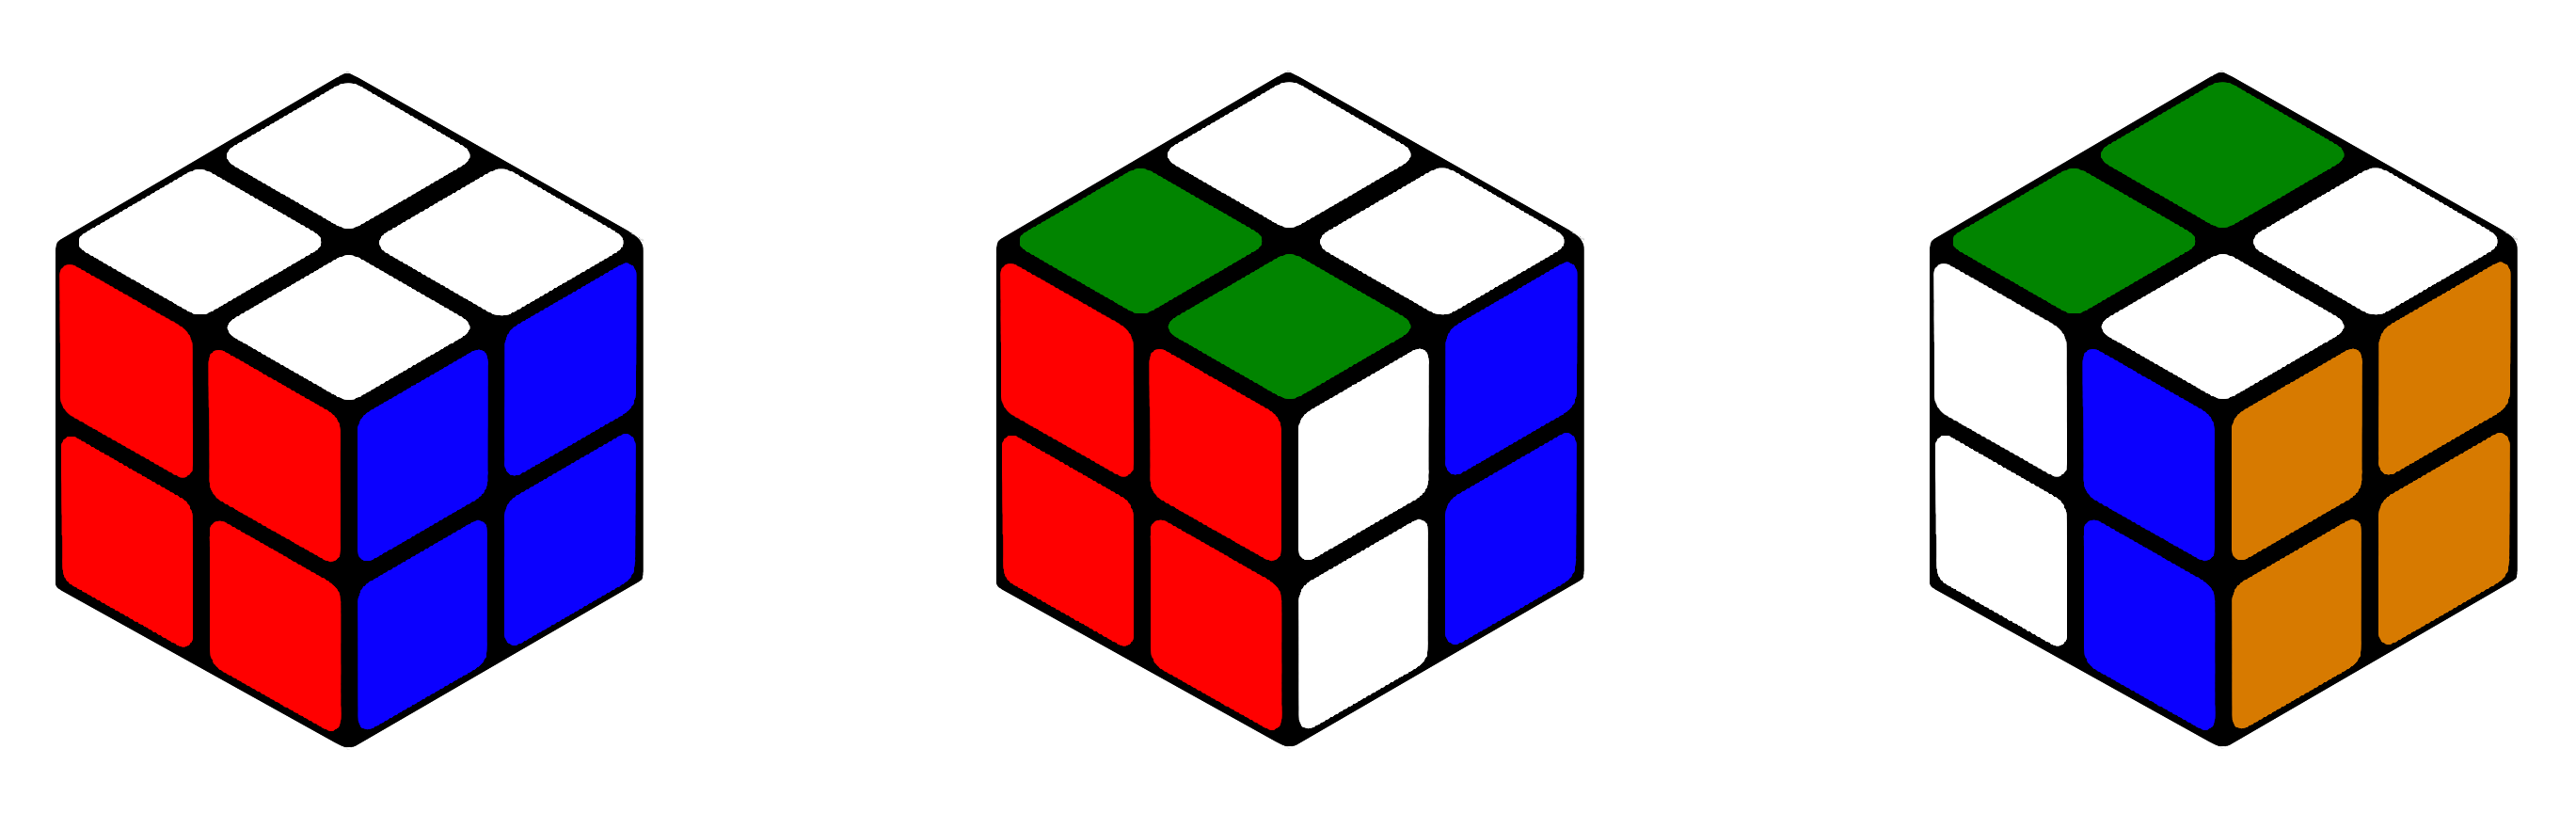
\includegraphics[scale=0.15]{3_wuerfel.png}
\caption[Würfel gelöst, nach Zug $F$ und nach $Z_rL$]{Würfel gelöst (links), nach Zug $F$ (Mitte) und nach $Z_rL$(rechts)}
\label{Abbildung_GelöstnachFnachZL}
\end{figure}

Damit $\sim$ eine Äquivalenzrelation ist, müssen Reflexivität, Symmetrie und Transitivität gelten. Diese Eigenschaften werden im Folgenden für die Relation $\sim$ gezeigt.

\begin{description}


\item [Reflexivität] \ \\
Für die Reflexivität muss $Z \sim Z$ für alle Züge gelten. Jeder Zug muss dafür zu sich selbst in Relation stehen.
\begin{align*}
Z_1 \sim_R Z_2 : & \Leftrightarrow C \cdot Z_1 = C \cdot WZ_2
\end{align*}
Um zu zeigen, dass $Z_1$ und $Z_2$ äquivalent sind, wird die Rotation $W$ als $N_R$ gewählt, so dass keine Rotation ausgeführt wird.
\begin{align*}
Z_1 \sim Z_2 : & \Leftrightarrow  C \cdot Z_1 = C \cdot WZ_2 \\
\ & \Leftrightarrow C \cdot Z_1=C \cdot N_R Z_2 \\
\ & \Leftrightarrow C \cdot Z_1 = C \cdot Z_2
\end{align*}
Bei $Z_1 \sim Z_2$ mit $W=N_R$ sind die Züge $Z_1$ und $Z_2$ immer äquivalent, da sie bei gleicher Startkonfiguration die gleiche Folgekonfiguration des Würfels erzeugen. Es gilt somit die Reflexivität für die Relation $\sim$.

\item [Symmetrie] \ \\
Für die Symmetrie muss folgendes gelten: Aus $Z_1 \sim Z_2$ folgt $Z_2 \sim Z_1$.
\begin{align*}
Z_1 \sim Z_2 & \Rightarrow Z_2 \sim Z_1 \\
mit \ Z_1 \sim Z_2 : & \Leftrightarrow  C \cdot  Z_1 = C \cdot  WZ_2 \\
\Leftrightarrow C \cdot  Z_1 = C \cdot  W_1 Z_2 & \Rightarrow C \cdot  Z_2 = C \cdot  W_2 Z_1
\end{align*}
$Z_2 \sim Z_1$ muss gelten, wenn $Z_1 \sim Z_2$ gilt. Da $Z_1 \sim Z_2$ gilt, sind die Züge $Z_1$ und $Z_2$ mit optionaler Rotation gleich. 
\begin{description}

\item[Fall 1:] 
Die optionale Rotation $W$ entspricht der leeren Rotation $N_R$. Dann führen die Züge $Z_1$ und $Z_2$ zu derselben Folgekonfiguration des Würfels und werden als gleich angesehen:
\begin{alignat*}{2}
& Z_1 \sim Z_2 && \Rightarrow Z_2 \sim Z_1 \textit{ mit }  W = N_R \\ 
\Leftrightarrow \  & C \cdot  Z_1 = C \cdot  N_R Z_2 \ && \Rightarrow C \cdot  Z_2 = C \cdot  N_R Z_1 \\
\Leftrightarrow \  & C \cdot  Z_1 = C \cdot  Z_2 && \Rightarrow C \cdot  Z_2 = C \cdot  Z_1 
\end{alignat*}
Folglich gilt die Symmetrie für $W = N_R$.

\item[Fall 2:]
Die optionale Rotation besteht aus einem oder mehreren Elementen aus $\{{Z_r}, {Z_l}, {Y_r}, {Y_l}, {X_r}, {X_l}, N_R\}$.
Die Symmetrie gilt, wenn $W_2$ das Inverse von $W_1$ ist. Das Inverse einer Rotation ist die Rotation um die gleiche Achse, aber in die andere Richtung. 
Das Inverse von $W$ wird als $W^{-1}$ geschrieben. 
Da es sich bei den Rotationen (so wie bei den Ebenendrehungen) um $90^\circ$-Drehungen handelt, entspricht das inverse Element einer Rotation der dreifachen Ausführung dieser. 
Es gilt dann:
\begin{align*}
\forall  \ W \in \{{Z_r}, {Z_l}, {Y_r}, {Y_l}, {X_r}, {X_l}, N_R\} \ . \ W^{-1} = WWW = W^3
\end{align*}
Da die Rotationen zur besseren Übersichtlichkeit nicht minimal definiert wurden, sind in der folgenden Tabelle alle Rotationen uns die dazugehörigen Inversen abgebildet:

\begin{center}
\begin{tabular}{lcccccc}
Rotation $W$ & ${Z_r}$ & ${Z_l}$ &  ${Y_r}$ & ${Y_l}$ & ${X_r}$ & ${X_l}$  \\
\hline
Inverses \hspace*{0.1em} $W^{-1}$ & ${Z_l}$ & ${Z_r}$ &  ${Y_l}$ & ${Y_r}$ & ${X_l}$ & ${X_r}$  \\
\end{tabular} 
\end{center}


Wenn sich eine Rotation aus mehreren Elementen aus $\{{Z_r}, {Z_l}, {Y_r}, {Y_l}, {X_r}, {X_l}, N_R\}$ zusammensetzt, muss das hintere Element zuerst invertiert werden. Die Definition ist analog zu der Definition des inversen Elements der Züge aus $\Gtwo.$ Diese Definition findet sich in Abschnitt \ref{Abschnitt_WürfelAlsGruppe}.
 
Es gilt: 
\begin{align*}
C \cdot  Z_1 = C \cdot  W Z_2 & \Rightarrow C \cdot  Z_2 = C \cdot  W^{-1} Z_1
\end{align*}
Das gilt, da durch $W^{-1}$ der Würfel in die entgegengesetzte Richtung rotiert wird und die Züge somit wieder die gleiche Würfelkonfiguration ergeben.

\end{description}

Folglich gilt die Symmetrie für $\sim$.


\item [Transitivität] \ \\
Es muss gelten: Aus $Z_1 \sim Z_2$ und $Z_2 \sim Z_3$ folgt $Z_1 \sim Z_3$.
\begin{alignat*}{3}
& Z_1 \sim Z_2 && \wedge Z_2 \sim Z_3 && \Rightarrow Z_1 \sim Z_3 \\
\Leftrightarrow \ & C \cdot  Z_1 = C \cdot  W_1Z_2 \ && \wedge C \cdot  Z_2 = C \cdot  W_2Z_3 \ && \Rightarrow C \cdot  Z_1 = C \cdot  W_3Z_3
\end{alignat*}
Da die Züge $Z_1$ und $Z_2$ mit der Rotation $W_1$ die gleiche Würfelkonfiguration ergeben, und die Züge $Z_2$ und $Z_3$ nach der Rotation $W_2$ auch die gleiche Würfelkonfiguration ergeben, gilt das auch für die beiden Züge $Z_1$ und $Z_3$ nach der Rotation $W_3=W_1W_2$, da dann alle nötigen Rotationen durchgeführt wurden:
\begin{alignat*}{3}
C \cdot  Z_1 = C \cdot  W_1Z_2 \ && \wedge C \cdot  Z_2 = C \cdot W_2Z_3 \ && \Rightarrow C \cdot  Z_1 = C \cdot W_1W_2Z_3 
\end{alignat*}

Die Transitivität gilt somit für die Relation $\sim$.

\end{description}

Da die Eigenschaften der Reflexivität, Symmetrie und Transitivität für die Relation $\sim$ gelten, handelt es sich um eine Äquvalenzrelation.




%
%
%
%
%
%
%
%
%
%
%=======================================================================================================
%
%
%
%
%
%
%
%
%
%


\subsection{Äquivalenzklassen der Züge} 

\label{Abschnitt_ÄquivalenzklassenDerZüge}

Äquivalenzklassen und Faktormengen wurden in Abschnitt \ref{Abschnitt_FaktormengenUndÄquivalenzklasse} eingeführt. In diesem Abschnitt werden die Äquivalenzklassen der Äquivalenzrelation $\sim$ auf der Menge aller Züge $A_Z$ definiert und damit eine Faktormenge gebildet, die diese Äquivalenzklassen enthält. Jede Äquivalenzklasse ist definiert als:
\begin{align*}
[Z] := \{ Y \in A_Z \mid Y \sim Z \} \subseteq A_Z
\end{align*}
Demnach enthält jede Äquivalenzklasse $[Z]$ alle Züge der Menge $A_Z$, die mit der Äquivalenzrelation $\sim$ äquivalent zu $Z$ sind. Dabei ist $[Z]$ eine Teilmenge von $A_Z$.  Alle äquivalenten Elemente einer Äquivalenzklasse $[Z]$ werden als Repräsentanten dieser Äquivalenzklasse bezeichnet. So sind die Züge $R$ und $RRRRR$ beispielsweise Repräsentanten der Äquivalenzklasse $[R]$, da die Züge $R$ und $RRRRR$ mit der Äquivalenzrelation $\sim$ äquivalent zu $R$ sind.

Die Gleichheit zweier Züge wurde durch die Äquivalenzrelation $\sim$ definiert. Dabei gelten zwei Züge als äquivalent, wenn sie bei derselben Startkonfiguration mit optionaler Rotation des Würfels zur gleichen Folgekonfiguration führen. Daher sind zwei gleiche Züge $Z_1, Z_2 \in A_Z$ immer Repräsentanten der gleichen Äquivalenzklasse. Umgekehrt sind zwei Züge $Z_1, Z_2 \in A_Z$, die nicht zur gleichen Folgekonfiguration führen, Repräsentanten unterschiedlicher Äquivalenzklassen.
Daraus resultiert, dass zwei verschiedene Äquivalenzklassen keine äquivalenten Züge enthalten, da alle äquivalenten Züge in genau einer Äquivalenzklasse sind. 

Die Faktormenge $A_Z / \sim$ wird im weiteren Verlauf der Arbeit $\Gtwo$ genannt. Sie enthält die Äquivalenzklassen aller Würfelzüge, ohne dabei gleiche Züge oder Würfelrotationen doppelt zu enthalten.
Die Elemente von $\Gtwo$ sind alle Äquivalenzklassen bezüglich der Äquivalenzrelation $\sim$. Es gilt demnach:
\begin{align*}
\Gtwo := \{[Z] \mid Z \in A_Z \}
\end{align*}
$\Gtwo$ enthält somit die Äquivalenzklassen aller möglichen Züge des Würfels. 
Im weiteren Verlauf dieser Arbeit werden die eckigen Klammern der Äquivalenzklassen in $\Gtwo$ weggelassen, um die Notation zu vereinfachen.

Zwei Äquivalenzklassen bzw. deren Repräsentanten können durch den Operator $\circ$ verknüpft werden. Die Züge werden dann nacheinander (von links) ausgeführt. Das Ausführen der Züge erfolgt bei den Äquivalenzklassen der Züge äquivalent zu dem in Abschnitt \ref{Abschnitt_ZuegeAusfuehren} definierten Ausführen von Zügen.

%
%
%
%
%
%
%
%
%
%=======================================================================================================
%
%
%
%
%
%
%
%
%
%

\subsection{\Ttwo Zauberwürfel als Gruppe} 
 \label{Abschnitt_WürfelAlsGruppe}

Im Folgenden wird die Definition der Gruppe des \Tthree Würfels aus \textit{Group Theory and the Rubik's Cube}  von Janet Chen \cite{JC} als Gruppe des \Ttwo Würfels umgesetzt. Die Gruppe des \Ttwo Würfels heißt im Folgenden $(\Gtwo, \circ)$. 
Grundlagen und Definition der Gruppe wurden in Abschnitt \ref{Abschnitt_Gruppe} erklärt.


Die Trägermenge $\Gtwo$ der Gruppe wurde in Abschnitt \ref{Abschnitt_ÄquivalenzklassenDerZüge} definiert. Sie besteht aus den Äquivalenzklassen aller möglichen Zügen des Würfels. Äquivalente Züge sind dabei Repräsentanten der gleichen Äquivalenzklasse.


Der Operator $\circ$ ist als Konkatenation zweier Züge definiert. Seien $Z_1$ und $Z_2$ zwei Züge in $\Gtwo$. Dann bedeutet $Z_1 \circ Z_2$, dass zuerst $Z_1$ und dann $Z_2$ ausgeführt wird. $Z_1 \circ Z_2$ kann auch als $Z_1Z_2$ geschrieben werden.

Im Folgenden wird gezeigt, dass $(\Gtwo, \circ)$ eine Gruppe ist, indem $(\Gtwo, \circ)$ bezüglich der Gruppenkriterien untersucht wird:


\begin{description}
\item [Abgeschlossenheit] \ \\
$\forall \ Z_1,Z_2 \in \Gtwo \  . \   (Z_1 \circ Z_2) \in \Gtwo $ 


Seien $Z_1$ und $Z_2$ Züge und somit Elemente aus $\Gtwo$. Dann ist auch $Z_1 \circ Z_2$ ein Element aus $\Gtwo$. Die Menge $\Gtwo$ enthält Äquivalenzklassen. Diese wurden in Abschnitt \ref{Abschnitt_ÄquivalenzklassenDerZüge} mit den Elementen aus der unendlichen Menge aller Züge $A_Z$ definiert. Es sind somit alle Elemente der Menge $A_Z$ Repräsentanten der Äquivalenzklassen in $\Gtwo$. Eine Verknüpfung zweier Züge ist auch ein Zug aus $A_Z$. Somit ist $Z_1 \circ Z_2$ ebenfalls Repräsentant einer Äquivalenzklasse in $\Gtwo$. Die Gruppe $(\Gtwo, \circ)$ ist folglich unter dem Operator $\circ$ abgeschlossen.
 
Mit den Ergebnissen aus Abschnitt \ref{Abschnitt_MächtigkeitVonG} kann die Abgeschlossenheit von $(\Gtwo, \circ)$ auch anders begründet werden: In $\Gtwo$ findet sich zu jeder validen Würfelkonfiguration ein Zug, mit dem diese erreicht werden kann und jede Verknüpfung von zwei validen Zügen führt zu einer validen Würfelkonfiguration. Daher gilt die Abgeschlossenheit bei der Gruppe $(\Gtwo, \circ)$.


\item [Assoziativität] \ \\
$\forall \ Z_1,Z_2,Z_3 \in \Gtwo \ . \ (Z_1 \circ Z_2) \circ Z_3 = Z_1 \circ (Z_2 \circ Z_3)$ 


Um die Assoziativität zu zeigen, wird eine Schreibweise für das Ausführen der Züge eingeführt. Ein beliebiger, fester Stein im Würfel wird hier $s$ genannt. Beim Ausführen eines Zuges $Z$ wird nun $Z(s)$ geschrieben, um die neue Position des Steines zu erhalten. Die Positionen sind (wie oben beschrieben) 3-Buchstaben-Kürzel, bestehend aus $u, d, r, l, f, b$. 

Bei der Betrachtung von $Z_1 \circ Z_2 $, wird zuerst $Z_1$ und dann $Z_2$ ausgeführt. $Z_1(s)$ bewegt den Stein $s$ zu der Position $Z_1(s)$. Der Zug $Z_2$ bewegt den Stein dann zu der Position $Z_2(Z_1(s))$. Folglich gilt $Z_1 \circ Z_2 = Z_2(Z_1(s))$. 


Nun muss noch $(Z_1 \circ Z_2) \circ Z_3 = Z_1 \circ (Z_2 \circ Z_3)$ gezeigt werden. Dafür wird gezeigt, dass sich $(Z_1 \circ Z_2) \circ Z_3$ und $Z_1 \circ (Z_2 \circ Z_3)$ beide zu $Z_3(Z_2(Z_1(s))$ umformen lassen: 
\begin{align*}
& (Z_1 \circ Z_2) \circ Z_3  \\
\Leftrightarrow (&(Z_1 \circ Z_2) \circ Z_3)(s) \\
= & Z_3(Z_1 \circ Z_2)(s)) \\
= & Z_3(Z_2(Z_1(s)))  
\\
\\
&Z_1 \circ (Z_2 \circ Z_3) \\
\Leftrightarrow (&Z_1 \circ (Z_2 \circ Z_3))(s) \\
= (&Z_2 \circ Z_3)(Z_1(s)) \\
= \ \ & Z_3(Z_2(Z_1(s)))  
\end{align*}
Somit ist $(\Gtwo, \circ)$ assoziativ.

\item [Existenz eines neutralen Elements $\boldsymbol{N}$] \ \\
$\exists \ N \in \Gtwo \  \forall Z \in \Gtwo \ . \ N \circ Z = Z \circ N = Z$ 


Das neutrale Element $N$ muss eine Äquivalenzklasse aus der Menge der Züge $\Gtwo$ sein. Für alle Züge $Z \in \Gtwo$ muss gelten: $N \circ Z = Z \circ N = Z$. Wird der Zug $Z$ mit dem neutralen Element $N$ verknüpft, so bleibt er unverändert. Betrachtet man den physischen Würfel, so ist das neutrale Element der Gruppe $(\Gtwo, \circ)$ der leere Zug. Es werden dabei keine der Ebenen des Würfels gedreht. Wenn ein Zug $Z$ ausführt wird und dann der Zug $N$, bedeutet das \textit{erst $Z$ ausführen und dann nichts}, was das gleiche ist wie \textit{$Z$ auszuführen}. 

Wenn das auf das mathematischen Modell des Würfels übertragen wird, ändert sich die Würfelkonfiguration durch das Ausführen von $N$ nicht. Die Permutationsfunktion für das  neutrale Element ist dann $\sigma_N=1$ und die Übergangsfunktion $\gamma_N$ des Vektors $x$ ist $\gamma_N(x)=x$. Der Vektor wird dabei unverändert zurückgegeben.


Wird beispielsweise eine einzelne Ebene viermal am Stück gedreht, befindet sich der Würfel wieder in der Ausgangskonfiguration. Somit gilt beispielsweise $RRRR=R^4=N$. Das gilt analog für alle einelementigen Züge des Würfels.
Die vierfachen Ausführungen der Grundzüge sind alle als Repräsentanten des leeren Zuges in der Äquivalenzklasse von $N$ enthalten.
Für jeden beliebigen Zug $Z$ aus $\Gtwo$ gilt somit auch $Z^0=N$, da die Würfelkonfiguration bei nullfacher Ausführung eines Zuges unverändert bleibt.

Das neutrale Element $N$ von $(\Gtwo, \circ)$ ist somit die Äquivalenzklasse des leeren Zuges.


\item [Existenz eines inversen Elements $\boldsymbol{Z^{-1}}$] \ \\
$\forall \  Z \in \Gtwo \ \exists \  Z^{-1} \in \Gtwo \ .  \ Z \circ Z^{-1} = Z^{-1} \circ Z = N$  


Jeder Zug $Z$ überführt eine Würfelkonfiguration in eine Folgekonfiguration. 
Das passiert durch eine Permutationsfunktion $\sigma$ und eine Übergangsfunktion $\gamma$ für den Vektor $x$. 
Betrachtet man den physischen Würfel, so wird auffallen, dass man die einzelnen Ebenen auch gegen den Uhrzeigersinn drehen kann und somit eine Ebenendrehung invertiert. Eine Ebenendrehung um $90^\circ$ gegen den Uhrzeigersinn entspricht einer Ebenendrehung um $270^\circ$ im Uhrzeigersinn. Die Funktionen $\sigma$ und $\gamma$ sind dabei gleich.
Die Inversen der einzelnen Ebenendrehungen werden somit folgendermaßen definiert:
\begin{align*}
\forall \ Z \in \{U, D, F, B, L, R\} \ . \ Z^{-1} = ZZZ = Z^3
\end{align*}
Soll ein Zug invertiert werden, der aus mehreren Grundzügen besteht, so muss das hintere Element zuerst invertiert werden. Bei einem Zug $Y$ der Länge $n$ wird zuerst der $n$-te Grundzug $Z_n$ invertiert, indem er in $Z_nZ_nZ_n$ überführt wird. Daraufhin werden die weiteren Elemente des kompletten Zuges von hinten invertiert. Im Folgenden ist das inverse Element jedes Zuges definiert. Dabei ist $n \in \mathbb{N}$ und $Z_i$ repräsentiert alle Teilzüge $Z_1$ - $Z_n$, aus denen sich der Zug $Y$ zusammensetzt.
\begin{align*}
\forall \ Y \in \Gtwo, Y & = (Z_1 \circ Z_2 \circ ... \circ Z_n), Z_{i} \in \{U, D, F, B, L, R\} \ . \  \\
Y^{-1} & = {Z_n}^{-1} \circ {Z_{n-1}}^{-1} \circ ... \circ {Z_1}^{-1} 
\end{align*}
Das kann mit der oben beschriebenen Definition von $Z^{-1}$ (mit $Z \in \{U, D, F, B, L, R\} $) folgendermaßen umgeformt werden:
\begin{align*}
Y^{-1} & = {Z_n}^{-1} \circ {Z_{n-1}}^{-1} \circ ... \circ {Z_1}^{-1} \\
& = Z_nZ_nZ_n \circ Z_{n-1}Z_{n-1}Z_{n-1} \circ ... \circ Z_1Z_1Z_1 \\
& = {Z_n}^3 \circ {Z_{n-1}}^3 \circ ... \circ {Z_1}^3 \\
& = {Z_n}^3{Z_{n-1}}^3 ...  {Z_1}^3 \\
\end{align*}
Mit diesen Ausdrücken sind die inversen Elemente für jeden Zug aus $\Gtwo$ definiert.



\end{description}
Somit ist $(\Gtwo, \circ)$ eine Gruppe, da die vier Gruppenaxiome erfüllt sind. 


$(\Gtwo, \circ)$ ist keine kommutative Gruppe, da beispielsweise eine Rotation der rechten Ebene im Uhrzeigersinn ($R$) und eine Rotation der vorderen Ebene im Uhrzeigersinn ($F$) in umgekehrter Reihenfolge ein anderes Ergebnis haben. Dieses Beispiel ist in Abbildung \ref{Abbildung_WürfelNachFRundRF} grafisch dargestellt oder kann händisch an einem Würfel ausprobiert werden.
\begin{figure}[H]
\centering
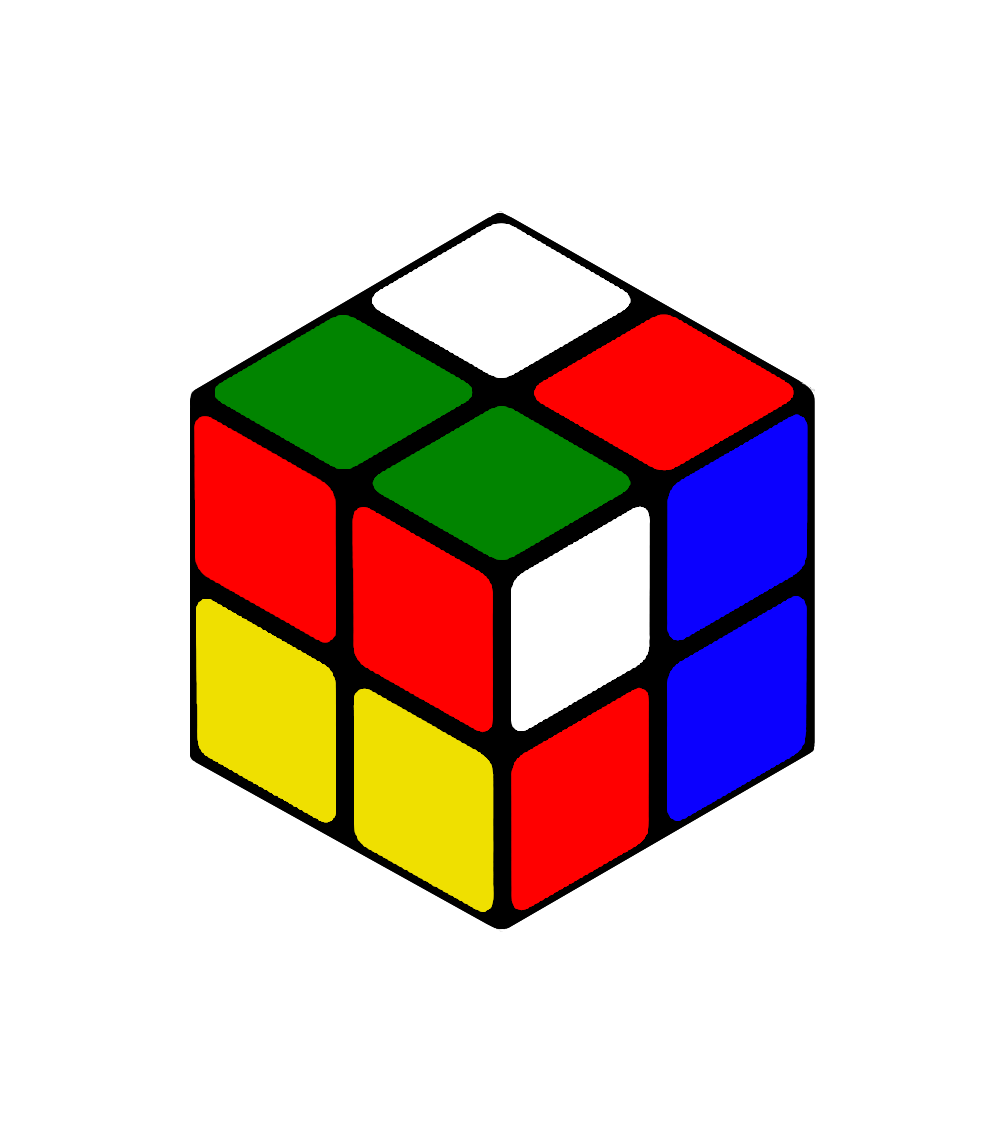
\includegraphics[scale=0.1]{RF.png}
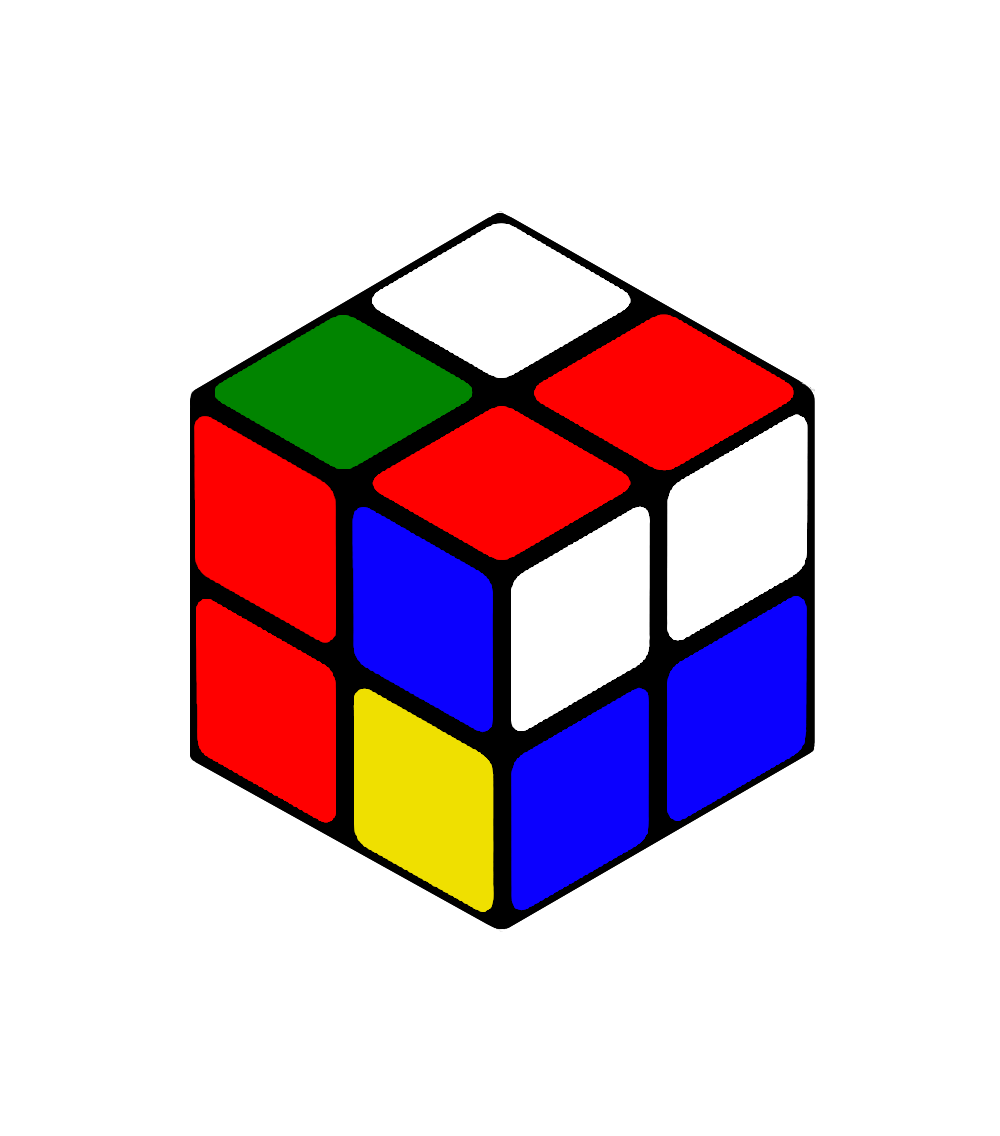
\includegraphics[scale=0.1]{FR.png}
\caption[Würfel nach Zügen $FR$ (links) und $RF$ (rechts)]{Würfel nach Zügen $FR$(links) und $RF$(rechts)}
\label{Abbildung_WürfelNachFRundRF}
\end{figure}
%Außerdem wäre das Lösen des Würfels trivial, wenn die Kommutativität gelten würde. \cite{TD} Die Reihenfolge der gedrehten Ebenen wäre dann irrelevant und es müsste lediglich die Anzahl beachtet werden. 
%Es gilt dementsprechend nicht $\forall \  Z_1, Z_2 \in \Gtwo. Z_1 \circ Z_2 = Z_2 \circ Z_1$ und der $\circ$-Operator der Gruppe ist somit nicht kommutativ. 

%
%
%
%
%
%
%
%
%
%
%=======================================================================================================
%
%
%
%
%
%
%
%
%
%
\subsection{Züge als Gruppenoperation}

Im Folgenden wird eine Gruppenoperation beschrieben, die eine Würfelkonfiguration durch das Ausführen eines Zuges auf eine neue Würfelkonfiguration abbildet. Bei Gruppenoperationen beeinflussen die Elemente einer Gruppe eine Menge. In diesem Fall beeinflussen die Züge des Würfels die Konfiguration des Würfels. Es handelt sich um eine Rechtsoperation, da die Elemente der Gruppe von rechts auf den Elementen der Menge operieren. Die Rechtsoperation wurde in Abschnitt \ref{Abschnitt_Gruppenoperation} definiert.

Bei $\Gtwo$ handelt es sich um die Trägermenge und $M_C$ ist die Menge aller Konfigurationen. Der Punktoperator ist im Folgenden definiert:
\begin{align*}
\cdot: M_C \times \Gtwo \rightarrow M_C
\end{align*} 
Wird eine Konfiguration $C=(\sigma, x)$ aus der Menge der Konfigurationen $M_C$ durch das Ausführen eines Zuges $Z \in \Gtwo$ in eine neue Konfiguration überführt, so wird diese Folgekonfiguration als $(C \cdot Z) \in M_C$ geschrieben.
Die folgenden beiden Eigenschaften müssen bei der Rechtsoperation gelten:

\begin{description}
\item [$\boldsymbol{C \cdot N = C}$ für alle $\boldsymbol{C \in M_C}$ und das neutrale Element $\boldsymbol{N \in \Gtwo}$] 
\ \\
Wenn der leere Zug $N$ ausgeführt wird, wird die Konfiguration des Würfels nicht verändert. Der leere Zug überführt die Konfiguration mit $\sigma_N=1$ und $\gamma_N(x)=x$. Sowohl die Permutationsfunktion $\sigma$ als auch der Vektor $x$ bleiben bei Ausführung des leeren Zuges $N$ unverändert. Daher gilt:
\begin{align*}
 C \cdot N 
\Leftrightarrow \ \ & (\sigma, x) \cdot  N \\
= \ \ & (\sigma_N \diamond \sigma, \gamma_N(x)) \\
= \ \ & (\sigma, x) \\
= \ \ & C
\end{align*}

\item [$\boldsymbol{C \cdot (Z_1 \circ Z_2) = (C \cdot Z_1) \cdot Z_2}$ für alle $\boldsymbol{Z_1, Z_2 \in \Gtwo}$ und $\boldsymbol{C \in M_C}$]
\ \\
Sei $C$ eine Konfiguration des Würfels. Wird von der Konfiguration $C$ ausgehend der Zug $Z_1 \in \Gtwo$ ausgeführt, ist die neue Konfiguration des Würfels $C \cdot Z_1$. Wenn nun noch ein weiterer Zug $Z_2 \in \Gtwo$ ausgeführt wird, ist die neue Konfiguration des Würfels $(C \cdot Z_1) \cdot Z_2$. 
Es wurde demnach mit Konfiguration $C$ gestartet und die Züge $Z_1$ und $Z_2$ wurden ausgeführt. Das kann folgendermaßen umgeformt werden:
\begin{align*}
& (C \cdot Z_1) \cdot Z_2 \\
\Leftrightarrow \ & C \cdot Z_1Z_2 \\
\Leftrightarrow \ & C \cdot (Z_1 \circ Z_2)
\end{align*}
Die neue Konfiguration kann demnach auch als $C \cdot (Z_1 \circ Z_2)$ geschrieben werden und somit gilt $(C \cdot Z_1) \cdot Z_2 = C \cdot (Z_1 \circ Z_2)$. 
\end{description}

Da beide Eigenschaften gelten, handelt es sich um eine Rechtsoperation. Die Züge der Gruppenträgermenge operieren von rechts auf der Menge aller Würfelkonfigurationen.

%
%
%
%
%
%
%
%=======================================================================================================
%
%
%
%
%

\subsection{Ordnung der Permutationen}
 \label{Abschnitt_OrdnungPermutationen}

In den Abschnitten \ref{Abschnitt_GleichheitVonZügen} und \ref{Abschnitt_MaxAnzahlRotationen} wurde folgendes gezeigt:
\begin{align*}
\forall \ Z \in \{ U, D, F, B, L, R \}, n \in \mathbb{N} \ . \ C \cdot Z^n=C \cdot Z^{n \hspace*{-0.5em} \mod 4} 
\end{align*}
\vspace*{-3em}
\begin{align*}
\forall \ T \in \{{Z_r}, {Z_l}, {Y_r}, {Y_l}, {X_r}, {X_l}, N_R \}, n \in \mathbb{N} \ . \ C \cdot T^n=C \cdot T^{n \hspace*{-0.5em} \mod 4}
\end{align*}
Das bedeutet, dass alle Steine des Würfels wieder in ihre vorherige Position gelangen, wenn eine einelementige Ebenen oder Würfelrotation viermal hintereinander ausgeführt wird. Deshalb werden die Grundzüge $U, D, F, B, L, R$ und die Rotationen $X_r, X_l, Y_r, Y_l, Z_L, Z_r$ als Permutationen der Ordnung 4 bezeichnet. 


Nicht nur die Züge $U, D, F, B, L, R$ kommen nach dem Wiederholen in den Ausgangszustand. Auch alle anderen Züge bringen den Würfel bei wiederholtem Ausführen wieder in die Ausgangsposition, die der Würfel vor Ausführung des Zuges hatte \cite{TD}. Dazu sind je nach Zug verschieden viele Wiederholungen nötig. 


Es ist aber zu beachten, dass dieser Abschnitt lediglich die Ordnung der Permutationen behandelt. Überträgt man dies auf die Würfelkonfiguration, so wird nur die Steinposition $\sigma$ beachtet. Die Ordnung der Permutationen ist daher die Anzahl der Durchführungen, die benötigt werden, damit alle Steine wieder an der Ausgangsposition sind. Die Ausrichtung der Steine wird hier aber nicht berücksichtigt. Die Ordnung im Bezug auf die komplette Würfelkonfiguration wird in dem Abschnitt \ref{Abschnitt_OrdnungZüge} als \textit{Ordnung der Züge} beschrieben. In diesem Abschnitt wird die Ordnung der Permutation definiert und anhand eines Beispiels beschrieben. Außerdem wird die Zykelstruktur grafisch dargestellt und anschließend ein Algorithmus zur Berechnung der Permutationsordnung eingeführt.


%Die Permutation des Zuges $(LLFF)$ hat beispielsweise die Ordnung 3, da der Würfel sich nach dreifacher Wiederholung von $(LLFF)$ wieder in der Ausgangsposition befindet. Es gilt dann $(LLFF)^3 = N$.
%Weitere Beispielzüge mit Angabe der Ordnung sind: ${R^4= N}$ (Ordnung 4) oder ${(RRFF)^3 = N}$ (Ordnung 3).


%Die genannten Beispiele können an einem \Ttwo Würfel händisch ausprobiert werden.
%Dabei muss beachtet werden, dass sich die Ordnung der Permutationen von der Ordnung der Züge unterscheidet. 

\subsubsection*{Beispiel: Ordnung der Permutation}

Der Zug $LF$ beispielsweise hat die Ordnung $15$, die Permutation der Steine hat aber die Ordnung $5$. Nach $5$ Wiederholungen von $LF$ befinden sich alle Steine wieder an ihrer Ausgangsposition (links in Abbildung \ref{Abbildung_LF_5_15}, von der Startkonfiguration ausgehend). Nach $15$ Wiederholungen befindet sich der Würfel wieder in der gleichen Konfiguration, wie vor dem Zug (rechts in Abbildung \ref{Abbildung_LF_5_15}).

\begin{figure}[H]
\centering
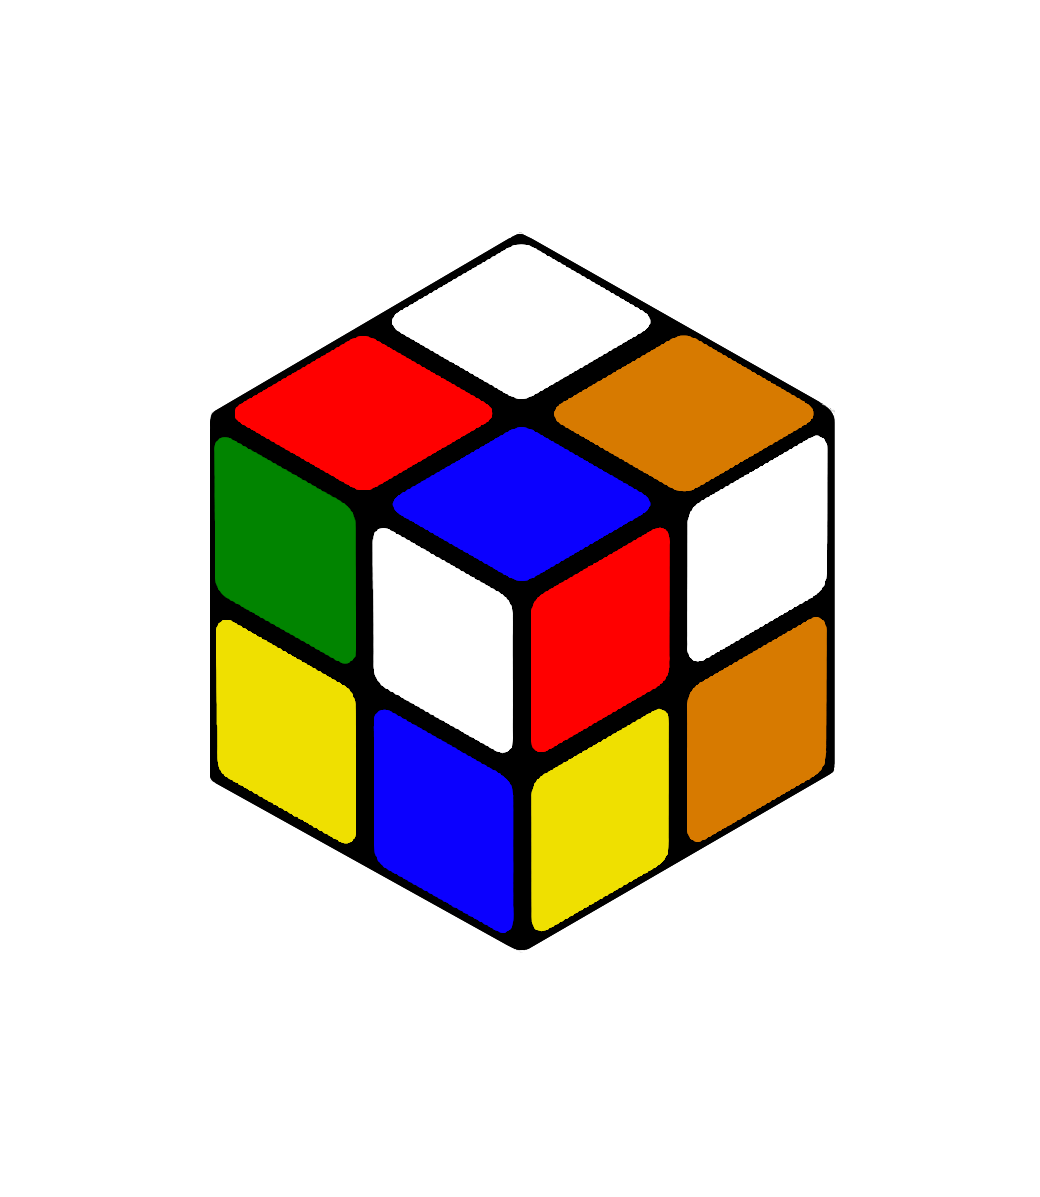
\includegraphics[scale=0.12]{LLFF_5.png}
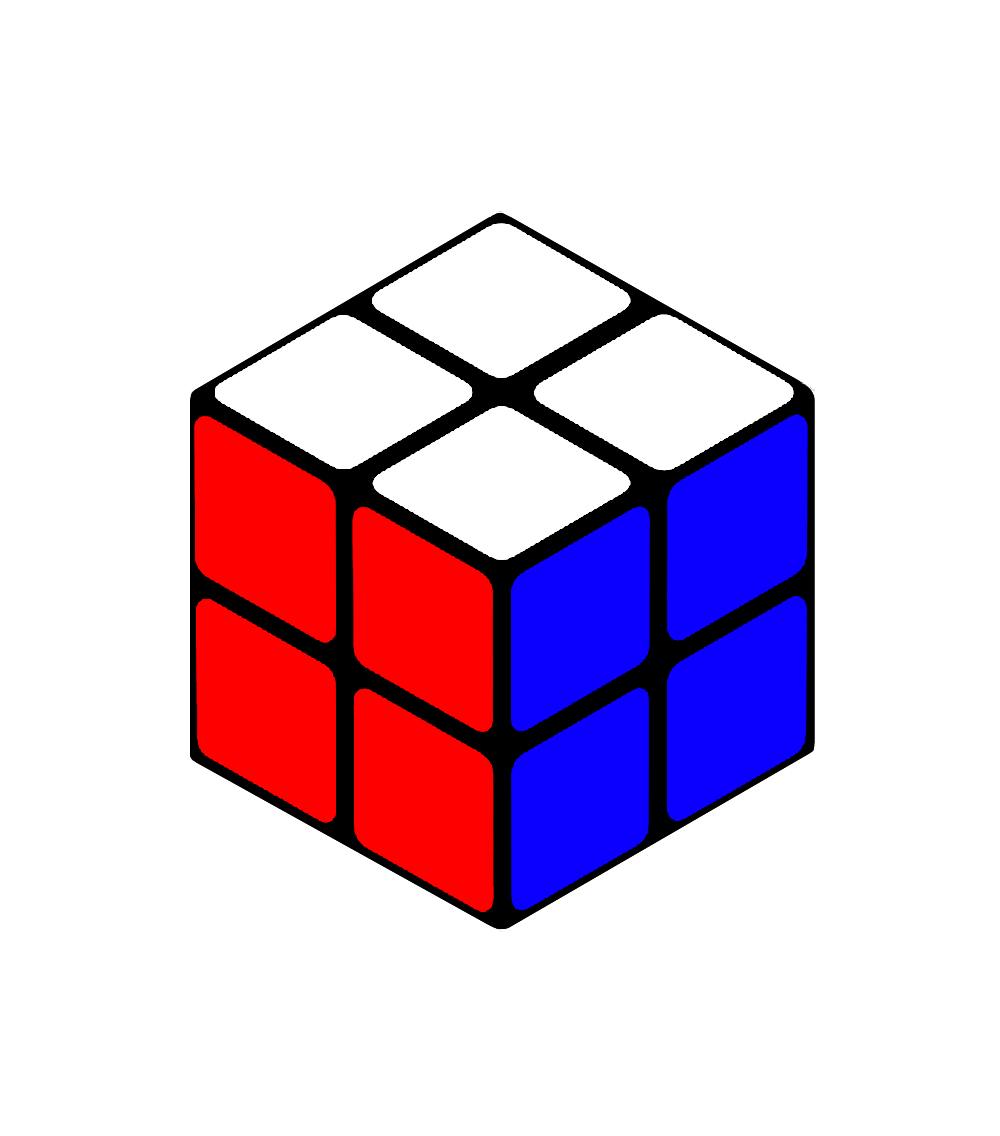
\includegraphics[scale=0.12]{2x2solved.png}
\caption{Ordnung des Zuges und der Permutation $LF$}
\label{Abbildung_LF_5_15}
\end{figure}

Links in Abbildung \ref{Abbildung_LF_5_15} ist zu sehen, dass alle Würfelsteine an der jeweiligen Ausgangsposition sind, aber nicht richtig ausgerichtet. Wird auf die Startkonfiguration $(1,0)$ der Zug $(LF)^5$ angewandt, gelangt man zu dieser Folgekonfiguration:
\begin{align*}
(1,0) \cdot (LF)^5 = (1, (1,0,1,1,1,0,1,1))
\end{align*}
Der Würfel ist nach fünf Wiederholungen von $LF$ nicht gelöst, da die Ausrichtung der Steine verändert ist -- der Vektor $x$ ist nicht 0. Die Ordnung der Permutation von $LF$ ist 5, da die Funktion $\sigma$ nach fünffachem Ausführen 1 ist. Die Ordnung des Zuges von $LF$ ist allerdings 15, da sich der Würfel erst dann wieder in seiner Ausgangskonfiguration befindet. Somit ist die Würfelkonfiguration nach dem Ausführen von $(LF)^{15}$ auf dem Startzustand wieder $(1,0)$:
\begin{align*}
(1,0) \cdot (LF)^{15} = (1,0)
\end{align*}
Das gilt dann auch für jede andere Startkonfiguration nach Ausführen des Zuges $(LF)^{15}$:
\begin{align*}
(\sigma, x) \cdot (LF)^{15} = (\sigma, x)
\end{align*}

\subsubsection*{Definition: Ordnung einer Permutation}

Die Ordnung einer Permutation ist im Folgenden mathematisch definiert. Dabei ist $(\sigma, x)$ eine beliebige Würfelkonfiguration.
\begin{align*}
\forall \ Z \in \Gtwo \ \exists \ n \in \mathbb{N} \ . \ (\sigma, x) \cdot Z^n = (\sigma, x')
\end{align*}
Demnach gibt es für jeden beliebigen Zug $Z$ eine natürliche Zahl $n$, die die Ordnung der Permutation des Zuges ist. Wird dieser Zug $Z$ $n$-mal ausgeführt, befindet sich die Permutationsfunktion $\sigma$ wieder im Ausgangszustand. Der Vektor $x$ wird dabei nicht berücksichtigt.




\subsubsection*{Zykelstruktur}



\label{Abschnitt_Zykelstruktur}

Die Ordnung einer Permutation lässt sich anhand ihrer Zykelstruktur bestimmen. Zu Beginn dieses Abschnitts wurde die Ordnung einer Permutation bereits definiert und beschrieben. Dabei handelt es sich um die Anzahl der Wiederholungen, die für einen Zug notwendig sind, damit die Steine die gleiche Anordnung wie zu Beginn des Zuges haben. Dabei geht es um die Steinpositionen und nicht um die Steinausrichtungen.

Beispielsweise besteht die Permutationsfunktion $\sigma_U =\ ( \ \textit{ulf} \ \textit{ulb} \ \textit{urb} \ \textit{urf} \ ) $  des Zuges $U$ (eine Drehung der oberen Ebene um $90^\circ$ im Uhrzeigersinn) aus genau einem vierelementigen Zykel.
Wird der Zug $U$ viermal ausgeführt, befinden sich die Würfelsteine wieder in ihrer vorherigen Position. In der folgenden Tabelle ist das vierfache Ausführen der Permutation $\sigma_U$ abgebildet.
\begin{center}
\begin{tabular}{ccccc}
\toprule
\textbf{Ausführung} & \textbf{ulf} & \textbf{ulb} & \textbf{urb} & \textbf{urf} \\
\midrule
1 & ulb & urb & urf & ulf \\

2 & urb & urf & ulf & ulb \\

3 & urf & ulf & ulb & urb \\

4 & ulf & ulb & urb & urf \\
\bottomrule
\end{tabular}
\end{center}

Die vierte Zeile der Tabelle hat dieselbe Anordnung der Steine wie die oberste Zeile (vor Ausführung von $U$). 
Somit hat die Permutation der beschriebenen Ebenenrotation $U$ die Ordnung 4, da $\sigma_U$ nach vier Wiederholungen wieder zur Ausgangspermutation führt. Das gilt auch für die anderen einelementigen Züge ($D, F, B, L, R$).
Bei jeder Permutation eines Zuges $Z$, die aus lediglich einem $n$-elementigen Zykel besteht, ist die Ordnung der Permutation $n$. Dabei ist $n$ eine natürliche Zahle $\mathbb{N}$ und $(\sigma, x)$ eine beliebige Würfelkonfiguration:
\begin{align*}
\forall \ Z \in \Gtwo \ \textit{mit} \ \sigma_Z=(i_1 \ i_2 \ ... \ i_n) \ . \  (\sigma, x) \cdot Z^n= (\sigma, x')
\end{align*}
Wenn der Zug $Z$ mehrfach ausgeführt wird, wird nach jeder $n$-ten Wiederholung der Ausgangszustand der Permutationen erreicht. \cite{TD} 
Es gilt folglich auch:
\begin{align*}
\forall \ Z \in \Gtwo \ \textit{mit} \ Z=(i_1 \ i_2 \ ... \ i_n), \ n,k \in \mathbb{N} \ . \  {(\sigma, x) \cdot Z^{k*n}=(\sigma, x') }
\end{align*}
Auch bei komplexeren Permutationen von Zügen, die aus mehr als einem Zykel bestehen, kann anhand der Zykelstruktur die Ordnung bestimmt werden. Dazu muss das \textit{kleinste gemeinsame Vielfache} aller Zykelgrößen bestimmt werden. \cite{TD}

 
Der besseren Übersichtlichkeit halber sind die Zykel aller Züge in Abbildung \ref{Abbildung_GraphAllerPermutationen} grafisch dargestellt.
Dieser Graph vereinfacht das Ablesen der Zykel, wenn bei einem Zug mehrere Ebenenrotationen kombiniert werden.
\begin{figure}[H]
\centering
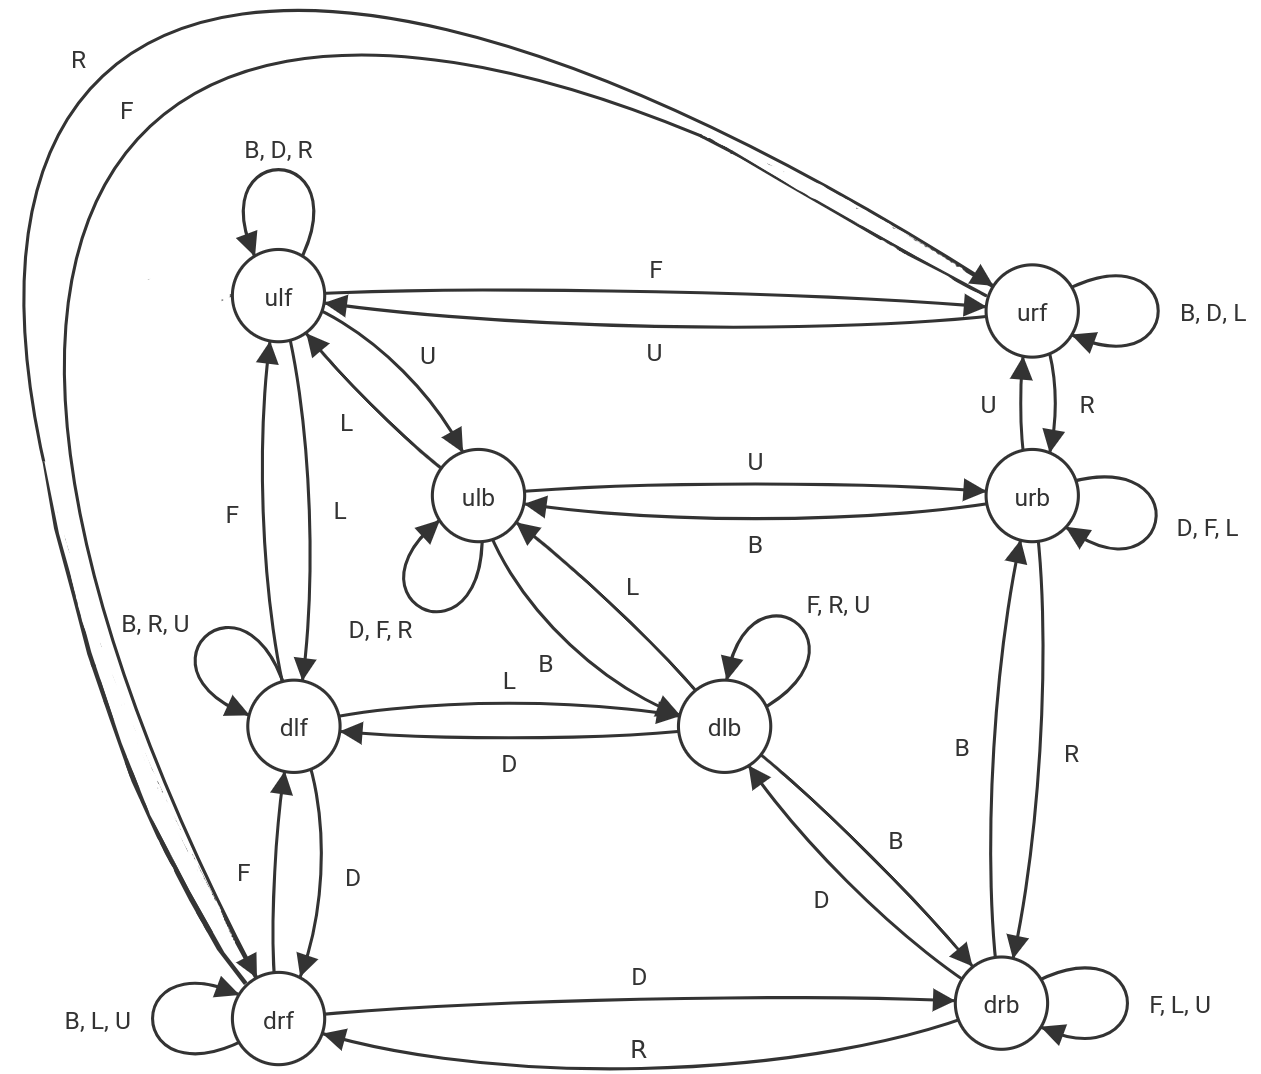
\includegraphics[scale=0.25]{graph_zug1.png}
\caption[Graph aller Zugpermutationen]{Graph aller Zugpermutationen}
\label{Abbildung_GraphAllerPermutationen}
\end{figure}

Mithilfe des Graphen oder der Permutationsfunktionen $\sigma$ kann nun die Zykelstruktur der Permutationen für den Beispielzug $LLFF$ dargestellt werden. 
Dazu wird eine Tabelle erstellt, die zeilenweise jede Position auf ihre neue Position abbildet. Der Zug $LLFF$ setzt sich aus den Zügen $L$ und $F$ zusammen. 

\begin{center}
\begin{tabular}{ccccccccc}
\toprule
\textbf{Zug} & \textbf{ulb} & \textbf{urb} & \textbf{ulf} & \textbf{urf} & \textbf{dlb} & \textbf{drb} & \textbf{dlf} & \textbf{drf} \\
\midrule

L & ulf & \textcolor{gray}{urb} & dlf & \textcolor{gray}{urf} & ulb & \textcolor{gray}{drb} & dlb & \textcolor{gray}{drf} \\

L & dlf & \textcolor{gray}{urb} & dlb & \textcolor{gray}{urf} & ulf & \textcolor{gray}{drb} & ulb & \textcolor{gray}{drf} \\

F & ulf & \textcolor{gray}{urb} & \textcolor{gray}{dlb} & drf & urf & \textcolor{gray}{drb} & \textcolor{gray}{ulb} & dlf \\

F & urf & \textcolor{gray}{urb} & \textcolor{gray}{dlb} & dlf & drf & \textcolor{gray}{drb} & \textcolor{gray}{ulb} & ulf \\
\bottomrule
\end{tabular}
\end{center}

Die grauen Einträge bleiben bei der jeweiligen Ebenenrotation unverändert. 
Die Zykel des Zuges $LLFF$ sind in Abbildung \ref{Abbildung_ZykelVonLLFF} grafisch dargestellt. Dort ist zu sehen, dass $LLFF$ aus zwei einelementigen und zwei dreielementigen Zykeln besteht.
\begin{figure}[H]
\centering
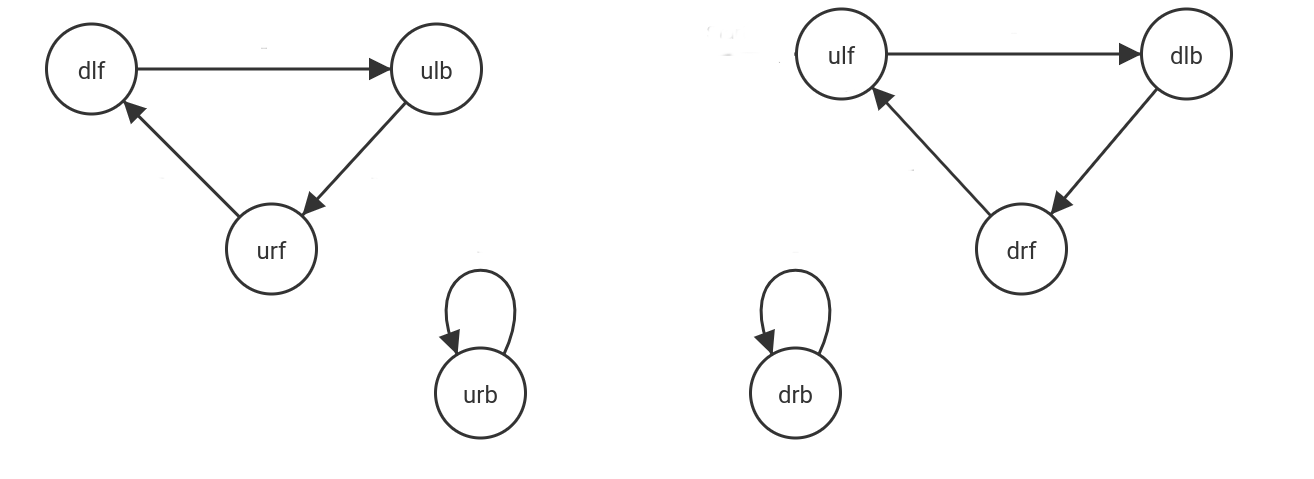
\includegraphics[scale=0.25]{zykel_LLFF.png}
\caption[Zykel des Zuges $LLFF$]{Zykel des Zuges $LLFF$}
\label{Abbildung_ZykelVonLLFF}
\end{figure}
In der Zykelschreibweise wird der Zug $LLFF$ somit als $\sigma_{LLFF}=( \ \textit{dlf} \ \textit{ulb} \ \textit{urf}\ )(\ \textit{ulf} \ \textit{dlb} \ \textit{drf} \ )$ geschrieben.
Da es zwei Zykel der Länge drei gibt, befinden sich alle Würfelsteine nach drei Zügen wieder in ihrer Ausgangsposition:
\begin{align*}
kgV(3,3,1,1)=3
\end{align*}
Die Permutation des Zuges $LLFF$ hat also die Ordnung $3$.


Außerdem kann abgelesen werden, dass sechs der acht Steine bei dem Zug $LLFF$ bewegt werden. Die anderen beiden (\textit{urb} und \textit{drb}) bleiben unverändert. Das kann beispielsweise an der grafischen Abbildung der Zykel (\ref{Abbildung_ZykelVonLLFF}) gesehen werden.


Bei dem Beispielzug $LLFF$ ist nach dreifacher Ausführung des Zuges nicht ausschließlich die Position der Steine korrekt sondern auch die Ausrichtung. Somit ist die \textit{Ordnung des Zuges} auch 3. Darauf wird genauer in Abschnitt \ref{Abschnitt_OrdnungZüge} eingegangen.

\subsubsection*{Algorithmus}

Aus diesen Erkenntnissen ergibt sich folgender Algorithmus zur Bestimmung der Ordnung einer Permutation. Als Eingabeparameter wird ein Zug $Z$ übergeben. Die Rückgabe ist die Permutationsordnung des Zuges $Z$.

\begin{minipage}[H]{0.14\textwidth}
      $\ $
\end{minipage}
\begin{minipage}[H]{0.72\textwidth}
\begin{algorithm}[H]
\LinesNumbered
\DontPrintSemicolon
\SetNlSty{textbf}{}{\ }
\SetAlgoNlRelativeSize{0}
\KwData{Zug $Z$}
\KwResult{\textit{kgVList} ist die Ordnung der Permutation}
\BlankLine
 \textit{perm} $\leftarrow$ Permutationsfunktion von Zug $Z$\;

  \textit{list} $\leftarrow$ leere Liste initialisieren\;

  \textit{z} $\leftarrow$ Anzahl der Zykel von $perm$ \; 

 \While{\textit{z} $>$ \textit{0}}{
 
  \textit{zykel\_length} $\leftarrow$ Zykellänge von Zykel $z$ \;
  
  \textit{list} $\leftarrow$ \textit{zykel\_length} hinzufügen \;
  
  \textit{z} $\leftarrow$ \textit{ z}$-1$ \;
 }
  \textit{kgVList} $\leftarrow$ \textit{kgV} von Elementen aus \textit{list} berechnen \;

 return \textit{kgVList} \;

\caption{Ordnung einer Permutation bestimmen} 
\label{Algorithmus_OrdnungPermutation}
\end{algorithm}
\end{minipage}
\begin{minipage}[H]{0.14\textwidth}
      $\ $
\end{minipage}

\vspace*{1em}

In Zeile 1 wird die Permutationsfunktion des Zuges der Variablen \textit{perm} zugewiesen und in Zeile 2 wird eine leere Liste initialisiert, um darin die Längen der einzelnen Zykel zu speichern. Danach wird in Zeile 3 die Anzahl der Zykel ausgelesen und in der Variablen $z$ gespeichert. Daraufhin wird eine \textit{while}-Schleife $z$-mal ausgeführt. In jedem Durchlauf wird die Länge von einem der $z$ Zykel ausgelesen und in die Liste hinzugefügt. Außerdem wird $z$ dekrementiert. Nachdem alle Zykellängen in \textit{list} gespeichert sind, wird in Zeile 8 das \textit{kleinste gemeinsame Vielfache} der Listenelemente berechnet und der Variablen \textit{kgVList} zugewiesen. Dabei handelt es sich um die Ordnung der Permutation und deshalb wird \textit{kgVList} in Zeile 9 zurückgegeben.

Die Ordnung der Permutation wird zur Berechnung der Ordnung von Zügen benötigt. Diese wird im folgenden Abschnitt beschrieben und es wird ein Algorithmus zur Berechnung eingeführt.

%
%
%
%
%
%
%
%=======================================================================================================
%
%
%
%
%

\subsection{Ordnung der Züge}
\label{Abschnitt_OrdnungZüge}

In diesem Abschnitt wird gezeigt, dass der Würfel wieder in die Ausgangsposition gelangt, wenn ein beliebiger Zug $Z \in \Gtwo$ wiederholt auf den Würfel angewendet wird. Das wird in der folgenden Formel dargestellt, dabei ist $C$ eine beliebige Würfelkonfiguration.
\begin{align*}
\forall \ Z \in \Gtwo \ \exists \ n \in \mathbb{N} \ . \ C \cdot Z^n = C
\end{align*}
Außerdem wird ein Algorithmus zu Berechnung der Ordnung von Zügen beschrieben.

\subsubsection*{Beweis}

Der folgende Beweis orientiert sich an dem Beweis aus \textit{Group Theory via Rubik's Cube} von Tom Davis \cite{TD}.

Jedes Mal wenn ein Zug wiederholt wird, werden die Steine im Würfel neu angeordnet und ausgerichtet. 
Da es eine endliche Anzahl an Würfelkonfigurationen gibt, muss eine Würfelkonfiguration wiederholt werden, wenn ein Zug oft genug durchführt wird.
Die Zahl der validen Würfelkonfigurationen ist zwar sehr groß, aber endlich ($3 \, 674 \, 160$). Demnach muss eine Konfiguration wiederholt werden, wenn der Zug häufiger ausgeführt, als es mögliche Würfelkonfigurationen gibt. Die Anzahl der validen Würfelkonfigurationen wird in Kapitel \ref{Kapitel_ValideKonfigurationen} berechnet.

Übertragen auf das mathematische Modell des Würfels bedeutet das folgendes: Bei einem beliebigen Zug $Z \in \Gtwo$, der auf eine Konfiguration $C$ angewandt wird, wird nach wiederholtem Ausführen eine Würfelkonfiguration wiederholt. Wenn die wiederholte Konfiguration $C'$ zuerst nach $n \in \mathbb{N}$ Wiederholungen des Zuges $Z$ auftritt und das zweite Mal nach $m \in \mathbb{N}$ Wiederholungen, gilt: 
\begin{align*}
C' = C \cdot Z^n& = C \cdot Z^m \textit{ mit } 0<n<m 
\end{align*}
Da $n$ und $m$ das erste Vorkommen einer wiederholenden Konfiguration repräsentieren, gilt dann auch:
\begin{align*}
C \cdot Z^{n-1} \neq C \cdot Z^{m-1}
\end{align*}

Wenn auf die gleiche Ausgangskonfiguration $C$ $n$-mal oder $m$-mal der Zug $Z$ angewandt wird, erreicht man die gleiche Folgekonfiguration $C'$.
Wird auf diese Folgekonfiguration $C'$ dann der Zug $Z^{-1}$ angewandt, ist die Folgekonfiguration $C'''$ wieder gleich. Dabei ist es irrelevant, ob vorher $n$-mal oder $m$-mal $Z$ ausgeführt wurde. Von der gleichen Ausgangskonfiguration ausgehend wird die gleiche Folgekonfiguration erreicht, wenn der gleiche Zug ausgeführt wird. Demnach gilt:
\begin{alignat*}{2}
\ &(C \cdot Z^n) \cdot Z^{-1} && = (C \cdot Z^m) \cdot Z^{-1}  \\
\Leftrightarrow \ & C' \cdot Z^{-1} && = C' \cdot Z^{-1} \\
\Leftrightarrow \ & C'' && = C ''
\end{alignat*}


Beim Anwenden von $Z^{-1}$ auf die Konfiguration $C'$ wird die letzte Ausführung von $Z$ wieder rückgängig gemacht, da $Z^{-1}$ das Inverse des Zuges $Z$ ist. Wenn der Zug $Z$ $n$-mal ausgeführt wird und danach $Z^{-1}$ ausgeführt wird, ist es das gleiche wie $n-1$-mal $Z$ auszuführen. Folglich gilt:
\begin{align*} 
(C \cdot Z^n) \cdot Z^{-1}=C \cdot (Z^n \circ Z^{-1})=C \cdot Z^{n-1}
\end{align*}
Demnach gilt dann :
\begin{alignat*}{2}
 & (C \cdot Z^n) \cdot Z^{-1} && = (C \cdot Z^m) \cdot Z^{-1}  \\
\Leftrightarrow \ &  C \cdot Z^{n-1} && = C \cdot Z^{m-1}
\end{alignat*}
Das widerspricht dann aber der Annahme, dass $m$ der kleinste Wert für eine Wiederholung der Konfiguration ist. In diesem Fall ist $n-1$ bzw. $m-1$ die kleinste Anzahl an Ausführungen für eine wiederholende Konfiguration:
\begin{alignat*}{2}
 & (C \cdot Z^n) \cdot Z^{-1} && = (C \cdot Z^m) \cdot Z^{-1} \\
\Leftrightarrow \ & C \cdot Z^{n-1} && = C \cdot Z^{m-1} \\
\Leftrightarrow \ & C'' && = C''
\end{alignat*}
Deshalb muss $n=0$ sein, damit $m$ die erste Wiederholung einer Position repräsentiert. 

Daraus folgt: Wenn ein Zug wiederholt auf einen Würfel angewendet wird, kommen die Steine wieder in die Ausgangsposition.

\subsubsection*{Algorithmus}

Es wurde bereits gezeigt, dass sich eine Würfelkonfiguration wiederholt, wenn ein beliebiger Zug wiederholt angewandt wird. Die Anzahl der Wiederholungen eine Zuges, bis der Würfel wieder in der Ausgangskonfiguration ist, nennt man Ordnung eines Zuges. Für die Berechung dieser wird nun ein Algorithmus entworfen, der als Pseudocode dargestellt wird. Dazu wird der Algorithmus \ref{Algorithmus_OrdnungPermutation} zur Berechnung der Ordnung einer Permutation benötigt.

Der Algorithmus braucht für die Berechung der Ordnung eines Zuges $Z$ zwei Eingabeparameter: Den Zug $Z$ und die Ausgangskonfiguration $C$ des Würfels. Die Ausgabe ist die Ordnung eines Zuges.


\begin{minipage}[H]{0.15\textwidth}
      $\ $
\end{minipage}
\begin{minipage}[H]{0.65\textwidth}
\begin{algorithm}[H]
\LinesNumbered
\DontPrintSemicolon
\SetNlSty{textbf}{}{\ }
\SetAlgoNlRelativeSize{0}
\KwData{Konfiguration $C(\sigma, x)$, Zug $Z$}
\KwResult{\textit{kgV(count, ord)} ist Ordnung eines Zuges}

 \textit{ord} $\leftarrow$ Ordnung der Permutation von $Z$\;
  \textit{x'} $\leftarrow$ \textit{x}\;
  \textit{count} $\leftarrow$ 1\;

  $C \leftarrow C \cdot  Z^\textit{ord}$ \; 
 \While{\textit{x} $\neq$ \textit{x'}}{
  $C \leftarrow C \cdot Z^\textit{ord}$\;
   \textit{count} $\leftarrow$ \textit{count} + 1 \;
 }
 return \textit{kgV(count, ord)} \;

\caption{Ordnung eines Zuges bestimmen} 
\label{Algorithmus_OrdnungZug}
\end{algorithm}
\end{minipage}
\begin{minipage}[H]{0.2\textwidth}
      $\ $
\end{minipage}

\vspace*{1em}

In Zeile 1 wird die Variable \textit{ord} mit der Ordnung der Permutationen von $Z$ intialisiert. Die Berechnung der Permutationsordnung wurde in Abschnitt \ref{Abschnitt_Zykelstruktur} in Algorithmus \ref{Algorithmus_OrdnungPermutation} beschrieben. Dann wird der Startwert des Vektors \textit{x} in der Variablen \textit{x'} gespeichert, um in der weiteren Berechnung Vergleiche damit durchzuführen (Zeile 2). Außerdem wird in Zeile 3 die Variable \textit{Count} mit 1 initialisiert -- sie zählt die nötigen Ausführungen des Zuges $Z$, bis der Vektor wieder in der Ausgangskonfiguration ist. \textit{count} wird mit 1 initialisiert, da vor der \textit{while}-Schleife in Zeile 4 bereits eine Anwendung von $Z$ durchgeführt wird. Die Anzahl der Ausführung von $Z$ ist dabei immer \textit{ord}, da die Ordnung des Zuges die Ausrichtung der Steine und die Steinposition berücksichtigt. Die Steine sind ausschließlich nach Vielfachen von \textit{ord} Zügen an der richtigen Position.

Die \textit{while}-Schleife in Zeile 5 wird ausgeführt, bis \textit{x} wieder in der gleichen Konfiguration wie zum Start ist. Bei jeder Ausführung wird $Z^\textit{ord}$ ausgeführt (Zeile 6) und \textit{count} inkrementiert (Zeile 7).
Die Ordnung des Zuges $Z$ setzt sich zusammen aus der Ordnung der Permutation von $Z$ und der Anzahl der Durchführungen von $Z^\textit{ord}$, bis die Ausrichtung der Steine wieder in der Anfangskonfiguration ist. Daher ist die Ordnung eines Zuges das \textit{kleinste gemeinsame Vielfache} von diesen beiden Werten (Zeile 8).



%
%
%
%
%
%
%
%
%
%
%=======================================================================================================
%
%
%
%
%
%
%
%
%
%
%\subsection*{Äquivalenz von Zügen}\addcontentsline{toc}{subsection}{\protect\numberline{}Äquivalenz von Zügen}


%Es kann schwierig sein, die Äquivalenz von Zügen oder Roatationen anhand der Funktionen ($\sigma$ und $\delta$) in der Zykelschreibweise zu erkennen. 
%Das liegt daran, dass die Zykel in verschiedener Reihenfolge geschrieben werden können. So ist der Zug $U$ beispielsweise $ ( \ \textit{ulf} \ \textit{ulb} \ \textit{urb} \ \textit{urf} \ )$, aber auch $( \ \textit{urb} \ \textit{urf} \ \textit{ulf} \ \textit{ulb} \ )$.
%Um das zu vereinfachen, werden die Würfelpositionen priorisiert, so dass die Position mit der höchsten Priorität immer vorne steht und zwei Äquivalente Zykel somit gleich aussehen. 
%Die Positionen werden wie folgt priorisiert:
%\begin{center}
%\begin{tabular}{lcccccccc}
%Priorität & 1 & 2 & 3 & 4 & 5 & 6 & 7 & 8 \\
%\hline
%Position  & ulb & urb & ulf & urf & dlb & drb & dlf & drf \\
%\end{tabular}
%\end{center}
%Somit ist die angepasste Schreibweise für den Zug $U$ dann $( \ \textit{ulb} \ \textit{urb} \ \textit{urf} \ \textit{ulf} \ )$, da \textit{ulb} (falls vorhanden) ganz vorne stehen muss.

%
%
%
%
%
%
%
%
%
%
%=======================================================================================================
%
%
%
%
%
%
%
%
%
%
\newpage

\section{Untergruppen von G$_{2\times 2\times 2}$}

\label{Kapitel_Untergruppen}

Dieses Kapitel behandelt einige der Untergruppen der Gruppe $(\Gtwo, \circ)$. Im ersten Teil wird auf die trivialen Untergruppen eingegangen, außerdem werden noch weitere Untergruppen beschrieben.
Die Definition und Erklärung der Untergruppe und des Erzeugers findet sich in Abschnitt \ref{Abschnitt_Untergruppe}.
Außerdem werden die Cayleygraphen zu zwei Untergruppen dargestellt und erklärt. Die Cayleygraphen dienen der Veranschaulichung von Gruppenstrukturen. Die Untergruppe, die den \Ttwo Würfel minimal aber komplett abbildet, findet sich in Kapitel \ref{Kapitel_MinUntergruppe}.

%
%
%
%
%
%
%
%
%
%
%=======================================================================================================
%
%
%
%
%
%
%
%
%
%
\subsection{Beispiel-Untergruppen}

\label{Abschnitt_UntergruppenBeispiele}

Wie bereits in Abschnitt \ref{Abschnitt_Untergruppe} erklärt, hat jede Gruppe zwei triviale Untergruppen. Die beiden trvialen Untergruppen von $(\Gtwo, \circ)$ werden hier $(H_N, \circ)$ und $(H_G, \circ)$ genannt: 
\begin{align*}
(H_N, \circ) \leqslant (\Gtwo, \circ)\textit{ und }(H_G, \circ) \leqslant (\Gtwo, \circ)
\end{align*} 
Die Untergruppe $(H_N, \circ)$ enthält in der Trägermenge $H_N$ ausschließlich die Äquivalenzklasse des neutralen Elements $N$. Bei der Untergruppe $(H_G, \circ)$ hingegen ist die Trägermenge $H_G$ die gleiche Menge wie $\Gtwo$. 
\begin{align*}
(H_N, \circ) = (\{N\}, \circ)\textit{ und }  (H_G, \circ) = (\Gtwo, \circ)
\end{align*}
Im Rahmen dieser Arbeit kann nur auf einen Teil der Unterguppen von $(\Gtwo, \circ)$ eingegangen werden. 
Der folgende Abschnitt beschreibt zwei anschauliche Untergruppen des Würfels. Diese Untergruppen hat Tom Davis (in  \textit{Group Theory via Rubik's Cube}) \cite{TD} für den 3x3x3-Würfel genannt. Hier werden zwei seiner Untergruppen auf den 2x2x2 übertragen: 
\begin{itemize}
\item Die Untergruppe $(H_{E1}, \circ)$ lässt nur die Rotation einer Ebene zu. Die Züge der Trägermenge erreichen lediglich vier Würfelkonfigurationen (sowohl beim 2x2x2- als auch beim 3x3x3-Würfel). Das kann auch gut an einem \textit{Cube} nachvollzogen werden, da durch das Drehen von nur einer Ebene auch nur vier verschiedene Ergebnisse erzielt werden können.

Da die Trägermenge $H_{E1}$ die Äquivalenzklassen aller möglichen Züge der Untergruppe beinhaltet, sind hier genau vier Elemente enthalten. Jeder Zug, der durch die Drehung einer Ebene ausgeführt wird, ist ein Repräsentant dieser vier Züge.

Auch anhand des mathematischen Modells des \Ttwo Würfels kann festgestellt werden, dass die Züge der Untergruppe $(H_{E1}, \circ)$ genau vier Würfelkonfigurationen erreichen.

Jede Ebenendrehung ($U, D, R, L, F$ oder $B$) ist durch eine Permutationsfunktion $\sigma$ definiert. Dabei besteht $\sigma$ für jeden dieser Grundzüge aus nur einem vierelementigen Zykel. Diese Zykel wurden in Abschnitt \ref{Abschnitt_PositionenDerSteineImWürfel} definiert. Die Ordnung der Permutation ist im Fall einer einzelnen Ebenendrehung immer vier. Die Ordnung einer Permutation wurde in Abschnitt \ref{Abschnitt_OrdnungPermutationen} beschrieben.

Die Ordnung eines Zuges wurde in Abschnitt \ref{Abschnitt_OrdnungZüge} definiert. Bei der Ordnung eines Zuges wird zusätzlich zu den Permutationen die Funktion $\gamma$ berücksichtig, die die Ausrichtung der Steine darstellt. $\gamma$ wurde in Abschnitt \ref{Abschnitt_AusrichtungDerSteine} definiert. Jede dieser Funktionen $\gamma$ gibt die Eingabe unverändert zurück, wenn sie viermal direkt nacheinander ausgeführt wird. Der Beweis dazu findet sich in Anhang \ref{Anhang_Ausrichtungsfunktionen}. 

Somit ist die Ordnung einer einzelnen Ebenendrehung immer vier und die Trägermenge $H_{E1}$ enthält genau vier Züge. Durch diese vier Züge können genau vier verschiedene Würfelkonfigurationen erreicht werden. 



\item Eine weitere Untergruppe von $(\Gtwo, \circ)$ ist $(H_{E2}, \circ)$. Hier dürfen zwei gegenüber\-liegende Ebenen gedreht werden. 
Bei der Gruppe des \Tthree Würfels ergeben sich daraus 16 mögliche Würfelkonfigurationen \cite{TD}. Bei dem \Ttwo \textit{Cube} sind es allerdings lediglich vier, da es nur zwei Ebenen gibt und die Rotation der Würfels nicht anhand der Mittelsteine unterschieden werden kann. Durch die Äquivalenzklassen der Rotationen ergibt sich somit eine zu $(H_{E1}, \circ)$ äquivalente Untergruppe.
\end{itemize}


%
%
%
%
%
%
%
%
%
%
%=======================================================================================================
%
%
%
%
%
%
%
%
%
%

\subsection{Erzeuger}
\label{Abschnitt_ErzeugerGF}

Die folgenden Beispiele stammen aus Tom Davis' \textit{Group Theory via Rubik's Cube} \cite{TD} und werden hier von der Gruppe des \Tthree \textit{Cubes} auf den \Ttwo \textit{Cube} übertragen. Erzeuger wurden in Abschnitt \ref{Abschnitt_Erzeuger} definiert und erklärt.


Ein Beispiel für einen Erzeuger einer Untergruppe $(G_F, \circ)$ von $(\Gtwo, \circ)$ ist der einzelne Zug $\{ F \}$, der diese Untergruppe erzeugt. Durch den Zug $F$ können genau vier Würfelkonfigurationen erreicht werden und die Trägermenge $G_F$ der Untergruppe $(G_F, \circ)$ enthält somit vier Elemente:
\begin{align*}
G_F = \{N, F, FF, FFF\}
\end{align*}
Alle weiteren Züge, die durch $F$ erzeugt werden, sind äquivalent zu einem dieser Züge sind. Beispielsweise ist $FFFF$ ein Repräsentant der Äquivalenzklasse von $N$ -- der Würfel befindet sich nach Ausführen dieses Zuges wieder in der Ausgangsposition.


Ein weiteres Beispiel ist die Untergruppe, die von $\{FF\}$ erzeugt wird. Dabei kann die obere Ebene ausschließlich halbe Drehungen (statt Vierteldrehungen) machen und somit nur zwei Positionen erreichen. Die Trägermenge enthält daher die Äquivalenzklassen der beiden Züge $FF$ und $FFFF$.


Die komplette Gruppe $(\Gtwo, \circ)$ wird erzeugt durch $\{U, D, R, L, F, B\}$. Eine minimale Gruppe des \Ttwo Würfels wird in Kapitel \ref{Kapitel_MinUntergruppe} beschrieben und durch $\{U, R, F\}$ erzeugt.

Die Untergruppen, die von genau einem Element aus $\Gtwo$ erzeugt werden, nennt man zyklische Gruppen. Die oben beschriebene Untergruppe $(G_F, \circ)$, die durch $ F $ erzeugt wird, ist eine solche zyklische Untergruppe.
$(G_F, \circ)$ wird erzeugt durch:
\begin{align*}
\langle F \rangle = \{ F^n \mid n \in \mathbb{Z}\}
\end{align*}
Das bedeutet, dass die Trägermenge $G_F$ die Äquivalenzklassen der folgenden Elemente enthält: 
\begin{align*}
\{N, F^1, F^2, F^3, F^4, ...\}
\end{align*}
Zyklische Gruppen können unendlich sein. Die Gruppe $(G_F,  \circ)$ ist aufgrund der Äquivalenzklassen aber endlich. Die Gleichheit der einelementigen Züge wurde bereits in Abschnitt \ref{Abschnitt_GleichheitVonZügen} beschrieben.


Da die Gruppe $(\Gtwo, \circ)$ endlich ist, erzeugt jedes Element der Gruppe eine endliche zyklische Untergruppe \cite{TD}. Die Größe dieser Untergruppe hängt von der Ordnung des Zuges ab. Die Ordnung wurde in Abschnitt \ref{Abschnitt_OrdnungPermutationen} beschrieben.
Die Ordnung des Zuges $FR$ beispielsweise ist 15 -- wenn $FR$ 15-mal auf dem \Ttwo Würfel ausführt wird, ist er wieder in der Ausgangsposition. 
Die Gruppe, die durch $\{FR\}$ erzeugt wird, hat somit 15 Elemente, da mit dem Zug 15 Würfelkonfigurationen erreichbar sind. Bei dem \Tthree Würfel ist die Ordnung des Zuges $FR$ 105 \cite{TD}.
%
%
%
%
%
%
%
%
%
%=======================================================================================================
%
%
%
%
%
%
%
%
%
%

\subsection{Durch \textit{FF} und \textit{RR} erzeugte Untergruppe}
\label{Abschnitt_UntergruppeFFRR}

Das Beispiel der durch $\{ FF, RR \}$ erzeugten Untergruppe hat Tom Davis in \textit{Group Theory via Rubik's Cube} \cite{TD} ebenfalls beschrieben und hier wird es von dem \Tthree \ auf den \Ttwo Würfel übertragen.
Da die beiden Züge $FF$ und $RR$ als Einheiten gesehen werden, muss jede der Ebenendrehungen eine halbe Drehung sein.
Es wurde in Abschnitt \ref{Abschnitt_GleichheitVonZügen} bereits gezeigt, dass $(FF)^2 = N$ und $(RR)^2$ Repräsentanten der Äquivalenzklasse von $N$ sind, da der Würfel dann wieder in der Ausgangskonfiguration ist.
\begin{align*}
C \cdot (FF)^2 = C \textit{ und } C \cdot (RR)^2 = C
\end{align*}

Wenn bei einem gelösten \Ttwo Würfel $FFRR$ ausgeführt wird, befindet sich der Würfel nach 3 Wiederholungen wieder in der Startkonfiguration. Das gilt auch für den Zug $RRFF$. Die Ordnung von $FFRR$ und $RRFF$ ist daher 3. Bei dem \Tthree \textit{Cube} ist die Ordnung dieser Züge 6 \cite{TD}.
Die durch $\{ FF, RR \}$ erzeugte Untergruppe des \Tthree Würfels hat somit mehr Elemente als die des \Ttwo Würfels. 

Im Folgenden werden alle Mitglieder der Untergruppe des \Ttwo \textit{Cubes} aufgelistet. Alle anderen möglichen Kombinationen von $FF$ und $RR$ erreichen dieselbe Würfelkonfiguration wie diese sieben Züge:
\begin{center}
\centering
\begin{tabular}{c c c c}
$N$ & $RR$ & $FFRR$ &  $RRFFRR$ \\
& $FF$ & $RRFF$ & $FFRRFF$   \\
\end{tabular}
\end{center}
Zum Vergleich: Tom Davis erhält bei dem  \Tthree Würfel zwölf Elemente in der durch $\{ FF, RR \}$ erzeugten Untergruppe.
%, wenn dabei berücksichtigt wird, dass $FFFF$ und $RRRR$ keine Veränderung ergeben: $N$, $FF$, $RR$, $FFRR$, $RRFF$, $FFRRFF$, $FFRRFF$, $(FFRR)^2$, $(RRFF)^2$, $FF(RRFF)^2$, $RR(FFRR)^2$, $(FFRR)^2FF$ und $(RRFF)^2RR$. Da $FF$ und $RR$ die Ordnung 2 haben und $FFRR$ die Ordnung 3, sind alle komplexeren Zugkonkatenationen bereits abgedeckt.
%Wenn diese Züge an einem Würfel ausprobiert werden, stellt sich aber heraus, dass beispielsweise $(RRFF)^2RR$ bei gleichem Startzustand die gleiche Würfelkonfiguration wie $FF$ ergibt. 
%Wenn diese Doppelungen aussortiert werden, verbleiben folgende sieben Gruppenelemente:

Die äquivalenten Züge können auch mathematisch erkannt werden, ohne die Züge an einem Würfel auszuprobieren.
Das wird im Folgenden beispielhaft mit dem Zug $(RRFF)^2 RR$ gemacht.
\begin{align*}
(RRFF)^2 RR = RRFFRRFFRR
\end{align*}
Da $RRFF$ die Ordnung 3 hat, befindet sich der Würfel nach $(RRFF)^3$ wieder in der Ausgangskonfiguration.
\begin{align*}
C \cdot (RRFF)^3 = C \cdot RRFFRRFFRRFF = C
\end{align*}
Daraus kann geschlossen werden, dass nach dem Ausführen von $RRFFRRFFRR$ einzig $FF$ ausgeführt werden muss, um wieder in die Ausgangsposition zu gelangen. Somit kann die Position, die durch $RRFFRRFFRR$ erreicht wird, auch durch $(FF)^{-1}$ erreicht werden.
\begin{align*}
C \cdot RRFFRRFFRR = C \cdot (FF)^{-1}
\end{align*}
Da das Inverse eines Zuges $Z$ als $ZZZ$ definiert ist, gilt für die Züge $FF$ und $RR$:
\begin{align*}
(FF)^{-1} = F^{-1}F^{-1} = FFFFFF = FF \\
(RR)^{-1} = R^{-1}R^{-1} = RRRRRR = RR
\end{align*}
Die Inversen von $FF$ und $RR$ sind demnach $FF$ und $RR$. Deshalb ist der Zug $RRFFRRFFRR$ äquivalent zu dem Zug $FF$, da dieser äquivalent zu $(FF)^{-1}$ ist.
\begin{align*}
C \cdot RRFFRRFFRR = C \cdot FF
\end{align*}

Die Tatsache, dass $\{ FF, RR \}$ eine Untergruppen mit lediglich 7 bzw. 12 Elementen bei dem \Ttwo \  bzw. dem \Tthree Würfel erzeugt, ist besonders überraschend, da $\{ F, R \}$ bei dem  \Tthree Würfel eine Untergruppe der Größe $73\, 483\, 200$ erzeugt \cite{TD}. 
Bei dem \Ttwo \textit{Cube} kommt die Untergruppe mit $5! \cdot 3^5$ auf lediglich $29 \, 160$ Mitglieder, aber auch das ist deutlich größer als $7$.

%
%
%
%
%
%
%
%=======================================================================================================
%
%
%
%
%
%
%
%
%

\subsection{Cayleygraph}

Cayleygraphen wurden in Abschnitt \ref{Abschnitt_Cayleygraph} eingeführt. Sie dienen der Visualisierung von Untergruppen und deren Erzeugern.
Ein simples Beispiel ist in Abbildung \ref{Abbildung_CayleygraphF} zu sehen: Der Cayleygraph der Untergruppe $(G_F, \circ)$ von $(\Gtwo, \circ)$, die durch $\{ F \}$  erzeugt wird. Die Untergruppe $(G_F, \circ)$ wurde in Kapitel \ref{Abschnitt_ErzeugerGF} beschrieben.

\begin{figure}[H]
\centering
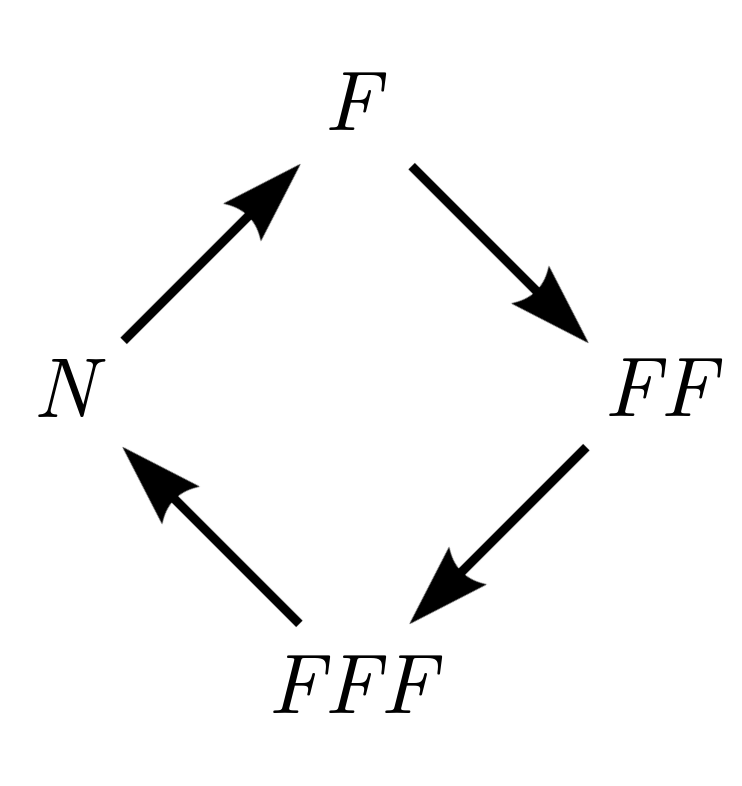
\includegraphics[scale=0.6]{Cayleygraph1.png}
\caption{Cayleygraph zu Erzeuger $\{ F \}$}
\label{Abbildung_CayleygraphF}
\end{figure}


Dieser Cayleygraph ist anschaulich, da der er nicht sonderlich komplex ist.
Die Untergruppe wird durch die Ebenendrehung $F$ erzeugt. Dadurch ergeben sich vier Elemente in der Trägermenge:
\begin{align*}
G_F = \{F, FF, FFF, N\}
\end{align*}
Jedes Element aus $G_F$ wird durch einen Knoten dargestellt. Die Pfeile zwischen den Knoten zeigen, welches Element sich durch das weitere Hinzufügen eines Erzeugers ergibt. In diesem Fall ist der Zyklus einer einzelnen Ebenendrehung zu sehen.


Im Vergleich dazu ist der Cayleygraph der durch $\{ FF, RR \}$ erzeugten Untergruppe komplexer (s. Abbildung \ref{Abbildung_CayleygraphFFRR}). Diese Untergruppe wurde in Abschnitt \ref{Abschnitt_UntergruppeFFRR} beschrieben.
Die roten Pfeile repräsentieren den Erzeuger $\{FF\}$, da es sich dabei in der Startkonfiguration um die rote Seite des Würfels handelt. Die blauen Pfeile repräsentieren den Erzeuger $\{RR\}$, da es sich dabei um die blaue Würfelseite handelt.
Elemente, die durch ein anderes Element in Kombination mit einem Erzeuger entstehen, sind durch einen Pfeil (Erzeuger) miteinander verbunden.

Anhand dieses Cayleygraphen kann beispielsweise abgelesen werden, dass die Züge $FFFF$ und $RRRR$ dem neutralen Element $N$ entsprechen. Von dem Knoten $FF$ führt ein roter Pfeil zu $N$. Die roten Pfeile repräsentieren den Erzeuger $FF$. Somit erzeugen $FFFF$ und $N$ die gleiche Würfelkonfiguration.

\begin{figure}[H]
\centering
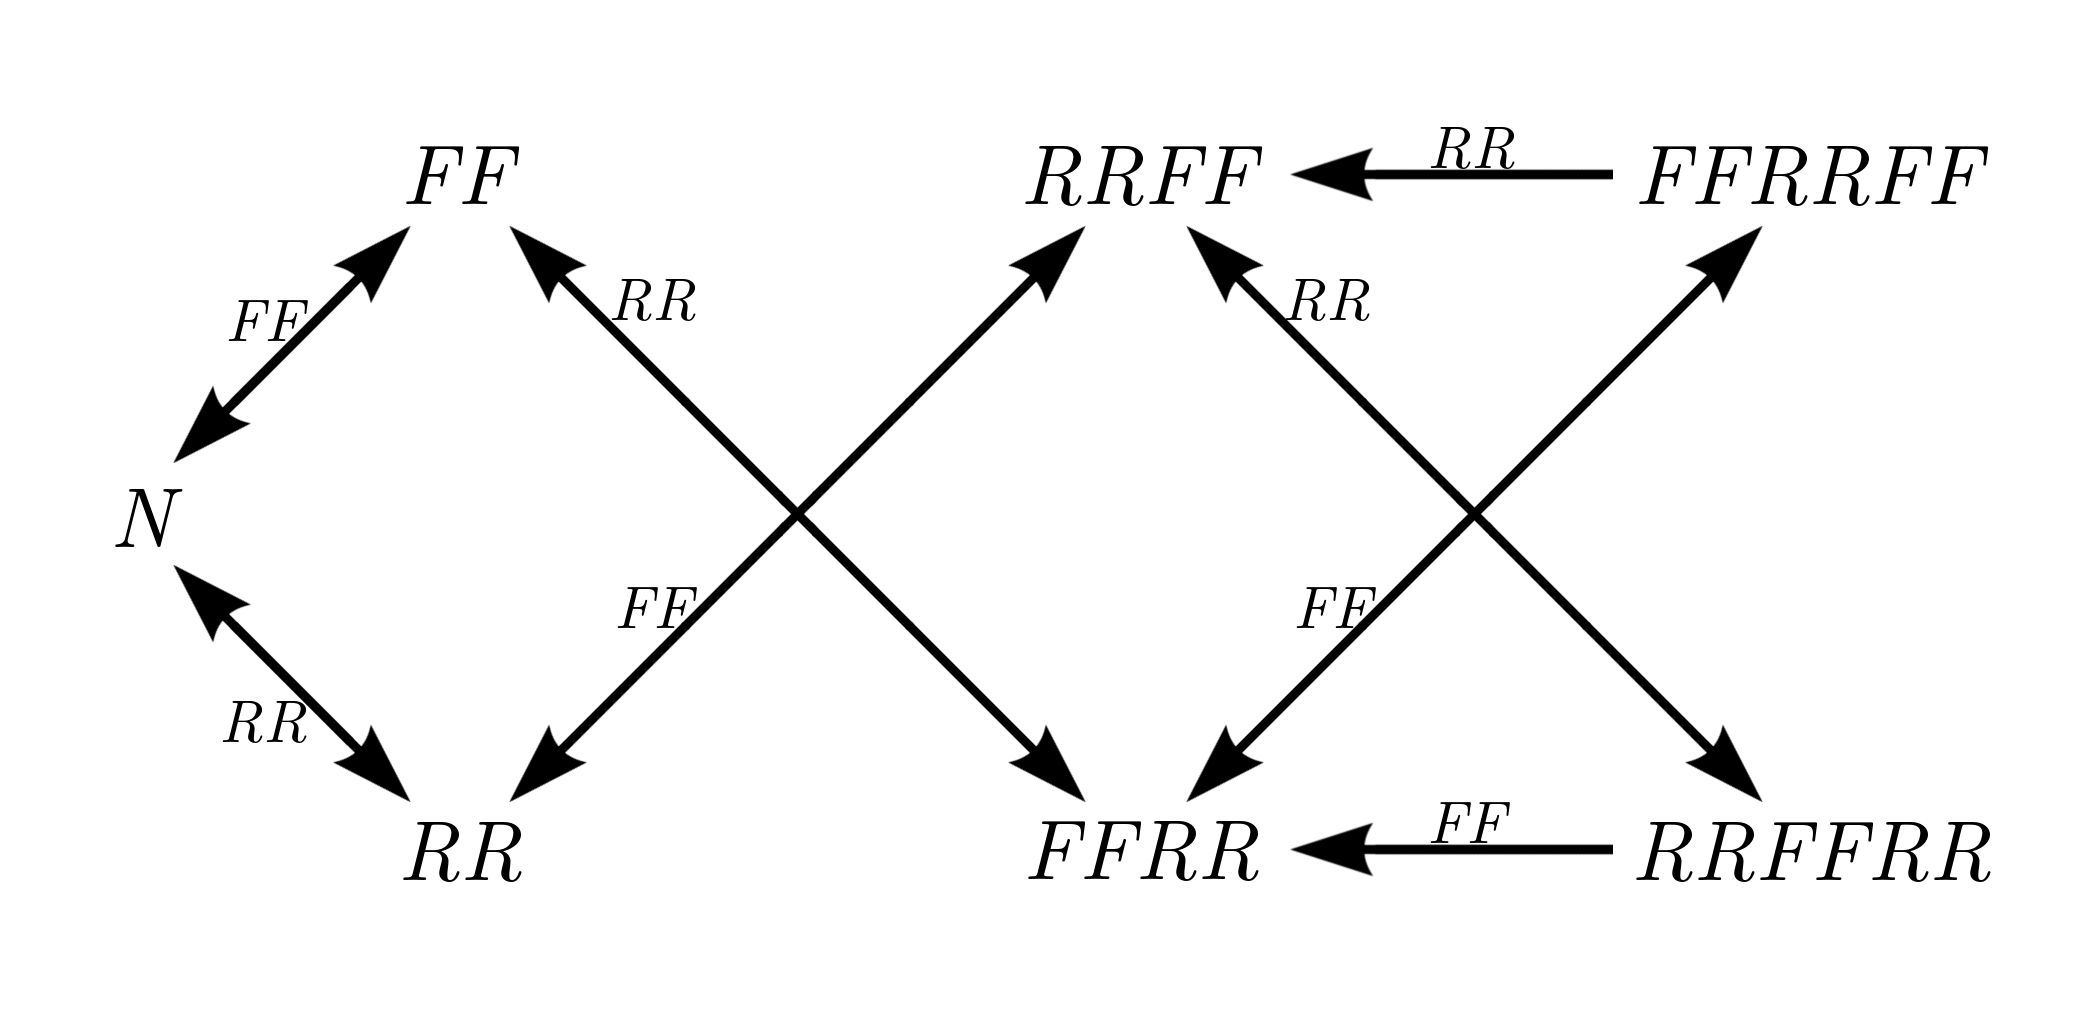
\includegraphics[scale=0.65]{Cayleygraph2.png}
\caption{Cayleygraph zu Erzeuger $\{ FF, RR \}$}
\label{Abbildung_CayleygraphFFRR}
\end{figure}

Dieser Cayleygraph ist wesentlich komplexer, als der Graph der Untergruppe $(G_F, \circ)$ (Abbildung \ref{Abbildung_CayleygraphF}). Trotzdem stellt er eine sehr kleine erzeugte Untergruppe dar, wenn man das mit der Größe der anderen erzeugbaren Untergruppen von $(\Gtwo, \circ)$ vergleicht. Die Untergruppen und Cayleygraphen können bei der Gruppe des \Ttwo Würfels (und des \Tthree Würfels) sehr groß werden. In Kapitel \ref{Kapitel_MinUntergruppe} wird die Untergruppe der minimalen, vollständigen Abbildung des Würfels definiert. Der Cayleygraph dieser Untergruppe wird in Abschnitt \ref{Abschnitt_CayleygraphMIN} beschrieben und enthält $3 \ 647 \ 160$ Knoten.



%
%
%
%
%
%
%
%=======================================================================================================
%
%
%
%
%
%
%
%
%
%
\newpage

\section{Valide Konfigurationen des Würfels}

\label{Kapitel_ValideKonfigurationen}

In diesem Kapitel wird die Anzahl der validen Würfelkonfigurationen berechnet -- sowohl anhand des physischen Würfels als auch mithilfe der Gruppe $(\Gtwo,\circ)$. Dazu wird die Mächtigkeit der Gruppe berechnet. Die Definition der Mächtigkeit und Beispiele sind in Abschnitt \ref{Abschnitt_MächtigkeitGruppe} zu finden. \\
Außerdem wird gezeigt, dass für die Ausrichtung $x$ der Steine $( \sum_{i= 1}^{8} \ x_i ) \mod 3 = 0$ gilt.

%
%
%
%
%
%
%
%
%
%=======================================================================================================
%
%
%
%
%
%
%
%
%
%
\subsection{Anzahl der validen Würfelkonfigurationen}
\label{Abschnitt_AnzahlKonfigurationen}

Im Folgenden wird die Anzahl der möglichen Würfelkonfigurationen anhand des Würfels brechnet. Nicht jede der theoretisch möglichen Würfelkonfigurationen kann auch wirklich durch Ebenendrehungen erreicht werden. Wie viele Möglichkeiten es im \Ttwo Würfel gibt und welche davon wirklich erreichbar sind, wird nun schrittweise anhand des Würfelaufbaus berechnet. 

Dazu wird zuerst die Anzahl der möglichen Steinpositionen berechnet:
Die Ecksteine können sich in jeder der acht Ecken befinden. Deshalb gibt es pro Eckstein 8 mögliche Positionen im Würfel. Da es 8 Ecksteine gibt, gibt es somit $8! = 1 \cdot 2 \cdot 3 \cdot 4 \cdot 5 \cdot 6 \cdot 7 \cdot 8 = 40\, 320$ mögliche Positionen für die Ecksteine. 

Außerdem können die Ecksteine gedreht sein, es können also verschiedene Farbflächen oben sein. Da die Steine aus 3 Farbflächen bestehen, können sieben davon durch Ebenendrehungen 3 verschiedene Ausrichtungen annehmen. Der achte Stein kann durch die Möglichkeit der Rotation des kompletten Würfels als richtig gedreht angenommen werden. Es gibt folglich $3^7 = 2187$ Möglichkeiten für die Ausrichtung der Ecksteine.

Da es keine Mittelsteine im Würfel gibt, reduziert die Rotation des Würfels die Möglichkeiten um den Faktor 24, denn es gibt $6$ Seiten, die jeweils $4$ Ausrichtungen haben können. Das sind dann $6 \cdot 4 = 24$. Alle $24$ Ausrichtungsmöglichkeiten sind in Anhang \ref{Anhang_RotationenDesWürfels} abgebildet.

Somit ergibt es $(3^7 \cdot 8!) \cdot \frac{1}{24}$ mögliche Konfigurationen für den Würfel. Das sind $3\, 674\, 160$ Konfigurationen.

%Die Anzahl der Würfelkonfigurationen ohne Berücksichtigung der Rotationen des Würfels liegt bei $8! \cdot 3^8 = 264 \, 539 \, 520$ \cite{MMFAA}. Unter der Berücksichtigung der Rotationen liegt die Anzahl bei $3\, 674\, 160$ Möglichkeiten.


%
%
%
%
%
%
%
%
%
%=======================================================================================================
%
%
%
%
%
%
%
%
%
%

\subsection{Mächtigkeit von \textit{G}$_{2 \times  2 \times 2}$} %\addcontentsline{toc}{subsection}{Mächtigkeit von \textit{G}$_{2 \times  2 \times 2}$}

\label{Abschnitt_MächtigkeitVonG}

Die Mächtigkeit der Gruppe $(\Gtwo,\circ)$ ist die Anzahl der Elemente von $\Gtwo$. Das wird auch als $|\Gtwo|$ bezeichnet. Die Mächtigkeit der Gruppe entspricht der Anzahl der validen Würfelkonfigurationen, da $\Gtwo$ die Äquivalenzklassen aller möglichen Züge enthält. Wenn zwei Züge mit gleicher Ausgangskonfiguration die gleiche Folgekonfiguration des Würfels hervorrufen, sind sie Repräsentanten der gleichen Äquivalenzklasse in $\Gtwo$. Somit bringt jedes Element von $\Gtwo$ den Würfel in eine andere Würfelkonfiguration und es sind keine äquivalenten Züge doppelt enhalten. Außerdem wurden die Äquivalenzklassen mit der Menge alle Züge des Würfels gebildet. Somit ist jeder mögliche Zug enthalten und $|\Gtwo|$ entspricht der Anzahl der validen Würfelkonfigurationen.

Da die Mächtigkeit der Gruppe $(\Gtwo,\circ)$ der Anzahl der validen Würfelkonfigurationen entspricht, setzt sie sich aus dem Produkt der Konfigurationsparameter $\sigma$ und $x$ zusammen. Außerdem müssen die Äquivalenzen bezüglich der Rotationen berücksichtigt werden.

$\sigma$ ist die Menge der bijektiven Funktionen für jede Ebenenrotation. Es sind die Übergänge der acht Würfelsteine als Permutationen enthalten. Da es $8$ Permutationsobjekte gibt, ist die Anzahl der Permutationsmöglichkeiten $8! = 40320$.

Der andere Parameter der Würfelkonfiguration ist der 8-dimensionale Vektor $x$. Jeder der Werte in $x$ ist aus der Menge $\{0,1,2\}$. Somit gibt es drei Möglichkeiten für jeden Wert im Vektor. Das ergibt dann $3^8 = 6561$ mögliche Konfigurationen des Vektors.

Ohne Berücksichtigung der Rotationen wird ein Wert von $40320 \cdot 6561 = 264 \, 539 \, 520$ möglichen Konfigurationen erreicht. 
Da durch die Rotationen eine der Steinausrichtungen in $x$ als richtig angenommen werden kann, wird $264 \, 539 \, 520$ durch drei geteilt und ergibt dann $88 \, 179 \, 840$. 
Außerdem gibt es $6 \cdot 4 = 24$ Rotationsmöglichkeiten, die in den Äquivalenzklassen berücksichtigt werden. Alle 24 Rotationsmöglichkeiten sind in Anhang \ref{Anhang_RotationenDesWürfels} abgebildet. Somit muss $88 \, 179 \, 840$ durch $24$ geteilt werden, um die Mächtigkeit der Gruppe $(\Gtwo,\circ)$ zu berechnen. $|\Gtwo|$ ist dann $88 \, 179 \, 840 \div 24 = 3\, 674\, 160$.

Die Mächtigkeit der Gruppe $(\Gtwo,\circ)$ entspricht der Anzahl der validen Würfelkonfigurationen: $3\, 674\, 160$.



%
%
%
%
%
%
%
%
%
%
%=======================================================================================================
%
%
%
%
%
%
%
%
%
%
\subsection{Ausrichtung der Steine (modulo 3)}

\label{Abschnitt_Modulo3}

Die Konfiguration des Würfels ist als $C=(\sigma, x)$ definiert. In diesem Abschnitt wird gezeigt, dass bei jeder validen Würfelkonfiguration für die Werte des Vektors $x$ folgendes gilt: 
\begin{displaymath}
\left( \sum_{i= 1}^{8} \ x_i \right) \hspace*{-0.7em} \mod 3 = 0 
\end{displaymath} 

Sei $C'=(\sigma', x')$ eine Nachfolgekonfiguration der Konfiguration $C=(\sigma, x)$.  Dabei ist $Z$ einer der Züge aus $\Gtwo$.  
\begin{align*}
{(\sigma, x) \cdot Z = (\sigma', x')}
\end{align*}
Für diese Vektoren $x$ und $x'$ gilt dann:
\begin{align*}
(\sum_{i= 1}^{8} \ x_i') \hspace*{-0.5em} \mod 3 = (\sum_{i= 1}^{8} \  x_i) \hspace*{-0.5em} \mod 3 = 0
\end{align*}

%Die Veränderung der Vektoreinträge durch die Grundzüge des Würfels, ausgehend von der Startkonfiguration, kann auch in dieser Tabelle gesehen werden: 
%\vspace*{1em}

%\begin{adjustbox}{width=1\textwidth,center}

%\begin{tabular}{cllcc}
%\toprule
% \textbf{Zug} $\boldsymbol{Z}$ & \hspace*{2.2cm}$\boldsymbol{x}$ & \hspace*{2cm} $\boldsymbol{x'}$ &  $\boldsymbol{\sum_{i= 1}^{8} x_i'} \ \ \ $ & $\boldsymbol{\mod 3}$ \\
%\midrule
%
%\textit{U} & $(x_1, x_2, x_3, x_4, x_5, x_6, x_7, x_8)$ & $(x_3, x_1, x_4, x_2, x_5, x_6, x_7, x_8)$ & 0 & 0 \\
%
%\textit{D} & $(x_1, x_2, x_3, x_4, x_5, x_6, x_7, x_8)$ & $(x_1, x_2, x_3, x_4, x_6, x_8, x_5, x_7)$ & 0 & 0 \\
%
%\textit{R} & $(x_1, x_2, x_3, x_4, x_5, x_6, x_7, x_8)$ & $(x_1, 2, x_3, 1, x_5, 1, x_7, 2)$ & 6 & 0 \\
%
%\textit{L} & $(x_1, x_2, x_3, x_4, x_5, x_6, x_7, x_8)$ & $(1, x_2, 2, x_4, 2, x_6, 1, x_8)$ & 6 & 0 \\
%
%\textit{F} & $(x_1, x_2, x_3, x_4, x_5, x_6, x_7, x_8)$ & $(x_1, x_2, 1, 2, x_5, x_6, 2, 1)$ & 6 & 0 \\
%
%\textit{B} & $(x_1, x_2, x_3, x_4, x_5, x_6, x_7, x_8)$ & $(2, 1, x_3, x_4, 1, 2, x_7, x_8)$ & 6 & 0 \\
%\bottomrule
%
%\end{tabular}
%
%\end{adjustbox}
%
%
%Sowohl für die Startkonfiguration als auch die Folgekonfiguration nach dem Ausführen eines Grundzuges gilt 
%\begin{align*}
%(\sum_{i= 1}^{8} \ x_i) \mod 3 = 0
%\end{align*}


Der Würfel kann durch einen der Grundzüge des Würfels oder einer Kombination der Grundzüge verändert werden. Die Veränderungen des Vektors $x$ durch das Ausführen der Grundzüge sind in der folgenden Tabelle detailliert zu sehen. Die Variable $s$ beschreibt dabei die Veränderung der Summe der Vektoreinträge. In Abschnitt \ref{Abschnitt_AusrichtungDerSteine} sind die Funktionen definiert, die die Veränderungen des Vektor $x$ für jeden der Züge realisieren. 
\ \\


\begin{adjustbox}{width=1\textwidth,center}
\begin{tabular}{c l c c }
\toprule

\textbf{Zug} $\boldsymbol{Z}$ & \textbf{Vektor} $\boldsymbol{x}$ & $\boldsymbol{s}$  & $\boldsymbol{\mod 3}$ \\

\midrule

$U$ & $(x_3, x_1,x_4,x_2,x_5,x_6,x_7,x_8)$ & +0 & 0 \\

$D$ & $(x_1,x_2,x_3,x_4,x_6,x_8,x_5,x_7)$ & +0 & 0 \\

$R$ & $(x_1,(x_4 + 2) \hspace*{-0.5em} \mod 3,x_3,(x_8 + 1) \hspace*{-0.5em} \mod 3,x_5,(x_2 +1) \hspace*{-0.5em} \mod 3,x_7,(x_6 + 2) \hspace*{-0.5em} \mod 3)$ & +6 & 0 \\

$L$ & $((x_5 + 1) \hspace*{-0.6em} \mod 3, x_2, (x_1 + 2) \hspace*{-0.6em} \mod 3, x_4, (x_7 + 2) \hspace*{-0.6em} \mod 3, x_6, (x_3 + 1) \hspace*{-0.6em} \mod 3, x_8)$ & +6 & 0 \\

$F$ & $(x_1, x_2, (x_7 +1) \hspace*{-0.6em} \mod 3, (x_3 + 2)  \hspace*{-0.6em} \mod 3, x_5, x_6, (x_8 +2)  \hspace*{-0.6em} \mod 3, (x_4 + 1) \hspace*{-0.6em} \mod 3$ & +6 & 0 \\

$B$ & $(x_2 +2) \hspace*{-0.6em} \mod 3, (x_6 + 1)  \hspace*{-0.6em} \mod 3, x_3, x_4,(x_1 + 1), (x_5 + 2)  \hspace*{-0.6em} \mod 3, x_7, x_8)$ & +6 & 0 \\

\bottomrule
\end{tabular}
\end{adjustbox}
\ \\

Jede valide Würfelkonfiguration $C$ kann ausschließlich durch Züge erreicht werden. Züge bestehen aus Elementen der Menge $\{U, D, R, L, F, B\}$. In der Startkonfiguration ist der Summe der Vektoreinträge $0$. Der Vektor $x$ ist dabei $(0,0,0,0,0,0,0,0)$ und die Summe der Einträge ist somit 0. Es gilt 
\begin{align*}
(\sum_{i= 1}^{8} \ (0,0,0,0,0,0,0,0)) \hspace*{-0.5em} \mod 3 = 0
\end{align*}
Bei jedem der Grundzüge aus $\{U, D, R, L, F, B\}$ wird die Summe der Vektoreinträge um den Wert von $s$ verändert. Die Variable $s$ ist bei den Grundzügen entweder 0 oder 6. Es gilt demnach auch:
\begin{align*}
s \hspace*{-0.5em} \mod 3 = 0
\end{align*}
Somit muss die Summe $s$ der Vektoreinträge immer 0 sein, wenn modulo 3 gerechnet wird, da jeder Zug $Z$ aus einem der Grundzüge aus $\{U, D, R, L, F, B\}$ oder einer Kombination dieser besteht. Jedes Vielfache von 6 und 0 ergibt 0, wenn modulo 3 gerechnet wird. Es gilt demnach:
\begin{align*}
(k \cdot s) \hspace*{-0.5em} \mod 3 = 0 \textit{ für } k \in \mathbb{N}
\end{align*}
Und somit gilt auch:
\begin{align*}
(\sum_{i= 1}^{8} \ x_i') \hspace*{-0.5em} \mod 3 = (\sum_{i= 1}^{8} \  x_i) \hspace*{-0.5em} \mod 3 = 0.
\end{align*}

Da in Abschnitt \ref{Abschnitt_RotationDesWürfels} gezeigt wurde, dass die Rotationen auch als Kombination von Zügen definiert werden können, gilt die Aussage auch für jede Rotation des Würfels.


%Für jede valide Würfelposition gilt folglich ${(\sum_{i = 1}^{8} \ x_i') \mod 3 = (\sum_{i = 1}^{8} \  x_i) \mod 3 }$. 
%Wenn es eine valide Konfiguration $C'=(\sigma', x')$ gibt, für die $\sum_{i = 1}^{8} x_i' \mod 3 = 0$ gilt, dann gibt es einen Zug $Z \in \Gtwo$, so dass $Z \cdot C'$ die Steine in die Konfiguration $(1,x)$ bringt Alle Steine befinden sich dann an der richtigen Position, sind aber nicht korrekt ausgerichtet. 
%Von dieser Konfiguration $(1,x)$ ausgehend gibt es einen Zug $Z \in \Gtwo$, so dass alle Eckstücke richtig ausgerichtet sind. Dann ergibt sich die Konfiguration $(1, 0)$ und alle Eckstücke sind in der richtigen Ausrichtung und Position. Der Würfel befindet sich dann in der Startkonfiguration. 
%
%
%
%
%
%
%
%
%
%
%=======================================================================================================
%
%
%
%
%
%
%
%
%
%
\newpage


\section{Lösung des Würfels}

\label{Kapitel_Lösung}

Die übliche, händische Methode zum Lösen eines Zauberwürfels erfolgt durch das Kombinieren verschiedener Ebenendrehungen. Diese werden als eine Einheit angewendet und verändern die Konfiguration des Würfels dann spezifisch. 
Es gibt beispielsweise eine Kombination, die 3 der 4 Ecken der oberen Ebene untereinander im Uhrzeigersinn tauscht und deren Ausrichtung dabei nicht verändert. 

In diesem Kapitel wird die Anzahl der $2$-Zykel der Züge untersucht und Kommutatoren erklärt.
Dann wird beispielhaft ein Lösungsvorgang eines Menschens schrittweise beschrieben und erklärt.
Außerdem werden Muster des Würfels algorithmisch beschrieben und grafisch dargestellt.
Danach werden verschiedene Lösungsalgorithmen des \Tthree \textit{Cubes} auf den \Ttwo Würfel übertragen.

%
%
%
%
%
%
%
%
%
%
%=======================================================================================================
%
%
%
%
%
%
%
%
%
%
\subsection{Anzahl der 2-Zykel}

Die Position der Würfelsteine wird durch die Permutationsfunktionen $\sigma$ beschrieben.  $\sigma$ besteht aus verschiedenen Zykeln in Abhängigkeit von der Position der Steine. Das wurde in Abschnitt \ref{Abschnitt_PositionenDerSteineImWürfel} definiert und beschrieben. Jeder $n$-Zykel kann als Produkt von $2$-Zykeln geschrieben werden. Wenn $n$ dabei gerade ist, hat das dazugehörige $2$-Zykel-Produkt eine ungerade Anzahl an $2$-Zykeln und anders herum. \cite{TD}

Jede Würfelkonfiguration kann durch eine Kombination der Ebenendrehungen $U, D, F, B, L, R$ (und der Rotationen des Würfels) erreicht werden. 
Die Zykel der einzelnen Ebenendrehungen des Würfels sind im Folgenden als Produkt von $2$-Zykeln geschrieben:
\begin{alignat*}{2}
\sigma_U &  = \ ( \textit{ulf} \ \textit{ulb} \ \textit{urb} \ \textit{urf} ) &&  = \ ( \textit{ulf} \ \textit{ulb} )   \ 
( \textit{ulf} \ \textit{urb} )  \ 
( \textit{ulf} \  \textit{urf} )\\

\sigma_D & = \ ( \textit{dlf} \ \textit{drf} \ \textit{drb} \ \textit{dlb} )  && = \ ( \textit{dlf} \ \textit{drf} )  \ 
( \textit{dlf} \ \textit{drb}  )  \ 
( \textit{dlf} \ \textit{dlb} )\\

\sigma_F & = \ ( \textit{ulf} \ \textit{urf} \ \textit{drf} \ \textit{dlf} )  && = \ ( \textit{ulf} \ \textit{urf} ) \ 
( \textit{ulf} \ \textit{drf} ) \ 
( \textit{ulf}  \ \textit{dlf} ) \\

\sigma_B & = \ ( \textit{ulb} \ \textit{dlb} \ \textit{drb} \ \textit{urb} )  && = \ ( \textit{ulb} \ \textit{dlb} ) \ 
( \textit{ulb} \  \textit{drb} ) \ 
( \textit{ulb}  \ \textit{urb} )\\

\sigma_L & = \ ( \textit{ulb} \ \textit{ulf} \ \textit{dlf} \ \textit{dlb} )  && = \ ( \textit{ulb} \ \textit{ulf} )  \ 
( \textit{ulb} \ \textit{dlf}  )  \ 
( \textit{ulb} \ \textit{dlb} ) \\

\sigma_R & = \ ( \textit{urb} \ \textit{drb} \ \textit{drf} \ \textit{urf} ) && = \  ( \textit{urb} \ \textit{drb}  )  \ 
( \textit{urb} \  \textit{drf} )  \ 
( \textit{urb} \ \textit{urf} )  \
\end{alignat*}
Anhand der Funktionen der Grundzüge ist ersichtlich, dass jeder Grundzug durch einen $4$-Zykel definiert ist.
Jeder $4$-Zykel kann als Produkt aus drei $2$-Zykeln geschrieben werden. 
Die Anzahl der $2$-Zykel einer einzelnen Ebenendrehung ist demnach ungerade. Die Anzahl der $2$-Zykel eines Zuges, der aus zwei Ebenendrehungen besteht ist demnach gerade.
Beispielsweise hat der Zug $LF$ eine gerade Anzahl an $2$-Zykeln:
\begin{align*}
\sigma_{LF} & = (\textit{ulb} \ \textit{urf} \ \textit{drf} \ \textit{dlf} \ \textit{dlb}) \\
 & =  (\textit{ulb} \ \textit{urf}) \ (\textit{ulb} \ \textit{drf}) \ (\textit{ulb} \ \textit{dlf}) \ (\textit{ulb} \ \textit{dlb})
\end{align*}

Die Zykel treffen ausschließlich eine Aussage über die Position der Steine im Würfel. Die Rotation wird durch den Vektor $x$ dargestellt und hier nicht berücksichtigt. 

Bei dem \Tthree Würfel ist die Anzahl der $2$-Zykel jeder Permutation gerade, deshalb gibt es keinen Zug, der genau zwei Steine im Würfel tauscht \cite{TD}. Ein Zug, der genau zwei Steine tauscht, wird durch \textit{einen} $2$-Zykel dargestellt -- das wäre eine ungerade Anzahl an $2$-Zykeln. Im Gegensatz zum \Tthree Würfel kann die Anzahl der $2$-Zykel des \Ttwo Würfels ungerade sein und somit es gibt für diesen Würfel Algorithmen, die die Position von genau zwei Steinen tauschen. Diese Algorithmen sind in Abschnitt \ref{Abschnitt_AlgorithmenZweiteEbene} beschrieben. 

%
%
%
%
%
%
%
%
%
%
%=======================================================================================================
%
%
%
%
%
%
%
%
%
%
\subsection{Kommutatoren}
\label{Abschnitt_Kommutatoren8}

Kommutatoren wurden in Abschnitt Abschnitt \ref{Abschnitt_Kommutator} erklärt. Der Kommutator von zwei Zügen $Y, Z$ der Gruppe $(\Gtwo, \circ)$ ist demnach definiert als:
\begin{align*}
[Y,Z]=YZY^{-1}Z^{-1}
\end{align*}
Kommutierende Elemente sind Elemente, die als Kommutator das neutrale Element einer Gruppe ergeben. Das neutrale Element ist hier der leere Zug $N$.
\begin{align*}
[Y,Z]= N\ \Rightarrow \textit{ $Y$ und $Z$ sind kommutierende Elemente}
\end{align*}
Zwei gleiche Züge $Y, Z$ der Gruppe $(\Gtwo, \circ)$ kommutieren:
\begin{align*}
\forall \ Y, Z \in \Gtwo, Y = Z \ . \ [Y, Z] = N
\end{align*}
Zu dieser Aussage folgt ein Beweis. Zur besseren Übersichtlichkeit wird dabei $[Y,Z]$ mit $Y=Z$ nun als $[Z,Z]$ geschrieben.
\begin{align*}
\forall \ Z \in \Gtwo\ . \ [Z, Z] = N
\end{align*}
Auf eine Konfiguration $C$ angewandt, ist der Kommutator zweier gleicher Elemente im Folgenden definiert:
\begin{align*}
\forall \ Z \in \Gtwo\ . \ C \cdot [Z, Z] = C
\end{align*}
Das kann dann folgendermaßen umgeformt werden:
\begin{align*}
C \cdot [Z, Z] & = C \cdot ZZZ^{-1}Z^{-1} \\
& = C \cdot Z(ZZ^{-1})Z^{-1} \\
& = C \cdot Z(N)Z^{-1} \\
& = C \cdot ZZ^{-1} \\
& = C \cdot N \\
& = C
\end{align*}
Somit kommutieren alle Zugpaare aus $\Gtwo$, die aus zwei gleichen Zügen bestehen.


Es kommutieren nicht ausschließlich gleiche Zugpaare, sondern auch Züge, die gegenüberliegende Ebenen beeinflussen. Somit bewegen sie nicht dieselben Steine. Diese sogenannten \textit{elementfremden Zykel} kommutieren \cite{OS}. Auch bei dem Vektor $x$ werden dann keine gemeinsamen Einträge beeinflusst.
Das sind dann die folgenden Kommutatoren, mit $n, m \in \mathbb{N}$:
\begin{align*}
[U^n, D^m] \ \ \ \  \ \ \ [F^n, B^m] \ \ \ \ \ \ \ [L^n, R^m] \\
[D^n, U^m] \ \ \ \ \ \ \  [B^n, F^m] \ \ \ \ \ \ \ [R^n, L^m] 
\end{align*}

Da die Zugpaare nicht dieselben Steine beeinflussen, ist es nicht relevant, dass die Gruppe nicht kommutativ ist. Durch den Aufbau des Kommutators werden beide Züge ausgeführt und wieder invertiert.


Wenn zwei Züge $Y, Z \in \Gtwo$ nicht kommutieren, kann anhand der Komplexität des Kommutators bis zu einem gewissen Grad eine Aussage darüber getroffen werden, wie groß die Veränderung der Würfelkonfiguration nach dem Ausführen von $[Y, Z]$ ist. 
Zur Veranschaulichung folgt nun ein Beispiel mit den Zügen $L$ und $F$ und der Startkonfiguration $C = (1,0)$:
\begin{align*}
C \cdot  [L, F] = C \cdot LFL^{-1}F^{-1}
\end{align*}
Dabei verändern vier der acht Steine im Würfel ihre Position und Ausrichtung. Die anderen vier bleiben unverändert. 
% Die folgenden Permutationen ergeben sich durch das Ausführen von $[L, F]$.
%
%\begin{center}
%\begin{tabular}{lcccccccc}
%\toprule
%\textbf{Zug} & \textbf{ulb} & \textbf{urb} & \textbf{ulf} & \textbf{urf} & \textbf{dlb} & \textbf{drb} & \textbf{dlf} & \textbf{drf} \\
%
%\midrule
%$L$ & ulf & \textcolor{gray}{urb} & dlf & \textcolor{gray}{urf} & ulb & \textcolor{gray}{drb} & dlb & \textcolor{gray}{drf} \\
%
%$F$ & urf & \textcolor{gray}{urb} & ulf &  drf & \textcolor{gray}{ulb} & \textcolor{gray}{drb} & \textcolor{gray}{dlb} & dlf \\
%
%$L^{-1}$ & \textcolor{gray}{urf} & \textcolor{gray}{urb} & ulb & \textcolor{gray}{drf} & dlb & \textcolor{gray}{drb} & dlf & ulf \\
%
%$F^{-1}$ \: & ulf & \textcolor{gray}{urb} & \textcolor{gray}{ulb} & urf & \textcolor{gray}{dlb} & \textcolor{gray}{drb} & drf & dlf\\
%\bottomrule
%\end{tabular}
%\end{center}
%
%
%Wenn nun die Kopfzeile der Tabelle und die unterste Zeile verglichen werden, zeigt sich, dass \textit{urb}, \textit{urf}, \textit{dlb} und \textit{drb} wieder an ihrer Ausgangsposition sind. Die anderen vier Steine (\textit{ulf}, \textit{ulb}, \textit{urf} und \textit{dlf}) haben die Positionen gewechselt: \\
%\\
%\hspace*{1.5cm } $\textit{ulb} \mapsto \textit{ulf}$ \hspace*{1.5cm }$\textit{ulf}  \mapsto \textit{ulb}$ \hspace*{1.5cm } $\textit{dlf} \mapsto \textit{drf}$ \hspace*{1.5cm } $\textit{drf} \mapsto \textit{dlf}$
%\\
%\\

Die Folgekonfiguration ist im Folgenden zu sehen, mit $C=(1,0)$:
\begin{align*}
C \cdot [L, F] = (( \textit{ulb} \ \textit{ulf} ) \ (\textit{dlf} \ \textit{drf} ), (0,0,2,0,0,0,0,1) )
\end{align*}
%Daraus ergibt sich $C \cdot \lbrack L, F \rbrack  = (( \ \textit{ulb} \ \textit{ulf} \ )(\ \textit{dlf} \ \textit{drf} \ ), (0,0,2,0,0,0,0,1) )$ in der Zykelschreibweise. 
Es haben demnach zwei Steinpaare ihre Position getauscht und ihre Ausrichtung verändert. Im Vergleich dazu werden beispielsweise bei dem Kommutator von $\lbrack L, R \rbrack$ keine Steinpositionen verändert, da $L$ und $R$ keine gemeinsamen Steine beeinflussen.

Um aussagekräftigere Ergebnisse zu der Kommutativität der Zugpaare zu bekommen, müsste eine größere Menge der Kommutatoren berechnet und verglichen werden. Das ist allerdings zu Umfangreich für den Rahmen dieser Arbeit. Die Berechnung und Auswertung der Kommutatoren sollte maschinell erfolgen.

%
%
%
%
%
%
%
%
%
%
%=======================================================================================================
%
%
%
%
%
%
%
%
%
%
\subsection{Lösungsansätze}
\label{Abschnitt_Lösungsansätze}

Für die Lösung des Würfels sind Züge nützlich, die lediglich wenige Steine beeinflussen. So können dann gezielt bestimmte Steine gedreht oder getauscht werden. 

Es gibt verschiedene Vorgehensweisen, um den Würfel zu lösen. Üblicherweise werden die Ebenen des Würfels nacheinander gelöst. 
Für die Lösungsalgorithmen ist die Farbe der ersten Seite nicht relevant. Es wird aber häufig mit weiß begonnen, da die Anordnung der Farben so leichter zu merken ist. Dann kann schneller gesehen werden, in welche Ebene ein Stein gehört. \cite{RF} Deshalb wird im weiteren Verlauf dieser Arbeit bei der Lösung mit der weißen Seite begonnen.

Die beiden unten beschriebenen Lösungsansätze führen nicht zu einer optimalen Lösung des Würfels. Mehr zu der optimalen Lösung findet sich am Ende von Abschnitt \ref{Abschnitt_LösungBeispiel} und in Abschnitt \ref{Abschnitt_MinLösung}. Außerdem ist zu beachten, dass es eine Vielzahl weiterer Lösungsansätze gibt.

\subsubsection*{Ebenen nacheinander vollständig lösen}

Einer der Lösungsansätze geht so vor, dass die beiden Ebenen nacheinander vollständig gelöst werden. Dazu wird zuerst die erste Ebene und danach die zweite vollständig gelöst. Die erste Ebene kann durch simplere Züge gelöst werden als die zweite Ebene. Grund dafür ist, dass die Anordnung der Steine der zweiten Ebene beim Lösen der ersten Ebene noch nicht relevant ist. Beim Lösen der zweiten Ebene müssen komplexere Züge genutzt werden, um den gelösten Zustand der ersten Ebene beizubehalten. 

Eine gängige Lösungsmethode für die zweite Ebene sieht vor, dass zuerst alle Steine der Ebene richtig ausgerichtet werden. Dann sind alle $x_i=0$. Danach werden die Positionen noch getauscht. Die Würfelkonfiguration ist dann $(1,0)$ und der Würfel gelöst.

Dieses ebenenweise Vorgehen wird üblicherweise bei dem \Tthree Würfel angewandt und wurde hier auf den \Ttwo Würfel übertragen: Beim \Tthree Würfel wird zuerst die obere Ebene gelöst, dann die Mittlere, gefolgt von der Unteren. Wird dieses Vorgehen auf den \Ttwo Würfel übertragen, können sämtliche Lösungsschritte, die die Kanten beeinflussen, ignorieren, da der \Ttwo Würfel keine Kantsteine hat. Außerdem gibt es keine mittlere Ebene und die entsprechenden Lösungsschritte des \Tthree Würfels werden ebenfalls nicht auf den \Ttwo Würfel übertragen.

Dieser Lösungsansatz wird auch \textit{CFOP-Methode}\footnote{Die Abkürzung \textit{CFOP} bezieht sich auf das Lösen des \Tthree Würfels und steht für: \textit{Cross}, \textit{First two layers}, \textit{Orient last layer} und \textit{Permute last layer}. Das beschreibt das Vorgehen dieser Methode. \cite{DDJT}} oder \textit{Fridrich-Methode}\footnote{Nach Jessica Fridrich benannt, die diese Methode erfunden hat. $[$Jessica Fridrich, persönliche Korrenpondenz per E-Mail, s. Anhang \ref{Anhang_JessicaFridirch}$]$} genannt \cite{DDJT}.
Er wird in Abschnitt \ref{Abschnitt_LösungBeispiel} anhand eines Beispiels schrittweise ausgeführt und erklärt. Außerdem werden die Algorithmen für die beiden Ebenen in den Abschnitten \ref{Abschnitt_AlgorithmenErsteEbene} und \ref{Abschnitt_AlgorithmenZweiteEbene} beschrieben. Dies kann als eine Anleitung zum Lösen des Würfels dienen.

\subsubsection*{Steine ausrichten und dann positionieren}

Bei einem anderen Lösungsansatz werden zuerst alle Steine der ersten Ebene richtig ausgerichtet. Es gibt dann eine weiße Seite, die aus vier weißen Farbflächen besteht. Die Position der Steine ist dabei jedoch nicht relevant. Danach werden alle Steine der zweiten Ebene ausgerichtet. Auch hier ist die Position nicht relevant. Es gibt dann eine weiße und eine gelbe Seite, die anderen vier Seiten sind allerdings nicht gelöst, da die Steinposition noch nicht berücksichtig wurde.
Wenn alle Steine korrekt ausgerichtet sind und der Vektor $x=0$ ist, werden sie untereinander getauscht und der Würfel wird so gelöst. Dieses Vorgehen wird Ortega-Methode genannt \cite{RF2}.


%Bei einem anderen Lösungsansatz werden die Steine zuerst in die richtige Position gebracht. Die Permutationsfunktion $\sigma$ ist dann 1. Danach wird die Ausrichtung der Steine noch verändert. (?) Der Würfel ist dann wieder in der Startkonfiguration.

%Ein Beispiel für einen Zug dieses Lösungsansatzes ist $\lbrack R, U \rbrack \lbrack R^{-1}, F \rbrack$. Dabei werden zwei Steine der oberen Ebene gedreht und drei Steine verändern ihre Position. Dieser Zug kann für die Lösung der zweiten Ebene genutzt werden, ohne dabei die erste Ebene zu verändern. \cite{RF2} 
%In Abbildung \ref{Abbildung_AusrichtungEbene2} ist zu sehen, wie der Würfel bei der Ausgangsposition (links) durch den Zug $\lbrack R, U \rbrack \lbrack R^{-1}, F \rbrack$ verändert wird. Die Steine der oberen Ebene werden dabei ausgerichtet.

%\begin{figure}[h]
%\centering
%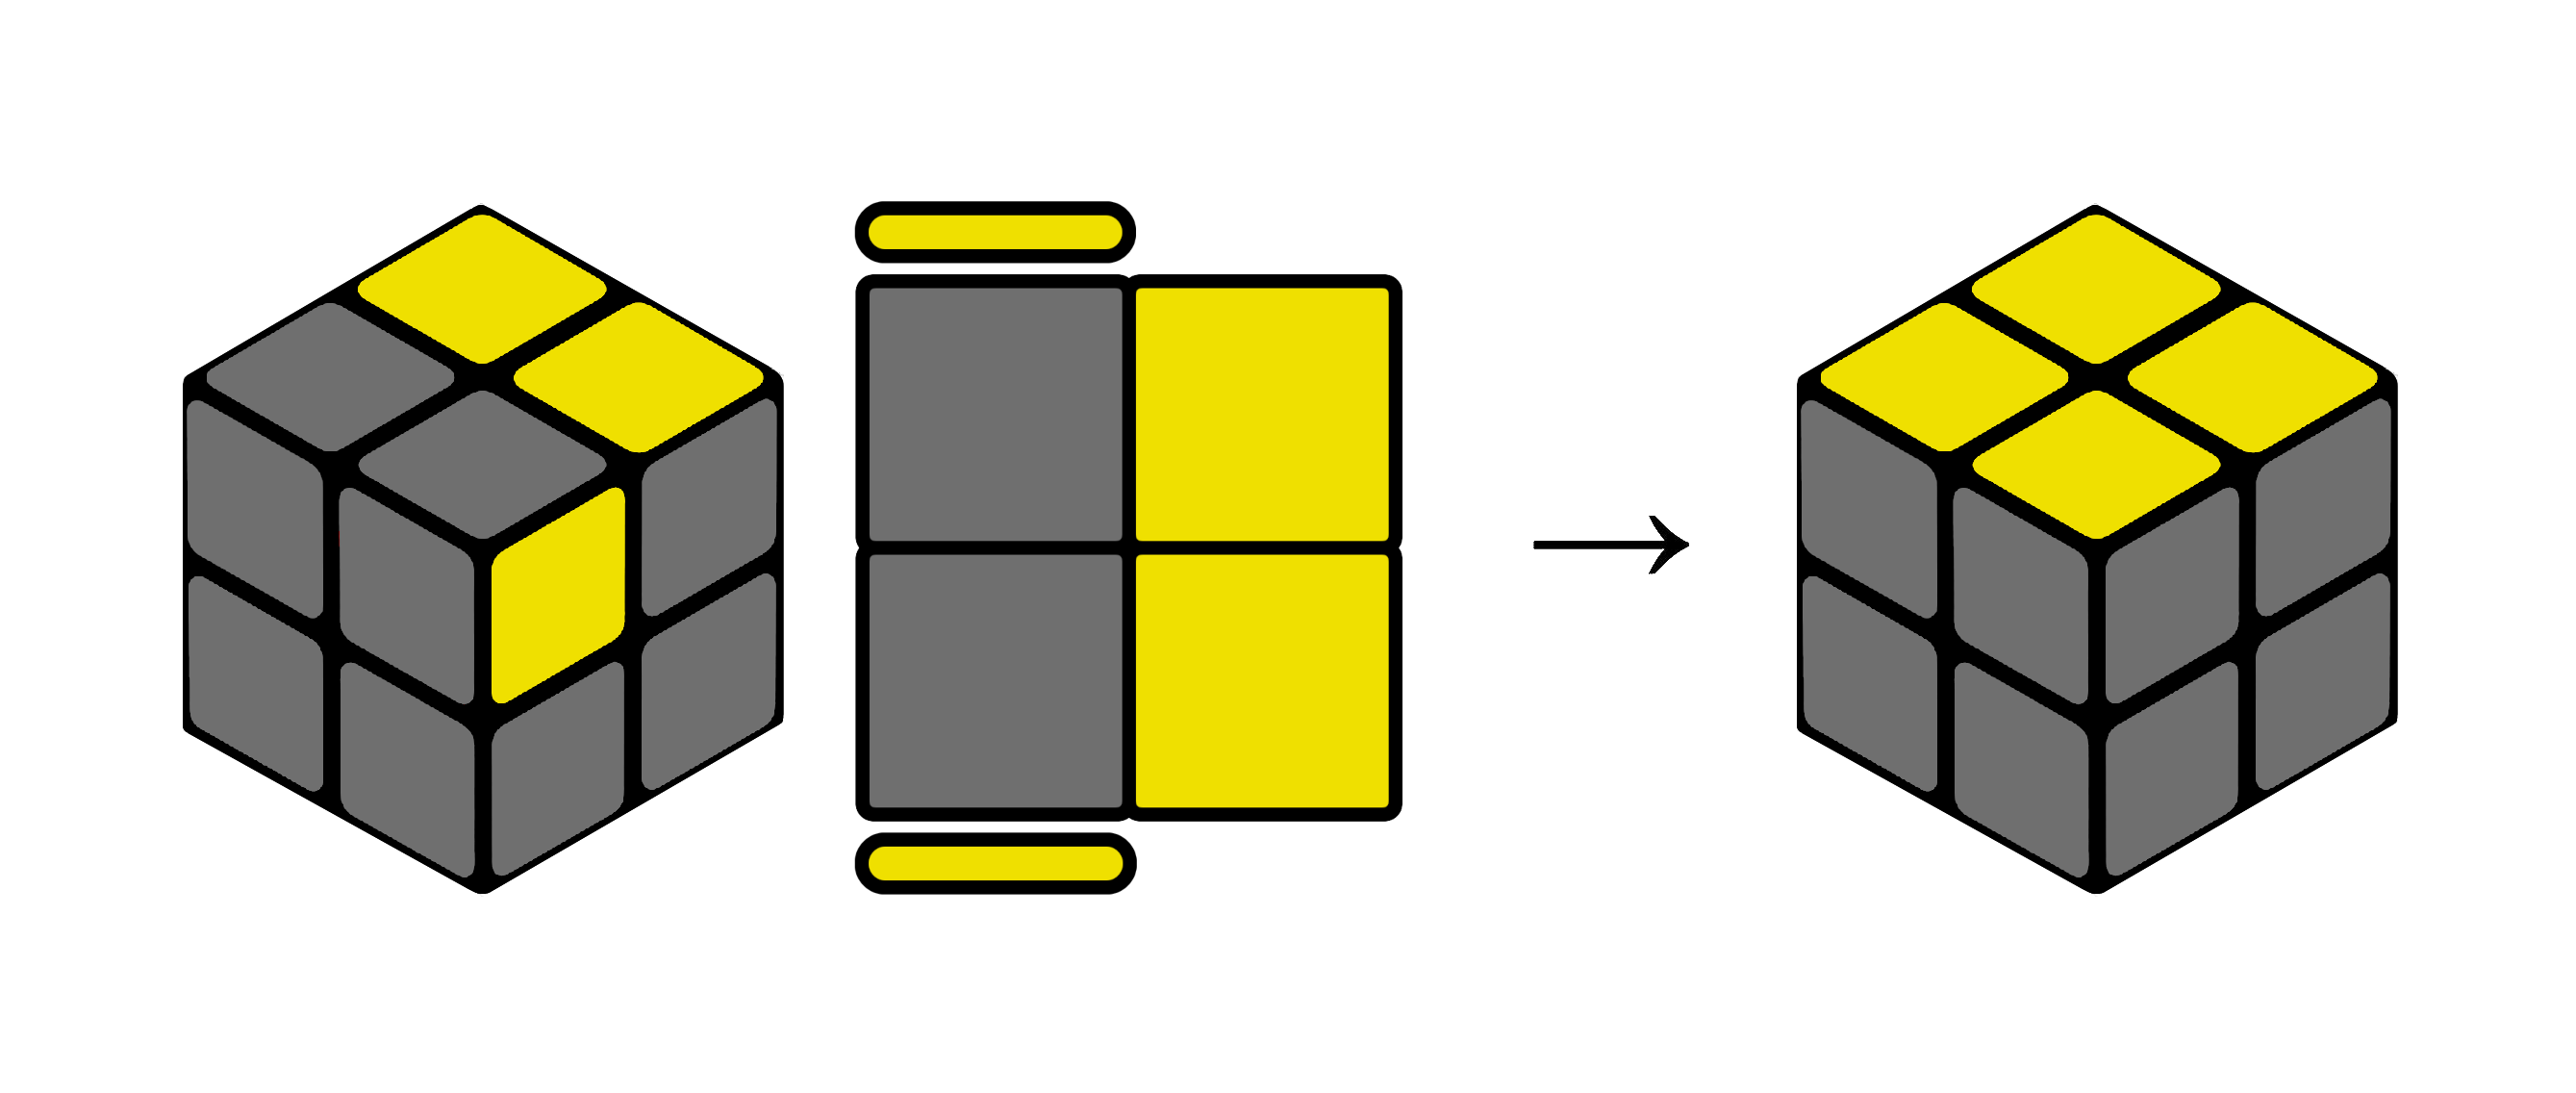
\includegraphics[scale=0.12]{isiakanm.png}
%\caption{Ausrichtung der zweiten Ebene (Beispiel)}
%\label{Abbildung_AusrichtungEbene2}
%\end{figure}

%$\lbrack R, U \rbrack \lbrack R^{-1}, F \rbrack$ kann auch als Zykel geschrieben werden: $( \ \textit{ulb} \ \textit{ulf} \ \textit{urb} \ )$. 
%
%
%
%
%
%
%
%
%
%
%=======================================================================================================
%
%
%
%
%
%
%
%
%
%
\subsection{Lösung des Würfels anhand eines Beispiels}

\label{Abschnitt_LösungBeispiel}

In diesem Abschnitt wird der Würfel schrittweise anhand eines Beispiels gelöst. Dazu wird die gängige Lösungsmethode des \Tthree Würfels auf den \Ttwo Würfel übertragen. Das Vorgehen dieser Lösungsmethode wurde in Abschnitt \ref{Abschnitt_Lösungsansätze} beschrieben. Die Beschreibungen der Algorithmen dieser Lösungsmethode finden sich in den Abschnitten \ref{Abschnitt_AlgorithmenErsteEbene} und \ref{Abschnitt_AlgorithmenZweiteEbene}.

In diesem Beispiel wird der Würfel mit dem Zug $FUBRF^{-1}$ verdreht (s. Abbildung \ref{Abbildung_LösungMensch0}). Nun wird schrittweise beschrieben, wie ein Mensch den Würfel lösen würde. Der Würfel befindet sich zu Beginn in der Konfiguration $C = ((\textit{ulf} \ \textit{dlf} \ \textit{dlb} \ \textit{urf}),(2,2,0,0,2,2,1,0))$.
In den Abbildungen wurde der Würfel noch um $90^\circ$ um die $z$-Achse rotiert. Es gibt somit eine andere, zu $C$ äquivalente Würfelkonfiguration $C'=(( \textit{ulb} \ \textit{urb} \ \textit{urf}) \ ( \textit{ulf} \ \textit{dlb} ) \ (\textit{drb} \ \textit{drf} \ \textit{dlf}),$ $(0,2,0,2,1,2,0,2))$.

\begin{figure}[H]
\centering
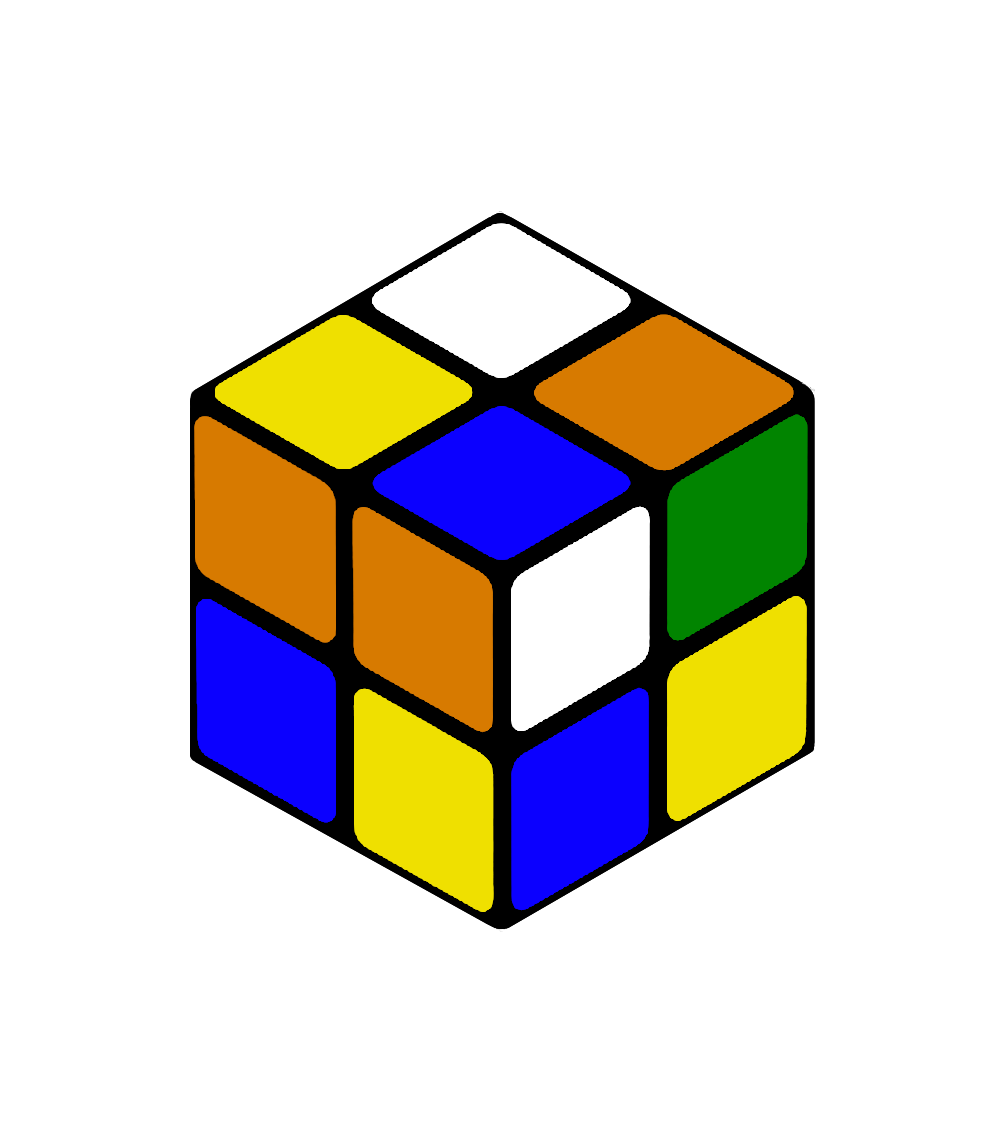
\includegraphics[scale=0.12]{LURFL1.png}
\caption{Würfel nach Zug $FUBRF^{-1}$ }
\label{Abbildung_LösungMensch0}
\end{figure}

Im ersten Schritt des menschlichen Ansatzes zum Lösen des Würfels sollen die Steine der oberen Ebene so angeordnet werden, dass die Farbflächen dort alle weiß sind und die vier oberen Steine in der richtigen Position zueinander sind. 
Für die Lösung der oberen Ebene muss $x_{1-4} = (0,0,0,0)$ gelten und die Steine der Ebene müssen an der richtigen Position zueinander sein.

Dafür sucht der Lösende Steine mit weißen Farbflächen und findet den weiß-orange-blauen Stein an der Position \textit{urf}. 
Mit dem Zug $F^{-1}$ findet der Stein seinen Platz in der oberen Ebene, mit der weißen Farbfläche oben. 
Nun ist $x_{1-4}''=(0,2,0,1)$. Der Würfel ist in Abbildung \ref{Abbildung_LösungMensch1} dargestellt: Es befinden sich nun zwei Steine der oberen Ebene richtig ausgerichtet an der richtigen Position -- der weiß-orange-blaue Stein und der weiß-rot-blaue Stein. Die neue Würfelkonfiguration ist dann $C'' $ $= C' \cdot F^{-1} $ $= ((\textit{ulb} \ \textit{urb} \ \textit{ulf} \ \textit{dlb} \ \textit{dlf} \ \textit{drb} \ \textit{urb}),$ $(0,2,0,1,1,2,2,1))$.

\begin{figure}[H]
\centering
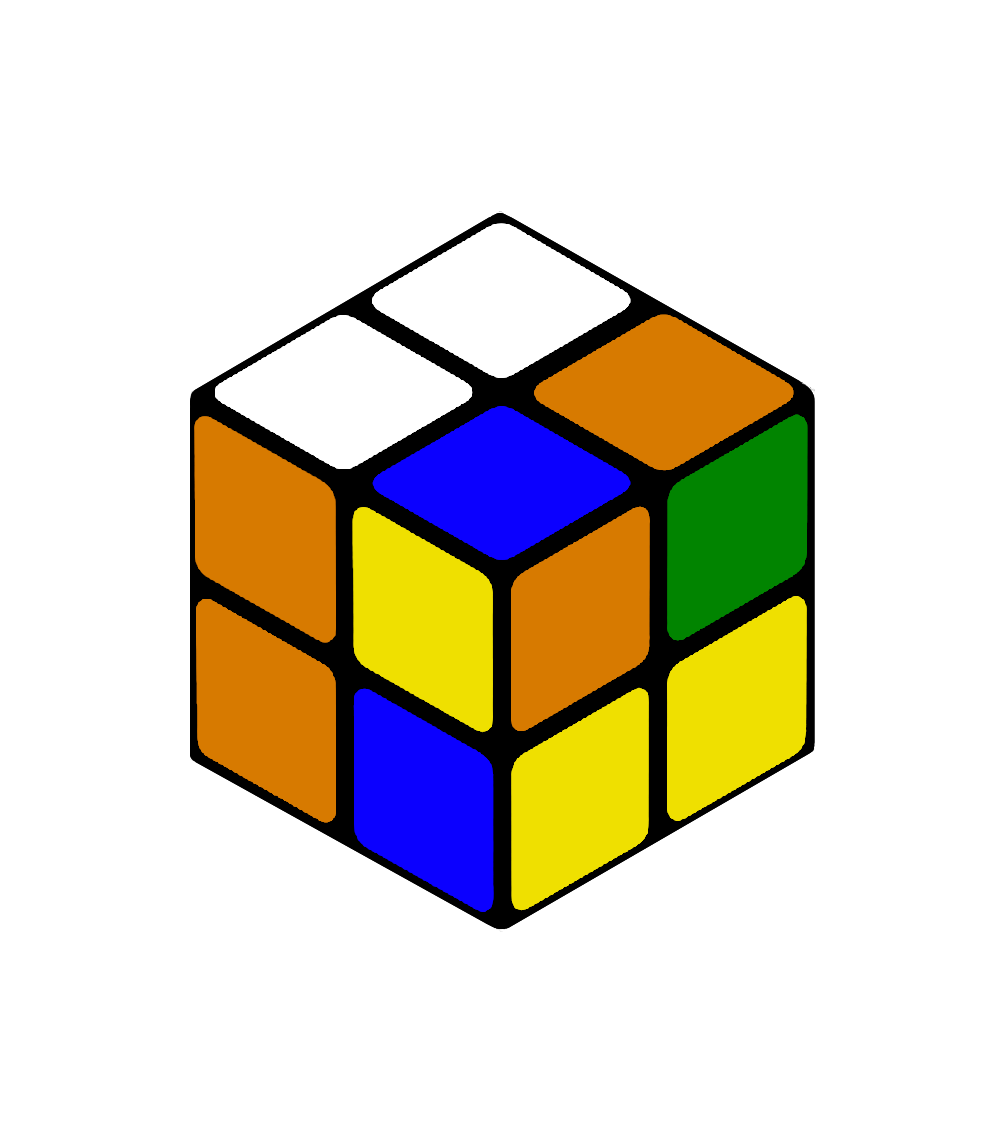
\includegraphics[scale=0.12]{0201.png}
\caption[Lösung von Mensch: Schritt 1]{Lösung von Mensch: Schritt 1}
\label{Abbildung_LösungMensch1}
\end{figure}

Der nächste Stein, der angeordnet wird, ist hier der weiß-grün-orange Stein. Er wird durch den Zug $R^{-1}$ in Position gebracht und findet seinen Platz neben dem weiß-orange-blauen Stein in der oberen Ebene (s. Abbildung \ref{Abbildung_LösungMensch2}). Die Würfelkonfiguration $C'''$ ist dann $C'' \cdot R^{-1} = (( \textit{ulb} \ \textit{urf} ) \ ( \textit{drb} \ \textit{drf} ) \ ( \textit{urb} \ \textit{ulf} \ \textit{dlb} \ \textit{dlf}),(0,1,0,0,2,0,1,2))$.
 
\begin{figure}[H]
\centering
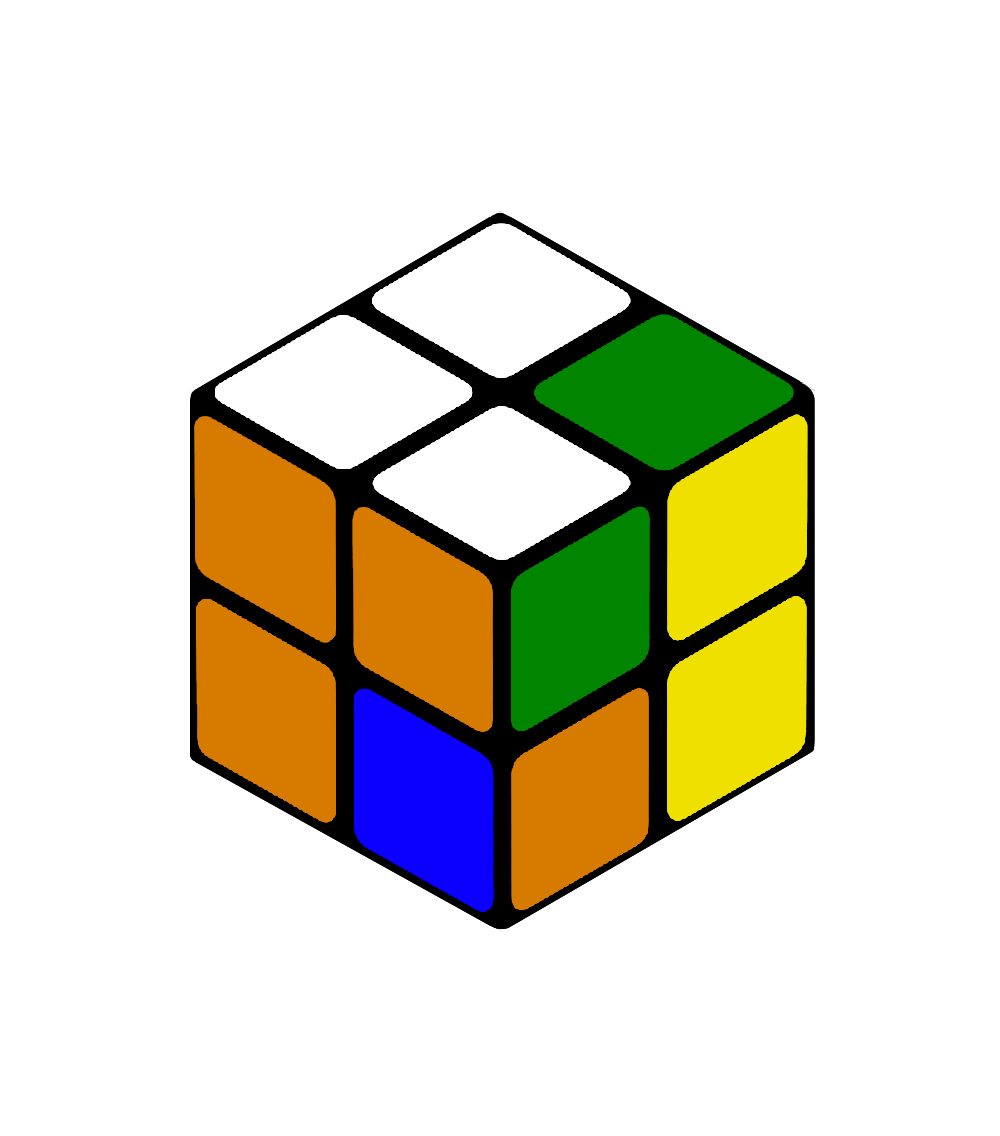
\includegraphics[scale=0.12]{menschSchritt2.png}
\caption[Lösung von Mensch: Schritt 2]{Lösung von Mensch: Schritt 2}
\label{Abbildung_LösungMensch2}
\end{figure}

Der letzte Stein mit weißer Farbfläche wird dann durch den Zug $RD^{-1}R^{-1}$ positioniert. Die obere Ebene ist nun gelöst und alle Steine mit weißen Farbflächen sind wie in der Startkonfiguration zueinander ausgerichtet. (s. Abbildung \ref{Abbildung_LösungMensch3}).
Die Würfelkonfiguration ist $C^{IV}=(( \textit{ulb} \ \textit{urf} ) \ ( \textit{urb} \ \textit{ulf} ) \ ( \textit{drb} \ \textit{drf} \ \textit{dlf} ),(0,0,0,0,2,0,1,0))$.

\begin{figure}[H]
\centering
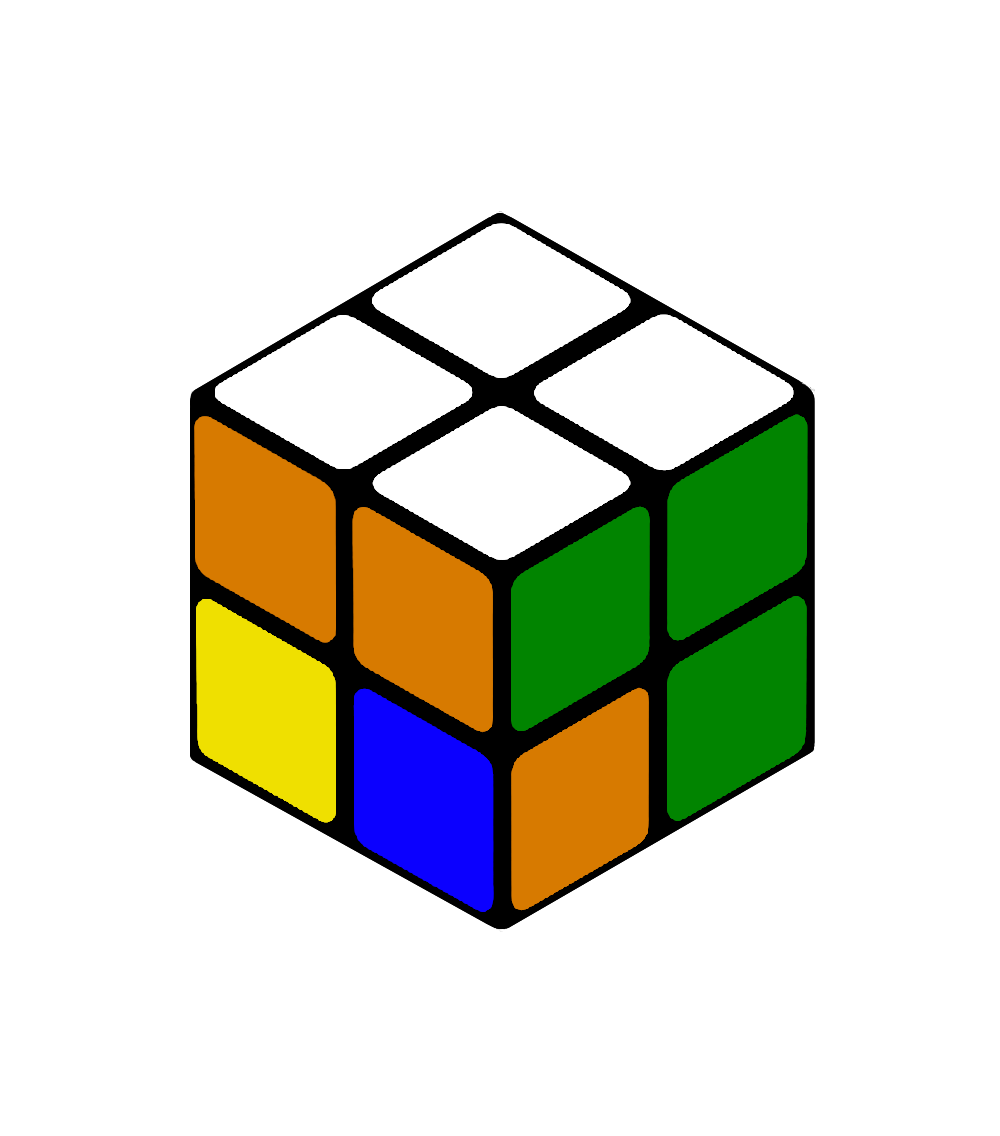
\includegraphics[scale=0.12]{menschSchritt3.png}
\caption[Lösung von Mensch: Schritt 3]{Lösung von Mensch: Schritt 3}
\label{Abbildung_LösungMensch3}
\end{figure} 

Für den nächsten Schritt rotiert der Mensch den Würfel, hier zweimal um die $y$-Achse (s. Abbildung \ref{Abbildung_LösungMensch4}). Die weiße Seite ist nun unten und zwei der vier gelben Farbflächen sind nach oben ausgerichtet. Dann ist die Würfelkonfiguration $C^V $ $= (( \textit{ulb} \ \textit{drb} \ \textit{urb} \ \textit{dlb} \ \textit{ulf} \ \textit{drf} ) \ ( \textit{urf} \ \textit{dlf} ),$ $(1,0,2,0,0,0,0,0))$. $C^V$ ist zu $C^{VI}$ äquivalent, da der Würfel nur rotiert wurde.

\begin{figure}[H]
\centering
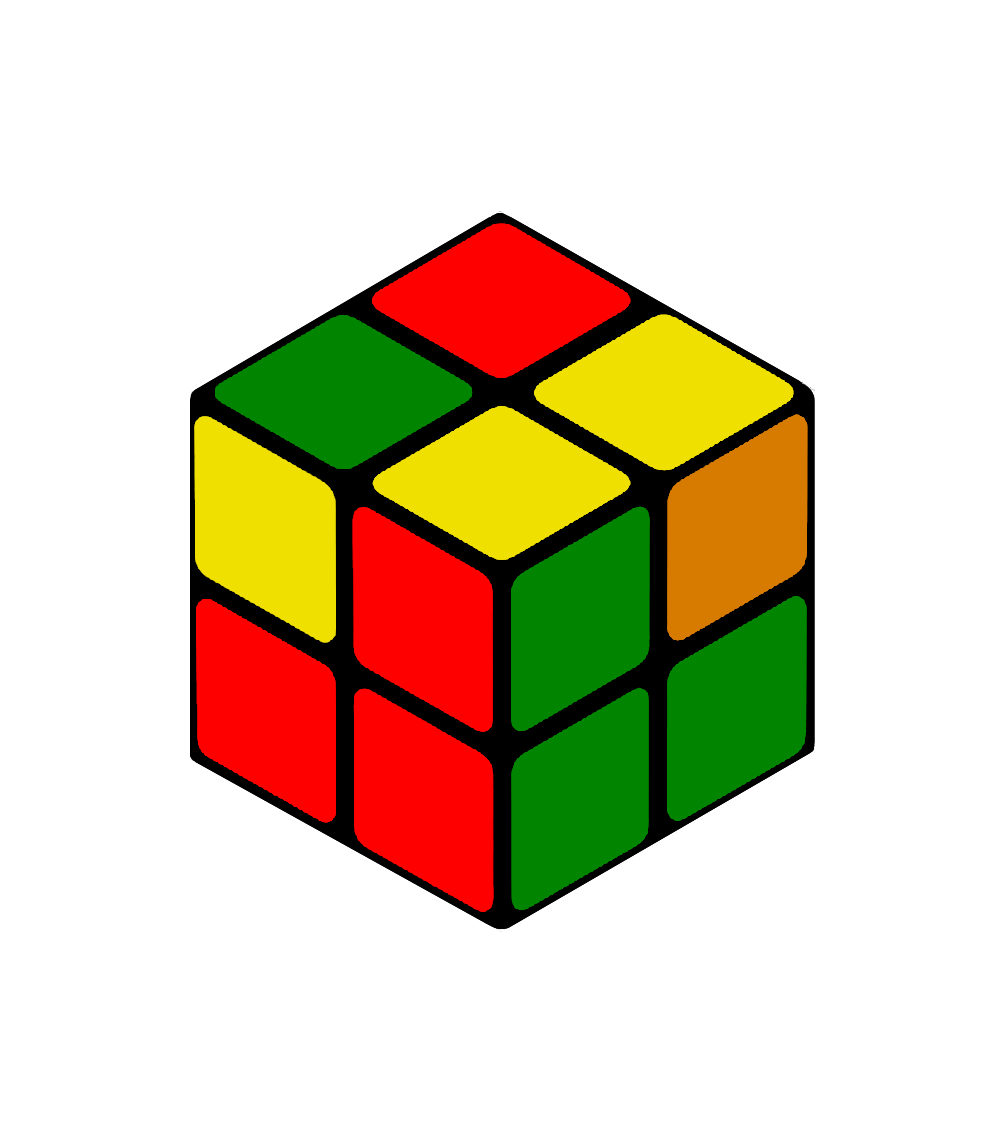
\includegraphics[scale=0.12]{menschSchritt4.png}
\caption[Lösung von Mensch: Schritt 4]{Lösung von Mensch: Schritt 4}
\label{Abbildung_LösungMensch4}
\end{figure} 

Dann führt der Lösende den Zug $RUR^{-1}U^{-1} \ R^{-1}FRF^{-1}$ aus \cite{RF2} und erhält einen gelösten Würfel, der falsch herum gehalten wird (s. Abbildung \ref{Abbildung_LösungMensch5}). 

\begin{figure}[H]
\centering
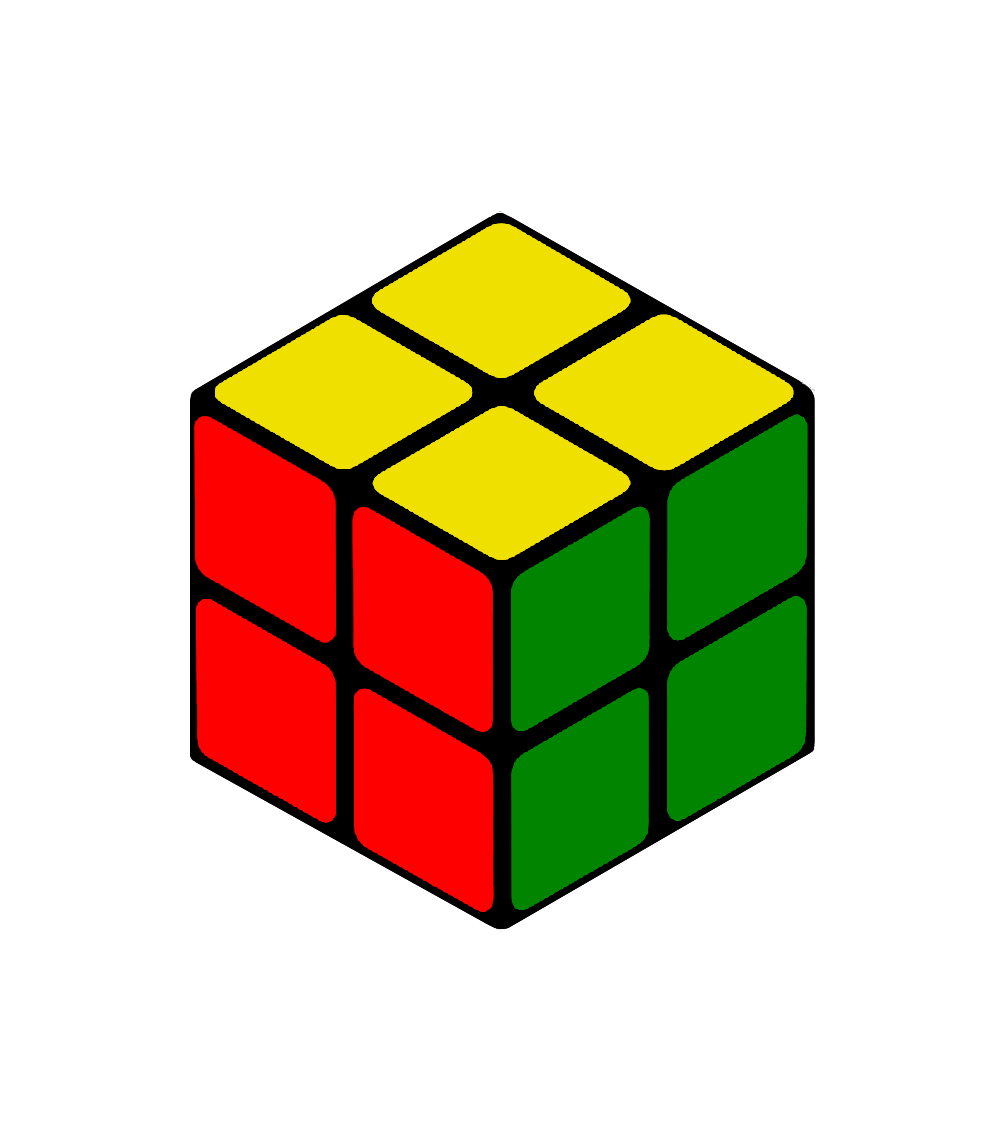
\includegraphics[scale=0.12]{menschSchritt5.png}
\caption[Lösung von Mensch: Schritt 5]{Gelöster \textit{Cube} mit weißer Seite unten}
\label{Abbildung_LösungMensch5}
\end{figure} 

Die Würfelkonfiguration ist $ C^{VI} = (( \textit{ulb} \ \textit{drb} ) \ ( \textit{urb} \ \textit{dlb} ) \ ( \textit{ulf} \ \textit{drf} ) \ ( \textit{urf} \ \textit{dlf} ), (0,0,0,0,0,0,0,0))$. Diese Konfiguration ist äquivalent zu der Konfiguration $(1,0)$.
Daher wird dieser Würfel nun noch zweimal um die $x$-Achse gedreht und befindet sich dann in der Konfiguration $C^{VII} =(1,0)$.

Der Mensch folgt beim Lösen des \textit{Cubes} bestimmten Kombinationen, die in verschiedenen Situtionen angewandt werden können.  
In diesem Fall hat der Mensch $13$ Ebenendrehungen durchgeführt, während das Verdrehen lediglich $5$ Ebenenrotationen benötigte. Der Mensch hat folglich nicht den kürzesten Weg gewählt, aber dafür einen Weg, den er bei verschiedenen Würfelkonfiguratonen anpassen und verwenden kann. 
Wenn die Verdrehung des Würfels invertiert wird ($(FUBRF^{-1})^{-1}$), ergibt das die Kombination $FR^{-1}B^{-1}U^{-1}F^{-1}$, um den Würfel zu lösen.
Es stellt sich die Frage, wie viele Ebenendrehungen für den optimalen Lösungsweg maximal erforderlich sein können. Diese Zahl wird auch \textit{God's Number} genannt. 

\subsubsection*{God's Number}
Im Folgenden werden die \textit{God's Number}, \textit{Quarter-Turn} Metrik und \textit{Half-Turn} Metrik kurz beschrieben.
Bei einer Ebenendrehung werden die Ebenen um $90^\circ$ gedreht. Eine Ebenendrehung um $180^\circ$ wird als zwei Vierteldrehungen gewertet. Das wird \textit{Quarter-Turn} Metrik genannt. Es gibt noch andere Metriken, wie z. B. die \textit{Half-Turn} Metrik, bei der eine Drehung der Ebene sowohl um $90^\circ$ als auch um $180^\circ$ als eine Drehung gezählt wird \cite{TR}.
Nach der \textit{Quarter-Turn} Metrik gerechnet ist die \textit{God's Number} des \Ttwo Würfels $14$ \cite{DJ}. In der \textit{Half-Turn} Metrik ist sie $11$ \cite{RMG}.
Ein Konzept zum Finden der optimalen Lösung mithilfe der \textit{Quarter-Turn} Metrik wird in Abschnitt \ref{Abschnitt_MinLösung} beschrieben.


%
%
%
%
%
%
%
%
%
%=======================================================================================================
%
%
%
%
%
%
%
%
%
%
\subsection{Muster}

Dieser Abschnitt wurde von dem Abschnitt \textit{Pretty Patterns} in Tom Davis' \textit{Group Theory via Rubik's Cube} inspiriert \cite{TD}.
Dort werden acht \textit{hübsche} Muster des \Tthree Würfels gezeigt. In diesem Abschnitt werden vier Muster des \Ttwo Würfels gezeigt und die dazugehörigen Algorithmen von der Startkonfiguration ausgehend beschrieben. Diese vier Muster sind in Abbildung \ref{Abbildung_Muster} dargestellt.
Außerdem wird die Konfiguration der Würfels angegeben.

\begin{figure}[h]
\centering
\begin{tabular}{cc}
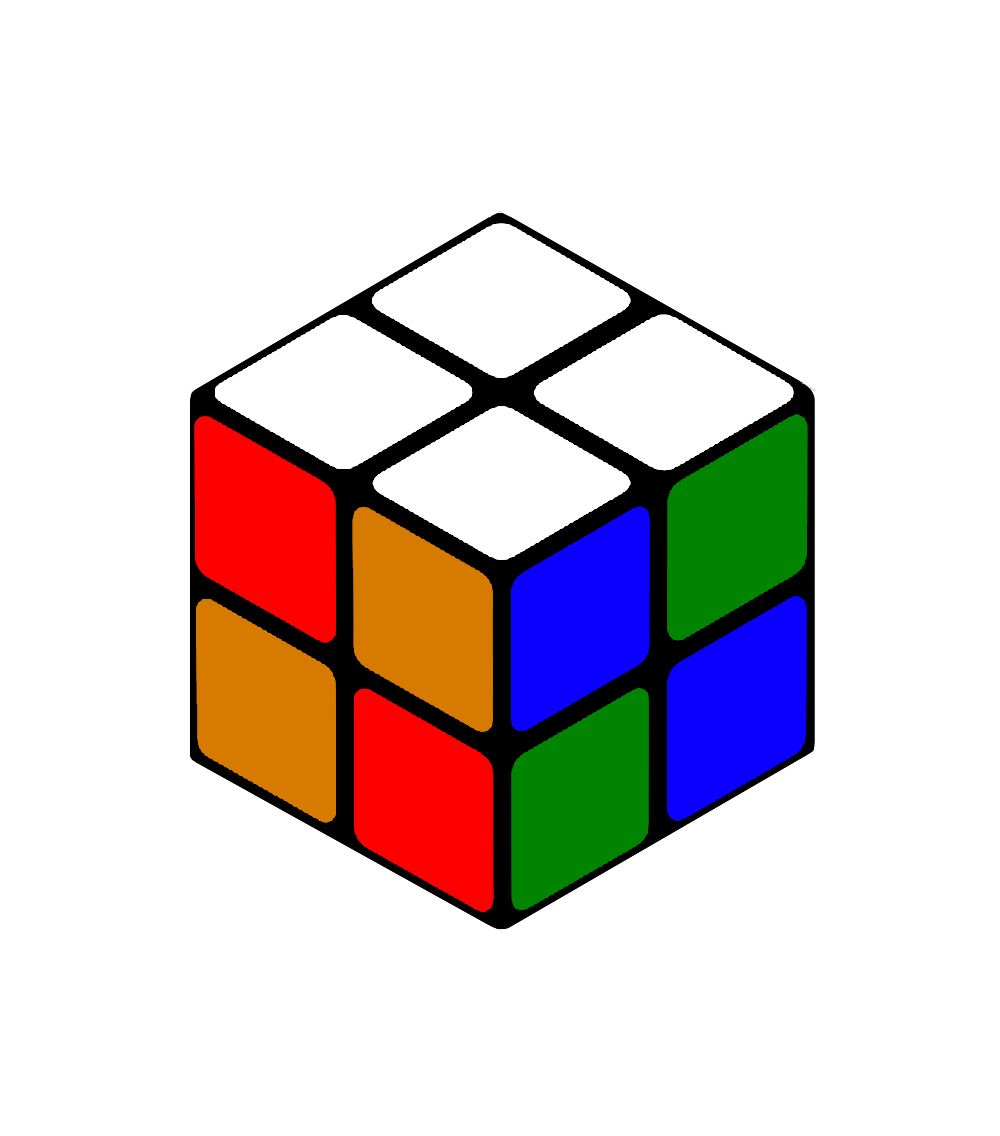
\includegraphics[scale=0.1]{RRFFRRUU.png} &  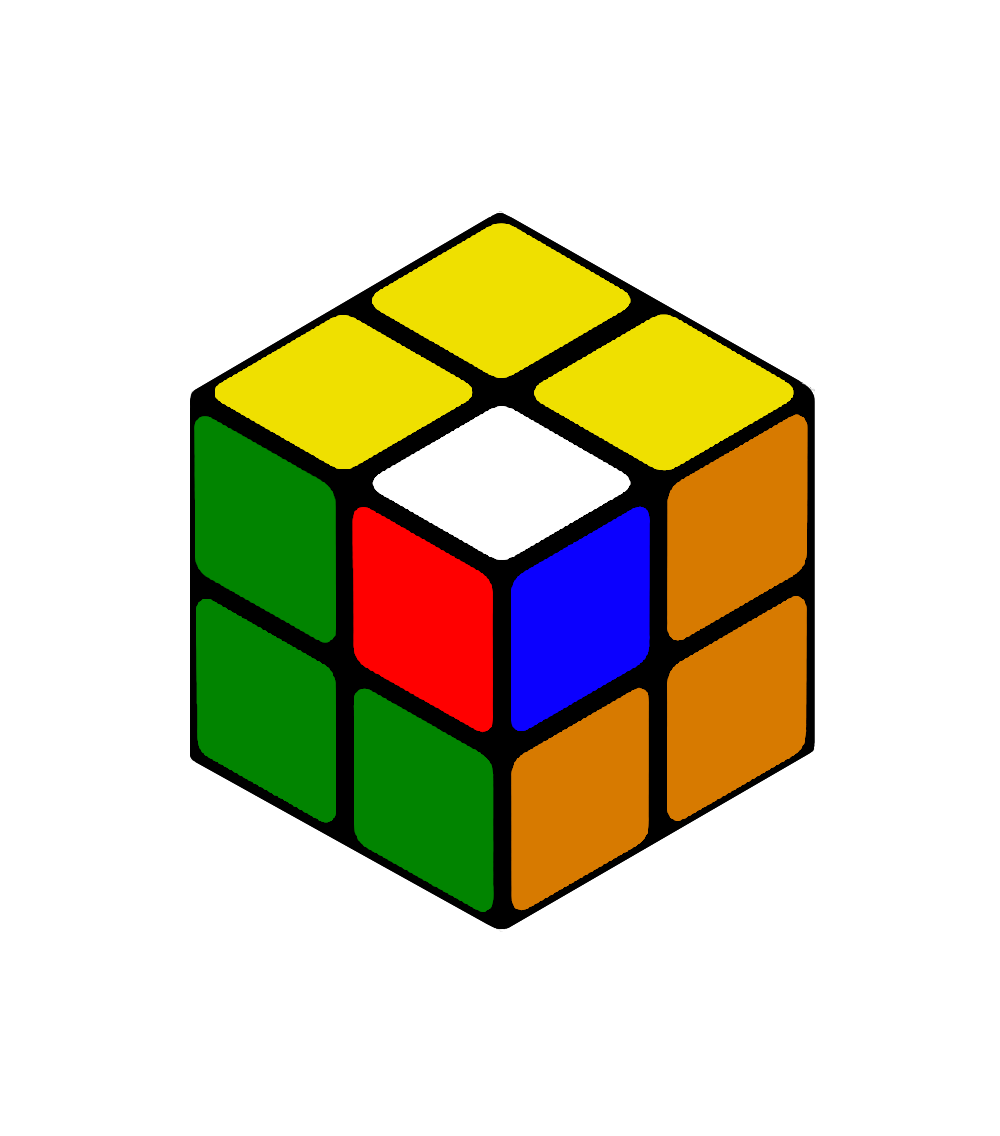
\includegraphics[scale=0.1]{CubeInCube.png} \\
Muster 1 & Muster 2 \\
$RR \ FF \, RR \ UU$ &  $R \ F \, U^{-1} \, RR \ U \, F^{-1} \, R \ U \, FF \, RR$ \\
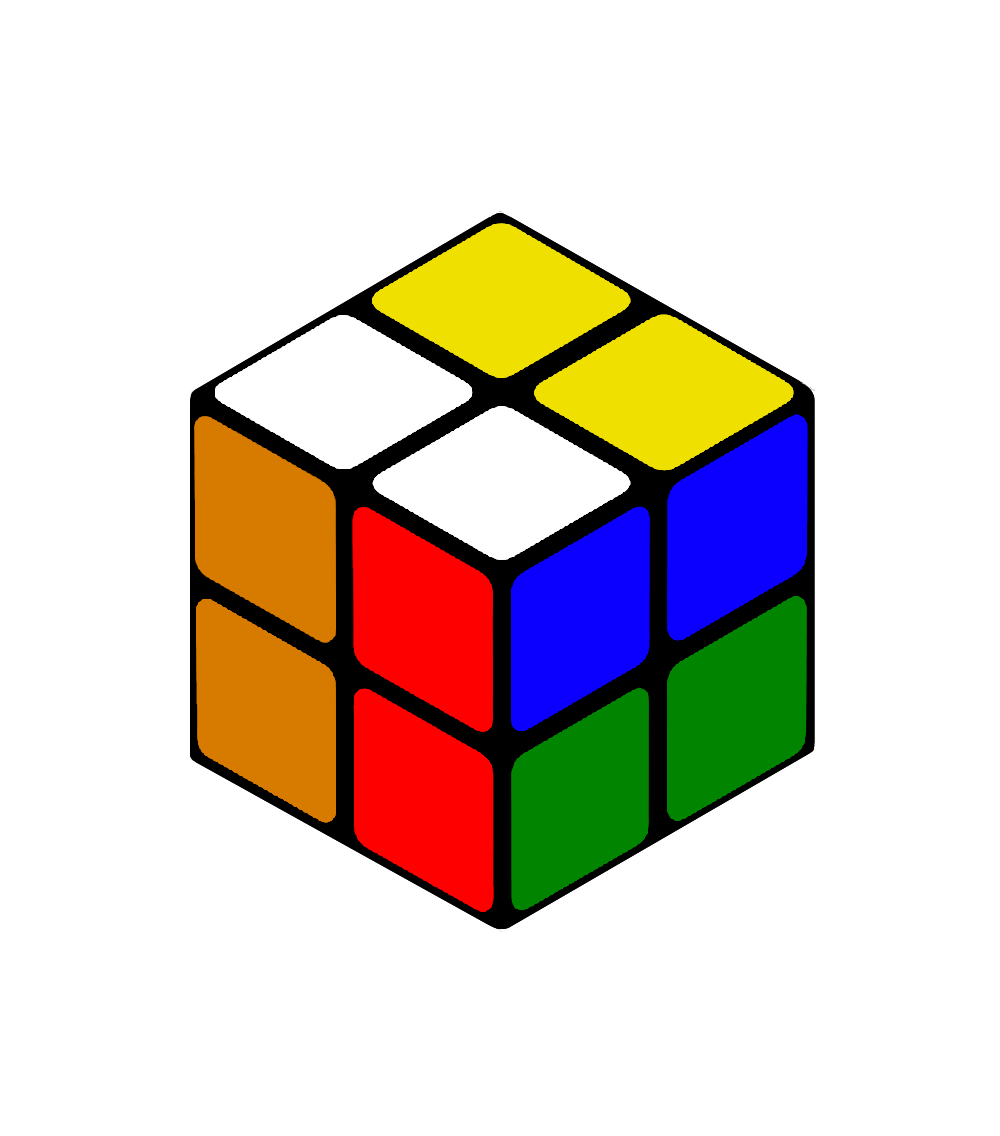
\includegraphics[scale=0.1]{UUFFRRUU.png} &  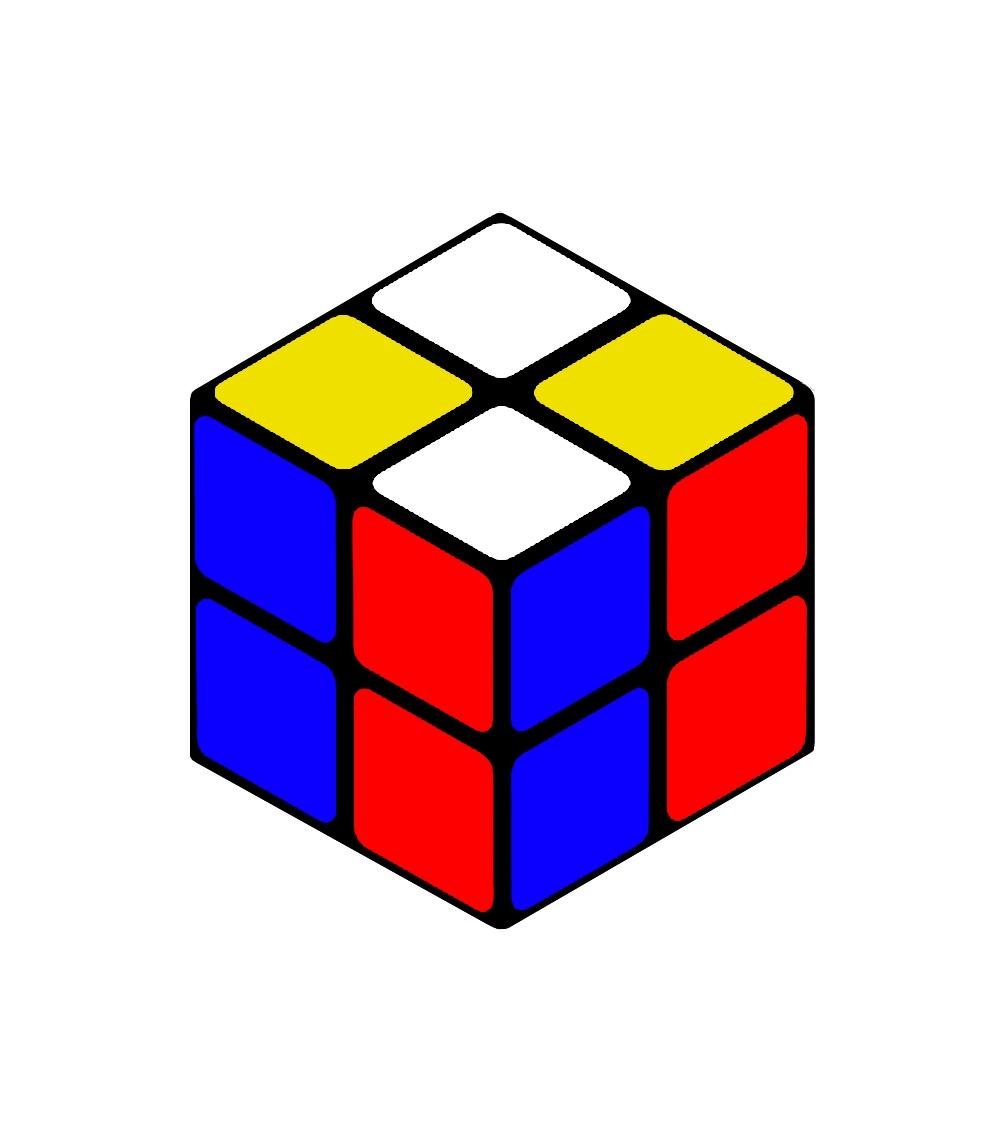
\includegraphics[scale=0.1]{UFFUURRU.png} \\
Muster 3 & Muster 4 \\
$UU \, FF \, RR \ UU$ &  $U \, FF \, UU \, RR \ U$ \\
\end{tabular}

\caption{Muster des \Ttwo Würfels}
\label{Abbildung_Muster}
\end{figure}

Muster 1 lässt die weiße und gelbe Seite unverändert und bildet ein Karomuster auf den anderen vier Seiten. Dabei werden die Farbpaare rot-orange und grün-blau zusammen im  Karomuster angeordnet. Die Konfiguration des Würfels ist dann $C = ((\textit{ulb} \ \textit{urf} ) \ ( \textit{drb} \ \textit{dlf} ),(0,0,0,0,0,0,0,0))$.

Muster 2 hat einen \textit{Würfel im Würfel}. Dabei werden zwei Steine getauscht, die keine gemeinsame Farbfläche haben. Der Würfel befindet sich dann in der Konfiguration $C = (( ulb \ drf ) \ ( ulf \ dlf ) \ ( drb \ urb ),(0,0,0,0,0,0,0,0))$

Muster 3 zeigt abwechselnd Quer- und Längsstreifen auf den verschiedenen Seiten. Die Konfiguration des Würfels ist dann $C = (( \textit{ulb} \ \textit{dlf} \ \textit{drb} ) \ ( \textit{urb} \ \textit{ulf} \ \textit{drf} )),(0,0,0,0,0,0,0,0))$.

Muster 4 ordnet die Farben wie vier Säulen an. Die weiße und die gelbe Seite sind dabei kariert, die anderen Seiten gestreift. Die Konfiguration des Würfels ist dann $C = ( (\textit{urb} \ \textit{dlf} ) \ ( \textit{ulf} \ \textit{drb}  ) ),(0,0,0,0,0,0,0,0))$.


Diese Muster sind in den meisten Fällen zwar keine üblichen Lösungsalgorithmen, sollten aber in dieser Arbeit auch nicht unerwähnt bleiben.

%
%
%
%
%
%
%
%
%
%=======================================================================================================
%
%
%
%
%
%
%
%
%
%
\subsection{Schraubendrehermethode}

Die Methode, die oft als simpelste Methode zum Lösen von Zauberwürfeln beschrieben wird, ist die Schraubendrehermethode.
Bei den üblichen \Ttwo Würfel ist auf einer oder mehreren Seiten in der Mitte zwischen den Steinen eine Schraube zu sehen (s. links in Abbildung \ref{Abbildung_Schraubendrehermethode}).
Um den Würfel auseinander zu bauen, muss diese Schraube gelockert werden. Daraufhin kännen die Steine ohne Probleme abgenommen werden. 
Dann werden die Steine neu arrangiert und der Würfel kann in der gelösten Konfiguration wieder zusammen gebaut werden.

\begin{figure}[H]
\centering
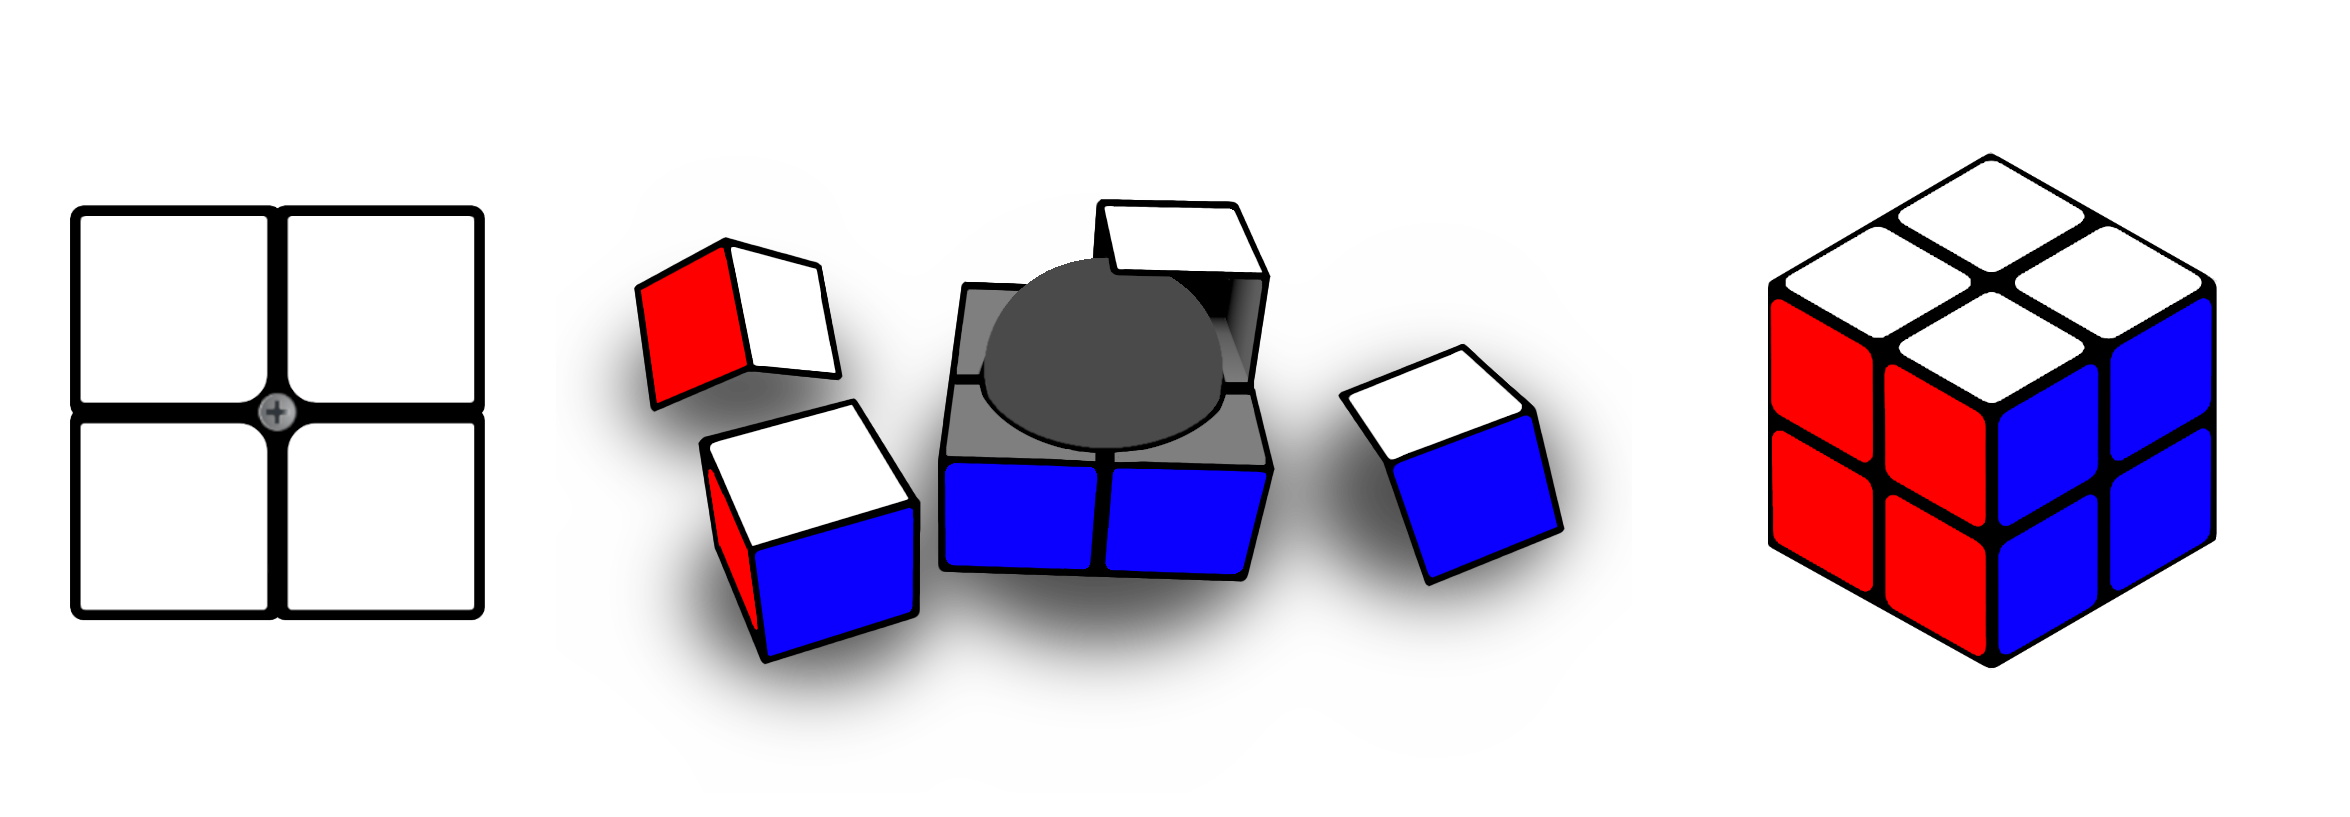
\includegraphics[scale=0.2]{schraube_m.png}
\caption{Lösung durch Schraubendrehermethode}
\label{Abbildung_Schraubendrehermethode}
\end{figure}

Ob das wirklich die simpelste Methode ist, liegt wohl im Auge des Betrachters und unter Berücksichtigung der Tatsache, dass der Weltrekord des \Ttwo Würfels mit der Methode des algorithmischen, händischen Lösens bei $0,49$ Sekunden liegt \cite{rekord}, ist die Schraubendrehermethode wohl kaum die schnellste Methode.

%
%
%
%
%
%
%
%
%
%=======================================================================================================
%
%
%
%
%
%
%
%
%
%
\subsection{Algorithmen für die erste Ebene}
\label{Abschnitt_AlgorithmenErsteEbene}

In diesem Abschnitt werden Algorithmen zum Lösen der ersten Ebene mit der Fridrich-Methode beschrieben. Bei dieser Methode werden im ersten Schritt die vier Steine der oberen Ebene richtig ausgerichtet und richtig zueinander angeordet. Die Vorgehensweise dieser Methode wurde bereits in Abschnitt \ref{Abschnitt_Lösungsansätze} beschrieben. 

Die Fridrich-Methode ist ein Lösungsansatz für den \Tthree Würfel, der auf den \Ttwo übertragen werden kann.
Da der \Ttwo im Gegensatz zum \Tthree Würfel keine Mittelsteine hat, kann ein Eckstein als richtig angenommen werden, da der Würfel lediglich rotiert werden muss, um eine weiße Farbfläche zu finden.
In diesen Beschreibungen wird sich an die Konvention gehalten, mit der weißen Seite zu beginnen. Es kann aber ebenso mit jeder anderen Seite des Würfels begonnen werden.
Der \Tthree \textit{Cube} muss entsprechend der Mittelsteine ausgerichtet werden und so ist vorbestimmt, welche Seite die weiße Seite wird. Die weiße Seite muss den weißen Mittelstein enthalten. 
Bei dem \Ttwo \textit{Cube} kann mit jeder beliebigen Seite begonnen werden. Wenn mit einer bestimmten Seite als Oberseite begonnen werden soll, die noch keine weiße Farbfläche hat, so kann die Farbfläche durch maximal zwei Ebenendrehungen an diese Seite gebracht werden.

In Abbildung \ref{Abbildung_ErsterEckstein} wird der erste Eckstein der oberen Ebene positioniert. Das kann dort entweder durch den Zug $R$ oder einer Rotation um die $y$-Achse passieren.

\begin{figure}[H]
\centering
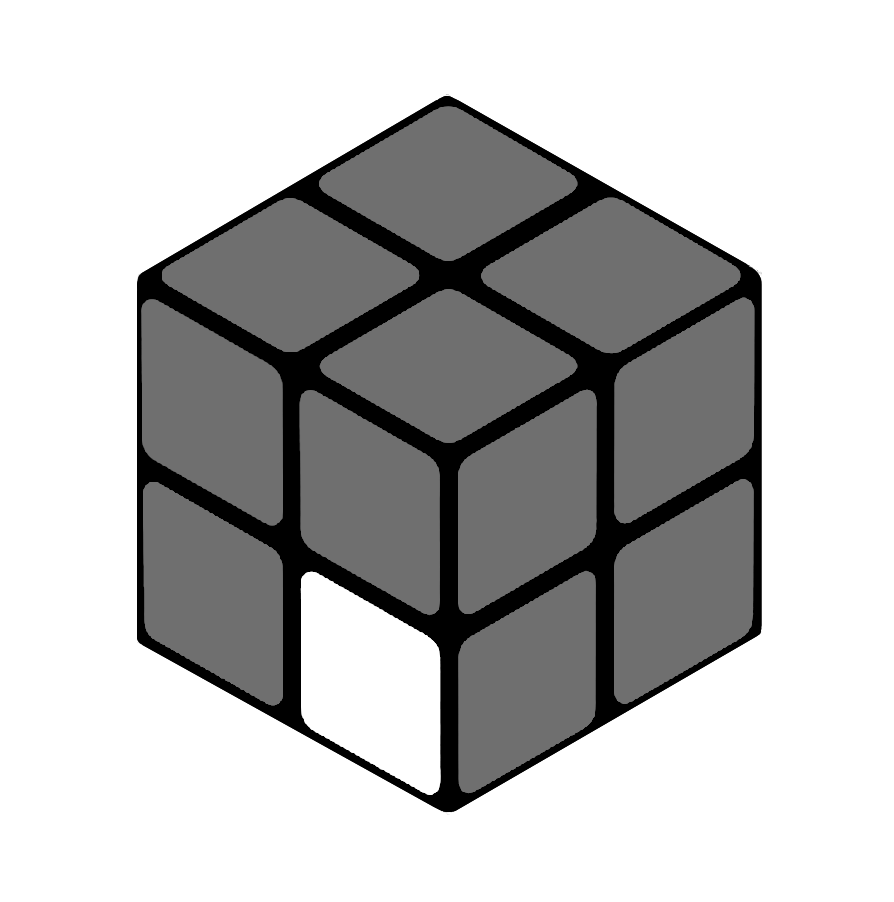
\includegraphics[scale=0.1]{e1_s1_s1.png}
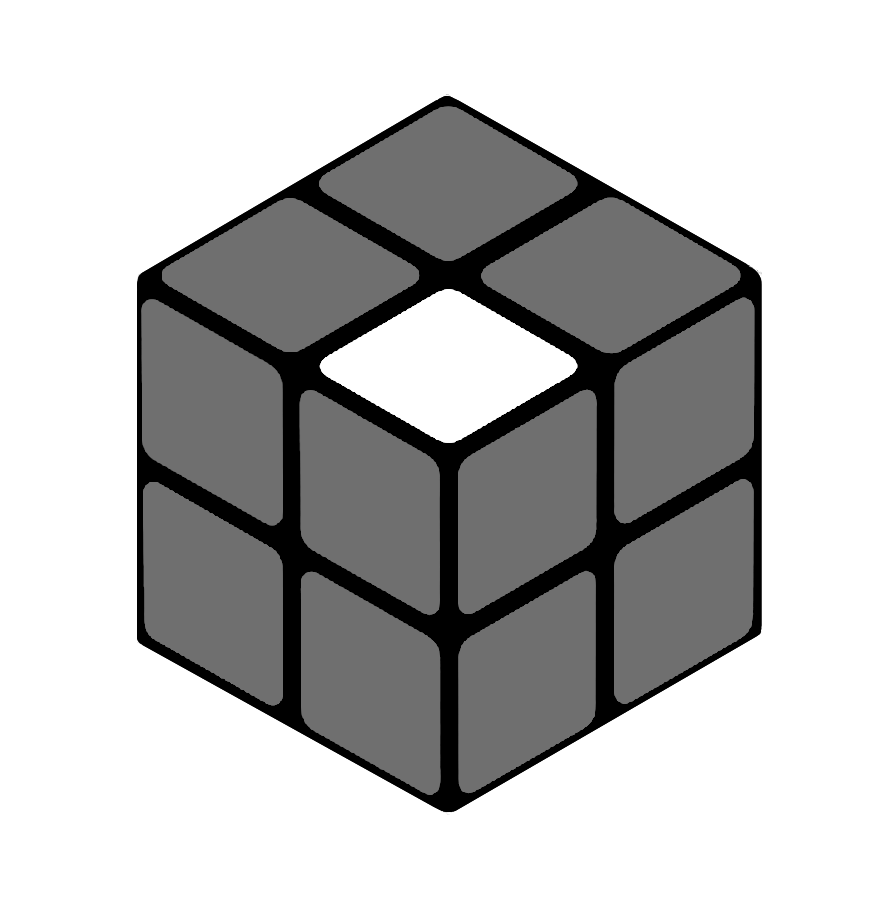
\includegraphics[scale=0.1]{e1_s1_s2.png}
\caption{Ersten Eckstein positionieren}
\label{Abbildung_ErsterEckstein}
\end{figure}

Der zweite Stein kann dann hinzugefügt werden.
Für diesen Algorithmus muss sich die weiße Farbfläche des zweiten Steins seitlich an der unteren Ebene befinden. Optimalerweise befindet sich der Stein schon zufällig an der gewünschten, korrekten Position.
Ansonsten wird $D$ ausgeführt, bis der Stein sich unter seiner Zielposition befindet und er wird mit $L, R, F$ oder $R$ neben den bereits vorhandenen ersten Eckstein gedreht. Das ist auch in Abbildung \ref{Abbildung_ZweiterEckstein} zu sehen.

\begin{figure}[H]
\centering
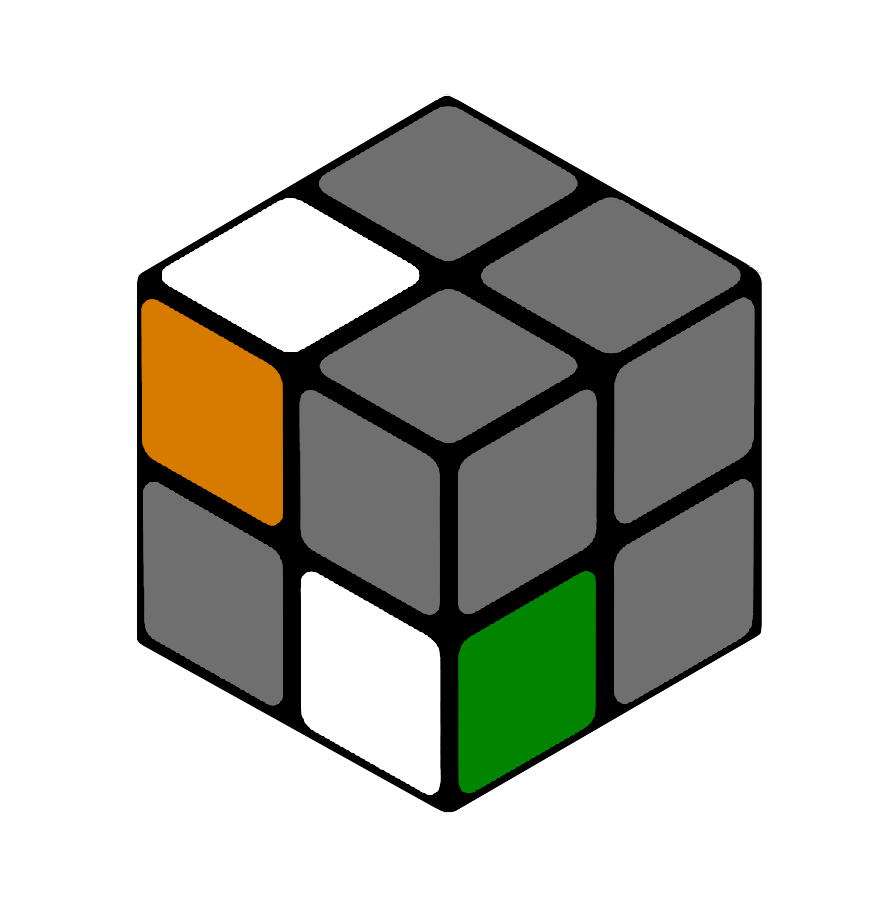
\includegraphics[scale=0.1]{e1_s2_s1.png}
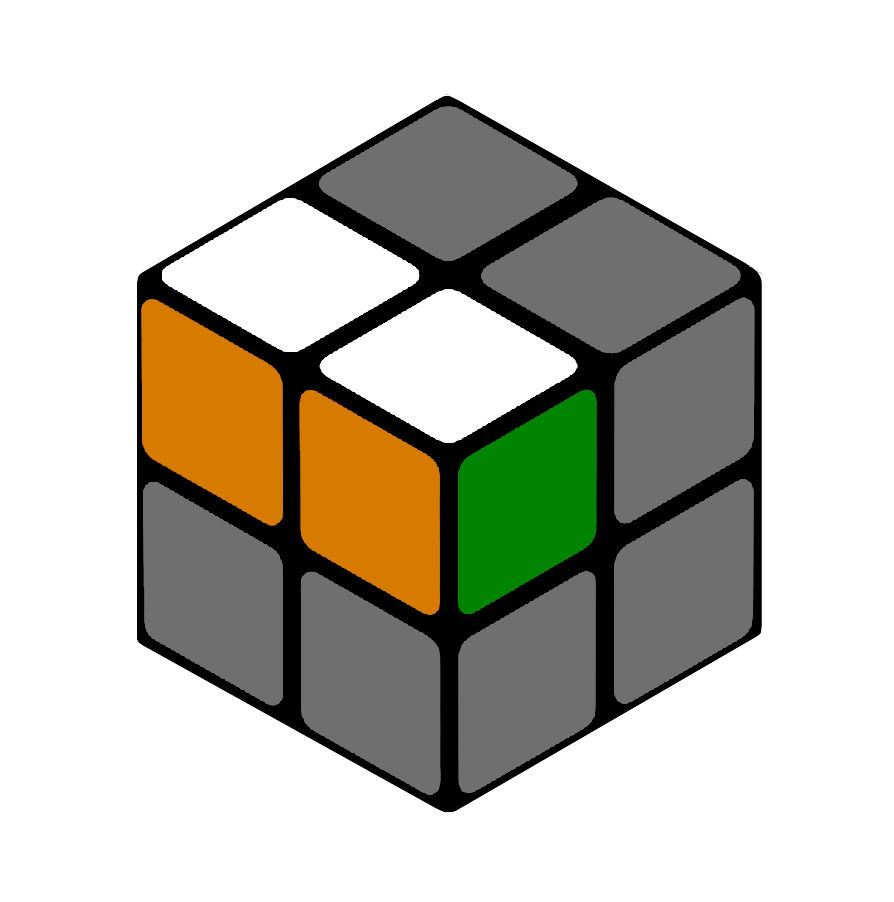
\includegraphics[scale=0.1]{e1_s2_s2.png}
\caption{Zweiten Eckstein positionieren}
\label{Abbildung_ZweiterEckstein}
\end{figure}

Dort sind auch orange und grüne Farbflächen abgebildet. Das gilt analog für die anderen benachbarten Farbflächen. Zu beachten ist, dass die beiden Farbflächen einer Seite auch die gleiche Farbe haben.

Sollte sich die weiße Farbfläche der Ecke unten am Würfel befinden, so kann sie falsch herum ausgerichtet mit der Technik aus Abbildung \ref{Abbildung_ZweiterEckstein} an die Position gesetzt werden. Dann befindet sich die weiße Farbfläche in der oberen Ebene, aber falsch herum ausgerichtet. Wenn das der Fall ist, kann der Stein mit einem der Züge $L, R, F$ oder $B$ herausgedreht werden und mit $U$ in die untere Ebene geschoben werden. Dieser Vorgang ist auch in Abbildung \ref{Abbildung_ZweiterEckstein2} zu sehen. Danach wird er mit der oben beschriebenen Technik richtig ausgerichtet und positioniert eingefügt (s. Abbildung \ref{Abbildung_ZweiterEckstein}). 

\begin{figure}[H]
\centering
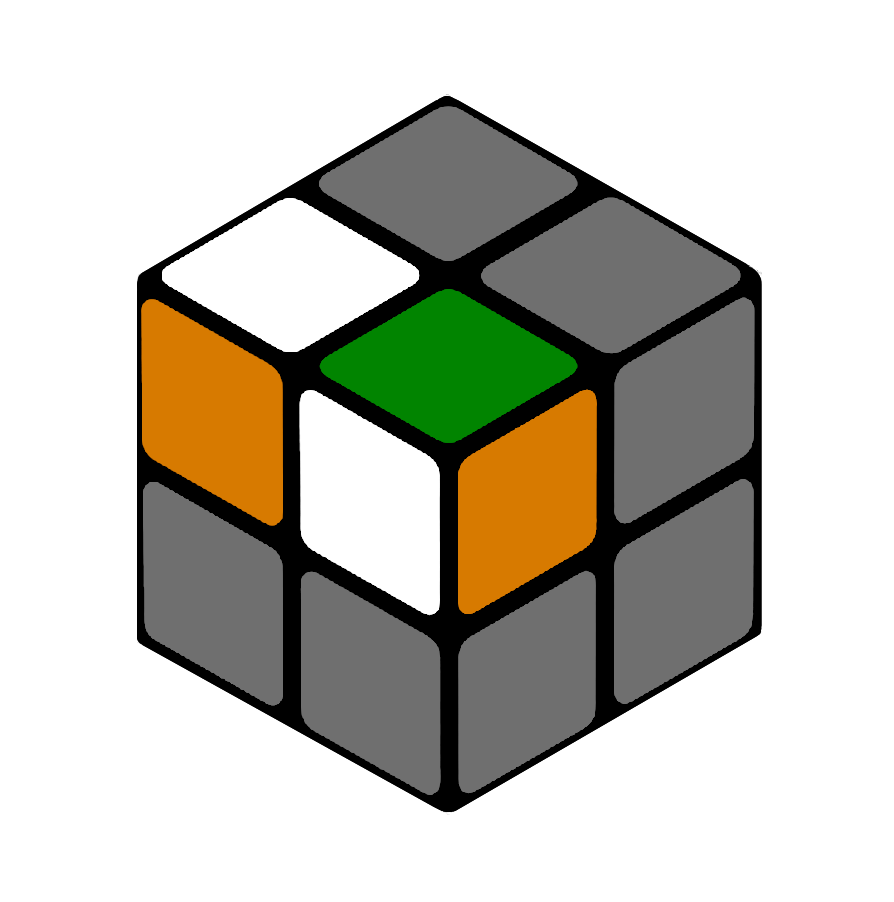
\includegraphics[scale=0.1]{e1_s2_s1_s.png}
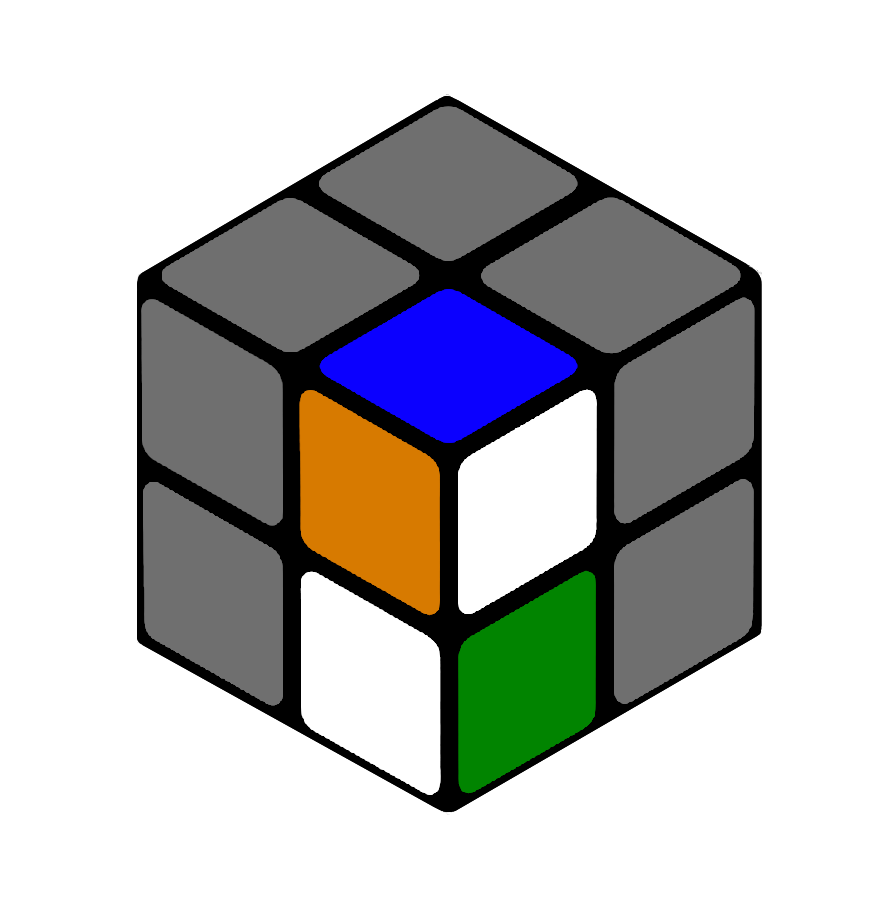
\includegraphics[scale=0.1]{e1_s2_s2_s.png}
\includegraphics[scale=0.1]{e1_s2_s3_s.png}
\includegraphics[scale=0.1]{e1_s2_s4_s.png}
\caption{Zweiter Eckstein: Sonderfall}
\label{Abbildung_ZweiterEckstein2}
\end{figure}

Dieletzten beide Steine der ersten Ebene lassen sich mit der oben genannten Technik ebenfalls positionieren. Die obere Ebene ist dann gelöst. Die Vektoreinträge $x_{1-4}$ sind dann $(0,0,0,0)$.
Bei dem \Ttwo Würfel entspricht das Lösen der oberen Ebene sogar schon der Hälfte des Würfels. Die Algorithmen für die zweite Ebene sind in Abschnitt \ref{Abschnitt_AlgorithmenZweiteEbene} zu finden.



%
%
%
%
%
%
%
%
%
%=======================================================================================================
%
%
%
%
%
%
%
%
%
%
\subsection{Algorithmen für die zweite Ebene}
\label{Abschnitt_AlgorithmenZweiteEbene}

Beim Lösen der zweiten Ebene muss beachtet werden, die erste Ebene nicht wieder zu verdrehen. Deshalb sind die Algorithmen hier länger, um spezifische Steine zu bewegen.
In Abbildung \ref{Abbildung_GelösteObereEbene} ist die obere Ebene des Würfels gelöst. 

\begin{figure}[H]
\centering
\includegraphics[scale=0.1]{ebene.png}
\caption{Würfel mit gelöster oberer Ebene}
\label{Abbildung_GelösteObereEbene}
\end{figure}


Ein Mensch dreht den Würfel zum Lösen der zweiten Ebene meistens um, damit die entsprechenden Steine sichtbar sind. Der Anschaulichkeit halber wird das hier auch gemacht.

Zuerst werden nun alle Steine der zweiten Ebene richtig ausgerichtet, so dass die obere Seite des Würfels ausschließlich gelbe Farbflächen zeigt. Der Vektor $x$ ist dann $0$. Danach werden die Steine getauscht, bis sie richtig angeordnet sind. Dann ist die Permutationsfunktion $\sigma = 1$.

Da es viele mögliche Würfelkonfigurationen und Algorithmen zur Lösung dieser gibt, werden die möglichen Steinpositionen und Algorithmen in einer Tabelle aufgeführt. Die Algorithmen führen alle zu einer Würfelkonfiguration, bei der die untere (bereits gelöste) Ebene unverändert bleibt und die obere Seite ausschließlich gelbe Farbflächen zeigt.
Viele dieser Algorithmen enthalten $(R U R^{-1} U^{-1})$, was hier als Kommutator $[ R,U ]$ geschrieben wird. Kommutatoren der Würfelzüge wurden in Abschnitt \ref{Abschnitt_Kommutatoren8} behandelt.

\begin{center}
\begin{tabular}{m{4cm} m{6cm}}
\toprule
Ausgangsposition & Algorithmus  \\
\midrule
\includegraphics[scale=0.08]{TOPVIEW1.png} & $F \ [ R,U ] \  [ R,U ] \  [ R,U ] \ F^{-1}$ \\
\includegraphics[scale=0.08]{TOPVIEW2.png} & $F \ [ R,U ] \  [ R,U ] \ F^{-1}$ \\
\includegraphics[scale=0.08]{TOPVIEW3_1.png} & $R \ U \ R^{-1} \ U \ R \ UU \ R^{-1}$ \\
\includegraphics[scale=0.08]{TOPVIEW3_2.png} & $L^{-1} \ U^{-1} L \ U^{-1} \ L^{-1} \ UU \ L$ \\
\includegraphics[scale=0.08]{TOPVIEW4.png} & $F \ [ R,U ] \ F^{-1}$ \\
\includegraphics[scale=0.08]{TOPVIEW5.png} & $[ R,U ] \ [R^{-1}, F]$ \\
\bottomrule
\end{tabular}
\end{center}

\begin{center}
\begin{tabular}{m{4cm} m{6cm}}
\toprule
Ausgangsposition & Algorithmus  \\
\midrule

\includegraphics[scale=0.08]{TOPVIEW6.png} & $F^{-1} \ [ R,U ]\ L^{-1} \ U \ L$ \\
\bottomrule
\end{tabular}
\end{center}


Die obere Seite des Würfels zeigt nach dem Ausführen dieser Algorithmen auf die entsprechenden Ausgangspositionen ausschließlich gelbe Farbflächen. Die Ausrichtung der Steine ist dann bereits richtig und der Vektor $x$ somit $(0,0,0,0,0,0,0,0)$. Wenn alle Steine der zweiten Ebene dann bereits richtig zueinander angeordnet sind, muss die Ebene eventuell mit $U$, $U^{-1}$ oder $UU$ richtig zur ersten Ebene ausgerichtet werden.  Ansonsten werden die Steinpositionen getauscht, bis sie richtig angeordnet sind.

Zum Vertauschen der Steine untereinander, ohne die Ausrichtung zu verändern, gibt es verschiedene Algorithmen. Diese Algorithmen werden im Folgenden in einer Liste aufgeführt. Die Pfeile zeigen an, welche Steine beim Ausführen der Algorithmen an welche Würfelposition gelangen.

\begin{center}
\begin{tabular}{m{4cm} m{8cm}}
\toprule
Steinpermutation & Algorithmus  \\
\midrule
\includegraphics[scale=0.08]{corners1.png}  & $F \ R \ U^{-1} \ [R^{-1}, U^{-1}] \ R^{-1} \ F^{-1}  \ [R, U]   [R^{-1}, F]$ \\
\includegraphics[scale=0.08]{corners2.png}   & $[R,U] \  R^{-1} \ F \ RR \   U^{-1} \ [R^{-1}, U^{-1}] \ R^{-1} \  F^{-1})$ \\
\includegraphics[scale=0.08]{corners3.png}   & $R \ B^{-1} \ R \ FF \ R^{-1} \ B \ R \ FF \ RR $ \\
\bottomrule
\end{tabular}
\end{center}
%
%\begin{center}
%\begin{tabular}{m{4cm} m{8cm}}
%\toprule
%Steinpermutation & Algorithmus  \\
%\midrule
%
%\bottomrule
%\end{tabular}
%\end{center}

Nach dem Ausführen der passenden Algorithmen sind beide Ebenen gelöst. Eventuell müssen die beiden Ebenen noch durch $U$, $U^{-1}$ oder $UU$ richtig zueinander ausgerichtet werden. Dann befindet sich der Würfel im gelösten Zustand und die Würfelkonfiguration ist somit $(1,0)$.

Mit den Algorithmen aus dieser Anleitung kann jede valide Konfiguration eines \Ttwo Würfels in die Startkonfiguration $(1,0)$ überführt werden. Der beschriebene Ansatz ist die Fridrich-Methode.

%
%
%
%
%
%
%
%
%
%
%=======================================================================================================
%
%
%
%
%
%
%
%
%
%
\newpage

\section{Minimale Gruppe}
\label{Kapitel_MinUntergruppe}

In diesem Kapitel wird die Gruppe des \Ttwo Würfels mit minimalen Zügen realisiert. Die Gruppe des $(\Gtwo, \circ)$ ist eine vollständige Abbildung des \Ttwo Würfels -- sie ist aber nicht minimal. Solch eine minimale Abbildung wird in diesem Kapitel definiert. Diese minimale Abbildung ist eine Untergruppe von $(\Gtwo, \circ)$.
Die Untergruppe der minimalen Abbildung des \Ttwo Würfels wird $(G_{min}, \circ)$ genannt. Die Menge $G_{min}$ enthält die Äquivalenzklassen der minmalen Züge des Würfels.
Die Menge der minimalen Grundzüge erzeugt die Untergruppe $(G_{min}, \circ)$.

%
%
%
%
%
%
%
%
%
%
%=======================================================================================================
%
%
%
%
%
%
%
%
%
%
\subsection{Minimale Grundzüge}
\label{Abschnitt_MinimalePermutationen}
\label{Abschnitt_MinimaleGrundzüge}

Wie bereits in Abschnitt \ref{Abschnitt_GrundzügeWürfel} beschrieben, sind die Züge $U$, $D$, $R$, $L$, $F$ und $B$ des \Ttwo Würfels nicht minimal. Die Züge $U$ und $D$ beispielsweise sind äquivalent, aber mit einer Rotation des kompletten Würfels. 
Die Menge der minimalen Züge ist $\{ U, R, F\}$. Keiner dieser drei Grundzüge lässt sich durch einen anderen Zug oder eine Kombination anderer Züge darstellen. Der Stein \textit{dlb} (unten, links, hinten) wird durch keinen dieser minimalen Züge bewegt. Das wird bei der Definition der minimalen Rotation des Würfels (Abschnitt \ref{Abschnitt_minimaleRotation}) genauer beschrieben.

\subsubsection*{Minimale Permutationen}

Bei den Permutationen dieser drei Grundzüge handelt es sich um die Permutationsfunktionen $\sigma$, die in Abschnitt \ref{Abschnitt_PositionenDerSteineImWürfel} bereits definiert wurden. Es gibt jedoch nur drei statt sechs Funktionen für die Permutationen, da es auch nur drei Grundzüge gibt.
\begin{align*}
\sigma_U & =\ ( \textit{ulf} \ \textit{ulb} \ \textit{urb} \ \textit{urf} ) \\
\sigma_R & =\ ( \textit{urb} \ \textit{drb} \ \textit{drf} \ \textit{urf} ) \\
\sigma_F & =\ ( \textit{ulf} \ \textit{urf} \ \textit{drf} \ \textit{dlf} ) 
\end{align*}




\subsubsection*{Minimale Ausrichtung der Steine}

In diesem Absatz wird die Ausrichtung der Steine minimal beschrieben. Das erfolgt über einen 8-dimensionalen Vektor $x$, der die Ober- und die Unterseite des Würfels und die sich dort befindenden Farbflächen der Steine abbildet. Die Definition des Vektors $x$ der Gruppe $(\Gtwo, \circ)$ findet sich in Abschnitt \ref{Abschnitt_AusrichtungDerSteine}.

Da der Stein an der Position \textit{dlb} bei der minimale Untergruppe $(G_{min}, \circ)$ immer als fest angenommen wird, ist der fünfte Vektoreintrag immer 0. 
Die Veränderung der Vektoreinträge kann durch die drei folgenden Funktionen vollständig abgedeckt werden.

\begin{align*}
& \gamma_U \left( (x_1, x_2, x_3, x_4, 0, x_6, x_7, x_8  ) \right) \\ 
& =  \left( x_3, x_1, x_4, x_2, 0, x_6, x_7, x_8 \right) \\
\\ 
& \gamma_R \left( (x_1, x_2, x_3, x_4, 0, x_6, x_7, x_8  ) \right) \\ 
& =  \left( x_1, g(x_4), x_3, h(x_8), 0, h(x_2), x_7, g(x_6) \right) \\ 
\\
& \gamma_F \left( (x_1, x_2, x_3, x_4, 0, x_6, x_7, x_8  ) \right) \\ 
& =  \left( x_1, x_2, h(x_7), g(x_3), 0, x_6, g(x_8), h(x_4) \right) \\
\end{align*}

%
%
%
%
%
%
%
%
%
%=======================================================================================================
%
%
%
%
%
%
%
%
%
\subsection{Minimale Rotation des Würfels}

\label{Abschnitt_minimaleRotation}



Da die Grundzüge des Würfels für die minimale Abbildung die Züge $U$, $R$ und $F$ sind, bleibt der Stein unten links hinten (\textit{dlb}) immer unbewegt. Keiner der minimalen Grundzüge oder eine Kombination daraus beeinflusst den Stein \textit{dlb}.
Der Würfel muss demnach nicht rotiert werden, da er anhand des Steines \textit{dlb} eine feste Ausrichtung hat. Dieser Stein ist in Abbildung \ref{Abbildung_DLB} hervorgehoben, der Würfel wird dort von hinten gezeigt. Es handelt sich dabei um den orange-grün-gelben Stein. 

\begin{figure}[H]
\centering
\includegraphics[scale=0.15]{DLB.png}
\caption{Würfel von hinten, farbig ist \textit{fester} Stein \textit{dlb}}
\label{Abbildung_DLB}
\end{figure}

Somit ist bei der minimalen Abbildung des \Ttwo Würfels keine Rotation des Würfels nötig, da sich die Ausrichtung des Würfels anhand des Steins \textit{dlb} immer fest bestimmen lässt.

%
%
%
%
%
%
%
%
%
%=======================================================================================================
%
%
%
%
%
%
%
%
%


%\subsection{Äquivalenzrelation von $G_{min}$}

%Die Äquivalenzrelation der Gruppe $(\Gtwo, \circ)$ wurde in Kapitel \ref{Abschnitt_ÄquivalenzrelationDerZüge} definiert. Diese Äquivalenrelation überprüft die Gleichheit zweier Züge mit optionaler Rotation. Für die minimale Untergruppe, die den Würfel vollständig abbildet, ist die Rotation nicht notwendig, da die Ausrichtung des Würfels anhand des Steins \textit{dlb} bestimmt wird. 

%Die Äquivalenrelation der Gruppe $(\Gtwo, \circ)$ ist definiert als $Z_1 \sim Z_2 :\Leftrightarrow \ C \cdot Z_1 = C \cdot WZ_2$ mit $Z_1, Z_2 \in \Gtwo$, $C$ als Würfelkonfiguration und $W$ als Rotation. Wenn der Würfel nicht rotiert werden soll, ist $W$ die \textit{leere} Rotaion $N_R$. Daraus ergibt sich für die minimale Abbildung dann $Z_1 \sim_{min} Z_2 :\Leftrightarrow \ C \cdot Z_1 = C \cdot N_RZ_2$. Das kann auch als $Z_1 \sim_{min} Z_2 :\Leftrightarrow \ C \cdot Z_1 = C \cdot Z_2$ geschrieben werden.

%Da die Äquivalenzrelation $\sim_{min}$ der Gruppe $(G_{min}, \circ)$ anders definiert ist, als die der Gruppe $(\Gtwo, \circ)$, wird im folgenden Abschnitt bewiesen, dass auch $\sim_{min}$ eine Äquivalenrelation ist.

%\begin{description}


%\item [Reflexivität] \ \\
%Für die Reflexivität muss $Z \sim_{min} Z$ für alle Züge gelten. 


%\item [Symmetrie] \ \\
%Für die Symmetrie muss gelten: Aus $Z_1 \sim_{min} Z_2$ folgt $Z_2 \sim_{min} Z_1$.



%\item [Transitivität] \ \\
%Es muss gelten: Aus $Z_1 \sim_{min} Z_2$ und $Z_2 \sim_{min} Z_3$ folgt $Z_1 \sim_{min} Z_3$.


%\end{description}



%
%
%
%
%
%
%
%
%
%=======================================================================================================
%
%
%
%
%
%
%
%
%
\subsection{Erzeuger und Cayleygraph von $G_{min}$}
\label{Abschnitt_CayleygraphMIN}

Die Untergruppe $(G_{min}, \circ)$ wird durch $\{U, R, F\}$ erzeugt. Der vollständige Cayleygraph dieser Untergruppe hat  $3 \ 647 \ 160$ Mitglieder. Das ist die Anzahl der validen Würfelkonfigurationen. %Jede Äquivalenzklasse aus $G_{min}$ steht für die Züge, durch die man eine bestimmte Würfelkonfiguration erreichen kann.
Da die Generierung des vollständigen Cayleygraphen zu umfangreich für den Rahmen dieser Arbeit ist, 
zeigt Abbildung \ref{Abbildung_Cayleygraph_min} lediglich einen Ausschnitt dieses Graphen. Die roten Pfeile repräsentieren den Zug $F$. $R$ wird durch blau repräsentiert und $U$ durch grün. 

\begin{figure}[H]
\centering
\includegraphics[scale=0.9]{Cayleygraph_URF.png}
\caption{Cayleygraph der Untergruppe $G_{min}$}
\label{Abbildung_Cayleygraph_min}
\end{figure}

Am Knoten $FFF$ kann man sehen, dass der Pfeil beim Hinzufügen eines weiteren $F$ zurück zu $N$ führt. Das liegt daran, dass $FFFF$ und $N$ aus der gleichen Äquivalenzklasse sind und den gleichen Zug repräsentieren. Bei einer Generierung des vollständigen Graphen, würde dieses zyklische Verhalten der Züge häufiger zu sehen sein.
 



%
%
%
%
%
%
%
%
%
%=======================================================================================================
%
%
%
%
%
%
%
%
%
\subsection{Äquivalenz der Gruppen}

%Die Gruppe $(\Gtwo, \circ)$ und ihre Untergruppe $(G_{min}, \circ)$ bilden den \Ttwo Würfel beide vollständig ab und haben die gleiche Mächtigkeit.
%Die Mächtigkeit der Untergruppe $(G_{min}, \circ)$ wird in diesem Abschnitt berechnet. 

%Da einer der Steine (\textit{dlb}) durch die Permuationen nicht bewegt wird, ist die Anzahl der möglichen Steinpositionen $7!= 5040$. Die Ausrichtung der Steine wird durch den Vektor $x$ bestimmt. Dort werden aber nur sieben der acht Werte verändert. In Abschnitt \ref{Abschnitt_Modulo3} wurde gezeigt, dass die Summe der Vektoreinträge $\mod  3$ gerechnet immer 0 ergibt. Da bei dieser Untergruppe der Vektoreintrag der Farbfläche des Steins \textit{dlb} ($x_5$) immer 0 ist und der Würfel nicht rotiert wird, gibt es $3^6 = 729$ Ausrichtungsmöglichenkeiten der Steine. Das ergibt $5040 \cdot 729 = 3 \ 647 \ 160$ als Mächtigkeit der Untergruppe $(G_{min}, \circ)$. Somit sind die Gruppen $(\Gtwo, \circ)$ und $(G_{min}, \circ)$ gleichmächtig.

%Der Cayleygraph beider Gruppe hätte $3 \ 647 \ 160$ Elemente. Ein Cayleygraph mit dieser Komplexität ist leider zu umfangreich für diese Arbeit. Deshalb wird im Folgenden nur ein Teilgraph abgebildet.

In diesem Abschnitt wird bewiesen, dass die Mengen $\Gtwo$ und $G_{min}$ gleichmächtig sind und somit beide eine vollständige Abbildung des \Ttwo Würfels sind. 

Dazu wird zuerst gezeigt, dass die Züge der minimalen Untergruppe $(G_{min}, \circ)$ ausreichen, um alle Züge des Würfels zu repräsentieren. Bei den Elementen der Mengen $\Gtwo$ und $G_{min}$ handelt es sich um die Äquivalenzklassen der Züge. Die Elemente der Menge $\Gtwo$ können aus den Grundzügen $U, D, R, L, F$ und $B$ bestehen. Die Rotationen des Würfels werden hier nicht als Züge berücksichtigt, da die Äquivalenzklassen die Gleichheit von zwei Würfelkonfigurationen mit Rotation berücksichtigen.
Jeder der Grundzüge $U, D, R, L, F$ und $B$ der Gruppe $(\Gtwo, \circ)$ kann durch einen der Grundzüge der minimalen Gruppe $(G_{min}, \circ)$ dargestellt werden. Der Würfel kann dann verschieden rotiert sein, das wird aber durch die Äquivalenzklassen abgefangen, die die Gleichheit von zwei Zügen mit optionaler Rotation realisieren. In der folgenden Tabelle sind die Züge der Gruppe $(\Gtwo, \circ)$ und die dazugehörigen, minimalen Repräsentanten der Untergruppe $(G_{min}, \circ)$ dargestellt:

\begin{center}
\begin{tabular}{c c c c c c c }
$\Gtwo$ & $U$ & $D$ & $R$  & $L$  & $F$  & $B$  \\
\midrule
$G_{min}$ & $U$ & $U$ & $R$  & $R$  & $F$  & $F$  \\
\end{tabular}
\end{center}

So kann jeder Zug aus $\Gtwo$ mit den Zügen aus $G_{min}$ dargestellt werden. Dabei muss die Ausrichtung des Würfels aber beachtet werden. Beispielsweise ruft der Zug $ULF$ bei der Gruppe $(\Gtwo, \circ)$ eine äquivalente Würfelkonfiguration hervor, wie der Zug $URU$ bei der Untergruppe $(G_{min}, \circ)$. Dadurch, dass er Zug nach Ausführen des Zuges $L$ bzw. $R$ unterschiedlich rotiert ist, verändert sich der Folgezug.

Wird also beispielweise der Zug $L$ ausgeführt und in den Zug $R$ überführt, um der minimalen Abbildung zu entsprechen, so müssen die folgenden Züge entsprechend verändert werden. Bei dem Zug $L$ werden die Folgezüge wie folgt verändert:
\begin{align*}
\rho_L(U) = B \ \ \ \ \ \ \ \ \ \ \ \ \ \ \ \ \ \ \ \ \ \  \rho_L(D) = F \ \ \ \ \ \ \ \ \ \ \ \ \ \ \ \ \ \ \ \ \ \   \rho_L(R) = R \\
\rho_L(L) = L \ \ \ \ \ \ \ \ \ \ \ \ \ \ \ \ \ \ \ \ \ \  \rho_L(F) = U \ \ \ \ \ \ \ \ \ \ \ \ \ \ \ \ \ \ \ \ \ \  \rho_L(B) = D 
\end{align*}


Bei den Zügen $U, R, F$ bleiben die Folgezüge unverändert, da diese Züge in beiden Gruppen identisch sind. Bei den Zügen $D, L, B$ werden die Folgezüge aufgrund der Würfelausrichtung verändert. Daraus ergibt sich die Überführung des Zuges $ULF$ der Gruppe $(\Gtwo, \circ)$ zum Zug $URU$ bei der minimalen Untergruppe $(G_{min}, \circ)$:
\begin{align*}
U \ L \ F \Rightarrow U \ R \ \rho_L(F) \Rightarrow U \ R \ U
\end{align*}

Die Überführungsfunktionen alle Grundzüge sind im Folgenden definiert:
\begin{alignat*}{3}
 & \rho_D(U) = U \qquad \qquad  && \rho_D(D) = D  \qquad \qquad && \rho_D(R) = F  \\
 & \rho_D(L) = B    && \rho_D(F) = L    && \rho_D(B) =  R \\
\\
 & \rho_L(U) = B  && \rho_L(D) = F  && \rho_L(R) = R \\
 & \rho_L(L) = L  && \rho_L(F) = U  && \rho_L(B) = D  \\
\\
 & \rho_B(U) = R && \rho_B(D) = L   && \rho_B(R) = D \\
 & \rho_B(L) = U  && \rho_B(F) =  F && \rho_B(B) = B  \\
\end{alignat*}

Anhand dieser Funktionen lassen sich alle Züge der Gruppe $(\Gtwo, \circ)$ in Züge der minimalen Gruppe $(G_{min}, \circ)$ überführen. Die Funktionen $\rho$ werden auf alle Elemente angewendet, die hinter dem entsprechendem Zug ausgeführt werden sollen. Die Funktion kann auch verschachtelt werden. Zur besseren Anschaulichkeit folgt noch ein Beispiel:
\begin{align*}
& U \ R \ F \ \textbf{\textit{B}} \ R \ L \ F  \\ 
\Rightarrow \ & U \ R \ F \ F \ \rho_B(R) \ \rho_B(L) \ \rho_B(F) \\
\Rightarrow \ & U \ R \ F \ F \ \textbf{\textit{D}} \ U \ F \\
\Rightarrow \ & U \ R \ F \ F \ U \ \rho_D(U) \ \rho_D(F) \\
\Rightarrow  \ & U \ R \ F \ F \ U \ U \ \textbf{\textit{L}} \\
\Rightarrow \ & U \ R \ F \ F \ U \ U \ R
\end{align*}

Somit kann jeder Zug der Gruppe $(\Gtwo, \circ)$ durch die minimalen Züge der Untergruppe  $(G_{min}, \circ)$ dargestellt werden. Die Mächtigkeit von $G_{min}$ ist also mindestens so groß wie die von $\Gtwo$. Sie kann aber nicht größer sein, da $\Gtwo$ aufgrund der Äquivalenzklassen genau die Anzahl der möglichen Züge, die nicht gleich sind enthält. Da $(G_{min}, \circ)$ eine Untergruppe von $(\Gtwo, \circ)$ ist, kann $G_{min}$ maximal so viele Elemente wie $\Gtwo$ enthalten.

Somit enthält auch $G_{min}$ die Äquivalenzklassen aller möglichen Züge und ist eine vollstänndige Abbildung des \Ttwo Würfels.

%
%
%
%
%
%
%
%
%
%=======================================================================================================
%
%
%
%
%
%
%
%
%
\subsection{Minimaler Lösungsweg}

\label{Abschnitt_MinLösung}

In diesem Kapitel wird ein Konzept zum Finden des optimalen Lösungsweges von jeder beliebigen Würfelkonfiguration ausgehend entworfen. Dazu werden verschiedene Bäume modelliert und verglichen. Um die maximale Größe dieser Bäume zu berechnen, wird die \textit{God's Number} benutzt. 

Die \textit{God's Number} des Würfels sagt aus, wie viele Züge zum Lösen des Würfels maximal gebraucht werden. Sie wurde am Ende von Abschnitt \ref{Abschnitt_LösungBeispiel} bereits beschrieben. Bei der \textit{Quarter-Turn} Metrik werden ausschließlich Vierteldrehungen der Ebenen als eine Ebenendrehung gezählt und die \textit{God's Number} ist dann 14 \cite{DJ}. Bei der \textit{Half-Turn} Metrik werden auch halbe Drehungen einer Ebene als eine Ebenendrehung gewertet und somit ist die \textit{God's Number} dann nur 11 \cite{RMG}.

Die Suche nach dem optimalen Lösungsweg, ausgehend von einer Konfiguration $C$, kann durch einen Baum realisiert werden. Um dies effizient zu gestalten, sollte der Baum möglichst klein sein. Im Folgenden werden verschiedene Ansätze für die Umsetzung eines solchen Baumes beschrieben. Die Implementierung dafür überschreitet den Umfang dieser Arbeit. Deshalb wird hier lediglich das Konzept entworfen und die Größe der jeweiligen Bäume berechnet und verglichen. 

Ein Baum zum Berechnung der optimalen Lösung enthält eine Konfiguration $C$ als Wurzel. Von diesem Startknoten ausgehend gibt es eine Kante für jeden möglichen Zug des Würfels. Diese Kanten führen jeweils zu einer Folgekonfiguration $C_i$, wobei der Index $i$ die bisherigen Züge des Pfades im Baum enthält. So folgt dann auf jeden Knoten $C_i$ über eine Kante $Z$ ein Knoten $C_{iZ}$ in der nächsten Ebene. Zu einem Knoten mit der Konfiguration $C_i=(1,0)$ führt der Pfad $i$ im Baum, der einen Lösungsweg repräsentiert. Um die Länge eines Pfades zu bestimmen, muss die Anzahl der Ebenerotationen im Index $i$ bestimmt werden. Diese Anzahl wird im Folgenden als $|i|$ bezeichnet. Eine Konfiguration $C_i$ wird nach $|i|$ Zügen erreicht. So lässt sich die Länge des optimalen Lösungswegs auslesen.

Die Gruppe $(\Gtwo, \circ)$ wird durch die Züge $U, D, R, L, F$ und $B$ erzeugt. Da diese Züge allerdings nicht minimal sind, reichen für einen Baum drei dieser Züge aus: $U, R$ und $F$. Diese drei Züge erzeugen die Untergruppe $(G_{min}, \circ)$. Somit kann der minimale Baum von dieser Untergruppe ausgehend gebildet werden, da sie (genau wie $(\Gtwo, \circ)$) den kompletten Würfel abbildet.

Wenn man jeden möglichen Zug für die \textit{Quarter-Turn} Metrik betrachtet, erhält man sechs Züge, da jede Ebene in zwei Richtungen gedreht werden kann. Es handelt sich dabei um die Züge $F, F^{-1}, R, R^{-1}, U$ und $U^{-1}$.

Von jeder Konfiguration $C_i$ ausgehend sieht der Baum dann so aus:

\begin{figure}[H]
\centering
\includegraphics[scale=1.5]{Baum_1.jpg}
\caption{Lösungsbaum: \textit{Quarter-Turn} Metrik}
\label{Abbildung_BaumQTM}
\end{figure}

Jeder der Baumknoten hat demnach 6 Kinder. Da die \textit{God's Number} in der \textit{Quarter-Turn} Metrik 14 ist, ist der Würfel nach spätestens 14 Vierteldrehungen gelöst. Die Würfelkonfiguration ist dann $C_i = (1, 0)$ mit $|i| \leq 14$. $|i|$ entspricht dabei der Tiefe des Baums. Demnach hat der Baum eine maximale Größe von $6^{14} = 78 \ 364 \ 164 \ 096$ Knoten.

Für einen Baum mit minimaler Kinderanzahl fallen die Kanten $F^{-1}, R^{-1}$ und $U^{-1}$ weg. Diese Züge können durch $FFF, RRR$ und $UUU$ dargestellt werden. Jeder Knoten hat dann nur noch drei Kinder. 

\begin{figure}[H]
\centering
\includegraphics[scale=0.45]{Baum_2.jpg}
\caption{Lösungsbaum mit minimalen Kanten}
\label{Abbildung_BaumMin}
\end{figure}

Allerdings werden die Züge $F^{-1}, R^{-1}$ und $U^{-1}$ durch jeweils drei Kanten dargestellt. Dadurch ergibt sich eine maximale Tiefe von $|i| = 14 \cdot 3 = 42$. Die maximale Größe des Baums ist somit $3^{42} = 109\ 418\ 989\ 131\ 512\ 359\ 209$. 

Dementsprechend ist der Baum mit minimaler Kinderanzahl wesentlich größer als der oben beschriebene Baum der \textit{Quarter-Turn} Metrik. Zur Berechnung des optimalen Lösungsweges ist der Baum der \textit{Quarter-Turn} Metrik besser geeignet, da er durch seine geringere Knotenanzahl effizienter berechnet werden kann.



%Ausgehend von der \textit{Half-Turn} Metrik, wird ein anderer Baum erzeugt. Es gibt dann mehr mögliche Ebenendrehungen: $F, FF, F^{-1}, R, RR, R^{-1}, U, UU$ und $U^{-1}$. So sieht der Baum von jeder Konfiguration $C_i$ ausgehend aus: 


%\begin{figure}[H]
%\centering
%\includegraphics[scale=1.3]{Baum_2.jpg}
%\caption{Lösungsbaum: \textit{Half-Turn} Metrik}
%\label{Abbildung_BaumHTM}
%\end{figure}

%Bei dem der Baum \textit{Half-Turn}  Metrik hat jeder Knoten 9 Kinder. Da die \textit{God's Number} in der \textit{Half-Turn} Metrik 11 ist, hat der Baum eine maximale Tiefe von 11. Die maximale Größe des Baums ist dann $9^{11} = 31 \ 381 \ 059 \ 609$. Der Baum der \textit{Half-Turn}  Metrik ist somit kleiner als der Baum der \textit{Quarter-Turn} Metrik.

%Die Berechnung der optimalen Lösung in der \textit{Quarter-Turn} Metrik kann man auch mit dem Baum der \textit{Half-Turn} Metrik umsetzen. Der Baum ist dann kleiner als der oben beschriebene Baum der  \textit{Quarter-Turn} Metrik. Der modifizierte Baum hat pro Knoten 9 Kinder. Bei den Kanten mit halben Drehungen ($FF, UU$ und $RR$) wird der Index der Folgekoniguration aber um zwei statt um 1 inkrementiert. Dadurch kann mit diesem Baum auch der optimale Lösungsweg in der \textit{Quarter-Turn} Metrik berechnet werden und die Größe des Baums ist maximal $9^{11} = 31 \ 381 \ 059 \ 609$.

%\begin{figure}[H]
%\centering
%\includegraphics[scale=1.3]{Baum_3.jpg}
%\caption{optimierter Lösungsbaum: \textit{Half-Turn} Metrik}
%\label{Abbildung_BaumQTM_min}
%\end{figure}

%Allerdings muss bei der Suche des optimalen Pfades nach der Konfiguration $C_i=(1,0)$ mit dem kleinsten Wert für $i$ gesucht werden, da die Baumebene des Knotens bei dem modifizierten Baum nichts über die Anzahl der Züge aussagt. 
%Da der Baum der \textit{Half-Turn} Metrik kleiner ist als der Baum der \textit{Quarter-Turn} Metrik, kann von dem modigizierten auch die Länge der optimalen Lösung der \textit{Quarter-Turn} Metrik effizienter abgelesen werden. 

%
%
%
%
%
%
%
%
%
%=======================================================================================================
%
%
%
%
%
%
%
%
%

\newpage
\section{Fazit}

\label{Kapitel_Fazit}


%
%
%
%
%
%
%
%
%
%
%=======================================================================================================
%
%
%
%
%
%
%
%
%
%
\subsection{Zusammenfassung und Ergebnis}

In dieser Arbeit wurde die Gruppentheorie des \Tthree Würfels auf den \Ttwo Würfel übertragen. Der \Ttwo Würfel hebt sich vorallem durch die Rotationsmöglichkeiten aufgrund der fehlenden Mittelsteine von dem \Tthree Würfel ab. Dadurch hat der \Ttwo Würfel im Gegensatz zum \Tthree Würfel keine feste Oberseite und zudem keine Kantsteine.

Die Gruppe $(\Gtwo, \circ)$ des \Ttwo Würfels besteht aus der Menge der Züge ($\Gtwo$) und dem Operator $\circ$, der zwei Züge verbindet. Die Menge $\Gtwo$ enthält die Äquivalenzklassen aller Züge und somit werden äquivalente Züge von nur einem Element repräsentiert. Das beinhaltet auch die Rotationsmöglichkeiten des Würfels.
Da jede der Würfelkonfigurationen durch einen anderen Zug erreichbar ist und die Menge $\Gtwo$ äquivalente Züge gemeinsam in einer Äquivalenzklasse enthält, entspricht die Mächtigkeit von $\Gtwo$ der Anzahl der validen Würfelkonfugurationen. Das sind $|\Gtwo| = 3 \, 674 \, 160$ Würfelkonfigurationen. 

Die Äquivalenz der Rotationen des kompletten Würfels wurde durch Äquivalenzrelationen realisiert. In Kapitel \ref{Kapitel_MinUntergruppe} wurde die minimale Untergruppe $(G_{min}, \circ)$ von  $(\Gtwo, \circ)$ erzeugt, die den Würfel vollständig abbildet. Diese Untergruppe ist weniger komplex als $(\Gtwo, \circ)$, da sie auf drei Grundzüge beschränkt ist. Dadurch gibt es einen \textit{festen} Stein, mit dem die Ausrichtung des Würfels bestimmt werden kann und die Rotationen müssen nicht mehr berücksichtigt werden.

Außerdem wurden verschiedene Ansätze zum Lösen des Würfels beschrieben und auf die \textit{God's Number} eingegangen. Diese ist beim \Ttwo Würfel $14$. Daraufhin wurde ein Baumkonzept zum Finden eines optimalen Lösungsweges entworfen. Dieses Baumkonzept basiert auf der minimalen, gruppentheoretischen Abbildung des Würfels $(G_{min}, \circ)$.

Die Gruppe des \Ttwo Würfels veranschaulicht die Gruppentheorie an einem komplexen aber greifbaren Beispiel. Es wurden verschiedene Konzepte angewandt, wie Untergruppen, Erzeuger, zyklische Gruppen, Cayleygraphen, Gruppenoperationen, Kommutatoren, Äquivalenzrelationen, Mächtigkeit einer Gruppe, Ordnung von Gruppenelementen, Permutationen und Zykelschreibweise. 

%
%
%
%
%
%
%
%
%
%=======================================================================================================
%
%
%
%
%
%
%
%
%
%
\subsection{Ausblick}

In dieser Arbeit wurden Erzeuger und deren Cayleygraphen der Gruppe $(\Gtwo, \circ)$ beschrieben. Die Generierung des Cayleygraphen der kompletten Gruppe wäre eine interessante Idee für eine andere Arbeit. Außerdem könnte eine \textit{GUI} zum Lösen des \Ttwo Würfels aufschlussreich sein, um effiziente Algorithmen zu finden und die Lösungswege des Würfels zu optimieren. Das kann auch mit dem Baum aus Abschnitt \ref{Abschnitt_MinLösung} realisiert werden.
Ein weiterer interessanter Aspekt ist das Finden eines Algorithmus, der die Gleichheit zweier Züge berechnet. Das kann mit einem Termersetzungssystem (\textit{Rewriting}) realisiert werden und wäre nötig, um einen korrekten Cayleygraphen der Gruppe zu generieren.



%
%
%
%
%
%
%
%
%
%=======================================================================================================
%
%
%
%
%
%
%
%
%
%

\newpage


\begin{spacing}{0.8}
\listoffigures
\end{spacing}

%
%
%
%
%
%
%
%
%
%=======================================================================================================
%
%
%
%
%
%
%
%
%

\newpage

\begin{spacing}{1.25}
\printbibliography
\end{spacing}

\addcontentsline{toc}{section}{\bibname}

%
%
%
%
%
%
%
%
%
%=======================================================================================================
%
%
%
%
%
%
%
%
%
%
\newpage
\appendix



\section{Übergangsfunktionen des Ausrichtungsvektors $\pmb{x}$}

\label{Anhang_Ausrichtungsfunktionen}

Im Folgenden wird gezeigt, dass sich der Vektor $x$ nach dem vierfachen Ausführen einer der Grundzüge wieder in seinem Ausgangszustand befindet. Dabei ist $(\sigma, x)$ eine beliebige Würfelkonfiguration. In diesem Abschnitt wird lediglich der Ausrichtungsvektor $x$ betrachtet. Die entsprechende Begründung zu $\sigma$ findet sich in Abschnitt \ref{Abschnitt_GleichheitVonZügen}.
\begin{align*}
\forall \ Z \in \{U, D, R, L, F, B\} \ . \ (\sigma, x) \cdot Z^4 = (\sigma, x)
\end{align*}

Die Veränderung des Vektors erfolgt durch die Funktion $\gamma$. Diese Funktion wurde für jeden der Grundzüge in Abschnitt \ref{Abschnitt_AusrichtungDerSteine} definiert.

Zuerst wird die Veränderung des Vektors $x$ anhand des Zuges $R$ beispielhaft betrachtet. In den folgenden Abbildungen sind die Übergangsfunktionen der Vektoreinträge im Würfel dargestellt:

\begin{figure}[H]
\centering
\includegraphics[scale=0.155]{Rhoch1.jpg}
\caption{Vektor $x$ nach $\gamma_R(x)$}
\end{figure}

\begin{figure}[H]
\centering
\includegraphics[scale=0.155]{Rhoch2.jpg}
\caption{Vektor $x$ nach $\gamma_R (\gamma_R(x))$}
\end{figure}
\begin{figure}[H]
\centering
\includegraphics[scale=0.155]{Rhoch3.jpg}
\caption{Vektor $x$ nach $\gamma_R ( \gamma_R (\gamma_R(x)))$}
\end{figure}
\begin{figure}[H]
\centering
\includegraphics[scale=0.155]{Rhoch4.jpg}
\caption{Vektor $x$ nach $\gamma_R ( \gamma_R ( \gamma_R (\gamma_R(x))))$}
\end{figure}

Im Folgenden ist die Veränderung des Vektors $x$ durch den Zug $R^4$ zu sehen. Die Funktionen $g$ und $h$ werden bei einer Verschachtelung von $\gamma_R$ ebenfalls verschachtelt.
\begin{align*}
& \gamma_R (\gamma_R (\gamma_R (\gamma_R ((x_1, x_2, x_3, x_4, x_5, x_6, x_7, x_8  )))) \\
= \ & (x_1, \ g(h(g(h(x_2)))), \ x_3, \ h(g(h(g(x_4)))), \ x_5, \ h(g(h(g(x_6)))), \ x_7, \ g(h(g(h(x_8)))) )
\end{align*}

Die anderen Grundzüge verändern den Vektor bei vierfacher Ausführung folgendermaßen:
\begin{align*}
& \gamma_U ( \gamma_U ( \gamma_U ( \gamma_U \left( (x_1, x_2, x_3, x_4, x_5, x_6, x_7, x_8  ) \right) ) ) ) \\ 
& =  \left((x_1, x_2, x_3, x_4, x_5, x_6, x_7, x_8  ) \right) \\
\\ 
& \gamma_D ( \gamma_D ( \gamma_D ( \gamma_D \left( (x_1, x_2, x_3, x_4, x_5, x_6, x_7, x_8  ) \right) ) ) ) \\ 
& =  \left((x_1, x_2, x_3, x_4, x_5, x_6, x_7, x_8  ) \right) \\
\\ 
& \gamma_R (\gamma_R (\gamma_R (\gamma_R ((x_1, x_2, x_3, x_4, x_5, x_6, x_7, x_8  )))) \\
& =  (x_1, \ g(h(g(h(x_2)))), \ x_3, \ h(g(h(g(x_4)))), \ x_5, \ h(g(h(g(x_6)))), \ x_7, \ g(h(g(h(x_8)))) ) \\
\\
& \gamma_L \left( (x_1, x_2, x_3, x_4, x_5, x_6, x_7, x_8  ) \right) \\ 
& =  \left( (h(g(h(g(x_1)))), x_2, g(h(g(h(x_3)))), x_4, g(h(g(h(x_5)))), x_6, h(g(h(g(x_7)))), x_8) \right) \\ 
\\
& \gamma_F \left( (x_1, x_2, x_3, x_4, x_5, x_6, x_7, x_8  ) \right) \\ 
& =  \left( x_1, x_2, h(g(h(g(x_3)))), g(h(g(h(x_4)))), x_5, x_6, g(h(g(h(x_7)))), h(g(h(g(x_8)))) \right) \\
\\
& \gamma_B \left( (x_1, x_2, x_3, x_4, x_5, x_6, x_7, x_8  ) \right) \\ 
& =  \left( g(h(g(h(x_1)))), h(g(h(g(x_2)))), x_3, x_4, h(g(h(g(x_5)))), g(h(g(h(x_6)))), x_7, x_8 \right)
\end{align*}

Es ist ersichtlich, dass die Veränderungen bei vierfacher Ausführung des gleichen Zuges immer aus den Funktionsverschachtelungen $g(h(g(h(x))))$ und $h(g(h(g(x))))$ bestehen. Daher: muss folgendes gezeigt werden:

\begin{minipage}[H]{0.5\textwidth}
	\begin{align*}
		g(h(g(h(x)))) = x
	\end{align*}
\end{minipage}
\begin{minipage}[H]{0.5\textwidth}
      \begin{align*}
			h(g(h(g(x)))) = x
	  \end{align*}
\end{minipage}

mit
\begin{align*}
g(x)=(x + 2) \hspace*{-0.5em} \mod 3 \ \ \ \ \ \ \ \ \ \ \ \ h(x) = (x+1) \hspace*{-0.5em} \mod 3 
\end{align*}

Dazu werden zuerst $g(h(x))$ und $h(g(x))$ berechnet.

\begin{minipage}[H]{0.5\textwidth}
      \begin{align*}
		 & g(h(x)) \\
		= \ & g((x+1) \hspace*{-0.5em} \mod 3) \\
		= \ & ((x+1) \hspace*{-0.5em} \mod 3) +2 \hspace*{-0.5em} \mod 3  \\
		= \ & (x \hspace*{-0.5em} \mod 3) +1 +2 \hspace*{-0.5em} \mod 3  \\
		= \ & (x \hspace*{-0.5em} \mod 3) +3 \hspace*{-0.5em} \mod 3  \\
		= \ & ((x \hspace*{-0.5em} \mod 3) \hspace*{-0.5em} \mod 3  \\
		= \ & x \hspace*{-0.5em} \mod 3 \\
		= \ & x \\
	\end{align*}
\end{minipage}
\begin{minipage}[H]{0.5\textwidth}
      \begin{align*}
		 & h(g(x)) \\
		= \ & h((x+2) \hspace*{-0.5em} \mod 3) \\
		= \ & ((x+2) \hspace*{-0.5em} \mod 3) +1 \hspace*{-0.5em} \mod 3  \\
		= \ & (x \hspace*{-0.5em} \mod 3) +2 +1 \hspace*{-0.5em} \mod 3  \\
		= \ & (x \hspace*{-0.5em} \mod 3) +3 \hspace*{-0.5em} \mod 3  \\
		= \ & ((x \hspace*{-0.5em} \mod 3) \hspace*{-0.5em} \mod 3  \\
		= \ & x \hspace*{-0.5em} \mod 3 \\
		= \ & x \\
	\end{align*}
\end{minipage}

Der Ausdruck $x \hspace*{-0.5em} \mod 3$ kann in diesem Fall zu $x$ umgeformt werden, da $x \in \{0,1,2\}$. 


Da $g(h(x))=x$ und $h(g(x))=x$ gelten, gilt auch das Folgende:

\begin{minipage}[H]{0.5\textwidth}
	\begin{align*}
		g(h(g(h(x)))) = g(h(x)) = x \\
	\end{align*}
\end{minipage}
\begin{minipage}[H]{0.5\textwidth}
      \begin{align*}
			h(g(h(g(x)))) = h(g(x)) = x \\
	  \end{align*}
\end{minipage}

Somit gilt:
\begin{align*}
\forall \ Z \in \{U, D, R, L, F, B\} \ . \ (\sigma, x) \cdot Z^4 = (\sigma, x)
\end{align*}
Damit gilt auch das Folgende:
\begin{align*}
\forall \ Z \in \{U, D, R, L, F, B\}, n \in \mathbb{N}, n \hspace*{-0.5em} \mod 4 = 0 \ . \ (\sigma, x) \cdot Z^n = (\sigma, x)
\end{align*}
Demnach ist der Zug $Z^4$ bzw. $Z^n$ ein Repräsentant der Äquivalenzklasse des leeren Zuges.

Das gilt analog dazu auch für die Rotationen des Würfels. In Abschnitt \ref{Abschnitt_RotationDesWürfels} wurden die Würfelrotationen durch jeweils zwei Ebendrehungen definiert. Dabei handelt es sich um gegenüberliegende Ebenen, die nicht dieselben Steine beeinflussen. Die vierfachen Rotationen des Würfels sind im Folgenden als Ebenendrehungen definiert:
\begin{alignat*}{4}
& Z_lZ_lZ_lZ_l && \Leftrightarrow \ \ &&  DDDD  && \ U^{-1} U^{-1} U^{-1} U^{-1} \\
& Z_rZ_rZ_rZ_r && \Leftrightarrow &&   UUUU  && D^{-1}D^{-1}D^{-1}D^{-1}\\
& Y_lY_lY_lY_l && \Leftrightarrow && LLLL &&  R^{-1}R^{-1}R^{-1}R^{-1} \\
& Y_rY_rY_rY_r && \Leftrightarrow &&  RRRR &&  L^{-1} L^{-1} L^{-1} L^{-1} \\
& X_lX_lX_lX_L && \Leftrightarrow && BBBB &&  F^{-1}F^{-1}F^{-1}F^{-1} \\
& X_rX_rX_rX_r && \Leftrightarrow && FFFF  && B^{-1}B^{-1}B^{-1}B^{-1}   \\
\end{alignat*}
Da alle vierfachen Rotationen demnach aus zwei vierfachen Ebenendrehungen bestehen, können die oben ausgeführten Umformungen auf die Rotationen übertragen werden. Der Vektor $x$ bleibt somit auch bei vierfachem Ausführen der gleichen Funktion $\beta$ unverändert. Somit gilt auch:
\begin{align*}
\forall \ W \in \{X_l, X_r, Y_l, Y_r, Z_l, Z_r\} \ . \ (\sigma, x) \cdot W^4 = (\sigma, x)
\end{align*}





%
%
%
%
%
%
%
%
%
%=======================================================================================================
%
%
%
%
%
%
%
%
%
%
\newpage

\section{Alle Rotationen des Würfels}
\label{Anhang_RotationenDesWürfels}

Abbildung \ref{AbbildungWürfelRotationAlleSeiten} zeigt alle Rotationsmöglichkeiten des Würfels. Der Würfel hat sechs Seiten, diese können jeweils vier Ausrichtungen haben. Die Rotationen wurden in Kapitel \ref{Abschnitt_RotationDesWürfels} definiert.







\begin{figure}[H]
\centering
\includegraphics[scale=0.065]{AlleRotationen.png}
\caption{Rotationsmöglichkeiten des Würfels}
\label{AbbildungWürfelRotationAlleSeiten}
\end{figure}





In der folgenden Verknüpfungstafel sind alle Rotationsmöglichkeiten des Würfels abgebildet. Dafür wurde eine Tabelle von Tom Davis aus \textit{Group Theory via Rubik's Cube} \cite{TD} auf die Syntax der Rotationen dieser Arbeit übertragen. 

\vspace*{1em}

\begin{adjustbox}{width=1\textwidth,center}

\begin{tabular}{c | c c c c c c c c c c c c c c c c c c c c c c c c}
\toprule

& $N_R$ & $X_r$ & $Y_r$ & $Z_r$ & $X_l$ & $Y_l$ & $Z_l$ & $X_rX_r$ & $Y_rY_r$ & $Z_rZ_r$ & $X_rY_r$ & $Y_rX_l$ & $X_lY_l$ & $Y_lX_r$ & $Y_lX_l$ & $X_rY_l$ & $Y_rX_r$ & $X_lY_r$ & $X_rY_rZ_r$ & $Y_rZ_rX_r$ & $Y_lX_lZ_l$ & $X_lZ_rY_r$ & $Y_lX_rZ_r$ & $X_lY_lZ_r$ \\

\midrule

$N_R$ & $N_R$ & $X_r$ & $Y_r$ & $Z_r$ & $X_l$ & $Y_l$ & $Z_l$ & $X_rX_r$ & $Y_rY_r$ & $Z_rZ_r$ & $X_rY_r$ & $Y_rX_l$ & $X_lY_l$ & $Y_lX_r$ & $Y_lX_l$ & $X_rY_l$ & $Y_rX_r$ & $X_lY_r$ & $X_rY_rZ_r$ & $Y_rZ_rX_r$ & $Y_rX_lZ_l$ & $X_lZ_rY_r$ & $Y_lX_rZ_r$ & $X_lY_lZ_r$ \\

$X_r$ & $X_r$ & $X_rX_r$ & $Y_rX_r$ & $X_rY_r$ & $N_R$ & $Y_lX_r$ & $X_rY_l$ & $X_l$ & $Y_lX_rZ_r$ & $Y_lX_lZ_l$ & $Y_rZ_rX_r$ & $Y_r$ & $Z_r$ & $X_rY_rZ_r$ & $Y_l$ & $X_lZ_rY_r$ & $X_lY_lZ_r$ & $Z_l$ & $Y_lX_l$ & $X_lY_l$ & $Y_rY_r$ & $X_lY_r$ & $Z_rZ_r$ & $Y_rX_l$ \\

$Y_r$ & $Y_r$ & $X_rY_r$ & $Y_rY_r$ & $Y_rX_l$ & $X_lY_r$ & $N_R$ & $Y_rX_r$ & $X_rY_rZ_r$ & $Y_l$ & $X_lY_lZ_r$ & $Y_lX_lZ_l$ & $X_lZ_rY_r$ & $X_l$ & $Z_r$ & $Z_l$ & $X_r$ & $Y_rZ_rX_r$ & $Y_lX_rZ_r$ & $Z_rZ_r$ & $Y_lX_l$ & $X_rY_l$ & $Y_lX_r$ & $X_lY_l$ & $X_rX_r$ \\

$Z_r$ & $Z_r$ & $Y_lX_r$ & $X_rY_r$ & $Z_rZ_r$ & $Y_rX_l$ & $X_lY_l$ & $N_R$ & $X_lZ_rY_r$ & $Y_rZ_rX_r$ & $Z_l$ & $X_rY_rZ_r$ & $Y_lX_lZ_l$ & $X_lY_lZ_r$ & $Y_lX_rZ_r$ & $X_l$ & $Y_l$ & $X_r$ & $Y_r$ & $X_lY_r$ & $X_rX_r$ & $Y_lX_l$ & $Y_rY_r$ & $Y_rX_r$ & $X_rY_l$ \\

$X_l$ & $X_l$ & $N_R$ & $Y_rX_l$ & $X_lY_l$ & $X_rX_r$ & $Y_lX_l$ & $X_lY_r$ & $X_r$ & $Y_lX_lZ_l$ & $Y_lX_rZ_r$ & $Z_r$ & $X_lY_lZ_r$ & $Y_rZ_rX_r$ & $Y_l$ & $X_rY_rZ_r$ & $Z_l$ & $Y_r$ & $X_lZ_rY_r$ & $Y_lX_r$ & $X_rY_r$ & $Z_rZ_r$ & $X_rY_l$ & $Y_rY_r$ & $Y_rX_r$ \\

$Y_l$ & $Y_l$ & $X_rY_l$ & $N_R$ & $Y_lX_r$ & $X_lY_l$ & $Y_rY_r$ & $Y_lX_l$ & $X_lY_lZ_r$ & $Y_r$ & $X_rY_rZ_r$ & $X_r$ & $Z_r$ & $Y_lX_rZ_r$ & $X_lZ_rY_r$ & $Y_rZ_rX_r$ & $Y_lX_lZ_l$ & $Z_l$ & $X_l$ & $X_rX_r$ & $Y_rX_r$ & $X_rY_r$ & $Y_rX_l$ & $X_lY_r$ & $Z_rZ_r$ \\

$Z_l$ & $Z_l$ & $Y_rX_r$ & $X_lY_r$ & $N_R$ & $Y_lX_l$ & $X_rY_l$ & $Z_rZ_r$ & $Y_rZ_rX_r$ & $X_lZ_rY_r$ & $Z_r$ & $Y_r$ & $X_l$ & $Y_l$ & $X_r$ & $Y_lX_lZ_l$ & $X_lY_lZ_r$ & $Y_lX_rZ_r$ & $X_rY_rZ_r$ & $X_rY_r$ & $Y_rY_r$ & $Y_rX_l$ & $X_rX_r$ & $Y_lX_r$ & $X_lY_l$ \\

$X_rX_r$  & $X_rX_r$ & $X_l$ & $X_lY_lZ_r$ & $Y_rZ_rX_r$ & $X_r$ & $X_rY_rZ_r$ & $X_lZ_rY_r$ & $N_R$ & $Z_rZ_r$ & $Y_rY_r$ & $X_lY_l$ & $Y_rX_r$ & $X_rY_r$ & $Y_lX_l$ & $Y_lX_r$ & $X_lY_r$ & $Y_rX_l$ & $X_rY_l$ & $Y_l$ & $Z_r$ & $Y_lX_rZ_r$ & $Z_l$ & $Y_lX_lZ_l$ & $Y_r$ \\

$Y_rY_r$ & $Y_rY_r$ & $Y_lX_lZ_l$ & $Y_l$ & $X_lZ_rY_r$ & $Y_lX_rZ_r$ & $Y_r$ & $Y_rZ_rX_r$ & $Z_rZ_r$ & $N_R$ & $X_rX_r$ & $X_rY_l$ & $Y_lX_r$ & $X_lY_r$ & $Y_rX_l$ & $Y_rX_r$ & $X_rY_r$ & $Y_lX_l$ & $X_lY_l$ & $X_lY_lZ_r$ & $Z_l$ & $X_r$ & $Z_r$ & $X_l$ & $X_rY_rZ_r$ \\

$Z_rZ_r$ & $Z_rZ_r$ & $Y_lX_rZ_r$ & $X_rY_rZ_r$ & $Z_l$ & $Y_lX_lZ_l$ & $X_lY_lZ_r$ & $Z_r$ & $Y_rY_r$ & $X_rX_r$ & $N_R$ & $X_lY_r$ & $Y_lX_l$ & $X_rY_l$ & $Y_rX_r$ & $Y_rX_l$ & $X_lY_l$ & $Y_lX_r$ & $X_rY_r$ & $Y_r$ & $X_lZ_rY_r$ & $X_l$ & $Y_rZ_rX_r$ & $X_r$ & $Y_l$ \\

$X_rY_r$ & $X_rY_r$ & $X_rY_rZ_r$ & $Y_rZ_rX_r$ & $Y_lX_lZ_l$ & $Y_r$ & $Z_r$ & $X_r$ & $X_lY_r$ & $X_lY_l$ & $X_rY_l$ & $Y_lX_l$ & $Y_rY_r$ & $Y_rX_l$ & $Z_rZ_r$ & $N_R$ & $Y_lX_r$ & $X_rX_r$ & $Y_rX_r$ & $Z_l$ & $X_l$ & $Y_l$ & $Y_lX_rZ_r$ & $X_lY_lZ_r$ & $X_lY_rZ_r$ \\

$Y_rX_l$ & $Y_rX_l$ & $Z_r$ & $Y_lX_lZ_l$ & $X_lY_lZ_r$ & $X_lZ_rY_r$ & $X_l$ & $Y_r$ & $Y_lX_r$ & $Y_lX_l$ & $Y_rX_r$ & $Z_rZ_r$ & $X_rY_l$ & $X_rX_r$ & $X_lY_l$ & $X_lY_r$ & $N_R$ & $X_rY_r$ & $Y_rY_r$ & $Y_lX_rZ_r$ & $X_rY_rZ_r$ & $Z_l$ & $Y_l$ & $Y_rZ_rX_r$ & $X_r$ \\

$X_lY_l$ & $X_lY_l$ & $Y_l$ & $Z_r$ & $Y_lX_rZ_r$ & $X_lY_lZ_r$ & $Y_rZ_rX_r$ & $X_l$ & $X_rY_l$ & $X_rY_r$ & $X_lY_r$ & $Y_lX_r$ & $Z_rZ_r$ & $Y_rX_r$ & $Y_rY_r$ & $X_rX_r$ & $Y_lX_l$ & $N_R$ & $Y_rX_l$ & $X_lZ_rY_r$ & $X_r$ & $X_rY_rZ_r$ & $Y_lX_lZ_l$ & $Y_r$ & $Z_l$ \\

$Y_lX_r$ & $Y_lX_r$ & $X_lZ_rY_r$ & $X_r$ & $X_rY_rZ_r$ & $Z_r$ & $Y_lX_rZ_r$ & $Y_l$ & $Y_rX_l$ & $Y_rX_r$ & $Y_lX_l$ & $X_rX_r$ & $X_rY_r$ & $Z_rZ_r$ & $X_lY_r$ & $X_lY_l$ & $Y_rY_r$ & $X_rY_l$ & $N_R$ & $X_l$ & $X_lY_lZ_r$ & $Y_rZ_rX_r$ & $Y_r$ & $Z_l$ & $Y_lX_lZ_l$ \\

$Y_lX_l$ & $Y_lX_l$ & $Z_l$ & $X_l$ & $Y_l$ & $Y_rZ_rX_r$ & $Y_lX_lZ_l$ & $X_rY_rZ_r$ & $Y_rX_r$ & $Y_rX_l$ & $Y_lX_r$ & $N_R$ & $X_lY_l$ & $Y_rY_r$ & $X_rY_l$ & $X_rY_r$ & $Z_rZ_r$ & $X_lY_r$ & $X_rX_r$ & $X_r$ & $Y_r$ & $Z_r$ & $X_lY_lZ_r$ & $X_lZ_rY_R$ & $Y_lX_rZ_r$ \\

$X_rY_l$ & $X_rY_l$ & $X_lY_lZ_r$ & $Z_l$ & $X_r$ & $Y_l$ & $X_lZ_rY_r$ & $Y_lX_lZ_l$ & $X_lY_l$ & $X_lY_r$ & $X_rY_r$ & $Y_rX_r$ & $N_R$ & $Y_lX_r$ & $X_rX_r$ & $Y_rY_r$ & $Y_rX_l$ & $Z_rZ_r$ & $Y_lX_l$ & $Y_rZ_rX_r$ & $Y_lX_rZ_r$ & $Y_r$ & $X_l$ & $X_rY_rZ_r$ & $Z_r$ \\

$Y_rX_r$ & $Y_rX_r$ & $Y_rZ_rX_r$ & $Y_lX_rZ_r$ & $Y_r$ & $Z_l$ & $X_r$ & $X_lY_lZ_r$ & $Y_lX_l$ & $Y_lX_r$ & $Y_rX_l$ & $Y_rY_r$ & $X_lY_r$ & $N_R$ & $X_rY_r$ & $X_rY_l$ & $X_rX_r$ & $X_lY_l$ & $Z_rZ_r$ & $Y_lX_lZ_l$ & $Y_l$ & $X_lZ_rY_r$ & $X_rY_rZ_r$ & $Z_r$ & $Y_r$ \\

$X_lY_r$ & $X_rY_r$ & $Y_r$ & $X_lZ_rY_r$ & $X_l$ & $X_rY_rZ_r$ & $Z_l$ & $Y_lX_rZ_r$ & $X_rY_r$ & $X_rY_l$ & $X_lY_l$ & $Y_rX_l$ & $X_rX_r$ & $Y_lX_l$ & $N_R$ & $Z_rZ_r$ & $Y_rX_r$ & $Y_rY_r$ & $Y_lX_r$ & $Z_r$ & $Y_lX_lZ_l$ & $X_lY_lZ_r$ & $X_r$ & $Y_l$ & $Y_rZ_rX_r$ \\

$X_rY_rZ_r$ & $X_rY_rZ_r$ & $X_lY_r$ & $X_rX_r$ & $Y_lX_l$ & $X_rY_r$ & $Z_rZ_r$ & $Y_lX_r$ & $Y_r$ & $X_lY_lZ_r$ & $Y_l$ & $X_l$ & $Y_rZ_rX_r$ & $Y_lX_lZ_l$ & $Z_l$ & $Z_r$ & $Y_lX_rZ_r$ & $X_lZ_rY_r$ & $X_r$ & $N_R$ & $Y_rX_l$ & $X_lY_l$ & $Y_rX_r$ & $X_lY_l$ & $Y_rY_r$ \\

$Y_rZ_rX_r$ & $Y_rZ_rX_r$ & $Y_lX_l$ & $X_lY_l$ & $Y_rY_r$ & $Y_rX_r$ & $X_rY_r$ & $X_rX_r$ & $Z_l$ & $Z_r$ & $X_lZ_rY_r$ & $Y_l$ & $Y_lX_rZ_r$ & $Y_r$ & $Y_lX_lZ_l$ & $X_r$ & $X_rY_rZ_r$ & $X_l$ & $X_lY_lZ_r$ & $X_rY_l$ & $N_R$ & $Y_lX_r$ & $Z_rZ_r$ & $Y_rX_l$ & $X_lY_r$ \\

$Y_lX_lZ_l$ & $Y_rX_lZ_l$ & $Z_rZ_r$ & $Y_lX_l$ & $X_rY_l$ & $Y_rY_r$ & $Y_rX_l$ & $X_rY_r$ & $Y_lX_rZ_r$ & $X_l$ & $X_r$ & $Z_l$ & $Y_l$ & $X_lZ_rY_r$ & $X_lY_lZ_r$ & $Y_r$ & $Z_r$ & $X_rY_rZ_r$ & $Y_rZ_rX_r$ & $Y_rX_r$ & $X_lY_r$ & $N_R$ & $X_lY_l$ & $X_rX_r$ & $Y_lX_r$ \\

$X_lZ_rY_r$ & $X_lZ_rY_r$ & $Y_rX_l$ & $X_rY_l$ & $X_rX_r$ & $Y_lX_r$ & $X_lY_r$ & $Y_rY_r$ & $Z_r$ & $Z_l$ & $Y_rZ_rX_r$ & $X_lY_lZ_r$ & $X_r$ & $X_rY_rZ_r$ & $X_l$ & $Y_lX_rZ_r$ & $Y_r$ & $Y_lX_lZ_l$ & $Y_l$ & $X_lY_l$ & $Z_rZ_r$ & $Y_rX_r$ & $N_R$ & $Y_lX_l$ & $X_rY_r$ \\

$Y_lX_rZ_r$ & $Y_lX_rZ_r$ & $Y_rY_r$ & $Y_lX_r$ & $X_lY_r$ & $Z_rZ_r$ & $Y_rX_r$ & $X_lY_l$ & $Y_lX_lZ_l$ & $X_r$ & $X_l$ & $X_lZ_rY_r$ & $X_rY_rZ_r$ & $Z_l$ & $Y_r$ & $x_lY_lU_r$ & $Y_rZ_rX_r$ & $Y_l$ & $Z_r$ & $Y_rX_l$ & $X_rY_l$ & $X_rX_r$ & $X_rY_r$ & $N_R$ & $Y_lX_l$ \\

$X_lY_lZ_r$ & $X_lY_lZ_r$ & $X_lY_l$ & $Z_rZ_r$ & $Y_rX_r$ & $X_rY_l$ & $X_rX_r$ & $Y_rX_l$ & $Y_l$ & $X_rY_rZ_r$ & $Y_r$ & $Y_lX_rZ_r$ & $Z_l$ & $X_r$ & $Y_rZ_rX_r$ & $X_lZ_rY_r$ & $X_l$ & $Z_r$ & $Y_lX_lZ_l$ & $Y_rY_r$ & $Y_lX_r$ & $X_lY_r$ & $Y_lX_l$ & $X_rY_r$ & $N_R$ \\



\bottomrule
\end{tabular}

\end{adjustbox}
\\
\\

%
%
%
%
%
%
%
%
%
%=======================================================================================================
%
%
%
%
%
%
%
%
%
%
\newpage

\section{Persönliche Korrespondenz mit Jessica Fridrich}
\label{Anhang_JessicaFridirch}

Da aus den verfügbaren Quellen nicht eindeutig hervorgeht, dass Jessics Fridrich die \textit{CFOP-Methode} bzw. \textit{Fridrich-Methode} erfunden hat, wurde sie persönlich per E-Mail gefragt. Im Folgenden ist ihre Antwort eingebunden.



\begin{flushleft}\ttfamily

\begin{description}
\item[Betreff:]  Re: [External Email] Fridrich method (cubing)
\item[Von:] "Jessica Fridrich"  $\ <$fridrich@binghamton.edu$>$
\item[Datum: ] Fr, 07.05.2021, 18:34
\item[An:] pina.kolling@tu-dortmund.de
\end{description}

Hi Pina,

thanks for writing. Yes, I indeed developed the CFOP method and also
published it in 1983 in a Czech magazine Mlady Svet. I have copies of this.
Plus, I have my old cubing notebook with hand-written notes that show all
permutations and orientations with their probabilities and the shortest
algorithms that I found. I attached a scan of a page from my 1982-83 cube
notebook.

I am sure I am not the only one who co-invented a similar approach. I was
the first one to popularize it on the Internet in 1997 though. Many times
in science good ideas get reinvented.

Good luck with your project!

Jessica 
\end{flushleft}






%
%
%
%
%
%
%
%
%
%=======================================================================================================
%
%
%
%
%
%
%
%
%
%


\section{Eidesstattliche Versicherung} % \pagenumbering{gobble}
\vspace*{-3em}
\begin{center}
\includegraphics[scale=0.8]{Eidesstattliche_Versicherung.pdf}
\end{center}










%
%
%
%
%
%
%
%
%
%=======================================================================================================
%
%
%
%
%
%
%
%
%
\end{document}














